\documentclass[twoside]{book}

% Packages required by doxygen
\usepackage{fixltx2e}
\usepackage{calc}
\usepackage{doxygen}
\usepackage[export]{adjustbox} % also loads graphicx
\usepackage{graphicx}
\usepackage[utf8]{inputenc}
\usepackage{makeidx}
\usepackage{multicol}
\usepackage{multirow}
\PassOptionsToPackage{warn}{textcomp}
\usepackage{textcomp}
\usepackage[nointegrals]{wasysym}
\usepackage[table]{xcolor}

% Font selection
\usepackage[T1]{fontenc}
\usepackage[scaled=.90]{helvet}
\usepackage{courier}
\usepackage{amssymb}
\usepackage{sectsty}
\renewcommand{\familydefault}{\sfdefault}
\allsectionsfont{%
  \fontseries{bc}\selectfont%
  \color{darkgray}%
}
\renewcommand{\DoxyLabelFont}{%
  \fontseries{bc}\selectfont%
  \color{darkgray}%
}
\newcommand{\+}{\discretionary{\mbox{\scriptsize$\hookleftarrow$}}{}{}}

% Page & text layout
\usepackage{geometry}
\geometry{%
  a4paper,%
  top=2.5cm,%
  bottom=2.5cm,%
  left=2.5cm,%
  right=2.5cm%
}
\tolerance=750
\hfuzz=15pt
\hbadness=750
\setlength{\emergencystretch}{15pt}
\setlength{\parindent}{0cm}
\setlength{\parskip}{3ex plus 2ex minus 2ex}
\makeatletter
\renewcommand{\paragraph}{%
  \@startsection{paragraph}{4}{0ex}{-1.0ex}{1.0ex}{%
    \normalfont\normalsize\bfseries\SS@parafont%
  }%
}
\renewcommand{\subparagraph}{%
  \@startsection{subparagraph}{5}{0ex}{-1.0ex}{1.0ex}{%
    \normalfont\normalsize\bfseries\SS@subparafont%
  }%
}
\makeatother

% Headers & footers
\usepackage{fancyhdr}
\pagestyle{fancyplain}
\fancyhead[LE]{\fancyplain{}{\bfseries\thepage}}
\fancyhead[CE]{\fancyplain{}{}}
\fancyhead[RE]{\fancyplain{}{\bfseries\leftmark}}
\fancyhead[LO]{\fancyplain{}{\bfseries\rightmark}}
\fancyhead[CO]{\fancyplain{}{}}
\fancyhead[RO]{\fancyplain{}{\bfseries\thepage}}
\fancyfoot[LE]{\fancyplain{}{}}
\fancyfoot[CE]{\fancyplain{}{}}
\fancyfoot[RE]{\fancyplain{}{\bfseries\scriptsize Generated by Doxygen }}
\fancyfoot[LO]{\fancyplain{}{\bfseries\scriptsize Generated by Doxygen }}
\fancyfoot[CO]{\fancyplain{}{}}
\fancyfoot[RO]{\fancyplain{}{}}
\renewcommand{\footrulewidth}{0.4pt}
\renewcommand{\chaptermark}[1]{%
  \markboth{#1}{}%
}
\renewcommand{\sectionmark}[1]{%
  \markright{\thesection\ #1}%
}

% Indices & bibliography
\usepackage{natbib}
\usepackage[titles]{tocloft}
\setcounter{tocdepth}{3}
\setcounter{secnumdepth}{5}
\makeindex

% Hyperlinks (required, but should be loaded last)
\usepackage{ifpdf}
\ifpdf
  \usepackage[pdftex,pagebackref=true]{hyperref}
\else
  \usepackage[ps2pdf,pagebackref=true]{hyperref}
\fi
\hypersetup{%
  colorlinks=true,%
  linkcolor=blue,%
  citecolor=blue,%
  unicode%
}

% Custom commands
\newcommand{\clearemptydoublepage}{%
  \newpage{\pagestyle{empty}\cleardoublepage}%
}

\usepackage{caption}
\captionsetup{labelsep=space,justification=centering,font={bf},singlelinecheck=off,skip=4pt,position=top}

%===== C O N T E N T S =====

\begin{document}

% Titlepage & ToC
\hypersetup{pageanchor=false,
             bookmarksnumbered=true,
             pdfencoding=unicode
            }
\pagenumbering{roman}
\begin{titlepage}
\vspace*{7cm}
\begin{center}%
{\Large My Project }\\
\vspace*{1cm}
{\large Generated by Doxygen 1.8.11}\\
\end{center}
\end{titlepage}
\clearemptydoublepage
\tableofcontents
\clearemptydoublepage
\pagenumbering{arabic}
\hypersetup{pageanchor=true}

%--- Begin generated contents ---
\chapter{Prerequisites}
\label{md_README}
\hypertarget{md_README}{}

\begin{DoxyEnumerate}
\item Install boost 1.\+66. Refer to \href{https://github.com/UofT-HPRC/galapagos/blob/master/docker/Dockerfile}{\tt https\+://github.\+com/\+Uof\+T-\/\+H\+P\+R\+C/galapagos/blob/master/docker/\+Dockerfile} To install do the following\+: 
\begin{DoxyCode}
1 wget http://downloads.sourceforge.net/project/boost/boost/1.66.0/boost\_1\_66\_0.tar.gz
2 tar xfz boost\_1\_66\_0.tar.gz 
3 cd boost\_1\_66\_0 
4 ./bootstrap.sh --prefix=/usr/local  --with-libraries=system,thread,log,program\_options  
5 sudo ./b2 install 
\end{DoxyCode}

\item Clone spdlog into util directory if you want logging (not necessary)
\end{DoxyEnumerate}

\section*{Running Example}


\begin{DoxyEnumerate}
\item Go to hello\+\_\+world\+\_\+udp
\item {\ttfamily make cpu}
\item Run 
\begin{DoxyCode}
1 ./hello\_world --send\_address <ip address to run kern send> --node\_address <ip address of this kernel>
       --loopback\_address <ip address that loopback kernel is on>
\end{DoxyCode}
 They can be the same IP address, if thats the case both kernels would run on the same C\+PU.
\item Kernels described in kerns.\+cpp 
\end{DoxyEnumerate}
\chapter{Namespace Index}
\section{Namespace List}
Here is a list of all namespaces with brief descriptions\+:\begin{DoxyCompactList}
\item\contentsline{section}{\hyperlink{namespacegalapagos}{galapagos} }{\pageref{namespacegalapagos}}{}
\item\contentsline{section}{\hyperlink{namespacegalapagos_1_1net}{galapagos\+::net} }{\pageref{namespacegalapagos_1_1net}}{}
\end{DoxyCompactList}

\chapter{Hierarchical Index}
\section{Class Hierarchy}
This inheritance list is sorted roughly, but not completely, alphabetically\+:\begin{DoxyCompactList}
\item \contentsline{section}{galapagos\+:\+:\+\_\+done\+\_\+struct}{\pageref{structgalapagos_1_1__done__struct}}{}
\item \contentsline{section}{galapagos\+:\+:\+\_\+num\+\_\+threadsafe}{\pageref{structgalapagos_1_1__num__threadsafe}}{}
\item \contentsline{section}{galapagos\+:\+:buffer}{\pageref{structgalapagos_1_1buffer}}{}
\item \contentsline{section}{galapagos\+:\+:done\+\_\+clean}{\pageref{classgalapagos_1_1done__clean}}{}
\item \contentsline{section}{galapagos\+:\+:external\+\_\+driver$<$ T $>$}{\pageref{classgalapagos_1_1external__driver}}{}
\begin{DoxyCompactList}
\item \contentsline{section}{galapagos\+:\+:net\+:\+:tcp$<$ T $>$}{\pageref{classgalapagos_1_1net_1_1tcp}}{}
\item \contentsline{section}{galapagos\+:\+:net\+:\+:udp$<$ T $>$}{\pageref{classgalapagos_1_1net_1_1udp}}{}
\end{DoxyCompactList}
\item \contentsline{section}{galapagos\+:\+:interface$<$ T $>$}{\pageref{classgalapagos_1_1interface}}{}
\item \contentsline{section}{galapagos\+:\+:kernel$<$ T $>$}{\pageref{classgalapagos_1_1kernel}}{}
\item \contentsline{section}{galapagos\+:\+:local\+\_\+router$<$ T $>$}{\pageref{classgalapagos_1_1local__router}}{}
\item \contentsline{section}{my\+\_\+barrier}{\pageref{classmy__barrier}}{}
\item \contentsline{section}{galapagos\+:\+:n\+\_\+to\+\_\+one\+\_\+router$<$ T $>$}{\pageref{classgalapagos_1_1n__to__one__router}}{}
\item \contentsline{section}{galapagos\+:\+:node$<$ T $>$}{\pageref{classgalapagos_1_1node}}{}
\item \contentsline{section}{galapagos\+:\+:stream\+\_\+packet$<$ T $>$}{\pageref{structgalapagos_1_1stream__packet}}{}
\item \contentsline{section}{galapagos\+:\+:net\+:\+:tcp\+\_\+accept\+\_\+server$<$ T $>$}{\pageref{classgalapagos_1_1net_1_1tcp__accept__server}}{}
\item \contentsline{section}{galapagos\+:\+:net\+:\+:tcp\+\_\+server\+\_\+send$<$ T $>$}{\pageref{classgalapagos_1_1net_1_1tcp__server__send}}{}
\item \contentsline{section}{galapagos\+:\+:net\+:\+:tcp\+\_\+session$<$ T $>$}{\pageref{classgalapagos_1_1net_1_1tcp__session}}{}
\item \contentsline{section}{galapagos\+:\+:net\+:\+:tcp\+\_\+session\+\_\+container$<$ T $>$}{\pageref{classgalapagos_1_1net_1_1tcp__session__container}}{}
\end{DoxyCompactList}

\chapter{Class Index}
\section{Class List}
Here are the classes, structs, unions and interfaces with brief descriptions\+:\begin{DoxyCompactList}
\item\contentsline{section}{\hyperlink{structgalapagos_1_1__done__struct}{galapagos\+::\+\_\+done\+\_\+struct} }{\pageref{structgalapagos_1_1__done__struct}}{}
\item\contentsline{section}{\hyperlink{structgalapagos_1_1__num__threadsafe}{galapagos\+::\+\_\+num\+\_\+threadsafe} }{\pageref{structgalapagos_1_1__num__threadsafe}}{}
\item\contentsline{section}{\hyperlink{structgalapagos_1_1buffer}{galapagos\+::buffer} }{\pageref{structgalapagos_1_1buffer}}{}
\item\contentsline{section}{\hyperlink{classgalapagos_1_1done__clean}{galapagos\+::done\+\_\+clean} }{\pageref{classgalapagos_1_1done__clean}}{}
\item\contentsline{section}{\hyperlink{classgalapagos_1_1external__driver}{galapagos\+::external\+\_\+driver$<$ T $>$} }{\pageref{classgalapagos_1_1external__driver}}{}
\item\contentsline{section}{\hyperlink{classgalapagos_1_1interface}{galapagos\+::interface$<$ T $>$} \\*Class for the Galapagos Interface }{\pageref{classgalapagos_1_1interface}}{}
\item\contentsline{section}{\hyperlink{classgalapagos_1_1kernel}{galapagos\+::kernel$<$ T $>$} \\*Class for the Kernel wrapper }{\pageref{classgalapagos_1_1kernel}}{}
\item\contentsline{section}{\hyperlink{classgalapagos_1_1local__router}{galapagos\+::local\+\_\+router$<$ T $>$} \\*Class for the \hyperlink{classgalapagos_1_1local__router}{local\+\_\+router} }{\pageref{classgalapagos_1_1local__router}}{}
\item\contentsline{section}{\hyperlink{classmy__barrier}{my\+\_\+barrier} }{\pageref{classmy__barrier}}{}
\item\contentsline{section}{\hyperlink{classgalapagos_1_1n__to__one__router}{galapagos\+::n\+\_\+to\+\_\+one\+\_\+router$<$ T $>$} \\*Class for the \hyperlink{classgalapagos_1_1n__to__one__router}{n\+\_\+to\+\_\+one\+\_\+router} }{\pageref{classgalapagos_1_1n__to__one__router}}{}
\item\contentsline{section}{\hyperlink{classgalapagos_1_1node}{galapagos\+::node$<$ T $>$} }{\pageref{classgalapagos_1_1node}}{}
\item\contentsline{section}{\hyperlink{structgalapagos_1_1stream__packet}{galapagos\+::stream\+\_\+packet$<$ T $>$} }{\pageref{structgalapagos_1_1stream__packet}}{}
\item\contentsline{section}{\hyperlink{classgalapagos_1_1net_1_1tcp}{galapagos\+::net\+::tcp$<$ T $>$} \\*Class tcp driver }{\pageref{classgalapagos_1_1net_1_1tcp}}{}
\item\contentsline{section}{\hyperlink{classgalapagos_1_1net_1_1tcp__accept__server}{galapagos\+::net\+::tcp\+\_\+accept\+\_\+server$<$ T $>$} }{\pageref{classgalapagos_1_1net_1_1tcp__accept__server}}{}
\item\contentsline{section}{\hyperlink{classgalapagos_1_1net_1_1tcp__server__send}{galapagos\+::net\+::tcp\+\_\+server\+\_\+send$<$ T $>$} \\*Class for the \hyperlink{classgalapagos_1_1net_1_1tcp__server__send}{tcp\+\_\+server\+\_\+send}, responsible for sending packets to sessions }{\pageref{classgalapagos_1_1net_1_1tcp__server__send}}{}
\item\contentsline{section}{\hyperlink{classgalapagos_1_1net_1_1tcp__session}{galapagos\+::net\+::tcp\+\_\+session$<$ T $>$} \\*Class for the \hyperlink{classgalapagos_1_1net_1_1tcp__session}{tcp\+\_\+session} }{\pageref{classgalapagos_1_1net_1_1tcp__session}}{}
\item\contentsline{section}{\hyperlink{classgalapagos_1_1net_1_1tcp__session__container}{galapagos\+::net\+::tcp\+\_\+session\+\_\+container$<$ T $>$} \\*Class for the session\+\_\+container. Addressable by dest }{\pageref{classgalapagos_1_1net_1_1tcp__session__container}}{}
\item\contentsline{section}{\hyperlink{classgalapagos_1_1net_1_1udp}{galapagos\+::net\+::udp$<$ T $>$} \\*Class udp driver }{\pageref{classgalapagos_1_1net_1_1udp}}{}
\end{DoxyCompactList}

\chapter{File Index}
\section{File List}
Here is a list of all files with brief descriptions\+:\begin{DoxyCompactList}
\item\contentsline{section}{\hyperlink{benchmark__0_8cpp}{benchmark\+\_\+0.\+cpp} }{\pageref{benchmark__0_8cpp}}{}
\item\contentsline{section}{\hyperlink{benchmark__1_8cpp}{benchmark\+\_\+1.\+cpp} }{\pageref{benchmark__1_8cpp}}{}
\item\contentsline{section}{\hyperlink{common_8cpp}{common.\+cpp} }{\pageref{common_8cpp}}{}
\item\contentsline{section}{\hyperlink{common_8hpp}{common.\+hpp} }{\pageref{common_8hpp}}{}
\item\contentsline{section}{\hyperlink{galapagos__external__driver_8hpp}{galapagos\+\_\+external\+\_\+driver.\+hpp} }{\pageref{galapagos__external__driver_8hpp}}{}
\item\contentsline{section}{\hyperlink{galapagos__interface_8hpp}{galapagos\+\_\+interface.\+hpp} }{\pageref{galapagos__interface_8hpp}}{}
\item\contentsline{section}{\hyperlink{galapagos__kernel_8hpp}{galapagos\+\_\+kernel.\+hpp} }{\pageref{galapagos__kernel_8hpp}}{}
\item\contentsline{section}{\hyperlink{galapagos__local__router_8hpp}{galapagos\+\_\+local\+\_\+router.\+hpp} }{\pageref{galapagos__local__router_8hpp}}{}
\item\contentsline{section}{\hyperlink{galapagos__n__to__one__router_8hpp}{galapagos\+\_\+n\+\_\+to\+\_\+one\+\_\+router.\+hpp} }{\pageref{galapagos__n__to__one__router_8hpp}}{}
\item\contentsline{section}{\hyperlink{galapagos__net__tcp_8hpp}{galapagos\+\_\+net\+\_\+tcp.\+hpp} }{\pageref{galapagos__net__tcp_8hpp}}{}
\item\contentsline{section}{\hyperlink{galapagos__net__tcp__accept__server_8hpp}{galapagos\+\_\+net\+\_\+tcp\+\_\+accept\+\_\+server.\+hpp} }{\pageref{galapagos__net__tcp__accept__server_8hpp}}{}
\item\contentsline{section}{\hyperlink{galapagos__net__tcp__server__send_8hpp}{galapagos\+\_\+net\+\_\+tcp\+\_\+server\+\_\+send.\+hpp} }{\pageref{galapagos__net__tcp__server__send_8hpp}}{}
\item\contentsline{section}{\hyperlink{galapagos__net__tcp__session_8hpp}{galapagos\+\_\+net\+\_\+tcp\+\_\+session.\+hpp} }{\pageref{galapagos__net__tcp__session_8hpp}}{}
\item\contentsline{section}{\hyperlink{galapagos__net__udp_8hpp}{galapagos\+\_\+net\+\_\+udp.\+hpp} }{\pageref{galapagos__net__udp_8hpp}}{}
\item\contentsline{section}{\hyperlink{galapagos__net__udp__accept__server_8hpp}{galapagos\+\_\+net\+\_\+udp\+\_\+accept\+\_\+server.\+hpp} }{\pageref{galapagos__net__udp__accept__server_8hpp}}{}
\item\contentsline{section}{\hyperlink{galapagos__node_8hpp}{galapagos\+\_\+node.\+hpp} }{\pageref{galapagos__node_8hpp}}{}
\item\contentsline{section}{\hyperlink{galapagos__packet_8h}{galapagos\+\_\+packet.\+h} }{\pageref{galapagos__packet_8h}}{}
\item\contentsline{section}{\hyperlink{packet__size_8h}{packet\+\_\+size.\+h} }{\pageref{packet__size_8h}}{}
\item\contentsline{section}{\hyperlink{test_8cpp}{test.\+cpp} }{\pageref{test_8cpp}}{}
\end{DoxyCompactList}

\chapter{Namespace Documentation}
\hypertarget{namespacegalapagos}{}\section{galapagos Namespace Reference}
\label{namespacegalapagos}\index{galapagos@{galapagos}}
\subsection*{Namespaces}
\begin{DoxyCompactItemize}
\item 
 \hyperlink{namespacegalapagos_1_1net}{net}
\end{DoxyCompactItemize}
\subsection*{Classes}
\begin{DoxyCompactItemize}
\item 
struct \hyperlink{structgalapagos_1_1__done__struct}{\+\_\+done\+\_\+struct}
\item 
struct \hyperlink{structgalapagos_1_1__num__threadsafe}{\+\_\+num\+\_\+threadsafe}
\item 
struct \hyperlink{structgalapagos_1_1buffer}{buffer}
\item 
class \hyperlink{classgalapagos_1_1done__clean}{done\+\_\+clean}
\item 
class \hyperlink{classgalapagos_1_1external__driver}{external\+\_\+driver}
\item 
class \hyperlink{classgalapagos_1_1interface}{interface}
\begin{DoxyCompactList}\small\item\em Class for the Galapagos Interface. \end{DoxyCompactList}\item 
class \hyperlink{classgalapagos_1_1kernel}{kernel}
\begin{DoxyCompactList}\small\item\em Class for the Kernel wrapper. \end{DoxyCompactList}\item 
class \hyperlink{classgalapagos_1_1local__router}{local\+\_\+router}
\begin{DoxyCompactList}\small\item\em Class for the \hyperlink{classgalapagos_1_1local__router}{local\+\_\+router}. \end{DoxyCompactList}\item 
class \hyperlink{classgalapagos_1_1n__to__one__router}{n\+\_\+to\+\_\+one\+\_\+router}
\begin{DoxyCompactList}\small\item\em Class for the \hyperlink{classgalapagos_1_1n__to__one__router}{n\+\_\+to\+\_\+one\+\_\+router}. \end{DoxyCompactList}\item 
class \hyperlink{classgalapagos_1_1node}{node}
\item 
struct \hyperlink{structgalapagos_1_1stream__packet}{stream\+\_\+packet}
\end{DoxyCompactItemize}
\subsection*{Typedefs}
\begin{DoxyCompactItemize}
\item 
{\footnotesize template$<$typename T $>$ }\\using \hyperlink{namespacegalapagos_a151d65e2506da0745201fb1dae77b740}{interface} = hls\+::stream$<$ \hyperlink{structgalapagos_1_1stream__packet}{galapagos\+::stream\+\_\+packet}$<$ \hyperlink{test_8cpp_a0658ceffa730c765d449bb3d21871b5f}{T} $>$ $>$
\end{DoxyCompactItemize}
\subsection*{Functions}
\begin{DoxyCompactItemize}
\item 
{\footnotesize template$<$class T $>$ }\\\hyperlink{test_8cpp_a0658ceffa730c765d449bb3d21871b5f}{T} \hyperlink{namespacegalapagos_a7b825b7d39b5187a8f617fbdd414c747}{range} (short msb, short lsb, \hyperlink{test_8cpp_a0658ceffa730c765d449bb3d21871b5f}{T} source, size\+\_\+t value)
\item 
{\footnotesize template$<$class T $>$ }\\\hyperlink{test_8cpp_a0658ceffa730c765d449bb3d21871b5f}{T} \hyperlink{namespacegalapagos_adf747977be6d582c3a8b1c38b531c06d}{range} (short msb, short lsb, \hyperlink{test_8cpp_a0658ceffa730c765d449bb3d21871b5f}{T} source)
\end{DoxyCompactItemize}


\subsection{Detailed Description}
external port indices all external ports, , currently just have network but can be more (e.\+g P\+C\+Ie) 

\subsection{Typedef Documentation}
\index{galapagos@{galapagos}!interface@{interface}}
\index{interface@{interface}!galapagos@{galapagos}}
\subsubsection[{\texorpdfstring{interface}{interface}}]{\setlength{\rightskip}{0pt plus 5cm}template$<$typename T $>$ using {\bf galapagos\+::interface} = typedef hls\+::stream$<${\bf galapagos\+::stream\+\_\+packet}$<${\bf T}$>$ $>$}\hypertarget{namespacegalapagos_a151d65e2506da0745201fb1dae77b740}{}\label{namespacegalapagos_a151d65e2506da0745201fb1dae77b740}


\subsection{Function Documentation}
\index{galapagos@{galapagos}!range@{range}}
\index{range@{range}!galapagos@{galapagos}}
\subsubsection[{\texorpdfstring{range(short msb, short lsb, T source, size\+\_\+t value)}{range(short msb, short lsb, T source, size_t value)}}]{\setlength{\rightskip}{0pt plus 5cm}template$<$class T $>$ {\bf T} galapagos\+::range (
\begin{DoxyParamCaption}
\item[{short}]{msb, }
\item[{short}]{lsb, }
\item[{{\bf T}}]{source, }
\item[{size\+\_\+t}]{value}
\end{DoxyParamCaption}
)}\hypertarget{namespacegalapagos_a7b825b7d39b5187a8f617fbdd414c747}{}\label{namespacegalapagos_a7b825b7d39b5187a8f617fbdd414c747}
\index{galapagos@{galapagos}!range@{range}}
\index{range@{range}!galapagos@{galapagos}}
\subsubsection[{\texorpdfstring{range(short msb, short lsb, T source)}{range(short msb, short lsb, T source)}}]{\setlength{\rightskip}{0pt plus 5cm}template$<$class T $>$ {\bf T} galapagos\+::range (
\begin{DoxyParamCaption}
\item[{short}]{msb, }
\item[{short}]{lsb, }
\item[{{\bf T}}]{source}
\end{DoxyParamCaption}
)}\hypertarget{namespacegalapagos_adf747977be6d582c3a8b1c38b531c06d}{}\label{namespacegalapagos_adf747977be6d582c3a8b1c38b531c06d}

\hypertarget{namespacegalapagos_1_1net}{}\section{galapagos\+:\+:net Namespace Reference}
\label{namespacegalapagos_1_1net}\index{galapagos\+::net@{galapagos\+::net}}
\subsection*{Classes}
\begin{DoxyCompactItemize}
\item 
class \hyperlink{classgalapagos_1_1net_1_1tcp}{tcp}
\begin{DoxyCompactList}\small\item\em Class tcp driver. \end{DoxyCompactList}\item 
class \hyperlink{classgalapagos_1_1net_1_1tcp__accept__server}{tcp\+\_\+accept\+\_\+server}
\item 
class \hyperlink{classgalapagos_1_1net_1_1tcp__server__send}{tcp\+\_\+server\+\_\+send}
\begin{DoxyCompactList}\small\item\em Class for the \hyperlink{classgalapagos_1_1net_1_1tcp__server__send}{tcp\+\_\+server\+\_\+send}, responsible for sending packets to sessions. \end{DoxyCompactList}\item 
class \hyperlink{classgalapagos_1_1net_1_1tcp__session}{tcp\+\_\+session}
\begin{DoxyCompactList}\small\item\em Class for the \hyperlink{classgalapagos_1_1net_1_1tcp__session}{tcp\+\_\+session}. \end{DoxyCompactList}\item 
class \hyperlink{classgalapagos_1_1net_1_1tcp__session__container}{tcp\+\_\+session\+\_\+container}
\begin{DoxyCompactList}\small\item\em Class for the session\+\_\+container. Addressable by dest. \end{DoxyCompactList}\item 
class \hyperlink{classgalapagos_1_1net_1_1udp}{udp}
\begin{DoxyCompactList}\small\item\em Class udp driver. \end{DoxyCompactList}\end{DoxyCompactItemize}

\chapter{Class Documentation}
\hypertarget{structgalapagos_1_1__done__struct}{}\section{galapagos\+:\+:\+\_\+done\+\_\+struct Struct Reference}
\label{structgalapagos_1_1__done__struct}\index{galapagos\+::\+\_\+done\+\_\+struct@{galapagos\+::\+\_\+done\+\_\+struct}}


{\ttfamily \#include $<$common.\+hpp$>$}



Collaboration diagram for galapagos\+:\+:\+\_\+done\+\_\+struct\+:
\nopagebreak
\begin{figure}[H]
\begin{center}
\leavevmode
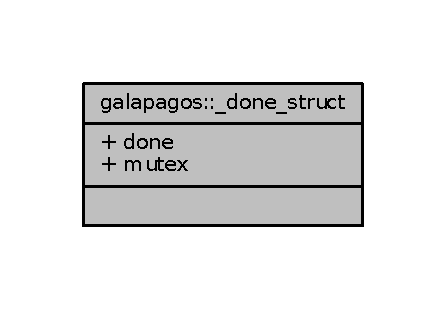
\includegraphics[width=214pt]{structgalapagos_1_1__done__struct__coll__graph}
\end{center}
\end{figure}
\subsection*{Public Attributes}
\begin{DoxyCompactItemize}
\item 
bool $\ast$ \hyperlink{structgalapagos_1_1__done__struct_a5fa9195fd41e90b6525b2beaced4de0e}{done}
\item 
std\+::mutex $\ast$ \hyperlink{structgalapagos_1_1__done__struct_ac4bd65b6a9581344f8943a499dbd5456}{mutex}
\end{DoxyCompactItemize}


\subsection{Member Data Documentation}
\index{galapagos\+::\+\_\+done\+\_\+struct@{galapagos\+::\+\_\+done\+\_\+struct}!done@{done}}
\index{done@{done}!galapagos\+::\+\_\+done\+\_\+struct@{galapagos\+::\+\_\+done\+\_\+struct}}
\subsubsection[{\texorpdfstring{done}{done}}]{\setlength{\rightskip}{0pt plus 5cm}bool$\ast$ galapagos\+::\+\_\+done\+\_\+struct\+::done}\hypertarget{structgalapagos_1_1__done__struct_a5fa9195fd41e90b6525b2beaced4de0e}{}\label{structgalapagos_1_1__done__struct_a5fa9195fd41e90b6525b2beaced4de0e}
\index{galapagos\+::\+\_\+done\+\_\+struct@{galapagos\+::\+\_\+done\+\_\+struct}!mutex@{mutex}}
\index{mutex@{mutex}!galapagos\+::\+\_\+done\+\_\+struct@{galapagos\+::\+\_\+done\+\_\+struct}}
\subsubsection[{\texorpdfstring{mutex}{mutex}}]{\setlength{\rightskip}{0pt plus 5cm}std\+::mutex$\ast$ galapagos\+::\+\_\+done\+\_\+struct\+::mutex}\hypertarget{structgalapagos_1_1__done__struct_ac4bd65b6a9581344f8943a499dbd5456}{}\label{structgalapagos_1_1__done__struct_ac4bd65b6a9581344f8943a499dbd5456}


The documentation for this struct was generated from the following file\+:\begin{DoxyCompactItemize}
\item 
\hyperlink{common_8hpp}{common.\+hpp}\end{DoxyCompactItemize}

\hypertarget{structgalapagos_1_1__num__threadsafe}{}\section{galapagos\+:\+:\+\_\+num\+\_\+threadsafe Struct Reference}
\label{structgalapagos_1_1__num__threadsafe}\index{galapagos\+::\+\_\+num\+\_\+threadsafe@{galapagos\+::\+\_\+num\+\_\+threadsafe}}


{\ttfamily \#include $<$common.\+hpp$>$}



Collaboration diagram for galapagos\+:\+:\+\_\+num\+\_\+threadsafe\+:
\nopagebreak
\begin{figure}[H]
\begin{center}
\leavevmode
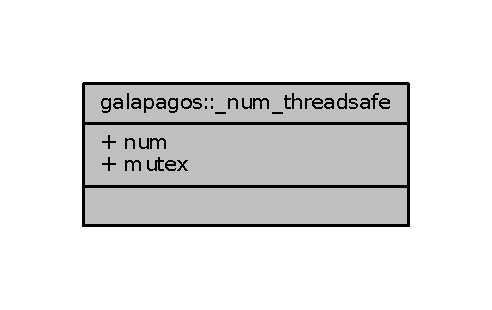
\includegraphics[width=236pt]{structgalapagos_1_1__num__threadsafe__coll__graph}
\end{center}
\end{figure}
\subsection*{Public Attributes}
\begin{DoxyCompactItemize}
\item 
int $\ast$ \hyperlink{structgalapagos_1_1__num__threadsafe_aa1de95bb520c7fa28c2edca48dc11f94}{num}
\item 
std\+::mutex $\ast$ \hyperlink{structgalapagos_1_1__num__threadsafe_ad63f0485460722ef27b2f38f9a1ab177}{mutex}
\end{DoxyCompactItemize}


\subsection{Member Data Documentation}
\index{galapagos\+::\+\_\+num\+\_\+threadsafe@{galapagos\+::\+\_\+num\+\_\+threadsafe}!mutex@{mutex}}
\index{mutex@{mutex}!galapagos\+::\+\_\+num\+\_\+threadsafe@{galapagos\+::\+\_\+num\+\_\+threadsafe}}
\subsubsection[{\texorpdfstring{mutex}{mutex}}]{\setlength{\rightskip}{0pt plus 5cm}std\+::mutex$\ast$ galapagos\+::\+\_\+num\+\_\+threadsafe\+::mutex}\hypertarget{structgalapagos_1_1__num__threadsafe_ad63f0485460722ef27b2f38f9a1ab177}{}\label{structgalapagos_1_1__num__threadsafe_ad63f0485460722ef27b2f38f9a1ab177}
\index{galapagos\+::\+\_\+num\+\_\+threadsafe@{galapagos\+::\+\_\+num\+\_\+threadsafe}!num@{num}}
\index{num@{num}!galapagos\+::\+\_\+num\+\_\+threadsafe@{galapagos\+::\+\_\+num\+\_\+threadsafe}}
\subsubsection[{\texorpdfstring{num}{num}}]{\setlength{\rightskip}{0pt plus 5cm}int$\ast$ galapagos\+::\+\_\+num\+\_\+threadsafe\+::num}\hypertarget{structgalapagos_1_1__num__threadsafe_aa1de95bb520c7fa28c2edca48dc11f94}{}\label{structgalapagos_1_1__num__threadsafe_aa1de95bb520c7fa28c2edca48dc11f94}


The documentation for this struct was generated from the following file\+:\begin{DoxyCompactItemize}
\item 
\hyperlink{common_8hpp}{common.\+hpp}\end{DoxyCompactItemize}

\hypertarget{structgalapagos_1_1buffer}{}\section{galapagos\+:\+:buffer Struct Reference}
\label{structgalapagos_1_1buffer}\index{galapagos\+::buffer@{galapagos\+::buffer}}


{\ttfamily \#include $<$galapagos\+\_\+interface.\+hpp$>$}



Collaboration diagram for galapagos\+:\+:buffer\+:
\nopagebreak
\begin{figure}[H]
\begin{center}
\leavevmode
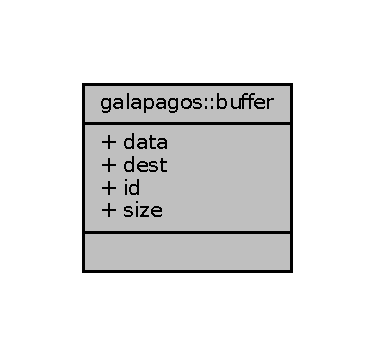
\includegraphics[width=180pt]{structgalapagos_1_1buffer__coll__graph}
\end{center}
\end{figure}
\subsection*{Public Attributes}
\begin{DoxyCompactItemize}
\item 
char \hyperlink{structgalapagos_1_1buffer_acfd1efa3acf7e85361a853e6ca117b04}{data} \mbox{[}(\hyperlink{galapagos__interface_8hpp_a1d5dab30b404fab91608086105afc78c}{M\+A\+X\+\_\+\+B\+U\+F\+F\+ER}+1)$\ast$64\mbox{]}
\item 
short \hyperlink{structgalapagos_1_1buffer_a28db83ccda617a0d33df0d0550c34245}{dest}
\item 
short \hyperlink{structgalapagos_1_1buffer_a21f882f0266b60265be7051bc608b387}{id}
\item 
size\+\_\+t \hyperlink{structgalapagos_1_1buffer_aead0014d1e1d46ec97d21896fb05f483}{size}
\end{DoxyCompactItemize}


\subsection{Detailed Description}
Struct of buffer used to store entire packets 

\subsection{Member Data Documentation}
\index{galapagos\+::buffer@{galapagos\+::buffer}!data@{data}}
\index{data@{data}!galapagos\+::buffer@{galapagos\+::buffer}}
\subsubsection[{\texorpdfstring{data}{data}}]{\setlength{\rightskip}{0pt plus 5cm}char galapagos\+::buffer\+::data\mbox{[}({\bf M\+A\+X\+\_\+\+B\+U\+F\+F\+ER}+1)$\ast$64\mbox{]}}\hypertarget{structgalapagos_1_1buffer_acfd1efa3acf7e85361a853e6ca117b04}{}\label{structgalapagos_1_1buffer_acfd1efa3acf7e85361a853e6ca117b04}
\index{galapagos\+::buffer@{galapagos\+::buffer}!dest@{dest}}
\index{dest@{dest}!galapagos\+::buffer@{galapagos\+::buffer}}
\subsubsection[{\texorpdfstring{dest}{dest}}]{\setlength{\rightskip}{0pt plus 5cm}short galapagos\+::buffer\+::dest}\hypertarget{structgalapagos_1_1buffer_a28db83ccda617a0d33df0d0550c34245}{}\label{structgalapagos_1_1buffer_a28db83ccda617a0d33df0d0550c34245}
\index{galapagos\+::buffer@{galapagos\+::buffer}!id@{id}}
\index{id@{id}!galapagos\+::buffer@{galapagos\+::buffer}}
\subsubsection[{\texorpdfstring{id}{id}}]{\setlength{\rightskip}{0pt plus 5cm}short galapagos\+::buffer\+::id}\hypertarget{structgalapagos_1_1buffer_a21f882f0266b60265be7051bc608b387}{}\label{structgalapagos_1_1buffer_a21f882f0266b60265be7051bc608b387}
\index{galapagos\+::buffer@{galapagos\+::buffer}!size@{size}}
\index{size@{size}!galapagos\+::buffer@{galapagos\+::buffer}}
\subsubsection[{\texorpdfstring{size}{size}}]{\setlength{\rightskip}{0pt plus 5cm}size\+\_\+t galapagos\+::buffer\+::size}\hypertarget{structgalapagos_1_1buffer_aead0014d1e1d46ec97d21896fb05f483}{}\label{structgalapagos_1_1buffer_aead0014d1e1d46ec97d21896fb05f483}


The documentation for this struct was generated from the following file\+:\begin{DoxyCompactItemize}
\item 
\hyperlink{galapagos__interface_8hpp}{galapagos\+\_\+interface.\+hpp}\end{DoxyCompactItemize}

\hypertarget{classgalapagos_1_1done__clean}{}\section{galapagos\+:\+:done\+\_\+clean Class Reference}
\label{classgalapagos_1_1done__clean}\index{galapagos\+::done\+\_\+clean@{galapagos\+::done\+\_\+clean}}


{\ttfamily \#include $<$common.\+hpp$>$}



Collaboration diagram for galapagos\+:\+:done\+\_\+clean\+:
\nopagebreak
\begin{figure}[H]
\begin{center}
\leavevmode
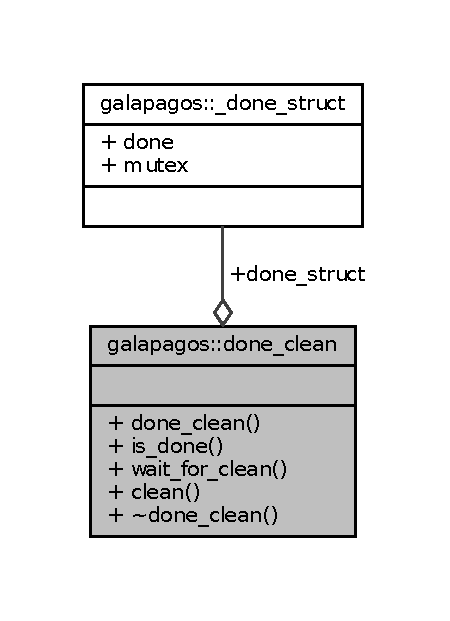
\includegraphics[width=216pt]{classgalapagos_1_1done__clean__coll__graph}
\end{center}
\end{figure}
\subsection*{Public Member Functions}
\begin{DoxyCompactItemize}
\item 
\hyperlink{classgalapagos_1_1done__clean_a5b815435d55228e92e852456b5a7b37e}{done\+\_\+clean} (bool $\ast$\+\_\+done, std\+::mutex $\ast$\+\_\+mutex)
\item 
bool \hyperlink{classgalapagos_1_1done__clean_a6e5d83850c00996e31f4b5d614ac1090}{is\+\_\+done} ()
\item 
void \hyperlink{classgalapagos_1_1done__clean_a6fbb19d798f9f3bd38a1fbaf85ab41ca}{wait\+\_\+for\+\_\+clean} ()
\item 
void \hyperlink{classgalapagos_1_1done__clean_af62181e719163c90982991b76a1c9fbb}{clean} ()
\item 
\hyperlink{classgalapagos_1_1done__clean_a4a6358456f183fa4ba794432fe2e17a0}{$\sim$done\+\_\+clean} ()
\end{DoxyCompactItemize}
\subsection*{Public Attributes}
\begin{DoxyCompactItemize}
\item 
\hyperlink{structgalapagos_1_1__done__struct}{\+\_\+done\+\_\+struct} \hyperlink{classgalapagos_1_1done__clean_ada00b712f0f38b31ed5f73981312bcd1}{done\+\_\+struct}
\end{DoxyCompactItemize}


\subsection{Constructor \& Destructor Documentation}
\index{galapagos\+::done\+\_\+clean@{galapagos\+::done\+\_\+clean}!done\+\_\+clean@{done\+\_\+clean}}
\index{done\+\_\+clean@{done\+\_\+clean}!galapagos\+::done\+\_\+clean@{galapagos\+::done\+\_\+clean}}
\subsubsection[{\texorpdfstring{done\+\_\+clean(bool $\ast$\+\_\+done, std\+::mutex $\ast$\+\_\+mutex)}{done_clean(bool *_done, std::mutex *_mutex)}}]{\setlength{\rightskip}{0pt plus 5cm}galapagos\+::done\+\_\+clean\+::done\+\_\+clean (
\begin{DoxyParamCaption}
\item[{bool $\ast$}]{\+\_\+done, }
\item[{std\+::mutex $\ast$}]{\+\_\+mutex}
\end{DoxyParamCaption}
)}\hypertarget{classgalapagos_1_1done__clean_a5b815435d55228e92e852456b5a7b37e}{}\label{classgalapagos_1_1done__clean_a5b815435d55228e92e852456b5a7b37e}
\index{galapagos\+::done\+\_\+clean@{galapagos\+::done\+\_\+clean}!````~done\+\_\+clean@{$\sim$done\+\_\+clean}}
\index{````~done\+\_\+clean@{$\sim$done\+\_\+clean}!galapagos\+::done\+\_\+clean@{galapagos\+::done\+\_\+clean}}
\subsubsection[{\texorpdfstring{$\sim$done\+\_\+clean()}{~done_clean()}}]{\setlength{\rightskip}{0pt plus 5cm}galapagos\+::done\+\_\+clean\+::$\sim$done\+\_\+clean (
\begin{DoxyParamCaption}
{}
\end{DoxyParamCaption}
)\hspace{0.3cm}{\ttfamily [inline]}}\hypertarget{classgalapagos_1_1done__clean_a4a6358456f183fa4ba794432fe2e17a0}{}\label{classgalapagos_1_1done__clean_a4a6358456f183fa4ba794432fe2e17a0}


\subsection{Member Function Documentation}
\index{galapagos\+::done\+\_\+clean@{galapagos\+::done\+\_\+clean}!clean@{clean}}
\index{clean@{clean}!galapagos\+::done\+\_\+clean@{galapagos\+::done\+\_\+clean}}
\subsubsection[{\texorpdfstring{clean()}{clean()}}]{\setlength{\rightskip}{0pt plus 5cm}void galapagos\+::done\+\_\+clean\+::clean (
\begin{DoxyParamCaption}
{}
\end{DoxyParamCaption}
)}\hypertarget{classgalapagos_1_1done__clean_af62181e719163c90982991b76a1c9fbb}{}\label{classgalapagos_1_1done__clean_af62181e719163c90982991b76a1c9fbb}
\index{galapagos\+::done\+\_\+clean@{galapagos\+::done\+\_\+clean}!is\+\_\+done@{is\+\_\+done}}
\index{is\+\_\+done@{is\+\_\+done}!galapagos\+::done\+\_\+clean@{galapagos\+::done\+\_\+clean}}
\subsubsection[{\texorpdfstring{is\+\_\+done()}{is_done()}}]{\setlength{\rightskip}{0pt plus 5cm}bool galapagos\+::done\+\_\+clean\+::is\+\_\+done (
\begin{DoxyParamCaption}
{}
\end{DoxyParamCaption}
)}\hypertarget{classgalapagos_1_1done__clean_a6e5d83850c00996e31f4b5d614ac1090}{}\label{classgalapagos_1_1done__clean_a6e5d83850c00996e31f4b5d614ac1090}
\index{galapagos\+::done\+\_\+clean@{galapagos\+::done\+\_\+clean}!wait\+\_\+for\+\_\+clean@{wait\+\_\+for\+\_\+clean}}
\index{wait\+\_\+for\+\_\+clean@{wait\+\_\+for\+\_\+clean}!galapagos\+::done\+\_\+clean@{galapagos\+::done\+\_\+clean}}
\subsubsection[{\texorpdfstring{wait\+\_\+for\+\_\+clean()}{wait_for_clean()}}]{\setlength{\rightskip}{0pt plus 5cm}void galapagos\+::done\+\_\+clean\+::wait\+\_\+for\+\_\+clean (
\begin{DoxyParamCaption}
{}
\end{DoxyParamCaption}
)}\hypertarget{classgalapagos_1_1done__clean_a6fbb19d798f9f3bd38a1fbaf85ab41ca}{}\label{classgalapagos_1_1done__clean_a6fbb19d798f9f3bd38a1fbaf85ab41ca}


\subsection{Member Data Documentation}
\index{galapagos\+::done\+\_\+clean@{galapagos\+::done\+\_\+clean}!done\+\_\+struct@{done\+\_\+struct}}
\index{done\+\_\+struct@{done\+\_\+struct}!galapagos\+::done\+\_\+clean@{galapagos\+::done\+\_\+clean}}
\subsubsection[{\texorpdfstring{done\+\_\+struct}{done_struct}}]{\setlength{\rightskip}{0pt plus 5cm}{\bf \+\_\+done\+\_\+struct} galapagos\+::done\+\_\+clean\+::done\+\_\+struct}\hypertarget{classgalapagos_1_1done__clean_ada00b712f0f38b31ed5f73981312bcd1}{}\label{classgalapagos_1_1done__clean_ada00b712f0f38b31ed5f73981312bcd1}


The documentation for this class was generated from the following files\+:\begin{DoxyCompactItemize}
\item 
\hyperlink{common_8hpp}{common.\+hpp}\item 
\hyperlink{common_8cpp}{common.\+cpp}\end{DoxyCompactItemize}

\hypertarget{classgalapagos_1_1external__driver}{}\section{galapagos\+:\+:external\+\_\+driver$<$ T $>$ Class Template Reference}
\label{classgalapagos_1_1external__driver}\index{galapagos\+::external\+\_\+driver$<$ T $>$@{galapagos\+::external\+\_\+driver$<$ T $>$}}


{\ttfamily \#include $<$galapagos\+\_\+external\+\_\+driver.\+hpp$>$}



Inheritance diagram for galapagos\+:\+:external\+\_\+driver$<$ T $>$\+:
\nopagebreak
\begin{figure}[H]
\begin{center}
\leavevmode
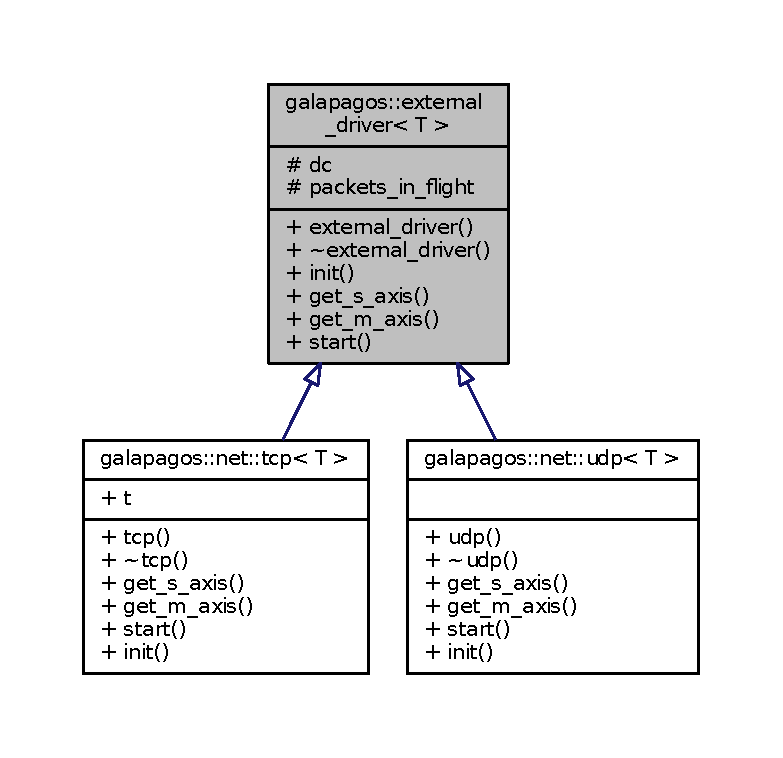
\includegraphics[width=350pt]{classgalapagos_1_1external__driver__inherit__graph}
\end{center}
\end{figure}


Collaboration diagram for galapagos\+:\+:external\+\_\+driver$<$ T $>$\+:
\nopagebreak
\begin{figure}[H]
\begin{center}
\leavevmode
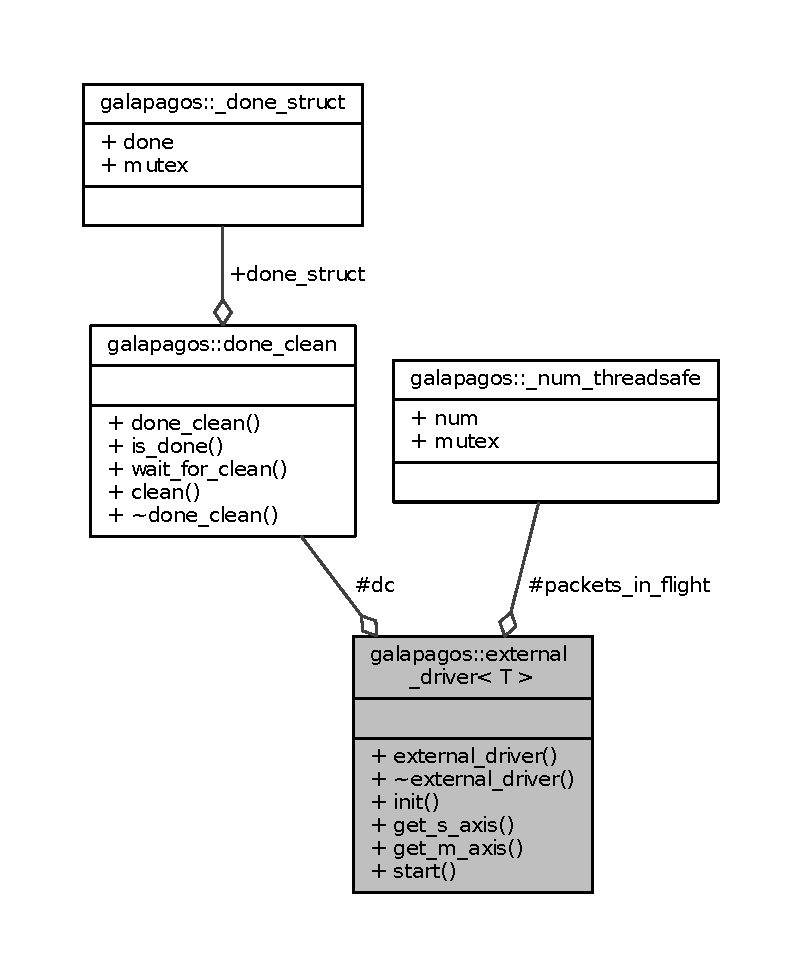
\includegraphics[width=350pt]{classgalapagos_1_1external__driver__coll__graph}
\end{center}
\end{figure}
\subsection*{Public Member Functions}
\begin{DoxyCompactItemize}
\item 
\hyperlink{classgalapagos_1_1external__driver_ae3ee965ba34df3e8c29f5c722d1ad51e}{external\+\_\+driver} ()
\item 
\hyperlink{classgalapagos_1_1external__driver_ab89f9aca8f2f88e3aef2eef0335022d7}{$\sim$external\+\_\+driver} ()
\item 
virtual void \hyperlink{classgalapagos_1_1external__driver_ab8b753325b02ee15efe16158cd3fe119}{init} (\hyperlink{classgalapagos_1_1done__clean}{done\+\_\+clean} $\ast$\+\_\+dc, int $\ast$\+\_\+packets\+\_\+in\+\_\+flight, std\+::mutex $\ast$\+\_\+mutex\+\_\+packets\+\_\+in\+\_\+flight)=0
\item 
virtual \hyperlink{classgalapagos_1_1interface}{interface}$<$ \hyperlink{test_8cpp_a0658ceffa730c765d449bb3d21871b5f}{T} $>$ $\ast$ \hyperlink{classgalapagos_1_1external__driver_aded446e9ebbdd03b461f336045aa7cd2}{get\+\_\+s\+\_\+axis} ()=0
\item 
virtual \hyperlink{classgalapagos_1_1interface}{interface}$<$ \hyperlink{test_8cpp_a0658ceffa730c765d449bb3d21871b5f}{T} $>$ $\ast$ \hyperlink{classgalapagos_1_1external__driver_abc7938fd7247c7404441473da71a357e}{get\+\_\+m\+\_\+axis} ()=0
\item 
virtual void \hyperlink{classgalapagos_1_1external__driver_a7eacf72788a4ce6976499e36f1b7b3a6}{start} ()=0
\end{DoxyCompactItemize}
\subsection*{Protected Attributes}
\begin{DoxyCompactItemize}
\item 
\hyperlink{classgalapagos_1_1done__clean}{done\+\_\+clean} $\ast$ \hyperlink{classgalapagos_1_1external__driver_aa868bceef97438040dbb3d795e96cd9e}{dc}
\item 
\hyperlink{structgalapagos_1_1__num__threadsafe}{\+\_\+num\+\_\+threadsafe} \hyperlink{classgalapagos_1_1external__driver_a66c3c0c6b022c1335beda3de4f18ced8}{packets\+\_\+in\+\_\+flight}
\end{DoxyCompactItemize}


\subsection{Constructor \& Destructor Documentation}
\index{galapagos\+::external\+\_\+driver@{galapagos\+::external\+\_\+driver}!external\+\_\+driver@{external\+\_\+driver}}
\index{external\+\_\+driver@{external\+\_\+driver}!galapagos\+::external\+\_\+driver@{galapagos\+::external\+\_\+driver}}
\subsubsection[{\texorpdfstring{external\+\_\+driver()}{external_driver()}}]{\setlength{\rightskip}{0pt plus 5cm}template$<$class T $>$ {\bf galapagos\+::external\+\_\+driver}$<$ {\bf T} $>$\+::{\bf external\+\_\+driver} (
\begin{DoxyParamCaption}
{}
\end{DoxyParamCaption}
)\hspace{0.3cm}{\ttfamily [inline]}}\hypertarget{classgalapagos_1_1external__driver_ae3ee965ba34df3e8c29f5c722d1ad51e}{}\label{classgalapagos_1_1external__driver_ae3ee965ba34df3e8c29f5c722d1ad51e}
\index{galapagos\+::external\+\_\+driver@{galapagos\+::external\+\_\+driver}!````~external\+\_\+driver@{$\sim$external\+\_\+driver}}
\index{````~external\+\_\+driver@{$\sim$external\+\_\+driver}!galapagos\+::external\+\_\+driver@{galapagos\+::external\+\_\+driver}}
\subsubsection[{\texorpdfstring{$\sim$external\+\_\+driver()}{~external_driver()}}]{\setlength{\rightskip}{0pt plus 5cm}template$<$class T $>$ {\bf galapagos\+::external\+\_\+driver}$<$ {\bf T} $>$\+::$\sim${\bf external\+\_\+driver} (
\begin{DoxyParamCaption}
{}
\end{DoxyParamCaption}
)\hspace{0.3cm}{\ttfamily [inline]}}\hypertarget{classgalapagos_1_1external__driver_ab89f9aca8f2f88e3aef2eef0335022d7}{}\label{classgalapagos_1_1external__driver_ab89f9aca8f2f88e3aef2eef0335022d7}


\subsection{Member Function Documentation}
\index{galapagos\+::external\+\_\+driver@{galapagos\+::external\+\_\+driver}!get\+\_\+m\+\_\+axis@{get\+\_\+m\+\_\+axis}}
\index{get\+\_\+m\+\_\+axis@{get\+\_\+m\+\_\+axis}!galapagos\+::external\+\_\+driver@{galapagos\+::external\+\_\+driver}}
\subsubsection[{\texorpdfstring{get\+\_\+m\+\_\+axis()=0}{get_m_axis()=0}}]{\setlength{\rightskip}{0pt plus 5cm}template$<$class T $>$ virtual {\bf interface}$<${\bf T}$>$$\ast$ {\bf galapagos\+::external\+\_\+driver}$<$ {\bf T} $>$\+::get\+\_\+m\+\_\+axis (
\begin{DoxyParamCaption}
{}
\end{DoxyParamCaption}
)\hspace{0.3cm}{\ttfamily [pure virtual]}}\hypertarget{classgalapagos_1_1external__driver_abc7938fd7247c7404441473da71a357e}{}\label{classgalapagos_1_1external__driver_abc7938fd7247c7404441473da71a357e}


Implemented in \hyperlink{classgalapagos_1_1net_1_1tcp_a47f42325519b0dda4c0157f1d897ed75}{galapagos\+::net\+::tcp$<$ T $>$}, and \hyperlink{classgalapagos_1_1net_1_1udp_a5ab392ec0015391f4428b34463d62d06}{galapagos\+::net\+::udp$<$ T $>$}.

\index{galapagos\+::external\+\_\+driver@{galapagos\+::external\+\_\+driver}!get\+\_\+s\+\_\+axis@{get\+\_\+s\+\_\+axis}}
\index{get\+\_\+s\+\_\+axis@{get\+\_\+s\+\_\+axis}!galapagos\+::external\+\_\+driver@{galapagos\+::external\+\_\+driver}}
\subsubsection[{\texorpdfstring{get\+\_\+s\+\_\+axis()=0}{get_s_axis()=0}}]{\setlength{\rightskip}{0pt plus 5cm}template$<$class T $>$ virtual {\bf interface}$<${\bf T}$>$$\ast$ {\bf galapagos\+::external\+\_\+driver}$<$ {\bf T} $>$\+::get\+\_\+s\+\_\+axis (
\begin{DoxyParamCaption}
{}
\end{DoxyParamCaption}
)\hspace{0.3cm}{\ttfamily [pure virtual]}}\hypertarget{classgalapagos_1_1external__driver_aded446e9ebbdd03b461f336045aa7cd2}{}\label{classgalapagos_1_1external__driver_aded446e9ebbdd03b461f336045aa7cd2}


Implemented in \hyperlink{classgalapagos_1_1net_1_1tcp_ac9f3db01e1d6e9bf0bc7527fabf3543a}{galapagos\+::net\+::tcp$<$ T $>$}, and \hyperlink{classgalapagos_1_1net_1_1udp_aed1c1ca798141a5eb83382b384ede0c1}{galapagos\+::net\+::udp$<$ T $>$}.

\index{galapagos\+::external\+\_\+driver@{galapagos\+::external\+\_\+driver}!init@{init}}
\index{init@{init}!galapagos\+::external\+\_\+driver@{galapagos\+::external\+\_\+driver}}
\subsubsection[{\texorpdfstring{init(done\+\_\+clean $\ast$\+\_\+dc, int $\ast$\+\_\+packets\+\_\+in\+\_\+flight, std\+::mutex $\ast$\+\_\+mutex\+\_\+packets\+\_\+in\+\_\+flight)=0}{init(done_clean *_dc, int *_packets_in_flight, std::mutex *_mutex_packets_in_flight)=0}}]{\setlength{\rightskip}{0pt plus 5cm}template$<$class T $>$ virtual void {\bf galapagos\+::external\+\_\+driver}$<$ {\bf T} $>$\+::init (
\begin{DoxyParamCaption}
\item[{{\bf done\+\_\+clean} $\ast$}]{\+\_\+dc, }
\item[{int $\ast$}]{\+\_\+packets\+\_\+in\+\_\+flight, }
\item[{std\+::mutex $\ast$}]{\+\_\+mutex\+\_\+packets\+\_\+in\+\_\+flight}
\end{DoxyParamCaption}
)\hspace{0.3cm}{\ttfamily [pure virtual]}}\hypertarget{classgalapagos_1_1external__driver_ab8b753325b02ee15efe16158cd3fe119}{}\label{classgalapagos_1_1external__driver_ab8b753325b02ee15efe16158cd3fe119}


Implemented in \hyperlink{classgalapagos_1_1net_1_1tcp_a10e2ca93acd1562162b2a49400be1292}{galapagos\+::net\+::tcp$<$ T $>$}, and \hyperlink{classgalapagos_1_1net_1_1udp_a0a071fe7943e7ff4d59640dd39392b50}{galapagos\+::net\+::udp$<$ T $>$}.

\index{galapagos\+::external\+\_\+driver@{galapagos\+::external\+\_\+driver}!start@{start}}
\index{start@{start}!galapagos\+::external\+\_\+driver@{galapagos\+::external\+\_\+driver}}
\subsubsection[{\texorpdfstring{start()=0}{start()=0}}]{\setlength{\rightskip}{0pt plus 5cm}template$<$class T $>$ virtual void {\bf galapagos\+::external\+\_\+driver}$<$ {\bf T} $>$\+::start (
\begin{DoxyParamCaption}
{}
\end{DoxyParamCaption}
)\hspace{0.3cm}{\ttfamily [pure virtual]}}\hypertarget{classgalapagos_1_1external__driver_a7eacf72788a4ce6976499e36f1b7b3a6}{}\label{classgalapagos_1_1external__driver_a7eacf72788a4ce6976499e36f1b7b3a6}


Implemented in \hyperlink{classgalapagos_1_1net_1_1tcp_ad792d3c67e6e8a79cb18a6d0c4aaecda}{galapagos\+::net\+::tcp$<$ T $>$}, and \hyperlink{classgalapagos_1_1net_1_1udp_acb79ddb76eeb80fbf775cba76f251ac8}{galapagos\+::net\+::udp$<$ T $>$}.



\subsection{Member Data Documentation}
\index{galapagos\+::external\+\_\+driver@{galapagos\+::external\+\_\+driver}!dc@{dc}}
\index{dc@{dc}!galapagos\+::external\+\_\+driver@{galapagos\+::external\+\_\+driver}}
\subsubsection[{\texorpdfstring{dc}{dc}}]{\setlength{\rightskip}{0pt plus 5cm}template$<$class T $>$ {\bf done\+\_\+clean}$\ast$ {\bf galapagos\+::external\+\_\+driver}$<$ {\bf T} $>$\+::dc\hspace{0.3cm}{\ttfamily [protected]}}\hypertarget{classgalapagos_1_1external__driver_aa868bceef97438040dbb3d795e96cd9e}{}\label{classgalapagos_1_1external__driver_aa868bceef97438040dbb3d795e96cd9e}
\index{galapagos\+::external\+\_\+driver@{galapagos\+::external\+\_\+driver}!packets\+\_\+in\+\_\+flight@{packets\+\_\+in\+\_\+flight}}
\index{packets\+\_\+in\+\_\+flight@{packets\+\_\+in\+\_\+flight}!galapagos\+::external\+\_\+driver@{galapagos\+::external\+\_\+driver}}
\subsubsection[{\texorpdfstring{packets\+\_\+in\+\_\+flight}{packets_in_flight}}]{\setlength{\rightskip}{0pt plus 5cm}template$<$class T $>$ {\bf \+\_\+num\+\_\+threadsafe} {\bf galapagos\+::external\+\_\+driver}$<$ {\bf T} $>$\+::packets\+\_\+in\+\_\+flight\hspace{0.3cm}{\ttfamily [protected]}}\hypertarget{classgalapagos_1_1external__driver_a66c3c0c6b022c1335beda3de4f18ced8}{}\label{classgalapagos_1_1external__driver_a66c3c0c6b022c1335beda3de4f18ced8}


The documentation for this class was generated from the following file\+:\begin{DoxyCompactItemize}
\item 
\hyperlink{galapagos__external__driver_8hpp}{galapagos\+\_\+external\+\_\+driver.\+hpp}\end{DoxyCompactItemize}

\hypertarget{classgalapagos_1_1interface}{}\section{galapagos\+:\+:interface$<$ T $>$ Class Template Reference}
\label{classgalapagos_1_1interface}\index{galapagos\+::interface$<$ T $>$@{galapagos\+::interface$<$ T $>$}}


Class for the Galapagos Interface.  




{\ttfamily \#include $<$galapagos\+\_\+interface.\+hpp$>$}



Collaboration diagram for galapagos\+:\+:interface$<$ T $>$\+:
\nopagebreak
\begin{figure}[H]
\begin{center}
\leavevmode
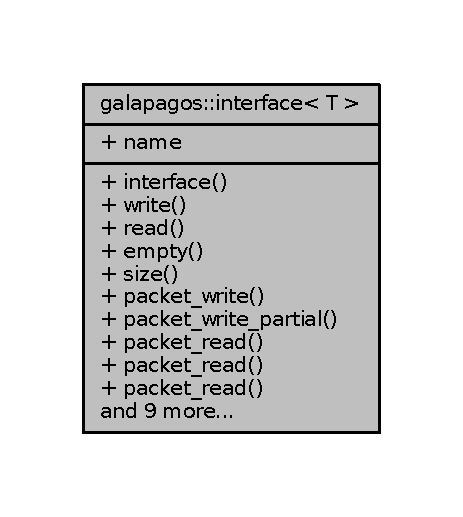
\includegraphics[width=222pt]{classgalapagos_1_1interface__coll__graph}
\end{center}
\end{figure}
\subsection*{Public Member Functions}
\begin{DoxyCompactItemize}
\item 
\hyperlink{classgalapagos_1_1interface_a63cb49d57ceba5e8c98bba9525799a39}{interface} (std\+::string \+\_\+name)
\item 
void \hyperlink{classgalapagos_1_1interface_a4b3dd138cac79282418844e588e2535b}{write} (\hyperlink{structgalapagos_1_1stream__packet}{galapagos\+::stream\+\_\+packet}$<$ \hyperlink{test_8cpp_a0658ceffa730c765d449bb3d21871b5f}{T} $>$ gps)
\item 
\hyperlink{structgalapagos_1_1stream__packet}{galapagos\+::stream\+\_\+packet}$<$ \hyperlink{test_8cpp_a0658ceffa730c765d449bb3d21871b5f}{T} $>$ \hyperlink{classgalapagos_1_1interface_a5b6366fdfa799f10d782d9f26dccd537}{read} ()
\item 
bool \hyperlink{classgalapagos_1_1interface_af856cabc1eae494cec44f0db63723f90}{empty} ()
\item 
size\+\_\+t \hyperlink{classgalapagos_1_1interface_a385b790d8de8fa2bab099d23dbfe783e}{size} ()
\item 
void \hyperlink{classgalapagos_1_1interface_a1369e3db6102f97c9d34e48de905ecd4}{packet\+\_\+write} (char $\ast$data, int \hyperlink{classgalapagos_1_1interface_a385b790d8de8fa2bab099d23dbfe783e}{size}, short dest, short id)
\item 
void \hyperlink{classgalapagos_1_1interface_a815dfac71a7f639f62dbe0a0d9347624}{packet\+\_\+write\+\_\+partial} (char $\ast$data, int \hyperlink{classgalapagos_1_1interface_a385b790d8de8fa2bab099d23dbfe783e}{size}, bool assert\+\_\+last)
\item 
char $\ast$ \hyperlink{classgalapagos_1_1interface_ad5cc5346287afb304531bcd35667ee4e}{packet\+\_\+read} (size\+\_\+t $\ast$\hyperlink{classgalapagos_1_1interface_a385b790d8de8fa2bab099d23dbfe783e}{size}, short $\ast$dest, short $\ast$id)
\item 
void \hyperlink{classgalapagos_1_1interface_a3e42b3aa2133d0f05c680bfc8fae0195}{packet\+\_\+read} (char $\ast$mem, size\+\_\+t $\ast$\hyperlink{classgalapagos_1_1interface_a385b790d8de8fa2bab099d23dbfe783e}{size}, short $\ast$dest, short $\ast$id)
\item 
char $\ast$ \hyperlink{classgalapagos_1_1interface_a9c87f2c9fe9ed9ee0449dc014e160d16}{packet\+\_\+read} (size\+\_\+t $\ast$\+\_\+size)
\item 
void \hyperlink{classgalapagos_1_1interface_a087c18c30205c94e6bc458e5bf99f7e6}{set\+\_\+filter} (size\+\_\+t pos, char byte)
\item 
short \hyperlink{classgalapagos_1_1interface_ac39b859a468e02a0e6b6ca50f042f79d}{get\+\_\+head\+\_\+dest} ()
\item 
std\+::mutex $\ast$ \hyperlink{classgalapagos_1_1interface_a334efdcb21695a5eef218c3a85fbfecd}{get\+\_\+mutex} ()
\item 
std\+::list$<$ \hyperlink{structgalapagos_1_1buffer}{galapagos\+::buffer} $>$ $\ast$ \hyperlink{classgalapagos_1_1interface_a9becb63ba4b22e0b9454f779acb98831}{get\+\_\+packets} ()
\item 
std\+::condition\+\_\+variable $\ast$ \hyperlink{classgalapagos_1_1interface_a4be570f46f0b8e1033e1ad9fcb6dbebb}{get\+\_\+cv} ()
\item 
void \hyperlink{classgalapagos_1_1interface_a5997a6189db1f967df01d0a9fb9e1990}{splice} (\hyperlink{classgalapagos_1_1interface}{galapagos\+::interface}$<$ \hyperlink{test_8cpp_a0658ceffa730c765d449bb3d21871b5f}{T} $>$ $\ast$\+\_\+interface)
\item 
std\+::list$<$ \hyperlink{structgalapagos_1_1buffer}{buffer} $>$\+::iterator \hyperlink{classgalapagos_1_1interface_ab828fd748b635db64e13198d328fae79}{get\+\_\+unsafe\+\_\+head\+\_\+buffer} ()
\item 
void \hyperlink{classgalapagos_1_1interface_a5002553bd7196789fac8adcd8d837f42}{delete\+\_\+unsafe\+\_\+head\+\_\+buffer} ()
\item 
std\+::list$<$ \hyperlink{structgalapagos_1_1buffer}{buffer} $>$ $\ast$ \hyperlink{classgalapagos_1_1interface_ae6f7ed4a44a09ea0871e83a2d508fa13}{get\+\_\+unsafe\+\_\+list} ()
\end{DoxyCompactItemize}
\subsection*{Public Attributes}
\begin{DoxyCompactItemize}
\item 
std\+::string \hyperlink{classgalapagos_1_1interface_a5c9e7d1a9830311b74acd055ccd5f3f6}{name}
\end{DoxyCompactItemize}


\subsection{Detailed Description}
\subsubsection*{template$<$class T$>$\\*
class galapagos\+::interface$<$ T $>$}

Class for the Galapagos Interface. 

Threadsafe for single producer, single consumer. Gives user an interface to read/write flits and entire packets. Packets internally are stored in linked-\/list and can be spliced to other linked-\/lists. The flit interface reads from the head packet of the linked-\/list and writes to the tail packet. \begin{DoxyAuthor}{Author}
Naif Tarafdar 
\end{DoxyAuthor}
\begin{DoxyDate}{Date}
April 20, 2019 
\end{DoxyDate}


\subsection{Constructor \& Destructor Documentation}
\index{galapagos\+::interface@{galapagos\+::interface}!interface@{interface}}
\index{interface@{interface}!galapagos\+::interface@{galapagos\+::interface}}
\subsubsection[{\texorpdfstring{interface(std\+::string \+\_\+name)}{interface(std::string _name)}}]{\setlength{\rightskip}{0pt plus 5cm}template$<$class T $>$ {\bf galapagos\+::interface}$<$ {\bf T} $>$\+::{\bf interface} (
\begin{DoxyParamCaption}
\item[{std\+::string}]{\+\_\+name}
\end{DoxyParamCaption}
)}\hypertarget{classgalapagos_1_1interface_a63cb49d57ceba5e8c98bba9525799a39}{}\label{classgalapagos_1_1interface_a63cb49d57ceba5e8c98bba9525799a39}


\subsection{Member Function Documentation}
\index{galapagos\+::interface@{galapagos\+::interface}!delete\+\_\+unsafe\+\_\+head\+\_\+buffer@{delete\+\_\+unsafe\+\_\+head\+\_\+buffer}}
\index{delete\+\_\+unsafe\+\_\+head\+\_\+buffer@{delete\+\_\+unsafe\+\_\+head\+\_\+buffer}!galapagos\+::interface@{galapagos\+::interface}}
\subsubsection[{\texorpdfstring{delete\+\_\+unsafe\+\_\+head\+\_\+buffer()}{delete_unsafe_head_buffer()}}]{\setlength{\rightskip}{0pt plus 5cm}template$<$class T $>$ void {\bf galapagos\+::interface}$<$ {\bf T} $>$\+::delete\+\_\+unsafe\+\_\+head\+\_\+buffer (
\begin{DoxyParamCaption}
{}
\end{DoxyParamCaption}
)}\hypertarget{classgalapagos_1_1interface_a5002553bd7196789fac8adcd8d837f42}{}\label{classgalapagos_1_1interface_a5002553bd7196789fac8adcd8d837f42}
\index{galapagos\+::interface@{galapagos\+::interface}!empty@{empty}}
\index{empty@{empty}!galapagos\+::interface@{galapagos\+::interface}}
\subsubsection[{\texorpdfstring{empty()}{empty()}}]{\setlength{\rightskip}{0pt plus 5cm}template$<$class T $>$ bool {\bf galapagos\+::interface}$<$ {\bf T} $>$\+::empty (
\begin{DoxyParamCaption}
{}
\end{DoxyParamCaption}
)}\hypertarget{classgalapagos_1_1interface_af856cabc1eae494cec44f0db63723f90}{}\label{classgalapagos_1_1interface_af856cabc1eae494cec44f0db63723f90}
Get if buffer is empty 
\begin{DoxyTemplParams}{Template Parameters}
{\em T} & the type of data used within each galapagos packet (default ap\+\_\+uint$<$64$>$) \\
\hline
\end{DoxyTemplParams}
\begin{DoxyReturn}{Returns}
bool representing if buffer is empty 
\end{DoxyReturn}
\index{galapagos\+::interface@{galapagos\+::interface}!get\+\_\+cv@{get\+\_\+cv}}
\index{get\+\_\+cv@{get\+\_\+cv}!galapagos\+::interface@{galapagos\+::interface}}
\subsubsection[{\texorpdfstring{get\+\_\+cv()}{get_cv()}}]{\setlength{\rightskip}{0pt plus 5cm}template$<$class T $>$ std\+::condition\+\_\+variable $\ast$ {\bf galapagos\+::interface}$<$ {\bf T} $>$\+::get\+\_\+cv (
\begin{DoxyParamCaption}
{}
\end{DoxyParamCaption}
)}\hypertarget{classgalapagos_1_1interface_a4be570f46f0b8e1033e1ad9fcb6dbebb}{}\label{classgalapagos_1_1interface_a4be570f46f0b8e1033e1ad9fcb6dbebb}
Get pointer to list of cv, needed to splice \begin{DoxyReturn}{Returns}
pointer to list of packets 
\end{DoxyReturn}
\index{galapagos\+::interface@{galapagos\+::interface}!get\+\_\+head\+\_\+dest@{get\+\_\+head\+\_\+dest}}
\index{get\+\_\+head\+\_\+dest@{get\+\_\+head\+\_\+dest}!galapagos\+::interface@{galapagos\+::interface}}
\subsubsection[{\texorpdfstring{get\+\_\+head\+\_\+dest()}{get_head_dest()}}]{\setlength{\rightskip}{0pt plus 5cm}template$<$class T $>$ short {\bf galapagos\+::interface}$<$ {\bf T} $>$\+::get\+\_\+head\+\_\+dest (
\begin{DoxyParamCaption}
{}
\end{DoxyParamCaption}
)}\hypertarget{classgalapagos_1_1interface_ac39b859a468e02a0e6b6ca50f042f79d}{}\label{classgalapagos_1_1interface_ac39b859a468e02a0e6b6ca50f042f79d}
\index{galapagos\+::interface@{galapagos\+::interface}!get\+\_\+mutex@{get\+\_\+mutex}}
\index{get\+\_\+mutex@{get\+\_\+mutex}!galapagos\+::interface@{galapagos\+::interface}}
\subsubsection[{\texorpdfstring{get\+\_\+mutex()}{get_mutex()}}]{\setlength{\rightskip}{0pt plus 5cm}template$<$class T $>$ std\+::mutex $\ast$ {\bf galapagos\+::interface}$<$ {\bf T} $>$\+::get\+\_\+mutex (
\begin{DoxyParamCaption}
{}
\end{DoxyParamCaption}
)}\hypertarget{classgalapagos_1_1interface_a334efdcb21695a5eef218c3a85fbfecd}{}\label{classgalapagos_1_1interface_a334efdcb21695a5eef218c3a85fbfecd}
Get pointer to mutex, needed to splice \begin{DoxyReturn}{Returns}
pointer to mutex for list 
\end{DoxyReturn}
\index{galapagos\+::interface@{galapagos\+::interface}!get\+\_\+packets@{get\+\_\+packets}}
\index{get\+\_\+packets@{get\+\_\+packets}!galapagos\+::interface@{galapagos\+::interface}}
\subsubsection[{\texorpdfstring{get\+\_\+packets()}{get_packets()}}]{\setlength{\rightskip}{0pt plus 5cm}template$<$class T $>$ std\+::list$<$ {\bf galapagos\+::buffer} $>$ $\ast$ {\bf galapagos\+::interface}$<$ {\bf T} $>$\+::get\+\_\+packets (
\begin{DoxyParamCaption}
{}
\end{DoxyParamCaption}
)}\hypertarget{classgalapagos_1_1interface_a9becb63ba4b22e0b9454f779acb98831}{}\label{classgalapagos_1_1interface_a9becb63ba4b22e0b9454f779acb98831}
Get pointer to list of packets, needed to splice \begin{DoxyReturn}{Returns}
pointer to list of packets 
\end{DoxyReturn}
\index{galapagos\+::interface@{galapagos\+::interface}!get\+\_\+unsafe\+\_\+head\+\_\+buffer@{get\+\_\+unsafe\+\_\+head\+\_\+buffer}}
\index{get\+\_\+unsafe\+\_\+head\+\_\+buffer@{get\+\_\+unsafe\+\_\+head\+\_\+buffer}!galapagos\+::interface@{galapagos\+::interface}}
\subsubsection[{\texorpdfstring{get\+\_\+unsafe\+\_\+head\+\_\+buffer()}{get_unsafe_head_buffer()}}]{\setlength{\rightskip}{0pt plus 5cm}template$<$class T $>$ std\+::list$<$ {\bf galapagos\+::buffer} $>$\+::iterator {\bf galapagos\+::interface}$<$ {\bf T} $>$\+::get\+\_\+unsafe\+\_\+head\+\_\+buffer (
\begin{DoxyParamCaption}
{}
\end{DoxyParamCaption}
)}\hypertarget{classgalapagos_1_1interface_ab828fd748b635db64e13198d328fae79}{}\label{classgalapagos_1_1interface_ab828fd748b635db64e13198d328fae79}
\index{galapagos\+::interface@{galapagos\+::interface}!get\+\_\+unsafe\+\_\+list@{get\+\_\+unsafe\+\_\+list}}
\index{get\+\_\+unsafe\+\_\+list@{get\+\_\+unsafe\+\_\+list}!galapagos\+::interface@{galapagos\+::interface}}
\subsubsection[{\texorpdfstring{get\+\_\+unsafe\+\_\+list()}{get_unsafe_list()}}]{\setlength{\rightskip}{0pt plus 5cm}template$<$class T $>$ std\+::list$<$ {\bf galapagos\+::buffer} $>$ $\ast$ {\bf galapagos\+::interface}$<$ {\bf T} $>$\+::get\+\_\+unsafe\+\_\+list (
\begin{DoxyParamCaption}
{}
\end{DoxyParamCaption}
)}\hypertarget{classgalapagos_1_1interface_ae6f7ed4a44a09ea0871e83a2d508fa13}{}\label{classgalapagos_1_1interface_ae6f7ed4a44a09ea0871e83a2d508fa13}
\index{galapagos\+::interface@{galapagos\+::interface}!packet\+\_\+read@{packet\+\_\+read}}
\index{packet\+\_\+read@{packet\+\_\+read}!galapagos\+::interface@{galapagos\+::interface}}
\subsubsection[{\texorpdfstring{packet\+\_\+read(size\+\_\+t $\ast$size, short $\ast$dest, short $\ast$id)}{packet_read(size_t *size, short *dest, short *id)}}]{\setlength{\rightskip}{0pt plus 5cm}template$<$class T $>$ char $\ast$ {\bf galapagos\+::interface}$<$ {\bf T} $>$\+::packet\+\_\+read (
\begin{DoxyParamCaption}
\item[{size\+\_\+t $\ast$}]{\+\_\+size, }
\item[{short $\ast$}]{\+\_\+dest, }
\item[{short $\ast$}]{\+\_\+id}
\end{DoxyParamCaption}
)}\hypertarget{classgalapagos_1_1interface_ad5cc5346287afb304531bcd35667ee4e}{}\label{classgalapagos_1_1interface_ad5cc5346287afb304531bcd35667ee4e}
Executes a packet read, this function is not portable between C\+PU and F\+P\+GA. Please be careful to rewrite C\+PU functions to use an individual flit write when porting to H\+LS 
\begin{DoxyTemplParams}{Template Parameters}
{\em T} & the type of data used within each galapagos packet (default ap\+\_\+uint$<$64$>$) \\
\hline
\end{DoxyTemplParams}

\begin{DoxyParams}[1]{Parameters}
\mbox{\tt out}  & {\em \+\_\+size} & size of buffer \\
\hline
\mbox{\tt out}  & {\em \+\_\+dest} & dest of buffer \\
\hline
\mbox{\tt out}  & {\em \+\_\+id} & id of buffer \\
\hline
\end{DoxyParams}
\begin{DoxyReturn}{Returns}
buffer pointing to batch of data 
\end{DoxyReturn}
\index{galapagos\+::interface@{galapagos\+::interface}!packet\+\_\+read@{packet\+\_\+read}}
\index{packet\+\_\+read@{packet\+\_\+read}!galapagos\+::interface@{galapagos\+::interface}}
\subsubsection[{\texorpdfstring{packet\+\_\+read(char $\ast$mem, size\+\_\+t $\ast$size, short $\ast$dest, short $\ast$id)}{packet_read(char *mem, size_t *size, short *dest, short *id)}}]{\setlength{\rightskip}{0pt plus 5cm}template$<$class T $>$ void {\bf galapagos\+::interface}$<$ {\bf T} $>$\+::packet\+\_\+read (
\begin{DoxyParamCaption}
\item[{char $\ast$}]{mem, }
\item[{size\+\_\+t $\ast$}]{\+\_\+size, }
\item[{short $\ast$}]{\+\_\+dest, }
\item[{short $\ast$}]{\+\_\+id}
\end{DoxyParamCaption}
)}\hypertarget{classgalapagos_1_1interface_a3e42b3aa2133d0f05c680bfc8fae0195}{}\label{classgalapagos_1_1interface_a3e42b3aa2133d0f05c680bfc8fae0195}
Executes a packet read, this function is not portable between C\+PU and F\+P\+GA. Please be careful to rewrite C\+PU functions to use an individual flit write when porting to H\+LS 
\begin{DoxyTemplParams}{Template Parameters}
{\em T} & the type of data used within each galapagos packet (default ap\+\_\+uint$<$64$>$) \\
\hline
\end{DoxyTemplParams}

\begin{DoxyParams}[1]{Parameters}
\mbox{\tt in}  & {\em mem} & memory to store read data in. No bounds checking (memory must be large enough to hold data) \\
\hline
\mbox{\tt out}  & {\em \+\_\+size} & size of buffer \\
\hline
\mbox{\tt out}  & {\em \+\_\+dest} & dest of buffer \\
\hline
\mbox{\tt out}  & {\em \+\_\+id} & id of buffer \\
\hline
\end{DoxyParams}
\begin{DoxyReturn}{Returns}
buffer pointing to batch of data 
\end{DoxyReturn}
\index{galapagos\+::interface@{galapagos\+::interface}!packet\+\_\+read@{packet\+\_\+read}}
\index{packet\+\_\+read@{packet\+\_\+read}!galapagos\+::interface@{galapagos\+::interface}}
\subsubsection[{\texorpdfstring{packet\+\_\+read(size\+\_\+t $\ast$\+\_\+size)}{packet_read(size_t *_size)}}]{\setlength{\rightskip}{0pt plus 5cm}template$<$class T $>$ char $\ast$ {\bf galapagos\+::interface}$<$ {\bf T} $>$\+::packet\+\_\+read (
\begin{DoxyParamCaption}
\item[{size\+\_\+t $\ast$}]{\+\_\+size}
\end{DoxyParamCaption}
)}\hypertarget{classgalapagos_1_1interface_a9c87f2c9fe9ed9ee0449dc014e160d16}{}\label{classgalapagos_1_1interface_a9c87f2c9fe9ed9ee0449dc014e160d16}
Executes a packet read, this function is not portable between C\+PU and F\+P\+GA. Please be careful to rewrite C\+PU functions to use an individual flit write when porting to H\+LS 
\begin{DoxyTemplParams}{Template Parameters}
{\em T} & the type of data used within each galapagos packet (default ap\+\_\+uint$<$64$>$) \\
\hline
\end{DoxyTemplParams}

\begin{DoxyParams}[1]{Parameters}
\mbox{\tt out}  & {\em \+\_\+size} & size of buffer \\
\hline
\end{DoxyParams}
\begin{DoxyReturn}{Returns}
buffer pointing to batch of data 
\end{DoxyReturn}
\index{galapagos\+::interface@{galapagos\+::interface}!packet\+\_\+write@{packet\+\_\+write}}
\index{packet\+\_\+write@{packet\+\_\+write}!galapagos\+::interface@{galapagos\+::interface}}
\subsubsection[{\texorpdfstring{packet\+\_\+write(char $\ast$data, int size, short dest, short id)}{packet_write(char *data, int size, short dest, short id)}}]{\setlength{\rightskip}{0pt plus 5cm}template$<$class T $>$ void {\bf galapagos\+::interface}$<$ {\bf T} $>$\+::packet\+\_\+write (
\begin{DoxyParamCaption}
\item[{char $\ast$}]{data, }
\item[{int}]{size, }
\item[{short}]{dest, }
\item[{short}]{id}
\end{DoxyParamCaption}
)}\hypertarget{classgalapagos_1_1interface_a1369e3db6102f97c9d34e48de905ecd4}{}\label{classgalapagos_1_1interface_a1369e3db6102f97c9d34e48de905ecd4}
Executes a packet write, this function is not portable between C\+PU and F\+P\+GA. Please be careful to rewrite C\+PU functions to use an individual flit write when porting to H\+LS 
\begin{DoxyTemplParams}{Template Parameters}
{\em T} & the type of data used within each galapagos packet (default ap\+\_\+uint$<$64$>$) \\
\hline
\end{DoxyTemplParams}

\begin{DoxyParams}[1]{Parameters}
\mbox{\tt in}  & {\em data} & buffer to be written \\
\hline
\mbox{\tt in}  & {\em size} & size of buffer \\
\hline
\end{DoxyParams}
\index{galapagos\+::interface@{galapagos\+::interface}!packet\+\_\+write\+\_\+partial@{packet\+\_\+write\+\_\+partial}}
\index{packet\+\_\+write\+\_\+partial@{packet\+\_\+write\+\_\+partial}!galapagos\+::interface@{galapagos\+::interface}}
\subsubsection[{\texorpdfstring{packet\+\_\+write\+\_\+partial(char $\ast$data, int size, bool assert\+\_\+last)}{packet_write_partial(char *data, int size, bool assert_last)}}]{\setlength{\rightskip}{0pt plus 5cm}template$<$class T $>$ void {\bf galapagos\+::interface}$<$ {\bf T} $>$\+::packet\+\_\+write\+\_\+partial (
\begin{DoxyParamCaption}
\item[{char $\ast$}]{data, }
\item[{int}]{size, }
\item[{bool}]{assert\+\_\+last}
\end{DoxyParamCaption}
)}\hypertarget{classgalapagos_1_1interface_a815dfac71a7f639f62dbe0a0d9347624}{}\label{classgalapagos_1_1interface_a815dfac71a7f639f62dbe0a0d9347624}
Executes a partial packet write (the regular write should be called prior to initialize), this function is not portable between C\+PU and F\+P\+GA. Please be careful to rewrite C\+PU functions to use an individual flit write when porting to H\+LS 
\begin{DoxyTemplParams}{Template Parameters}
{\em T} & the type of data used within each galapagos packet (default ap\+\_\+uint$<$64$>$) \\
\hline
\end{DoxyTemplParams}

\begin{DoxyParams}[1]{Parameters}
\mbox{\tt in}  & {\em data} & buffer to be written \\
\hline
\mbox{\tt in}  & {\em size} & size of buffer \\
\hline
\end{DoxyParams}
\index{galapagos\+::interface@{galapagos\+::interface}!read@{read}}
\index{read@{read}!galapagos\+::interface@{galapagos\+::interface}}
\subsubsection[{\texorpdfstring{read()}{read()}}]{\setlength{\rightskip}{0pt plus 5cm}template$<$class T $>$ {\bf galapagos\+::stream\+\_\+packet}$<$ {\bf T} $>$ {\bf galapagos\+::interface}$<$ {\bf T} $>$\+::read (
\begin{DoxyParamCaption}
{}
\end{DoxyParamCaption}
)}\hypertarget{classgalapagos_1_1interface_a5b6366fdfa799f10d782d9f26dccd537}{}\label{classgalapagos_1_1interface_a5b6366fdfa799f10d782d9f26dccd537}
Read single flit for \hyperlink{classgalapagos_1_1interface}{galapagos\+::interface} 
\begin{DoxyTemplParams}{Template Parameters}
{\em T} & the type of data used within each galapagos packet (default ap\+\_\+uint$<$64$>$) \\
\hline
\end{DoxyTemplParams}
\begin{DoxyReturn}{Returns}
single flit of galapagos packet 
\end{DoxyReturn}
\index{galapagos\+::interface@{galapagos\+::interface}!set\+\_\+filter@{set\+\_\+filter}}
\index{set\+\_\+filter@{set\+\_\+filter}!galapagos\+::interface@{galapagos\+::interface}}
\subsubsection[{\texorpdfstring{set\+\_\+filter(size\+\_\+t pos, char byte)}{set_filter(size_t pos, char byte)}}]{\setlength{\rightskip}{0pt plus 5cm}template$<$class T $>$ void {\bf galapagos\+::interface}$<$ {\bf T} $>$\+::set\+\_\+filter (
\begin{DoxyParamCaption}
\item[{size\+\_\+t}]{pos, }
\item[{char}]{byte}
\end{DoxyParamCaption}
)}\hypertarget{classgalapagos_1_1interface_a087c18c30205c94e6bc458e5bf99f7e6}{}\label{classgalapagos_1_1interface_a087c18c30205c94e6bc458e5bf99f7e6}
Set a filter for logging when streaming out on the packet level 
\begin{DoxyTemplParams}{Template Parameters}
{\em pos} & postion of byte in packet to check \\
\hline
{\em byte} & actual byte value \\
\hline
\end{DoxyTemplParams}
\index{galapagos\+::interface@{galapagos\+::interface}!size@{size}}
\index{size@{size}!galapagos\+::interface@{galapagos\+::interface}}
\subsubsection[{\texorpdfstring{size()}{size()}}]{\setlength{\rightskip}{0pt plus 5cm}template$<$class T $>$ size\+\_\+t {\bf galapagos\+::interface}$<$ {\bf T} $>$\+::size (
\begin{DoxyParamCaption}
{}
\end{DoxyParamCaption}
)}\hypertarget{classgalapagos_1_1interface_a385b790d8de8fa2bab099d23dbfe783e}{}\label{classgalapagos_1_1interface_a385b790d8de8fa2bab099d23dbfe783e}
Gets number of packets in list, plus if any packets are being written in progress 
\begin{DoxyTemplParams}{Template Parameters}
{\em T} & the type of data used within each galapagos packet (default ap\+\_\+uint$<$64$>$) \\
\hline
\end{DoxyTemplParams}
\begin{DoxyReturn}{Returns}
size of buffer in head of list 
\end{DoxyReturn}
\index{galapagos\+::interface@{galapagos\+::interface}!splice@{splice}}
\index{splice@{splice}!galapagos\+::interface@{galapagos\+::interface}}
\subsubsection[{\texorpdfstring{splice(galapagos\+::interface$<$ T $>$ $\ast$\+\_\+interface)}{splice(galapagos::interface< T > *_interface)}}]{\setlength{\rightskip}{0pt plus 5cm}template$<$class T $>$ void {\bf galapagos\+::interface}$<$ {\bf T} $>$\+::splice (
\begin{DoxyParamCaption}
\item[{{\bf galapagos\+::interface}$<$ {\bf T} $>$ $\ast$}]{\+\_\+interface}
\end{DoxyParamCaption}
)}\hypertarget{classgalapagos_1_1interface_a5997a6189db1f967df01d0a9fb9e1990}{}\label{classgalapagos_1_1interface_a5997a6189db1f967df01d0a9fb9e1990}
Splices last element of \+\_\+interface-\/$>$packets into beginning of packets. The splice moves pointer and should be O(1) 
\begin{DoxyTemplParams}{Template Parameters}
{\em \+\_\+interface} & is the interface which we are reading from \\
\hline
\end{DoxyTemplParams}
\index{galapagos\+::interface@{galapagos\+::interface}!write@{write}}
\index{write@{write}!galapagos\+::interface@{galapagos\+::interface}}
\subsubsection[{\texorpdfstring{write(galapagos\+::stream\+\_\+packet$<$ T $>$ gps)}{write(galapagos::stream_packet< T > gps)}}]{\setlength{\rightskip}{0pt plus 5cm}template$<$class T $>$ void {\bf galapagos\+::interface}$<$ {\bf T} $>$\+::write (
\begin{DoxyParamCaption}
\item[{{\bf galapagos\+::stream\+\_\+packet}$<$ {\bf T} $>$}]{gps}
\end{DoxyParamCaption}
)}\hypertarget{classgalapagos_1_1interface_a4b3dd138cac79282418844e588e2535b}{}\label{classgalapagos_1_1interface_a4b3dd138cac79282418844e588e2535b}
Write single flit for \hyperlink{classgalapagos_1_1interface}{galapagos\+::interface} 
\begin{DoxyTemplParams}{Template Parameters}
{\em T} & the type of data used within each galapagos packet (default ap\+\_\+uint$<$64$>$) \\
\hline
\end{DoxyTemplParams}

\begin{DoxyParams}[1]{Parameters}
\mbox{\tt in}  & {\em gps} & single flit of galapagos packet to write \\
\hline
\end{DoxyParams}


\subsection{Member Data Documentation}
\index{galapagos\+::interface@{galapagos\+::interface}!name@{name}}
\index{name@{name}!galapagos\+::interface@{galapagos\+::interface}}
\subsubsection[{\texorpdfstring{name}{name}}]{\setlength{\rightskip}{0pt plus 5cm}template$<$class T$>$ std\+::string {\bf galapagos\+::interface}$<$ {\bf T} $>$\+::name}\hypertarget{classgalapagos_1_1interface_a5c9e7d1a9830311b74acd055ccd5f3f6}{}\label{classgalapagos_1_1interface_a5c9e7d1a9830311b74acd055ccd5f3f6}


The documentation for this class was generated from the following file\+:\begin{DoxyCompactItemize}
\item 
\hyperlink{galapagos__interface_8hpp}{galapagos\+\_\+interface.\+hpp}\end{DoxyCompactItemize}

\hypertarget{classgalapagos_1_1kernel}{}\section{galapagos\+:\+:kernel$<$ T $>$ Class Template Reference}
\label{classgalapagos_1_1kernel}\index{galapagos\+::kernel$<$ T $>$@{galapagos\+::kernel$<$ T $>$}}


Class for the Kernel wrapper.  




{\ttfamily \#include $<$galapagos\+\_\+kernel.\+hpp$>$}



Collaboration diagram for galapagos\+:\+:kernel$<$ T $>$\+:
\nopagebreak
\begin{figure}[H]
\begin{center}
\leavevmode
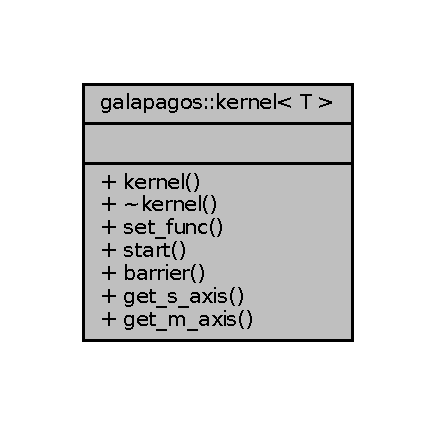
\includegraphics[width=209pt]{classgalapagos_1_1kernel__coll__graph}
\end{center}
\end{figure}
\subsection*{Public Member Functions}
\begin{DoxyCompactItemize}
\item 
\hyperlink{classgalapagos_1_1kernel_a38480cdc220db5649f10288debbf218e}{kernel} (short \+\_\+id)
\item 
\hyperlink{classgalapagos_1_1kernel_a9c36abc6e2c94a2b54a1c00f613dc4d0}{$\sim$kernel} ()
\item 
void \hyperlink{classgalapagos_1_1kernel_ac547afde42a072f87a4afd40e4c094ac}{set\+\_\+func} (void($\ast$\+\_\+func)(short, \hyperlink{classgalapagos_1_1interface}{interface}$<$ \hyperlink{test_8cpp_a0658ceffa730c765d449bb3d21871b5f}{T} $>$ $\ast$, \hyperlink{classgalapagos_1_1interface}{interface}$<$ \hyperlink{test_8cpp_a0658ceffa730c765d449bb3d21871b5f}{T} $>$ $\ast$))
\item 
void \hyperlink{classgalapagos_1_1kernel_a2899d2f4ecda70caa469d367e4ae703d}{start} ()
\item 
void \hyperlink{classgalapagos_1_1kernel_a816fc814f556ff3e9095ab2942cd760a}{barrier} ()
\item 
\hyperlink{classgalapagos_1_1interface}{interface}$<$ \hyperlink{test_8cpp_a0658ceffa730c765d449bb3d21871b5f}{T} $>$ $\ast$ \hyperlink{classgalapagos_1_1kernel_a72b21cb2c96098b694ddee32dfe1e44b}{get\+\_\+s\+\_\+axis} ()
\item 
\hyperlink{classgalapagos_1_1interface}{interface}$<$ \hyperlink{test_8cpp_a0658ceffa730c765d449bb3d21871b5f}{T} $>$ $\ast$ \hyperlink{classgalapagos_1_1kernel_acc4c06e38ca455be99c1a49ce4dbf8d5}{get\+\_\+m\+\_\+axis} ()
\end{DoxyCompactItemize}


\subsection{Detailed Description}
\subsubsection*{template$<$class T$>$\\*
class galapagos\+::kernel$<$ T $>$}

Class for the Kernel wrapper. 

A software wrapper for a kernel object. Wraps an H\+LS synthesizable function and an input interfaces(s\+\_\+axis) and an output interface(m\+\_\+axis). \begin{DoxyAuthor}{Author}
Naif Tarafdar 
\end{DoxyAuthor}
\begin{DoxyDate}{Date}
April 20, 2019 
\end{DoxyDate}


\subsection{Constructor \& Destructor Documentation}
\index{galapagos\+::kernel@{galapagos\+::kernel}!kernel@{kernel}}
\index{kernel@{kernel}!galapagos\+::kernel@{galapagos\+::kernel}}
\subsubsection[{\texorpdfstring{kernel(short \+\_\+id)}{kernel(short _id)}}]{\setlength{\rightskip}{0pt plus 5cm}template$<$class T $>$ {\bf galapagos\+::kernel}$<$ {\bf T} $>$\+::{\bf kernel} (
\begin{DoxyParamCaption}
\item[{short}]{\+\_\+id}
\end{DoxyParamCaption}
)}\hypertarget{classgalapagos_1_1kernel_a38480cdc220db5649f10288debbf218e}{}\label{classgalapagos_1_1kernel_a38480cdc220db5649f10288debbf218e}
\index{galapagos\+::kernel@{galapagos\+::kernel}!````~kernel@{$\sim$kernel}}
\index{````~kernel@{$\sim$kernel}!galapagos\+::kernel@{galapagos\+::kernel}}
\subsubsection[{\texorpdfstring{$\sim$kernel()}{~kernel()}}]{\setlength{\rightskip}{0pt plus 5cm}template$<$class T $>$ {\bf galapagos\+::kernel}$<$ {\bf T} $>$\+::$\sim${\bf kernel} (
\begin{DoxyParamCaption}
{}
\end{DoxyParamCaption}
)\hspace{0.3cm}{\ttfamily [inline]}}\hypertarget{classgalapagos_1_1kernel_a9c36abc6e2c94a2b54a1c00f613dc4d0}{}\label{classgalapagos_1_1kernel_a9c36abc6e2c94a2b54a1c00f613dc4d0}


\subsection{Member Function Documentation}
\index{galapagos\+::kernel@{galapagos\+::kernel}!barrier@{barrier}}
\index{barrier@{barrier}!galapagos\+::kernel@{galapagos\+::kernel}}
\subsubsection[{\texorpdfstring{barrier()}{barrier()}}]{\setlength{\rightskip}{0pt plus 5cm}template$<$class T $>$ void {\bf galapagos\+::kernel}$<$ {\bf T} $>$\+::barrier (
\begin{DoxyParamCaption}
{}
\end{DoxyParamCaption}
)}\hypertarget{classgalapagos_1_1kernel_a816fc814f556ff3e9095ab2942cd760a}{}\label{classgalapagos_1_1kernel_a816fc814f556ff3e9095ab2942cd760a}
Waits for function to finish executing 
\begin{DoxyTemplParams}{Template Parameters}
{\em T} & the type of data used within each galapagos packet (default ap\+\_\+uint$<$64$>$) \\
\hline
\end{DoxyTemplParams}
\index{galapagos\+::kernel@{galapagos\+::kernel}!get\+\_\+m\+\_\+axis@{get\+\_\+m\+\_\+axis}}
\index{get\+\_\+m\+\_\+axis@{get\+\_\+m\+\_\+axis}!galapagos\+::kernel@{galapagos\+::kernel}}
\subsubsection[{\texorpdfstring{get\+\_\+m\+\_\+axis()}{get_m_axis()}}]{\setlength{\rightskip}{0pt plus 5cm}template$<$class T $>$ {\bf galapagos\+::interface}$<$ {\bf T} $>$ $\ast$ {\bf galapagos\+::kernel}$<$ {\bf T} $>$\+::get\+\_\+m\+\_\+axis (
\begin{DoxyParamCaption}
{}
\end{DoxyParamCaption}
)}\hypertarget{classgalapagos_1_1kernel_acc4c06e38ca455be99c1a49ce4dbf8d5}{}\label{classgalapagos_1_1kernel_acc4c06e38ca455be99c1a49ce4dbf8d5}
Gets a pointer to the m\+\_\+axis interface of the kernel 
\begin{DoxyTemplParams}{Template Parameters}
{\em T} & the type of data used within each galapagos packet (default ap\+\_\+uint$<$64$>$) \\
\hline
\end{DoxyTemplParams}
\begin{DoxyReturn}{Returns}
pointer to m\+\_\+axis 
\end{DoxyReturn}
\index{galapagos\+::kernel@{galapagos\+::kernel}!get\+\_\+s\+\_\+axis@{get\+\_\+s\+\_\+axis}}
\index{get\+\_\+s\+\_\+axis@{get\+\_\+s\+\_\+axis}!galapagos\+::kernel@{galapagos\+::kernel}}
\subsubsection[{\texorpdfstring{get\+\_\+s\+\_\+axis()}{get_s_axis()}}]{\setlength{\rightskip}{0pt plus 5cm}template$<$class T $>$ {\bf galapagos\+::interface}$<$ {\bf T} $>$ $\ast$ {\bf galapagos\+::kernel}$<$ {\bf T} $>$\+::get\+\_\+s\+\_\+axis (
\begin{DoxyParamCaption}
{}
\end{DoxyParamCaption}
)}\hypertarget{classgalapagos_1_1kernel_a72b21cb2c96098b694ddee32dfe1e44b}{}\label{classgalapagos_1_1kernel_a72b21cb2c96098b694ddee32dfe1e44b}
Gets a pointer to the s\+\_\+axis interface of the kernel 
\begin{DoxyTemplParams}{Template Parameters}
{\em T} & the type of data used within each galapagos packet (default ap\+\_\+uint$<$64$>$) \\
\hline
\end{DoxyTemplParams}
\begin{DoxyReturn}{Returns}
pointer to s\+\_\+axis 
\end{DoxyReturn}
\index{galapagos\+::kernel@{galapagos\+::kernel}!set\+\_\+func@{set\+\_\+func}}
\index{set\+\_\+func@{set\+\_\+func}!galapagos\+::kernel@{galapagos\+::kernel}}
\subsubsection[{\texorpdfstring{set\+\_\+func(void($\ast$\+\_\+func)(short, interface$<$ T $>$ $\ast$, interface$<$ T $>$ $\ast$))}{set_func(void(*_func)(short, interface< T > *, interface< T > *))}}]{\setlength{\rightskip}{0pt plus 5cm}template$<$class T $>$ void {\bf galapagos\+::kernel}$<$ {\bf T} $>$\+::set\+\_\+func (
\begin{DoxyParamCaption}
\item[{void($\ast$)(short, {\bf interface}$<$ {\bf T} $>$ $\ast$, {\bf interface}$<$ {\bf T} $>$ $\ast$)}]{\+\_\+func}
\end{DoxyParamCaption}
)}\hypertarget{classgalapagos_1_1kernel_ac547afde42a072f87a4afd40e4c094ac}{}\label{classgalapagos_1_1kernel_ac547afde42a072f87a4afd40e4c094ac}
Gives kernel object function pointer of H\+LS synthesizable function to run 
\begin{DoxyTemplParams}{Template Parameters}
{\em T} & the type of data used within each galapagos packet (default ap\+\_\+uint$<$64$>$) \\
\hline
\end{DoxyTemplParams}

\begin{DoxyParams}[1]{Parameters}
\mbox{\tt in}  & {\em \+\_\+func} & function pointer for kernel object to store \\
\hline
\end{DoxyParams}
\index{galapagos\+::kernel@{galapagos\+::kernel}!start@{start}}
\index{start@{start}!galapagos\+::kernel@{galapagos\+::kernel}}
\subsubsection[{\texorpdfstring{start()}{start()}}]{\setlength{\rightskip}{0pt plus 5cm}template$<$class T $>$ void {\bf galapagos\+::kernel}$<$ {\bf T} $>$\+::start (
\begin{DoxyParamCaption}
{}
\end{DoxyParamCaption}
)}\hypertarget{classgalapagos_1_1kernel_a2899d2f4ecda70caa469d367e4ae703d}{}\label{classgalapagos_1_1kernel_a2899d2f4ecda70caa469d367e4ae703d}
Starts function that is being pointed to by kernel 
\begin{DoxyTemplParams}{Template Parameters}
{\em T} & the type of data used within each galapagos packet (default ap\+\_\+uint$<$64$>$) \\
\hline
\end{DoxyTemplParams}


The documentation for this class was generated from the following file\+:\begin{DoxyCompactItemize}
\item 
\hyperlink{galapagos__kernel_8hpp}{galapagos\+\_\+kernel.\+hpp}\end{DoxyCompactItemize}

\hypertarget{classgalapagos_1_1local__router}{}\section{galapagos\+:\+:local\+\_\+router$<$ T $>$ Class Template Reference}
\label{classgalapagos_1_1local__router}\index{galapagos\+::local\+\_\+router$<$ T $>$@{galapagos\+::local\+\_\+router$<$ T $>$}}


Class for the \hyperlink{classgalapagos_1_1local__router}{local\+\_\+router}.  




{\ttfamily \#include $<$galapagos\+\_\+local\+\_\+router.\+hpp$>$}



Collaboration diagram for galapagos\+:\+:local\+\_\+router$<$ T $>$\+:
\nopagebreak
\begin{figure}[H]
\begin{center}
\leavevmode
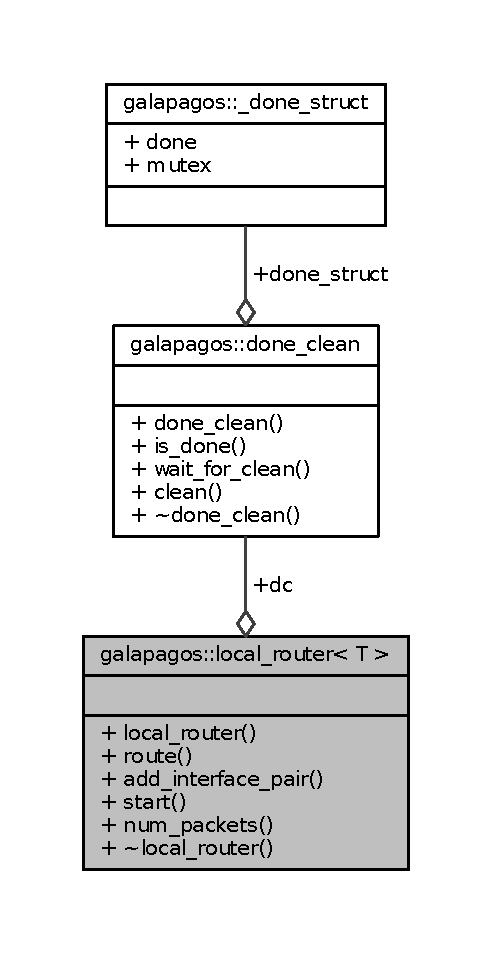
\includegraphics[width=236pt]{classgalapagos_1_1local__router__coll__graph}
\end{center}
\end{figure}
\subsection*{Public Member Functions}
\begin{DoxyCompactItemize}
\item 
\hyperlink{classgalapagos_1_1local__router_a95bf5a1492b589c6ad1c1e5b8126620b}{local\+\_\+router} (std\+::vector$<$ std\+::string $>$ \+\_\+kern\+\_\+info\+\_\+table, std\+::string \+\_\+my\+\_\+address, \hyperlink{classgalapagos_1_1done__clean}{galapagos\+::done\+\_\+clean} $\ast$\+\_\+dc, std\+::mutex $\ast$\+\_\+mutex\+\_\+packets\+\_\+in\+\_\+flight, int $\ast$\+\_\+packets\+\_\+in\+\_\+flight)
\item 
void \hyperlink{classgalapagos_1_1local__router_a339b257abeb779a8809fa1f3cc07098c}{route} ()
\begin{DoxyCompactList}\small\item\em routing function, can be overridden for different routers \end{DoxyCompactList}\item 
void \hyperlink{classgalapagos_1_1local__router_a61fd9df9515ef8ca23708c2cfbead0d3}{add\+\_\+interface\+\_\+pair} (\hyperlink{classgalapagos_1_1interface}{interface}$<$ \hyperlink{test_8cpp_a0658ceffa730c765d449bb3d21871b5f}{T} $>$ $\ast$\+\_\+s\+\_\+axis, \hyperlink{classgalapagos_1_1interface}{interface}$<$ \hyperlink{test_8cpp_a0658ceffa730c765d449bb3d21871b5f}{T} $>$ $\ast$\+\_\+m\+\_\+axis)
\begin{DoxyCompactList}\small\item\em adds a pair of axis interfaces to the router \end{DoxyCompactList}\item 
void \hyperlink{classgalapagos_1_1local__router_a6ad5a95b31f855ba820157ad4439589e}{start} ()
\begin{DoxyCompactList}\small\item\em starts the routing function \end{DoxyCompactList}\item 
unsigned int \hyperlink{classgalapagos_1_1local__router_a3fdc08b885d2166561d1bc43cfe10e4e}{num\+\_\+packets} ()
\begin{DoxyCompactList}\small\item\em returns current number of packets within the router \end{DoxyCompactList}\item 
\hyperlink{classgalapagos_1_1local__router_aabb643170b5f3c8a069e5cbd191a1542}{$\sim$local\+\_\+router} ()
\end{DoxyCompactItemize}
\subsection*{Public Attributes}
\begin{DoxyCompactItemize}
\item 
\hyperlink{classgalapagos_1_1done__clean}{done\+\_\+clean} $\ast$ \hyperlink{classgalapagos_1_1local__router_abb93f7c129e675e8d10bc6a0989a7aba}{dc}
\end{DoxyCompactItemize}


\subsection{Detailed Description}
\subsubsection*{template$<$class T$>$\\*
class galapagos\+::local\+\_\+router$<$ T $>$}

Class for the \hyperlink{classgalapagos_1_1local__router}{local\+\_\+router}. 

A software implementation of the node router, routing packets by dest sidechannel. Routes between input interfaces(s\+\_\+axis) and an output interface(m\+\_\+axis). \begin{DoxyAuthor}{Author}
Naif Tarafdar 
\end{DoxyAuthor}
\begin{DoxyDate}{Date}
April 20, 2019 
\end{DoxyDate}


\subsection{Constructor \& Destructor Documentation}
\index{galapagos\+::local\+\_\+router@{galapagos\+::local\+\_\+router}!local\+\_\+router@{local\+\_\+router}}
\index{local\+\_\+router@{local\+\_\+router}!galapagos\+::local\+\_\+router@{galapagos\+::local\+\_\+router}}
\subsubsection[{\texorpdfstring{local\+\_\+router(std\+::vector$<$ std\+::string $>$ \+\_\+kern\+\_\+info\+\_\+table, std\+::string \+\_\+my\+\_\+address, galapagos\+::done\+\_\+clean $\ast$\+\_\+dc, std\+::mutex $\ast$\+\_\+mutex\+\_\+packets\+\_\+in\+\_\+flight, int $\ast$\+\_\+packets\+\_\+in\+\_\+flight)}{local_router(std::vector< std::string > _kern_info_table, std::string _my_address, galapagos::done_clean *_dc, std::mutex *_mutex_packets_in_flight, int *_packets_in_flight)}}]{\setlength{\rightskip}{0pt plus 5cm}template$<$class T $>$ {\bf galapagos\+::local\+\_\+router}$<$ {\bf T} $>$\+::{\bf local\+\_\+router} (
\begin{DoxyParamCaption}
\item[{std\+::vector$<$ std\+::string $>$}]{\+\_\+kern\+\_\+info\+\_\+table, }
\item[{std\+::string}]{\+\_\+my\+\_\+address, }
\item[{{\bf galapagos\+::done\+\_\+clean} $\ast$}]{\+\_\+dc, }
\item[{std\+::mutex $\ast$}]{\+\_\+mutex\+\_\+packets\+\_\+in\+\_\+flight, }
\item[{int $\ast$}]{\+\_\+packets\+\_\+in\+\_\+flight}
\end{DoxyParamCaption}
)}\hypertarget{classgalapagos_1_1local__router_a95bf5a1492b589c6ad1c1e5b8126620b}{}\label{classgalapagos_1_1local__router_a95bf5a1492b589c6ad1c1e5b8126620b}
\index{galapagos\+::local\+\_\+router@{galapagos\+::local\+\_\+router}!````~local\+\_\+router@{$\sim$local\+\_\+router}}
\index{````~local\+\_\+router@{$\sim$local\+\_\+router}!galapagos\+::local\+\_\+router@{galapagos\+::local\+\_\+router}}
\subsubsection[{\texorpdfstring{$\sim$local\+\_\+router()}{~local_router()}}]{\setlength{\rightskip}{0pt plus 5cm}template$<$class T $>$ {\bf galapagos\+::local\+\_\+router}$<$ {\bf T} $>$\+::$\sim${\bf local\+\_\+router} (
\begin{DoxyParamCaption}
{}
\end{DoxyParamCaption}
)}\hypertarget{classgalapagos_1_1local__router_aabb643170b5f3c8a069e5cbd191a1542}{}\label{classgalapagos_1_1local__router_aabb643170b5f3c8a069e5cbd191a1542}
Local router destructor 
\begin{DoxyTemplParams}{Template Parameters}
{\em T} & the type of data used within each galapagos packet (default ap\+\_\+uint$<$64$>$) \\
\hline
\end{DoxyTemplParams}


\subsection{Member Function Documentation}
\index{galapagos\+::local\+\_\+router@{galapagos\+::local\+\_\+router}!add\+\_\+interface\+\_\+pair@{add\+\_\+interface\+\_\+pair}}
\index{add\+\_\+interface\+\_\+pair@{add\+\_\+interface\+\_\+pair}!galapagos\+::local\+\_\+router@{galapagos\+::local\+\_\+router}}
\subsubsection[{\texorpdfstring{add\+\_\+interface\+\_\+pair(interface$<$ T $>$ $\ast$\+\_\+s\+\_\+axis, interface$<$ T $>$ $\ast$\+\_\+m\+\_\+axis)}{add_interface_pair(interface< T > *_s_axis, interface< T > *_m_axis)}}]{\setlength{\rightskip}{0pt plus 5cm}template$<$class T $>$ void {\bf galapagos\+::local\+\_\+router}$<$ {\bf T} $>$\+::add\+\_\+interface\+\_\+pair (
\begin{DoxyParamCaption}
\item[{{\bf galapagos\+::interface}$<$ {\bf T} $>$ $\ast$}]{\+\_\+s\+\_\+axis, }
\item[{{\bf galapagos\+::interface}$<$ {\bf T} $>$ $\ast$}]{\+\_\+m\+\_\+axis}
\end{DoxyParamCaption}
)}\hypertarget{classgalapagos_1_1local__router_a61fd9df9515ef8ca23708c2cfbead0d3}{}\label{classgalapagos_1_1local__router_a61fd9df9515ef8ca23708c2cfbead0d3}


adds a pair of axis interfaces to the router 

Adds a pair of streaming interfaces to the router 
\begin{DoxyTemplParams}{Template Parameters}
{\em T} & the type of data used within each galapagos packet (default ap\+\_\+uint$<$64$>$) \\
\hline
\end{DoxyTemplParams}

\begin{DoxyParams}[1]{Parameters}
\mbox{\tt in}  & {\em \+\_\+s\+\_\+axis} & input of kernel \\
\hline
\mbox{\tt out}  & {\em \+\_\+m\+\_\+axis} & output of kernel \\
\hline
\end{DoxyParams}
\index{galapagos\+::local\+\_\+router@{galapagos\+::local\+\_\+router}!num\+\_\+packets@{num\+\_\+packets}}
\index{num\+\_\+packets@{num\+\_\+packets}!galapagos\+::local\+\_\+router@{galapagos\+::local\+\_\+router}}
\subsubsection[{\texorpdfstring{num\+\_\+packets()}{num_packets()}}]{\setlength{\rightskip}{0pt plus 5cm}template$<$class T $>$ unsigned int {\bf galapagos\+::local\+\_\+router}$<$ {\bf T} $>$\+::num\+\_\+packets (
\begin{DoxyParamCaption}
{}
\end{DoxyParamCaption}
)}\hypertarget{classgalapagos_1_1local__router_a3fdc08b885d2166561d1bc43cfe10e4e}{}\label{classgalapagos_1_1local__router_a3fdc08b885d2166561d1bc43cfe10e4e}


returns current number of packets within the router 

Returns number of packets within router 
\begin{DoxyTemplParams}{Template Parameters}
{\em T} & the type of data used within each galapagos packet (default ap\+\_\+uint$<$64$>$) \\
\hline
\end{DoxyTemplParams}
\begin{DoxyReturn}{Returns}
number of packets within router 
\end{DoxyReturn}
\index{galapagos\+::local\+\_\+router@{galapagos\+::local\+\_\+router}!route@{route}}
\index{route@{route}!galapagos\+::local\+\_\+router@{galapagos\+::local\+\_\+router}}
\subsubsection[{\texorpdfstring{route()}{route()}}]{\setlength{\rightskip}{0pt plus 5cm}template$<$class T $>$ void {\bf galapagos\+::local\+\_\+router}$<$ {\bf T} $>$\+::route (
\begin{DoxyParamCaption}
{}
\end{DoxyParamCaption}
)}\hypertarget{classgalapagos_1_1local__router_a339b257abeb779a8809fa1f3cc07098c}{}\label{classgalapagos_1_1local__router_a339b257abeb779a8809fa1f3cc07098c}


routing function, can be overridden for different routers 

Routing function Round robins through the m\+\_\+axis (the outputs of all kernels and external drivers). Reads header\+\_\+dest of interface and splices into correct s\+\_\+axis based off dest. This keeps running until the done is asserted externally. 
\begin{DoxyTemplParams}{Template Parameters}
{\em T} & the type of data used within each galapagos packet (default ap\+\_\+uint$<$64$>$) \\
\hline
\end{DoxyTemplParams}
\index{galapagos\+::local\+\_\+router@{galapagos\+::local\+\_\+router}!start@{start}}
\index{start@{start}!galapagos\+::local\+\_\+router@{galapagos\+::local\+\_\+router}}
\subsubsection[{\texorpdfstring{start()}{start()}}]{\setlength{\rightskip}{0pt plus 5cm}template$<$class T $>$ void {\bf galapagos\+::local\+\_\+router}$<$ {\bf T} $>$\+::start (
\begin{DoxyParamCaption}
{}
\end{DoxyParamCaption}
)}\hypertarget{classgalapagos_1_1local__router_a6ad5a95b31f855ba820157ad4439589e}{}\label{classgalapagos_1_1local__router_a6ad5a95b31f855ba820157ad4439589e}


starts the routing function 

Starts the routing function 
\begin{DoxyTemplParams}{Template Parameters}
{\em T} & the type of data used within each galapagos packet (default ap\+\_\+uint$<$64$>$) \\
\hline
\end{DoxyTemplParams}


\subsection{Member Data Documentation}
\index{galapagos\+::local\+\_\+router@{galapagos\+::local\+\_\+router}!dc@{dc}}
\index{dc@{dc}!galapagos\+::local\+\_\+router@{galapagos\+::local\+\_\+router}}
\subsubsection[{\texorpdfstring{dc}{dc}}]{\setlength{\rightskip}{0pt plus 5cm}template$<$class T$>$ {\bf done\+\_\+clean}$\ast$ {\bf galapagos\+::local\+\_\+router}$<$ {\bf T} $>$\+::dc}\hypertarget{classgalapagos_1_1local__router_abb93f7c129e675e8d10bc6a0989a7aba}{}\label{classgalapagos_1_1local__router_abb93f7c129e675e8d10bc6a0989a7aba}


The documentation for this class was generated from the following file\+:\begin{DoxyCompactItemize}
\item 
\hyperlink{galapagos__local__router_8hpp}{galapagos\+\_\+local\+\_\+router.\+hpp}\end{DoxyCompactItemize}

\hypertarget{classmy__barrier}{}\section{my\+\_\+barrier Class Reference}
\label{classmy__barrier}\index{my\+\_\+barrier@{my\+\_\+barrier}}


Collaboration diagram for my\+\_\+barrier\+:
\nopagebreak
\begin{figure}[H]
\begin{center}
\leavevmode
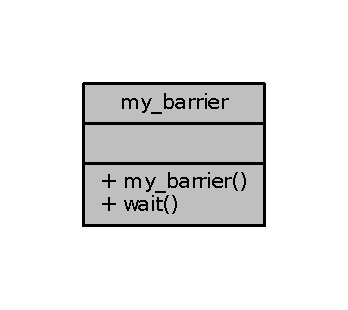
\includegraphics[width=167pt]{classmy__barrier__coll__graph}
\end{center}
\end{figure}
\subsection*{Public Member Functions}
\begin{DoxyCompactItemize}
\item 
\hyperlink{classmy__barrier_a4bdc21169a5627bb2dd4cf7a3a28087e}{my\+\_\+barrier} (int count)
\item 
void \hyperlink{classmy__barrier_aecfdacf9fe1400cc2f2917d5e760b794}{wait} ()
\end{DoxyCompactItemize}


\subsection{Constructor \& Destructor Documentation}
\index{my\+\_\+barrier@{my\+\_\+barrier}!my\+\_\+barrier@{my\+\_\+barrier}}
\index{my\+\_\+barrier@{my\+\_\+barrier}!my\+\_\+barrier@{my\+\_\+barrier}}
\subsubsection[{\texorpdfstring{my\+\_\+barrier(int count)}{my_barrier(int count)}}]{\setlength{\rightskip}{0pt plus 5cm}my\+\_\+barrier\+::my\+\_\+barrier (
\begin{DoxyParamCaption}
\item[{int}]{count}
\end{DoxyParamCaption}
)\hspace{0.3cm}{\ttfamily [inline]}}\hypertarget{classmy__barrier_a4bdc21169a5627bb2dd4cf7a3a28087e}{}\label{classmy__barrier_a4bdc21169a5627bb2dd4cf7a3a28087e}


\subsection{Member Function Documentation}
\index{my\+\_\+barrier@{my\+\_\+barrier}!wait@{wait}}
\index{wait@{wait}!my\+\_\+barrier@{my\+\_\+barrier}}
\subsubsection[{\texorpdfstring{wait()}{wait()}}]{\setlength{\rightskip}{0pt plus 5cm}void my\+\_\+barrier\+::wait (
\begin{DoxyParamCaption}
{}
\end{DoxyParamCaption}
)\hspace{0.3cm}{\ttfamily [inline]}}\hypertarget{classmy__barrier_aecfdacf9fe1400cc2f2917d5e760b794}{}\label{classmy__barrier_aecfdacf9fe1400cc2f2917d5e760b794}


The documentation for this class was generated from the following file\+:\begin{DoxyCompactItemize}
\item 
\hyperlink{benchmark__0_8cpp}{benchmark\+\_\+0.\+cpp}\end{DoxyCompactItemize}

\hypertarget{classgalapagos_1_1n__to__one__router}{}\section{galapagos\+:\+:n\+\_\+to\+\_\+one\+\_\+router$<$ T $>$ Class Template Reference}
\label{classgalapagos_1_1n__to__one__router}\index{galapagos\+::n\+\_\+to\+\_\+one\+\_\+router$<$ T $>$@{galapagos\+::n\+\_\+to\+\_\+one\+\_\+router$<$ T $>$}}


Class for the \hyperlink{classgalapagos_1_1n__to__one__router}{n\+\_\+to\+\_\+one\+\_\+router}.  




{\ttfamily \#include $<$galapagos\+\_\+n\+\_\+to\+\_\+one\+\_\+router.\+hpp$>$}



Collaboration diagram for galapagos\+:\+:n\+\_\+to\+\_\+one\+\_\+router$<$ T $>$\+:
\nopagebreak
\begin{figure}[H]
\begin{center}
\leavevmode
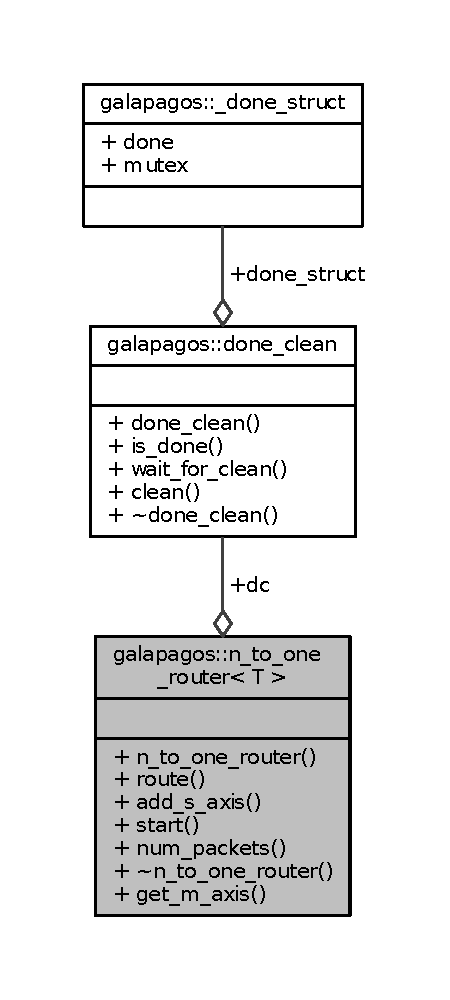
\includegraphics[width=216pt]{classgalapagos_1_1n__to__one__router__coll__graph}
\end{center}
\end{figure}
\subsection*{Public Member Functions}
\begin{DoxyCompactItemize}
\item 
\hyperlink{classgalapagos_1_1n__to__one__router_a3fbff119ec60336ceb9b4211da7390c8}{n\+\_\+to\+\_\+one\+\_\+router} (\hyperlink{classgalapagos_1_1done__clean}{done\+\_\+clean} $\ast$\+\_\+dc)
\item 
void \hyperlink{classgalapagos_1_1n__to__one__router_ae4d5a405ad2706d909fd8b261b2ee7f9}{route} ()
\begin{DoxyCompactList}\small\item\em routing function, can be overridden for different routers \end{DoxyCompactList}\item 
void \hyperlink{classgalapagos_1_1n__to__one__router_a9f20fa4aaa47b5aceb838fc19e468854}{add\+\_\+s\+\_\+axis} (\hyperlink{classgalapagos_1_1interface}{interface}$<$ \hyperlink{test_8cpp_a0658ceffa730c765d449bb3d21871b5f}{T} $>$ $\ast$\+\_\+s\+\_\+axis)
\begin{DoxyCompactList}\small\item\em adds a pair of axis interfaces to the router \end{DoxyCompactList}\item 
void \hyperlink{classgalapagos_1_1n__to__one__router_afc25a84a3b345401a91b1c2b7c8484ae}{start} ()
\begin{DoxyCompactList}\small\item\em starts the routing function \end{DoxyCompactList}\item 
unsigned int \hyperlink{classgalapagos_1_1n__to__one__router_ae79a9ee609e42b91f3e8058a0a24fc0c}{num\+\_\+packets} ()
\begin{DoxyCompactList}\small\item\em returns current number of packets within the router \end{DoxyCompactList}\item 
\hyperlink{classgalapagos_1_1n__to__one__router_a1b38ec16587aaa2e3d56ffa5c9afa008}{$\sim$n\+\_\+to\+\_\+one\+\_\+router} ()
\item 
\hyperlink{classgalapagos_1_1interface}{interface}$<$ \hyperlink{test_8cpp_a0658ceffa730c765d449bb3d21871b5f}{T} $>$ $\ast$ \hyperlink{classgalapagos_1_1n__to__one__router_a65b746fb4a20c0260a3b93af0a907be6}{get\+\_\+m\+\_\+axis} ()
\end{DoxyCompactItemize}
\subsection*{Public Attributes}
\begin{DoxyCompactItemize}
\item 
\hyperlink{classgalapagos_1_1done__clean}{done\+\_\+clean} $\ast$ \hyperlink{classgalapagos_1_1n__to__one__router_a42603cc4ee2ee8391a7d0e14bb1f39df}{dc}
\end{DoxyCompactItemize}


\subsection{Detailed Description}
\subsubsection*{template$<$class T$>$\\*
class galapagos\+::n\+\_\+to\+\_\+one\+\_\+router$<$ T $>$}

Class for the \hyperlink{classgalapagos_1_1n__to__one__router}{n\+\_\+to\+\_\+one\+\_\+router}. 

A software implementation of an n to one router, used by network node to arbitrade output of sessions into the node. Routes between input interfaces(s\+\_\+axis) and an output interface(m\+\_\+axis). \begin{DoxyAuthor}{Author}
Naif Tarafdar 
\end{DoxyAuthor}
\begin{DoxyDate}{Date}
April 20, 2019 
\end{DoxyDate}


\subsection{Constructor \& Destructor Documentation}
\index{galapagos\+::n\+\_\+to\+\_\+one\+\_\+router@{galapagos\+::n\+\_\+to\+\_\+one\+\_\+router}!n\+\_\+to\+\_\+one\+\_\+router@{n\+\_\+to\+\_\+one\+\_\+router}}
\index{n\+\_\+to\+\_\+one\+\_\+router@{n\+\_\+to\+\_\+one\+\_\+router}!galapagos\+::n\+\_\+to\+\_\+one\+\_\+router@{galapagos\+::n\+\_\+to\+\_\+one\+\_\+router}}
\subsubsection[{\texorpdfstring{n\+\_\+to\+\_\+one\+\_\+router(done\+\_\+clean $\ast$\+\_\+dc)}{n_to_one_router(done_clean *_dc)}}]{\setlength{\rightskip}{0pt plus 5cm}template$<$class T $>$ {\bf galapagos\+::n\+\_\+to\+\_\+one\+\_\+router}$<$ {\bf T} $>$\+::{\bf n\+\_\+to\+\_\+one\+\_\+router} (
\begin{DoxyParamCaption}
\item[{{\bf done\+\_\+clean} $\ast$}]{\+\_\+dc}
\end{DoxyParamCaption}
)}\hypertarget{classgalapagos_1_1n__to__one__router_a3fbff119ec60336ceb9b4211da7390c8}{}\label{classgalapagos_1_1n__to__one__router_a3fbff119ec60336ceb9b4211da7390c8}
\index{galapagos\+::n\+\_\+to\+\_\+one\+\_\+router@{galapagos\+::n\+\_\+to\+\_\+one\+\_\+router}!````~n\+\_\+to\+\_\+one\+\_\+router@{$\sim$n\+\_\+to\+\_\+one\+\_\+router}}
\index{````~n\+\_\+to\+\_\+one\+\_\+router@{$\sim$n\+\_\+to\+\_\+one\+\_\+router}!galapagos\+::n\+\_\+to\+\_\+one\+\_\+router@{galapagos\+::n\+\_\+to\+\_\+one\+\_\+router}}
\subsubsection[{\texorpdfstring{$\sim$n\+\_\+to\+\_\+one\+\_\+router()}{~n_to_one_router()}}]{\setlength{\rightskip}{0pt plus 5cm}template$<$class T $>$ {\bf galapagos\+::n\+\_\+to\+\_\+one\+\_\+router}$<$ {\bf T} $>$\+::$\sim${\bf n\+\_\+to\+\_\+one\+\_\+router} (
\begin{DoxyParamCaption}
{}
\end{DoxyParamCaption}
)}\hypertarget{classgalapagos_1_1n__to__one__router_a1b38ec16587aaa2e3d56ffa5c9afa008}{}\label{classgalapagos_1_1n__to__one__router_a1b38ec16587aaa2e3d56ffa5c9afa008}
n to one destructor 
\begin{DoxyTemplParams}{Template Parameters}
{\em T} & the type of data used within each galapagos packet (default ap\+\_\+uint$<$64$>$) \\
\hline
\end{DoxyTemplParams}


\subsection{Member Function Documentation}
\index{galapagos\+::n\+\_\+to\+\_\+one\+\_\+router@{galapagos\+::n\+\_\+to\+\_\+one\+\_\+router}!add\+\_\+s\+\_\+axis@{add\+\_\+s\+\_\+axis}}
\index{add\+\_\+s\+\_\+axis@{add\+\_\+s\+\_\+axis}!galapagos\+::n\+\_\+to\+\_\+one\+\_\+router@{galapagos\+::n\+\_\+to\+\_\+one\+\_\+router}}
\subsubsection[{\texorpdfstring{add\+\_\+s\+\_\+axis(interface$<$ T $>$ $\ast$\+\_\+s\+\_\+axis)}{add_s_axis(interface< T > *_s_axis)}}]{\setlength{\rightskip}{0pt plus 5cm}template$<$class T $>$ void {\bf galapagos\+::n\+\_\+to\+\_\+one\+\_\+router}$<$ {\bf T} $>$\+::add\+\_\+s\+\_\+axis (
\begin{DoxyParamCaption}
\item[{{\bf galapagos\+::interface}$<$ {\bf T} $>$ $\ast$}]{\+\_\+s\+\_\+axis}
\end{DoxyParamCaption}
)}\hypertarget{classgalapagos_1_1n__to__one__router_a9f20fa4aaa47b5aceb838fc19e468854}{}\label{classgalapagos_1_1n__to__one__router_a9f20fa4aaa47b5aceb838fc19e468854}


adds a pair of axis interfaces to the router 

Adds a new interface to the list of inputs 
\begin{DoxyTemplParams}{Template Parameters}
{\em T} & the type of data used within each galapagos packet (default ap\+\_\+uint$<$64$>$) \\
\hline
\end{DoxyTemplParams}

\begin{DoxyParams}[1]{Parameters}
\mbox{\tt in}  & {\em \+\_\+s\+\_\+axis} & interface to add to list \\
\hline
\end{DoxyParams}
\index{galapagos\+::n\+\_\+to\+\_\+one\+\_\+router@{galapagos\+::n\+\_\+to\+\_\+one\+\_\+router}!get\+\_\+m\+\_\+axis@{get\+\_\+m\+\_\+axis}}
\index{get\+\_\+m\+\_\+axis@{get\+\_\+m\+\_\+axis}!galapagos\+::n\+\_\+to\+\_\+one\+\_\+router@{galapagos\+::n\+\_\+to\+\_\+one\+\_\+router}}
\subsubsection[{\texorpdfstring{get\+\_\+m\+\_\+axis()}{get_m_axis()}}]{\setlength{\rightskip}{0pt plus 5cm}template$<$class T $>$ {\bf galapagos\+::interface}$<$ {\bf T} $>$ $\ast$ {\bf galapagos\+::n\+\_\+to\+\_\+one\+\_\+router}$<$ {\bf T} $>$\+::get\+\_\+m\+\_\+axis (
\begin{DoxyParamCaption}
{}
\end{DoxyParamCaption}
)}\hypertarget{classgalapagos_1_1n__to__one__router_a65b746fb4a20c0260a3b93af0a907be6}{}\label{classgalapagos_1_1n__to__one__router_a65b746fb4a20c0260a3b93af0a907be6}
\index{galapagos\+::n\+\_\+to\+\_\+one\+\_\+router@{galapagos\+::n\+\_\+to\+\_\+one\+\_\+router}!num\+\_\+packets@{num\+\_\+packets}}
\index{num\+\_\+packets@{num\+\_\+packets}!galapagos\+::n\+\_\+to\+\_\+one\+\_\+router@{galapagos\+::n\+\_\+to\+\_\+one\+\_\+router}}
\subsubsection[{\texorpdfstring{num\+\_\+packets()}{num_packets()}}]{\setlength{\rightskip}{0pt plus 5cm}template$<$class T $>$ unsigned int {\bf galapagos\+::n\+\_\+to\+\_\+one\+\_\+router}$<$ {\bf T} $>$\+::num\+\_\+packets (
\begin{DoxyParamCaption}
{}
\end{DoxyParamCaption}
)}\hypertarget{classgalapagos_1_1n__to__one__router_ae79a9ee609e42b91f3e8058a0a24fc0c}{}\label{classgalapagos_1_1n__to__one__router_ae79a9ee609e42b91f3e8058a0a24fc0c}


returns current number of packets within the router 

Returns number of packets within router 
\begin{DoxyTemplParams}{Template Parameters}
{\em T} & the type of data used within each galapagos packet (default ap\+\_\+uint$<$64$>$) \\
\hline
\end{DoxyTemplParams}
\begin{DoxyReturn}{Returns}
number of packets within router 
\end{DoxyReturn}
\index{galapagos\+::n\+\_\+to\+\_\+one\+\_\+router@{galapagos\+::n\+\_\+to\+\_\+one\+\_\+router}!route@{route}}
\index{route@{route}!galapagos\+::n\+\_\+to\+\_\+one\+\_\+router@{galapagos\+::n\+\_\+to\+\_\+one\+\_\+router}}
\subsubsection[{\texorpdfstring{route()}{route()}}]{\setlength{\rightskip}{0pt plus 5cm}template$<$class T $>$ void {\bf galapagos\+::n\+\_\+to\+\_\+one\+\_\+router}$<$ {\bf T} $>$\+::route (
\begin{DoxyParamCaption}
{}
\end{DoxyParamCaption}
)}\hypertarget{classgalapagos_1_1n__to__one__router_ae4d5a405ad2706d909fd8b261b2ee7f9}{}\label{classgalapagos_1_1n__to__one__router_ae4d5a405ad2706d909fd8b261b2ee7f9}


routing function, can be overridden for different routers 

Routing function Round robins through the m\+\_\+axis (the outputs of all kernels and external drivers). Reads header\+\_\+dest of interface and splices into correct s\+\_\+axis based off dest. This keeps running until the done is asserted externally. 
\begin{DoxyTemplParams}{Template Parameters}
{\em T} & the type of data used within each galapagos packet (default ap\+\_\+uint$<$64$>$) \\
\hline
\end{DoxyTemplParams}
\index{galapagos\+::n\+\_\+to\+\_\+one\+\_\+router@{galapagos\+::n\+\_\+to\+\_\+one\+\_\+router}!start@{start}}
\index{start@{start}!galapagos\+::n\+\_\+to\+\_\+one\+\_\+router@{galapagos\+::n\+\_\+to\+\_\+one\+\_\+router}}
\subsubsection[{\texorpdfstring{start()}{start()}}]{\setlength{\rightskip}{0pt plus 5cm}template$<$class T $>$ void {\bf galapagos\+::n\+\_\+to\+\_\+one\+\_\+router}$<$ {\bf T} $>$\+::start (
\begin{DoxyParamCaption}
{}
\end{DoxyParamCaption}
)}\hypertarget{classgalapagos_1_1n__to__one__router_afc25a84a3b345401a91b1c2b7c8484ae}{}\label{classgalapagos_1_1n__to__one__router_afc25a84a3b345401a91b1c2b7c8484ae}


starts the routing function 

Starts the routing function 
\begin{DoxyTemplParams}{Template Parameters}
{\em T} & the type of data used within each galapagos packet (default ap\+\_\+uint$<$64$>$) \\
\hline
\end{DoxyTemplParams}


\subsection{Member Data Documentation}
\index{galapagos\+::n\+\_\+to\+\_\+one\+\_\+router@{galapagos\+::n\+\_\+to\+\_\+one\+\_\+router}!dc@{dc}}
\index{dc@{dc}!galapagos\+::n\+\_\+to\+\_\+one\+\_\+router@{galapagos\+::n\+\_\+to\+\_\+one\+\_\+router}}
\subsubsection[{\texorpdfstring{dc}{dc}}]{\setlength{\rightskip}{0pt plus 5cm}template$<$class T$>$ {\bf done\+\_\+clean}$\ast$ {\bf galapagos\+::n\+\_\+to\+\_\+one\+\_\+router}$<$ {\bf T} $>$\+::dc}\hypertarget{classgalapagos_1_1n__to__one__router_a42603cc4ee2ee8391a7d0e14bb1f39df}{}\label{classgalapagos_1_1n__to__one__router_a42603cc4ee2ee8391a7d0e14bb1f39df}


The documentation for this class was generated from the following file\+:\begin{DoxyCompactItemize}
\item 
\hyperlink{galapagos__n__to__one__router_8hpp}{galapagos\+\_\+n\+\_\+to\+\_\+one\+\_\+router.\+hpp}\end{DoxyCompactItemize}

\hypertarget{classgalapagos_1_1node}{}\section{galapagos\+:\+:node$<$ T $>$ Class Template Reference}
\label{classgalapagos_1_1node}\index{galapagos\+::node$<$ T $>$@{galapagos\+::node$<$ T $>$}}


{\ttfamily \#include $<$galapagos\+\_\+node.\+hpp$>$}



Collaboration diagram for galapagos\+:\+:node$<$ T $>$\+:
\nopagebreak
\begin{figure}[H]
\begin{center}
\leavevmode
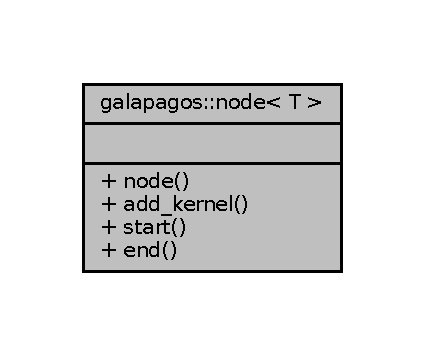
\includegraphics[width=204pt]{classgalapagos_1_1node__coll__graph}
\end{center}
\end{figure}
\subsection*{Public Member Functions}
\begin{DoxyCompactItemize}
\item 
\hyperlink{classgalapagos_1_1node_a7cb6e9d7b42bce3052214e7256408bfd}{node} (std\+::vector$<$ std\+::string $>$ \+\_\+kern\+\_\+info\+\_\+table, std\+::string \+\_\+my\+\_\+address, std\+::vector$<$ \hyperlink{classgalapagos_1_1external__driver}{galapagos\+::external\+\_\+driver}$<$ \hyperlink{test_8cpp_a0658ceffa730c765d449bb3d21871b5f}{T} $>$ $\ast$ $>$ \+\_\+ext\+\_\+drivers)
\item 
void \hyperlink{classgalapagos_1_1node_a085cc57860935c281c396d9b03ee0e41}{add\+\_\+kernel} (short id, void($\ast$func)(short, \hyperlink{classgalapagos_1_1interface}{interface}$<$ \hyperlink{test_8cpp_a0658ceffa730c765d449bb3d21871b5f}{T} $>$ $\ast$, \hyperlink{classgalapagos_1_1interface}{interface}$<$ \hyperlink{test_8cpp_a0658ceffa730c765d449bb3d21871b5f}{T} $>$ $\ast$))
\item 
void \hyperlink{classgalapagos_1_1node_a867d21a2e0f0c83cada0cc2ac8ee4d00}{start} ()
\item 
void \hyperlink{classgalapagos_1_1node_a919af41e5ac382cea85899fbc9084bb3}{end} ()
\end{DoxyCompactItemize}


\subsection{Constructor \& Destructor Documentation}
\index{galapagos\+::node@{galapagos\+::node}!node@{node}}
\index{node@{node}!galapagos\+::node@{galapagos\+::node}}
\subsubsection[{\texorpdfstring{node(std\+::vector$<$ std\+::string $>$ \+\_\+kern\+\_\+info\+\_\+table, std\+::string \+\_\+my\+\_\+address, std\+::vector$<$ galapagos\+::external\+\_\+driver$<$ T $>$ $\ast$ $>$ \+\_\+ext\+\_\+drivers)}{node(std::vector< std::string > _kern_info_table, std::string _my_address, std::vector< galapagos::external_driver< T > * > _ext_drivers)}}]{\setlength{\rightskip}{0pt plus 5cm}template$<$class T $>$ {\bf galapagos\+::node}$<$ {\bf T} $>$\+::{\bf node} (
\begin{DoxyParamCaption}
\item[{std\+::vector$<$ std\+::string $>$}]{\+\_\+kern\+\_\+info\+\_\+table, }
\item[{std\+::string}]{\+\_\+my\+\_\+address, }
\item[{std\+::vector$<$ {\bf galapagos\+::external\+\_\+driver}$<$ {\bf T} $>$ $\ast$ $>$}]{\+\_\+ext\+\_\+drivers}
\end{DoxyParamCaption}
)}\hypertarget{classgalapagos_1_1node_a7cb6e9d7b42bce3052214e7256408bfd}{}\label{classgalapagos_1_1node_a7cb6e9d7b42bce3052214e7256408bfd}


\subsection{Member Function Documentation}
\index{galapagos\+::node@{galapagos\+::node}!add\+\_\+kernel@{add\+\_\+kernel}}
\index{add\+\_\+kernel@{add\+\_\+kernel}!galapagos\+::node@{galapagos\+::node}}
\subsubsection[{\texorpdfstring{add\+\_\+kernel(short id, void($\ast$func)(short, interface$<$ T $>$ $\ast$, interface$<$ T $>$ $\ast$))}{add_kernel(short id, void(*func)(short, interface< T > *, interface< T > *))}}]{\setlength{\rightskip}{0pt plus 5cm}template$<$class T $>$ void {\bf galapagos\+::node}$<$ {\bf T} $>$\+::add\+\_\+kernel (
\begin{DoxyParamCaption}
\item[{short}]{id, }
\item[{void($\ast$)(short, {\bf interface}$<$ {\bf T} $>$ $\ast$, {\bf interface}$<$ {\bf T} $>$ $\ast$)}]{func}
\end{DoxyParamCaption}
)}\hypertarget{classgalapagos_1_1node_a085cc57860935c281c396d9b03ee0e41}{}\label{classgalapagos_1_1node_a085cc57860935c281c396d9b03ee0e41}
\index{galapagos\+::node@{galapagos\+::node}!end@{end}}
\index{end@{end}!galapagos\+::node@{galapagos\+::node}}
\subsubsection[{\texorpdfstring{end()}{end()}}]{\setlength{\rightskip}{0pt plus 5cm}template$<$class T $>$ void {\bf galapagos\+::node}$<$ {\bf T} $>$\+::end (
\begin{DoxyParamCaption}
{}
\end{DoxyParamCaption}
)}\hypertarget{classgalapagos_1_1node_a919af41e5ac382cea85899fbc9084bb3}{}\label{classgalapagos_1_1node_a919af41e5ac382cea85899fbc9084bb3}
\index{galapagos\+::node@{galapagos\+::node}!start@{start}}
\index{start@{start}!galapagos\+::node@{galapagos\+::node}}
\subsubsection[{\texorpdfstring{start()}{start()}}]{\setlength{\rightskip}{0pt plus 5cm}template$<$class T $>$ void {\bf galapagos\+::node}$<$ {\bf T} $>$\+::start (
\begin{DoxyParamCaption}
{}
\end{DoxyParamCaption}
)}\hypertarget{classgalapagos_1_1node_a867d21a2e0f0c83cada0cc2ac8ee4d00}{}\label{classgalapagos_1_1node_a867d21a2e0f0c83cada0cc2ac8ee4d00}


The documentation for this class was generated from the following file\+:\begin{DoxyCompactItemize}
\item 
\hyperlink{galapagos__node_8hpp}{galapagos\+\_\+node.\+hpp}\end{DoxyCompactItemize}

\hypertarget{structgalapagos_1_1stream__packet}{}\section{galapagos\+:\+:stream\+\_\+packet$<$ T $>$ Struct Template Reference}
\label{structgalapagos_1_1stream__packet}\index{galapagos\+::stream\+\_\+packet$<$ T $>$@{galapagos\+::stream\+\_\+packet$<$ T $>$}}


{\ttfamily \#include $<$galapagos\+\_\+packet.\+h$>$}



Collaboration diagram for galapagos\+:\+:stream\+\_\+packet$<$ T $>$\+:
\nopagebreak
\begin{figure}[H]
\begin{center}
\leavevmode
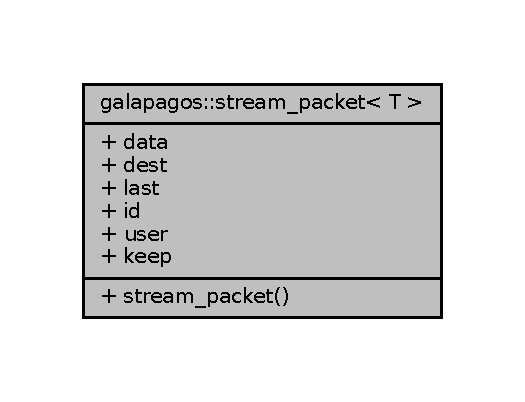
\includegraphics[width=252pt]{structgalapagos_1_1stream__packet__coll__graph}
\end{center}
\end{figure}
\subsection*{Public Member Functions}
\begin{DoxyCompactItemize}
\item 
\hyperlink{structgalapagos_1_1stream__packet_af46f1b60d18aee3839505b109c9321a5}{stream\+\_\+packet} ()
\end{DoxyCompactItemize}
\subsection*{Public Attributes}
\begin{DoxyCompactItemize}
\item 
\hyperlink{test_8cpp_a0658ceffa730c765d449bb3d21871b5f}{T} \hyperlink{structgalapagos_1_1stream__packet_ab7df62196ecabd5c8a84b626653ce053}{data}
\item 
ap\+\_\+uint$<$ \hyperlink{packet__size_8h_a5e007ff81bb2779243ac4d9984a00dff}{P\+A\+C\+K\+E\+T\+\_\+\+D\+E\+S\+T\+\_\+\+L\+E\+N\+G\+TH} $>$ \hyperlink{structgalapagos_1_1stream__packet_a02e87b0b9321904135595e35e3df5c3e}{dest}
\item 
ap\+\_\+uint$<$ 1 $>$ \hyperlink{structgalapagos_1_1stream__packet_ac24df7348558cf3c41f925ca06d47df6}{last}
\item 
ap\+\_\+uint$<$ \hyperlink{packet__size_8h_a5e007ff81bb2779243ac4d9984a00dff}{P\+A\+C\+K\+E\+T\+\_\+\+D\+E\+S\+T\+\_\+\+L\+E\+N\+G\+TH} $>$ \hyperlink{structgalapagos_1_1stream__packet_a0a24dc38c3b6df8b686af2873d6c997d}{id}
\item 
ap\+\_\+uint$<$ \hyperlink{packet__size_8h_af5db3d603be0d574545c417ad0e0520d}{P\+A\+C\+K\+E\+T\+\_\+\+U\+S\+E\+R\+\_\+\+L\+E\+N\+G\+TH} $>$ \hyperlink{structgalapagos_1_1stream__packet_a2907d53b45fb3a8d84f3dc5258994e96}{user}
\item 
ap\+\_\+uint$<$ \hyperlink{packet__size_8h_aee5508cfda1787ded27d89e65f433082}{P\+A\+C\+K\+E\+T\+\_\+\+K\+E\+E\+P\+\_\+\+L\+E\+N\+G\+TH} $>$ \hyperlink{structgalapagos_1_1stream__packet_af69cb752aebbfc03ef33c571a08e1b55}{keep}
\end{DoxyCompactItemize}


\subsection{Constructor \& Destructor Documentation}
\index{galapagos\+::stream\+\_\+packet@{galapagos\+::stream\+\_\+packet}!stream\+\_\+packet@{stream\+\_\+packet}}
\index{stream\+\_\+packet@{stream\+\_\+packet}!galapagos\+::stream\+\_\+packet@{galapagos\+::stream\+\_\+packet}}
\subsubsection[{\texorpdfstring{stream\+\_\+packet()}{stream_packet()}}]{\setlength{\rightskip}{0pt plus 5cm}template$<$typename T$>$ {\bf galapagos\+::stream\+\_\+packet}$<$ {\bf T} $>$\+::{\bf stream\+\_\+packet} (
\begin{DoxyParamCaption}
{}
\end{DoxyParamCaption}
)\hspace{0.3cm}{\ttfamily [inline]}}\hypertarget{structgalapagos_1_1stream__packet_af46f1b60d18aee3839505b109c9321a5}{}\label{structgalapagos_1_1stream__packet_af46f1b60d18aee3839505b109c9321a5}


\subsection{Member Data Documentation}
\index{galapagos\+::stream\+\_\+packet@{galapagos\+::stream\+\_\+packet}!data@{data}}
\index{data@{data}!galapagos\+::stream\+\_\+packet@{galapagos\+::stream\+\_\+packet}}
\subsubsection[{\texorpdfstring{data}{data}}]{\setlength{\rightskip}{0pt plus 5cm}template$<$typename T$>$ {\bf T} {\bf galapagos\+::stream\+\_\+packet}$<$ {\bf T} $>$\+::data}\hypertarget{structgalapagos_1_1stream__packet_ab7df62196ecabd5c8a84b626653ce053}{}\label{structgalapagos_1_1stream__packet_ab7df62196ecabd5c8a84b626653ce053}
\index{galapagos\+::stream\+\_\+packet@{galapagos\+::stream\+\_\+packet}!dest@{dest}}
\index{dest@{dest}!galapagos\+::stream\+\_\+packet@{galapagos\+::stream\+\_\+packet}}
\subsubsection[{\texorpdfstring{dest}{dest}}]{\setlength{\rightskip}{0pt plus 5cm}template$<$typename T$>$ ap\+\_\+uint$<${\bf P\+A\+C\+K\+E\+T\+\_\+\+D\+E\+S\+T\+\_\+\+L\+E\+N\+G\+TH}$>$ {\bf galapagos\+::stream\+\_\+packet}$<$ {\bf T} $>$\+::dest}\hypertarget{structgalapagos_1_1stream__packet_a02e87b0b9321904135595e35e3df5c3e}{}\label{structgalapagos_1_1stream__packet_a02e87b0b9321904135595e35e3df5c3e}
\index{galapagos\+::stream\+\_\+packet@{galapagos\+::stream\+\_\+packet}!id@{id}}
\index{id@{id}!galapagos\+::stream\+\_\+packet@{galapagos\+::stream\+\_\+packet}}
\subsubsection[{\texorpdfstring{id}{id}}]{\setlength{\rightskip}{0pt plus 5cm}template$<$typename T$>$ ap\+\_\+uint$<${\bf P\+A\+C\+K\+E\+T\+\_\+\+D\+E\+S\+T\+\_\+\+L\+E\+N\+G\+TH}$>$ {\bf galapagos\+::stream\+\_\+packet}$<$ {\bf T} $>$\+::id}\hypertarget{structgalapagos_1_1stream__packet_a0a24dc38c3b6df8b686af2873d6c997d}{}\label{structgalapagos_1_1stream__packet_a0a24dc38c3b6df8b686af2873d6c997d}
\index{galapagos\+::stream\+\_\+packet@{galapagos\+::stream\+\_\+packet}!keep@{keep}}
\index{keep@{keep}!galapagos\+::stream\+\_\+packet@{galapagos\+::stream\+\_\+packet}}
\subsubsection[{\texorpdfstring{keep}{keep}}]{\setlength{\rightskip}{0pt plus 5cm}template$<$typename T$>$ ap\+\_\+uint$<${\bf P\+A\+C\+K\+E\+T\+\_\+\+K\+E\+E\+P\+\_\+\+L\+E\+N\+G\+TH}$>$ {\bf galapagos\+::stream\+\_\+packet}$<$ {\bf T} $>$\+::keep}\hypertarget{structgalapagos_1_1stream__packet_af69cb752aebbfc03ef33c571a08e1b55}{}\label{structgalapagos_1_1stream__packet_af69cb752aebbfc03ef33c571a08e1b55}
\index{galapagos\+::stream\+\_\+packet@{galapagos\+::stream\+\_\+packet}!last@{last}}
\index{last@{last}!galapagos\+::stream\+\_\+packet@{galapagos\+::stream\+\_\+packet}}
\subsubsection[{\texorpdfstring{last}{last}}]{\setlength{\rightskip}{0pt plus 5cm}template$<$typename T$>$ ap\+\_\+uint$<$1$>$ {\bf galapagos\+::stream\+\_\+packet}$<$ {\bf T} $>$\+::last}\hypertarget{structgalapagos_1_1stream__packet_ac24df7348558cf3c41f925ca06d47df6}{}\label{structgalapagos_1_1stream__packet_ac24df7348558cf3c41f925ca06d47df6}
\index{galapagos\+::stream\+\_\+packet@{galapagos\+::stream\+\_\+packet}!user@{user}}
\index{user@{user}!galapagos\+::stream\+\_\+packet@{galapagos\+::stream\+\_\+packet}}
\subsubsection[{\texorpdfstring{user}{user}}]{\setlength{\rightskip}{0pt plus 5cm}template$<$typename T$>$ ap\+\_\+uint$<${\bf P\+A\+C\+K\+E\+T\+\_\+\+U\+S\+E\+R\+\_\+\+L\+E\+N\+G\+TH}$>$ {\bf galapagos\+::stream\+\_\+packet}$<$ {\bf T} $>$\+::user}\hypertarget{structgalapagos_1_1stream__packet_a2907d53b45fb3a8d84f3dc5258994e96}{}\label{structgalapagos_1_1stream__packet_a2907d53b45fb3a8d84f3dc5258994e96}


The documentation for this struct was generated from the following file\+:\begin{DoxyCompactItemize}
\item 
\hyperlink{galapagos__packet_8h}{galapagos\+\_\+packet.\+h}\end{DoxyCompactItemize}

\hypertarget{classgalapagos_1_1net_1_1tcp}{}\section{galapagos\+:\+:net\+:\+:tcp$<$ T $>$ Class Template Reference}
\label{classgalapagos_1_1net_1_1tcp}\index{galapagos\+::net\+::tcp$<$ T $>$@{galapagos\+::net\+::tcp$<$ T $>$}}


Class tcp driver.  




{\ttfamily \#include $<$galapagos\+\_\+net\+\_\+tcp.\+hpp$>$}



Inheritance diagram for galapagos\+:\+:net\+:\+:tcp$<$ T $>$\+:
\nopagebreak
\begin{figure}[H]
\begin{center}
\leavevmode
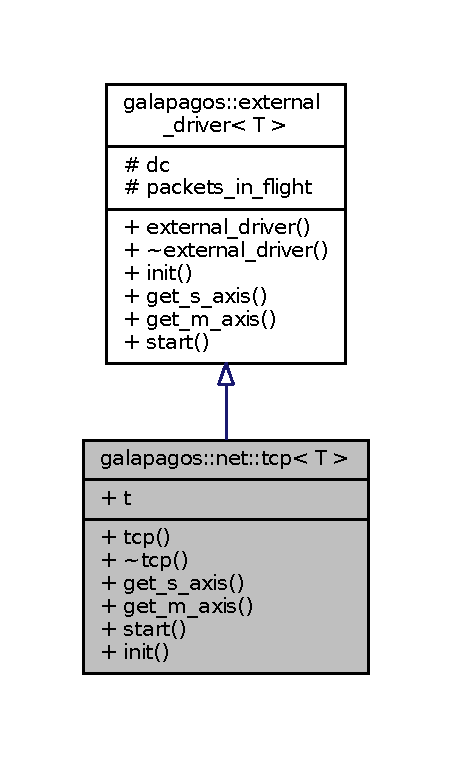
\includegraphics[width=217pt]{classgalapagos_1_1net_1_1tcp__inherit__graph}
\end{center}
\end{figure}


Collaboration diagram for galapagos\+:\+:net\+:\+:tcp$<$ T $>$\+:
\nopagebreak
\begin{figure}[H]
\begin{center}
\leavevmode
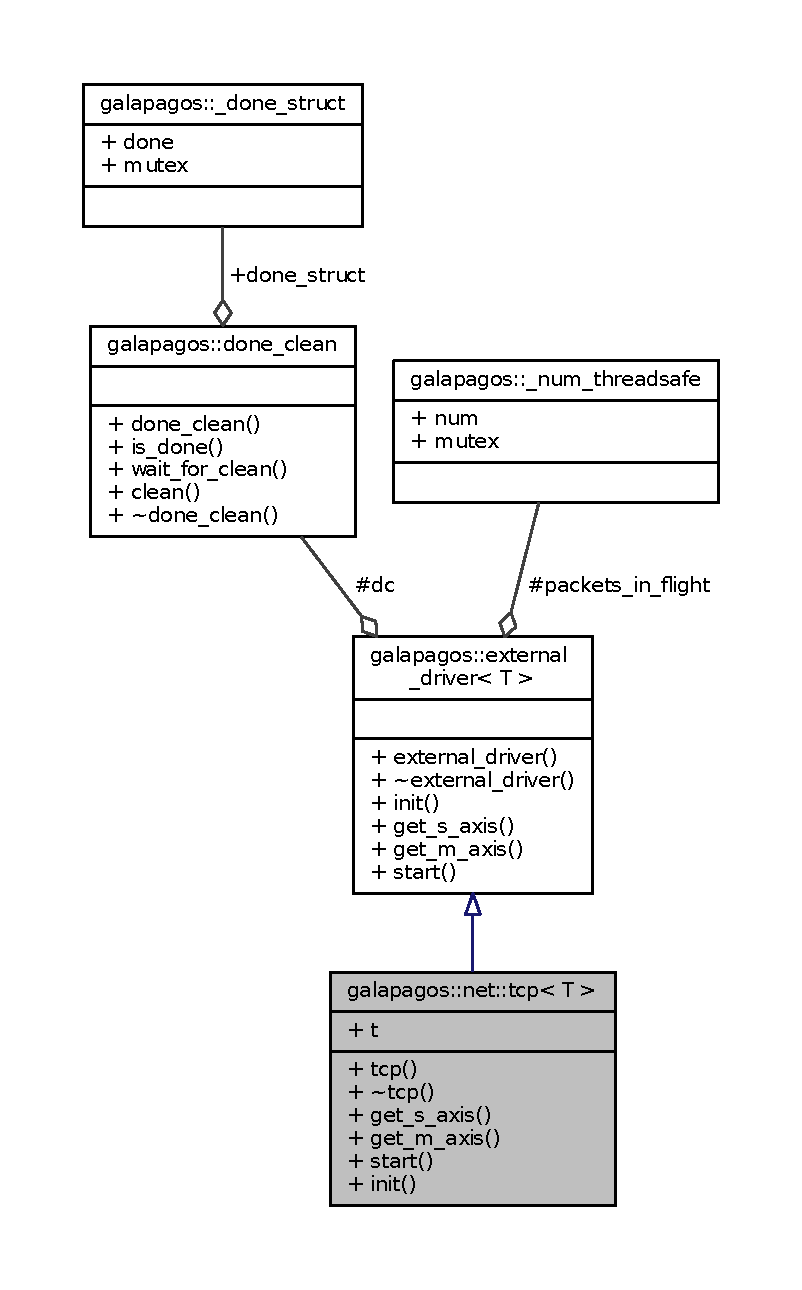
\includegraphics[height=550pt]{classgalapagos_1_1net_1_1tcp__coll__graph}
\end{center}
\end{figure}
\subsection*{Public Member Functions}
\begin{DoxyCompactItemize}
\item 
\hyperlink{classgalapagos_1_1net_1_1tcp_ad739afb4887a1af1388e901b951ede3a}{tcp} (short port, std\+::vector$<$ std\+::string $>$ kern\+\_\+info\+\_\+table, std\+::string my\+\_\+address)
\item 
\hyperlink{classgalapagos_1_1net_1_1tcp_a9908d7aea9bfaf39466706e53cf14437}{$\sim$tcp} ()
\item 
\hyperlink{classgalapagos_1_1interface}{interface}$<$ \hyperlink{test_8cpp_a0658ceffa730c765d449bb3d21871b5f}{T} $>$ $\ast$ \hyperlink{classgalapagos_1_1net_1_1tcp_ac9f3db01e1d6e9bf0bc7527fabf3543a}{get\+\_\+s\+\_\+axis} ()
\item 
\hyperlink{classgalapagos_1_1interface}{interface}$<$ \hyperlink{test_8cpp_a0658ceffa730c765d449bb3d21871b5f}{T} $>$ $\ast$ \hyperlink{classgalapagos_1_1net_1_1tcp_a47f42325519b0dda4c0157f1d897ed75}{get\+\_\+m\+\_\+axis} ()
\item 
void \hyperlink{classgalapagos_1_1net_1_1tcp_ad792d3c67e6e8a79cb18a6d0c4aaecda}{start} ()
\item 
void \hyperlink{classgalapagos_1_1net_1_1tcp_a10e2ca93acd1562162b2a49400be1292}{init} (\hyperlink{classgalapagos_1_1done__clean}{galapagos\+::done\+\_\+clean} $\ast$, int $\ast$\+\_\+packets\+\_\+in\+\_\+flight, std\+::mutex $\ast$\+\_\+mutex\+\_\+packets\+\_\+in\+\_\+flight)
\end{DoxyCompactItemize}
\subsection*{Public Attributes}
\begin{DoxyCompactItemize}
\item 
std\+::unique\+\_\+ptr$<$ std\+::thread $>$ \hyperlink{classgalapagos_1_1net_1_1tcp_a4820fa1fc2a4a396eaf0554042873643}{t}
\end{DoxyCompactItemize}
\subsection*{Additional Inherited Members}


\subsection{Detailed Description}
\subsubsection*{template$<$class T$>$\\*
class galapagos\+::net\+::tcp$<$ T $>$}

Class tcp driver. 

A software implementation of an n to one router, used by network node to arbitrade output of sessions into the node. Routes between input interfaces(s\+\_\+axis) and an output interface(m\+\_\+axis). \begin{DoxyAuthor}{Author}
Naif Tarafdar 
\end{DoxyAuthor}
\begin{DoxyDate}{Date}
April 20, 2019 
\end{DoxyDate}


\subsection{Constructor \& Destructor Documentation}
\index{galapagos\+::net\+::tcp@{galapagos\+::net\+::tcp}!tcp@{tcp}}
\index{tcp@{tcp}!galapagos\+::net\+::tcp@{galapagos\+::net\+::tcp}}
\subsubsection[{\texorpdfstring{tcp(short port, std\+::vector$<$ std\+::string $>$ kern\+\_\+info\+\_\+table, std\+::string my\+\_\+address)}{tcp(short port, std::vector< std::string > kern_info_table, std::string my_address)}}]{\setlength{\rightskip}{0pt plus 5cm}template$<$class T $>$ {\bf galapagos\+::net\+::tcp}$<$ {\bf T} $>$\+::{\bf tcp} (
\begin{DoxyParamCaption}
\item[{short}]{port, }
\item[{std\+::vector$<$ std\+::string $>$}]{kern\+\_\+info\+\_\+table, }
\item[{std\+::string}]{my\+\_\+address}
\end{DoxyParamCaption}
)}\hypertarget{classgalapagos_1_1net_1_1tcp_ad739afb4887a1af1388e901b951ede3a}{}\label{classgalapagos_1_1net_1_1tcp_ad739afb4887a1af1388e901b951ede3a}
\index{galapagos\+::net\+::tcp@{galapagos\+::net\+::tcp}!````~tcp@{$\sim$tcp}}
\index{````~tcp@{$\sim$tcp}!galapagos\+::net\+::tcp@{galapagos\+::net\+::tcp}}
\subsubsection[{\texorpdfstring{$\sim$tcp()}{~tcp()}}]{\setlength{\rightskip}{0pt plus 5cm}template$<$class T $>$ {\bf galapagos\+::net\+::tcp}$<$ {\bf T} $>$\+::$\sim${\bf tcp} (
\begin{DoxyParamCaption}
{}
\end{DoxyParamCaption}
)\hspace{0.3cm}{\ttfamily [inline]}}\hypertarget{classgalapagos_1_1net_1_1tcp_a9908d7aea9bfaf39466706e53cf14437}{}\label{classgalapagos_1_1net_1_1tcp_a9908d7aea9bfaf39466706e53cf14437}


\subsection{Member Function Documentation}
\index{galapagos\+::net\+::tcp@{galapagos\+::net\+::tcp}!get\+\_\+m\+\_\+axis@{get\+\_\+m\+\_\+axis}}
\index{get\+\_\+m\+\_\+axis@{get\+\_\+m\+\_\+axis}!galapagos\+::net\+::tcp@{galapagos\+::net\+::tcp}}
\subsubsection[{\texorpdfstring{get\+\_\+m\+\_\+axis()}{get_m_axis()}}]{\setlength{\rightskip}{0pt plus 5cm}template$<$class T $>$ {\bf galapagos\+::interface}$<$ {\bf T} $>$ $\ast$ {\bf galapagos\+::net\+::tcp}$<$ {\bf T} $>$\+::get\+\_\+m\+\_\+axis (
\begin{DoxyParamCaption}
{}
\end{DoxyParamCaption}
)\hspace{0.3cm}{\ttfamily [virtual]}}\hypertarget{classgalapagos_1_1net_1_1tcp_a47f42325519b0dda4c0157f1d897ed75}{}\label{classgalapagos_1_1net_1_1tcp_a47f42325519b0dda4c0157f1d897ed75}


Implements \hyperlink{classgalapagos_1_1external__driver_abc7938fd7247c7404441473da71a357e}{galapagos\+::external\+\_\+driver$<$ T $>$}.

\index{galapagos\+::net\+::tcp@{galapagos\+::net\+::tcp}!get\+\_\+s\+\_\+axis@{get\+\_\+s\+\_\+axis}}
\index{get\+\_\+s\+\_\+axis@{get\+\_\+s\+\_\+axis}!galapagos\+::net\+::tcp@{galapagos\+::net\+::tcp}}
\subsubsection[{\texorpdfstring{get\+\_\+s\+\_\+axis()}{get_s_axis()}}]{\setlength{\rightskip}{0pt plus 5cm}template$<$class T $>$ {\bf galapagos\+::interface}$<$ {\bf T} $>$ $\ast$ {\bf galapagos\+::net\+::tcp}$<$ {\bf T} $>$\+::get\+\_\+s\+\_\+axis (
\begin{DoxyParamCaption}
{}
\end{DoxyParamCaption}
)\hspace{0.3cm}{\ttfamily [virtual]}}\hypertarget{classgalapagos_1_1net_1_1tcp_ac9f3db01e1d6e9bf0bc7527fabf3543a}{}\label{classgalapagos_1_1net_1_1tcp_ac9f3db01e1d6e9bf0bc7527fabf3543a}


Implements \hyperlink{classgalapagos_1_1external__driver_aded446e9ebbdd03b461f336045aa7cd2}{galapagos\+::external\+\_\+driver$<$ T $>$}.

\index{galapagos\+::net\+::tcp@{galapagos\+::net\+::tcp}!init@{init}}
\index{init@{init}!galapagos\+::net\+::tcp@{galapagos\+::net\+::tcp}}
\subsubsection[{\texorpdfstring{init(galapagos\+::done\+\_\+clean $\ast$, int $\ast$\+\_\+packets\+\_\+in\+\_\+flight, std\+::mutex $\ast$\+\_\+mutex\+\_\+packets\+\_\+in\+\_\+flight)}{init(galapagos::done_clean *, int *_packets_in_flight, std::mutex *_mutex_packets_in_flight)}}]{\setlength{\rightskip}{0pt plus 5cm}template$<$class T $>$ void {\bf galapagos\+::net\+::tcp}$<$ {\bf T} $>$\+::init (
\begin{DoxyParamCaption}
\item[{{\bf galapagos\+::done\+\_\+clean} $\ast$}]{\+\_\+dc, }
\item[{int $\ast$}]{\+\_\+packets\+\_\+in\+\_\+flight, }
\item[{std\+::mutex $\ast$}]{\+\_\+mutex\+\_\+packets\+\_\+in\+\_\+flight}
\end{DoxyParamCaption}
)\hspace{0.3cm}{\ttfamily [virtual]}}\hypertarget{classgalapagos_1_1net_1_1tcp_a10e2ca93acd1562162b2a49400be1292}{}\label{classgalapagos_1_1net_1_1tcp_a10e2ca93acd1562162b2a49400be1292}


Implements \hyperlink{classgalapagos_1_1external__driver_ab8b753325b02ee15efe16158cd3fe119}{galapagos\+::external\+\_\+driver$<$ T $>$}.

\index{galapagos\+::net\+::tcp@{galapagos\+::net\+::tcp}!start@{start}}
\index{start@{start}!galapagos\+::net\+::tcp@{galapagos\+::net\+::tcp}}
\subsubsection[{\texorpdfstring{start()}{start()}}]{\setlength{\rightskip}{0pt plus 5cm}template$<$class T $>$ void {\bf galapagos\+::net\+::tcp}$<$ {\bf T} $>$\+::start (
\begin{DoxyParamCaption}
{}
\end{DoxyParamCaption}
)\hspace{0.3cm}{\ttfamily [virtual]}}\hypertarget{classgalapagos_1_1net_1_1tcp_ad792d3c67e6e8a79cb18a6d0c4aaecda}{}\label{classgalapagos_1_1net_1_1tcp_ad792d3c67e6e8a79cb18a6d0c4aaecda}


Implements \hyperlink{classgalapagos_1_1external__driver_a7eacf72788a4ce6976499e36f1b7b3a6}{galapagos\+::external\+\_\+driver$<$ T $>$}.



\subsection{Member Data Documentation}
\index{galapagos\+::net\+::tcp@{galapagos\+::net\+::tcp}!t@{t}}
\index{t@{t}!galapagos\+::net\+::tcp@{galapagos\+::net\+::tcp}}
\subsubsection[{\texorpdfstring{t}{t}}]{\setlength{\rightskip}{0pt plus 5cm}template$<$class T $>$ std\+::unique\+\_\+ptr$<$std\+::thread$>$ {\bf galapagos\+::net\+::tcp}$<$ {\bf T} $>$\+::t}\hypertarget{classgalapagos_1_1net_1_1tcp_a4820fa1fc2a4a396eaf0554042873643}{}\label{classgalapagos_1_1net_1_1tcp_a4820fa1fc2a4a396eaf0554042873643}


The documentation for this class was generated from the following file\+:\begin{DoxyCompactItemize}
\item 
\hyperlink{galapagos__net__tcp_8hpp}{galapagos\+\_\+net\+\_\+tcp.\+hpp}\end{DoxyCompactItemize}

\hypertarget{classgalapagos_1_1net_1_1tcp__accept__server}{}\section{galapagos\+:\+:net\+:\+:tcp\+\_\+accept\+\_\+server$<$ T $>$ Class Template Reference}
\label{classgalapagos_1_1net_1_1tcp__accept__server}\index{galapagos\+::net\+::tcp\+\_\+accept\+\_\+server$<$ T $>$@{galapagos\+::net\+::tcp\+\_\+accept\+\_\+server$<$ T $>$}}


{\ttfamily \#include $<$galapagos\+\_\+net\+\_\+tcp\+\_\+accept\+\_\+server.\+hpp$>$}



Collaboration diagram for galapagos\+:\+:net\+:\+:tcp\+\_\+accept\+\_\+server$<$ T $>$\+:
\nopagebreak
\begin{figure}[H]
\begin{center}
\leavevmode
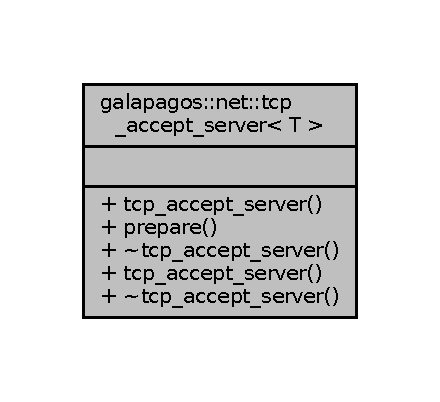
\includegraphics[width=211pt]{classgalapagos_1_1net_1_1tcp__accept__server__coll__graph}
\end{center}
\end{figure}
\subsection*{Public Member Functions}
\begin{DoxyCompactItemize}
\item 
\hyperlink{classgalapagos_1_1net_1_1tcp__accept__server_a44f7191e0eb787b8e5d893ed502415cb}{tcp\+\_\+accept\+\_\+server} (boost\+::asio\+::io\+\_\+context $\ast$io\+\_\+context, std\+::string \hyperlink{test_8cpp_ad6c70ba8571527f1543822ce71b9a109}{my\+\_\+address}, short port, \hyperlink{classgalapagos_1_1net_1_1tcp__session__container}{tcp\+\_\+session\+\_\+container}$<$ \hyperlink{test_8cpp_a0658ceffa730c765d449bb3d21871b5f}{T} $>$ $\ast$\+\_\+sessions)
\item 
void \hyperlink{classgalapagos_1_1net_1_1tcp__accept__server_a7693873e8816380d2157ee1c456988f3}{prepare} (boost\+::asio\+::io\+\_\+context $\ast$io\+\_\+context, std\+::string \hyperlink{test_8cpp_ad6c70ba8571527f1543822ce71b9a109}{my\+\_\+address}, short port, \hyperlink{classgalapagos_1_1net_1_1tcp__session__container}{tcp\+\_\+session\+\_\+container}$<$ \hyperlink{test_8cpp_a0658ceffa730c765d449bb3d21871b5f}{T} $>$ $\ast$\+\_\+sessions)
\item 
\hyperlink{classgalapagos_1_1net_1_1tcp__accept__server_a272d09b62d0cb05324cb2a8f85b8ae64}{$\sim$tcp\+\_\+accept\+\_\+server} ()
\item 
\hyperlink{classgalapagos_1_1net_1_1tcp__accept__server_abf68f05d1d381293ca44f06afa10c0b8}{tcp\+\_\+accept\+\_\+server} (boost\+::asio\+::io\+\_\+context $\ast$io\+\_\+context, std\+::string \hyperlink{test_8cpp_ad6c70ba8571527f1543822ce71b9a109}{my\+\_\+address}, short port, \hyperlink{classgalapagos_1_1net_1_1tcp__session__container}{tcp\+\_\+session\+\_\+container}$<$ \hyperlink{test_8cpp_a0658ceffa730c765d449bb3d21871b5f}{T} $>$ $\ast$\+\_\+sessions)
\item 
\hyperlink{classgalapagos_1_1net_1_1tcp__accept__server_a272d09b62d0cb05324cb2a8f85b8ae64}{$\sim$tcp\+\_\+accept\+\_\+server} ()
\end{DoxyCompactItemize}


\subsection{Constructor \& Destructor Documentation}
\index{galapagos\+::net\+::tcp\+\_\+accept\+\_\+server@{galapagos\+::net\+::tcp\+\_\+accept\+\_\+server}!tcp\+\_\+accept\+\_\+server@{tcp\+\_\+accept\+\_\+server}}
\index{tcp\+\_\+accept\+\_\+server@{tcp\+\_\+accept\+\_\+server}!galapagos\+::net\+::tcp\+\_\+accept\+\_\+server@{galapagos\+::net\+::tcp\+\_\+accept\+\_\+server}}
\subsubsection[{\texorpdfstring{tcp\+\_\+accept\+\_\+server(boost\+::asio\+::io\+\_\+context $\ast$io\+\_\+context, std\+::string my\+\_\+address, short port, tcp\+\_\+session\+\_\+container$<$ T $>$ $\ast$\+\_\+sessions)}{tcp_accept_server(boost::asio::io_context *io_context, std::string my_address, short port, tcp_session_container< T > *_sessions)}}]{\setlength{\rightskip}{0pt plus 5cm}template$<$class T $>$ tcp\+\_\+accept\+\_\+server\+::tcp\+\_\+accept\+\_\+server (
\begin{DoxyParamCaption}
\item[{boost\+::asio\+::io\+\_\+context $\ast$}]{io\+\_\+context, }
\item[{std\+::string}]{my\+\_\+address, }
\item[{short}]{port, }
\item[{{\bf tcp\+\_\+session\+\_\+container}$<$ {\bf T} $>$ $\ast$}]{\+\_\+sessions}
\end{DoxyParamCaption}
)}\hypertarget{classgalapagos_1_1net_1_1tcp__accept__server_a44f7191e0eb787b8e5d893ed502415cb}{}\label{classgalapagos_1_1net_1_1tcp__accept__server_a44f7191e0eb787b8e5d893ed502415cb}
\index{galapagos\+::net\+::tcp\+\_\+accept\+\_\+server@{galapagos\+::net\+::tcp\+\_\+accept\+\_\+server}!````~tcp\+\_\+accept\+\_\+server@{$\sim$tcp\+\_\+accept\+\_\+server}}
\index{````~tcp\+\_\+accept\+\_\+server@{$\sim$tcp\+\_\+accept\+\_\+server}!galapagos\+::net\+::tcp\+\_\+accept\+\_\+server@{galapagos\+::net\+::tcp\+\_\+accept\+\_\+server}}
\subsubsection[{\texorpdfstring{$\sim$tcp\+\_\+accept\+\_\+server()}{~tcp_accept_server()}}]{\setlength{\rightskip}{0pt plus 5cm}template$<$class T $>$ {\bf galapagos\+::net\+::tcp\+\_\+accept\+\_\+server}$<$ {\bf T} $>$\+::$\sim${\bf tcp\+\_\+accept\+\_\+server} (
\begin{DoxyParamCaption}
{}
\end{DoxyParamCaption}
)\hspace{0.3cm}{\ttfamily [inline]}}\hypertarget{classgalapagos_1_1net_1_1tcp__accept__server_a272d09b62d0cb05324cb2a8f85b8ae64}{}\label{classgalapagos_1_1net_1_1tcp__accept__server_a272d09b62d0cb05324cb2a8f85b8ae64}
\index{galapagos\+::net\+::tcp\+\_\+accept\+\_\+server@{galapagos\+::net\+::tcp\+\_\+accept\+\_\+server}!tcp\+\_\+accept\+\_\+server@{tcp\+\_\+accept\+\_\+server}}
\index{tcp\+\_\+accept\+\_\+server@{tcp\+\_\+accept\+\_\+server}!galapagos\+::net\+::tcp\+\_\+accept\+\_\+server@{galapagos\+::net\+::tcp\+\_\+accept\+\_\+server}}
\subsubsection[{\texorpdfstring{tcp\+\_\+accept\+\_\+server(boost\+::asio\+::io\+\_\+context $\ast$io\+\_\+context, std\+::string my\+\_\+address, short port, tcp\+\_\+session\+\_\+container$<$ T $>$ $\ast$\+\_\+sessions)}{tcp_accept_server(boost::asio::io_context *io_context, std::string my_address, short port, tcp_session_container< T > *_sessions)}}]{\setlength{\rightskip}{0pt plus 5cm}template$<$class T $>$ {\bf galapagos\+::net\+::tcp\+\_\+accept\+\_\+server}$<$ {\bf T} $>$\+::{\bf tcp\+\_\+accept\+\_\+server} (
\begin{DoxyParamCaption}
\item[{boost\+::asio\+::io\+\_\+context $\ast$}]{io\+\_\+context, }
\item[{std\+::string}]{my\+\_\+address, }
\item[{short}]{port, }
\item[{{\bf tcp\+\_\+session\+\_\+container}$<$ {\bf T} $>$ $\ast$}]{\+\_\+sessions}
\end{DoxyParamCaption}
)}\hypertarget{classgalapagos_1_1net_1_1tcp__accept__server_abf68f05d1d381293ca44f06afa10c0b8}{}\label{classgalapagos_1_1net_1_1tcp__accept__server_abf68f05d1d381293ca44f06afa10c0b8}
\index{galapagos\+::net\+::tcp\+\_\+accept\+\_\+server@{galapagos\+::net\+::tcp\+\_\+accept\+\_\+server}!````~tcp\+\_\+accept\+\_\+server@{$\sim$tcp\+\_\+accept\+\_\+server}}
\index{````~tcp\+\_\+accept\+\_\+server@{$\sim$tcp\+\_\+accept\+\_\+server}!galapagos\+::net\+::tcp\+\_\+accept\+\_\+server@{galapagos\+::net\+::tcp\+\_\+accept\+\_\+server}}
\subsubsection[{\texorpdfstring{$\sim$tcp\+\_\+accept\+\_\+server()}{~tcp_accept_server()}}]{\setlength{\rightskip}{0pt plus 5cm}template$<$class T $>$ {\bf galapagos\+::net\+::tcp\+\_\+accept\+\_\+server}$<$ {\bf T} $>$\+::$\sim${\bf tcp\+\_\+accept\+\_\+server} (
\begin{DoxyParamCaption}
{}
\end{DoxyParamCaption}
)\hspace{0.3cm}{\ttfamily [inline]}}\hypertarget{classgalapagos_1_1net_1_1tcp__accept__server_a272d09b62d0cb05324cb2a8f85b8ae64}{}\label{classgalapagos_1_1net_1_1tcp__accept__server_a272d09b62d0cb05324cb2a8f85b8ae64}


\subsection{Member Function Documentation}
\index{galapagos\+::net\+::tcp\+\_\+accept\+\_\+server@{galapagos\+::net\+::tcp\+\_\+accept\+\_\+server}!prepare@{prepare}}
\index{prepare@{prepare}!galapagos\+::net\+::tcp\+\_\+accept\+\_\+server@{galapagos\+::net\+::tcp\+\_\+accept\+\_\+server}}
\subsubsection[{\texorpdfstring{prepare(boost\+::asio\+::io\+\_\+context $\ast$io\+\_\+context, std\+::string my\+\_\+address, short port, tcp\+\_\+session\+\_\+container$<$ T $>$ $\ast$\+\_\+sessions)}{prepare(boost::asio::io_context *io_context, std::string my_address, short port, tcp_session_container< T > *_sessions)}}]{\setlength{\rightskip}{0pt plus 5cm}template$<$class T $>$ void tcp\+\_\+accept\+\_\+server\+::prepare (
\begin{DoxyParamCaption}
\item[{boost\+::asio\+::io\+\_\+context $\ast$}]{io\+\_\+context, }
\item[{std\+::string}]{my\+\_\+address, }
\item[{short}]{port, }
\item[{{\bf tcp\+\_\+session\+\_\+container}$<$ {\bf T} $>$ $\ast$}]{\+\_\+sessions}
\end{DoxyParamCaption}
)}\hypertarget{classgalapagos_1_1net_1_1tcp__accept__server_a7693873e8816380d2157ee1c456988f3}{}\label{classgalapagos_1_1net_1_1tcp__accept__server_a7693873e8816380d2157ee1c456988f3}


The documentation for this class was generated from the following files\+:\begin{DoxyCompactItemize}
\item 
\hyperlink{galapagos__net__tcp__accept__server_8hpp}{galapagos\+\_\+net\+\_\+tcp\+\_\+accept\+\_\+server.\+hpp}\item 
\hyperlink{galapagos__net__udp__accept__server_8hpp}{galapagos\+\_\+net\+\_\+udp\+\_\+accept\+\_\+server.\+hpp}\end{DoxyCompactItemize}

\hypertarget{classgalapagos_1_1net_1_1tcp__server__send}{}\section{galapagos\+:\+:net\+:\+:tcp\+\_\+server\+\_\+send$<$ T $>$ Class Template Reference}
\label{classgalapagos_1_1net_1_1tcp__server__send}\index{galapagos\+::net\+::tcp\+\_\+server\+\_\+send$<$ T $>$@{galapagos\+::net\+::tcp\+\_\+server\+\_\+send$<$ T $>$}}


Class for the \hyperlink{classgalapagos_1_1net_1_1tcp__server__send}{tcp\+\_\+server\+\_\+send}, responsible for sending packets to sessions.  




{\ttfamily \#include $<$galapagos\+\_\+net\+\_\+tcp\+\_\+server\+\_\+send.\+hpp$>$}



Collaboration diagram for galapagos\+:\+:net\+:\+:tcp\+\_\+server\+\_\+send$<$ T $>$\+:
\nopagebreak
\begin{figure}[H]
\begin{center}
\leavevmode
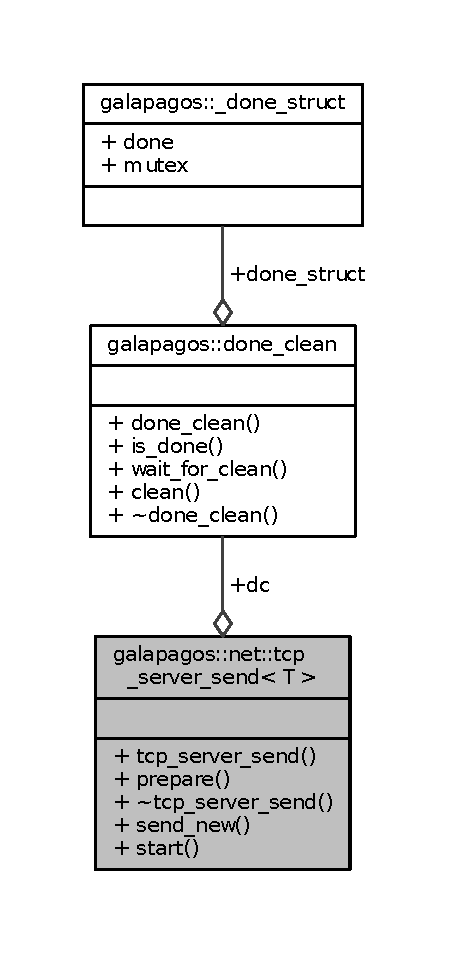
\includegraphics[width=216pt]{classgalapagos_1_1net_1_1tcp__server__send__coll__graph}
\end{center}
\end{figure}
\subsection*{Public Member Functions}
\begin{DoxyCompactItemize}
\item 
\hyperlink{classgalapagos_1_1net_1_1tcp__server__send_a3857d5f1fd45bb269867d5e0f99e5248}{tcp\+\_\+server\+\_\+send} (short \+\_\+port, boost\+::asio\+::io\+\_\+context $\ast$\+\_\+io\+\_\+context, \hyperlink{classgalapagos_1_1net_1_1tcp__session__container}{tcp\+\_\+session\+\_\+container}$<$ \hyperlink{test_8cpp_a0658ceffa730c765d449bb3d21871b5f}{T} $>$ $\ast$\+\_\+sessions, \hyperlink{classgalapagos_1_1done__clean}{done\+\_\+clean} $\ast$\+\_\+dc, \hyperlink{classgalapagos_1_1interface}{interface}$<$ \hyperlink{test_8cpp_a0658ceffa730c765d449bb3d21871b5f}{T} $>$ $\ast$\+\_\+s\+\_\+axis)
\item 
void \hyperlink{classgalapagos_1_1net_1_1tcp__server__send_a14d064e2ad5e0185c0bada4edfff1426}{prepare} (short \+\_\+port, boost\+::asio\+::io\+\_\+context $\ast$\+\_\+io\+\_\+context, \hyperlink{classgalapagos_1_1net_1_1tcp__session__container}{tcp\+\_\+session\+\_\+container}$<$ \hyperlink{test_8cpp_a0658ceffa730c765d449bb3d21871b5f}{T} $>$ $\ast$\+\_\+sessions, \hyperlink{classgalapagos_1_1done__clean}{done\+\_\+clean} $\ast$\+\_\+dc, \hyperlink{classgalapagos_1_1interface}{interface}$<$ \hyperlink{test_8cpp_a0658ceffa730c765d449bb3d21871b5f}{T} $>$ $\ast$\+\_\+s\+\_\+axis)
\item 
\hyperlink{classgalapagos_1_1net_1_1tcp__server__send_ab18eee975ce0c0d4cc93a293c1ab710e}{$\sim$tcp\+\_\+server\+\_\+send} ()
\item 
void \hyperlink{classgalapagos_1_1net_1_1tcp__server__send_a30cd97b5cb1b51846065a75121fb2656}{send\+\_\+new} (std\+::string ip\+\_\+addr)
\item 
void \hyperlink{classgalapagos_1_1net_1_1tcp__server__send_ade3b0a11a7025ce84b93bca633d9f793}{start} ()
\end{DoxyCompactItemize}
\subsection*{Public Attributes}
\begin{DoxyCompactItemize}
\item 
\hyperlink{classgalapagos_1_1done__clean}{done\+\_\+clean} $\ast$ \hyperlink{classgalapagos_1_1net_1_1tcp__server__send_ae17e0980a0d49b50cb59a98a6774241d}{dc}
\end{DoxyCompactItemize}


\subsection{Detailed Description}
\subsubsection*{template$<$class T$>$\\*
class galapagos\+::net\+::tcp\+\_\+server\+\_\+send$<$ T $>$}

Class for the \hyperlink{classgalapagos_1_1net_1_1tcp__server__send}{tcp\+\_\+server\+\_\+send}, responsible for sending packets to sessions. 

Runs as daemon in background, with an s\+\_\+axis interface. If receives something on s\+\_\+axis, then checks to see if a session exists, if it does then writes into s\+\_\+axis of session, else creates a new session and then writes into s\+\_\+axis of that session. \begin{DoxyAuthor}{Author}
Naif Tarafdar 
\end{DoxyAuthor}
\begin{DoxyDate}{Date}
April 20, 2019 
\end{DoxyDate}


\subsection{Constructor \& Destructor Documentation}
\index{galapagos\+::net\+::tcp\+\_\+server\+\_\+send@{galapagos\+::net\+::tcp\+\_\+server\+\_\+send}!tcp\+\_\+server\+\_\+send@{tcp\+\_\+server\+\_\+send}}
\index{tcp\+\_\+server\+\_\+send@{tcp\+\_\+server\+\_\+send}!galapagos\+::net\+::tcp\+\_\+server\+\_\+send@{galapagos\+::net\+::tcp\+\_\+server\+\_\+send}}
\subsubsection[{\texorpdfstring{tcp\+\_\+server\+\_\+send(short \+\_\+port, boost\+::asio\+::io\+\_\+context $\ast$\+\_\+io\+\_\+context, tcp\+\_\+session\+\_\+container$<$ T $>$ $\ast$\+\_\+sessions, done\+\_\+clean $\ast$\+\_\+dc, interface$<$ T $>$ $\ast$\+\_\+s\+\_\+axis)}{tcp_server_send(short _port, boost::asio::io_context *_io_context, tcp_session_container< T > *_sessions, done_clean *_dc, interface< T > *_s_axis)}}]{\setlength{\rightskip}{0pt plus 5cm}template$<$class T $>$ tcp\+\_\+server\+\_\+send\+::tcp\+\_\+server\+\_\+send (
\begin{DoxyParamCaption}
\item[{short}]{\+\_\+port, }
\item[{boost\+::asio\+::io\+\_\+context $\ast$}]{\+\_\+io\+\_\+context, }
\item[{{\bf tcp\+\_\+session\+\_\+container}$<$ {\bf T} $>$ $\ast$}]{\+\_\+sessions, }
\item[{{\bf done\+\_\+clean} $\ast$}]{\+\_\+dc, }
\item[{{\bf interface}$<$ {\bf T} $>$ $\ast$}]{\+\_\+s\+\_\+axis}
\end{DoxyParamCaption}
)}\hypertarget{classgalapagos_1_1net_1_1tcp__server__send_a3857d5f1fd45bb269867d5e0f99e5248}{}\label{classgalapagos_1_1net_1_1tcp__server__send_a3857d5f1fd45bb269867d5e0f99e5248}
\index{galapagos\+::net\+::tcp\+\_\+server\+\_\+send@{galapagos\+::net\+::tcp\+\_\+server\+\_\+send}!````~tcp\+\_\+server\+\_\+send@{$\sim$tcp\+\_\+server\+\_\+send}}
\index{````~tcp\+\_\+server\+\_\+send@{$\sim$tcp\+\_\+server\+\_\+send}!galapagos\+::net\+::tcp\+\_\+server\+\_\+send@{galapagos\+::net\+::tcp\+\_\+server\+\_\+send}}
\subsubsection[{\texorpdfstring{$\sim$tcp\+\_\+server\+\_\+send()}{~tcp_server_send()}}]{\setlength{\rightskip}{0pt plus 5cm}template$<$class T $>$ {\bf galapagos\+::net\+::tcp\+\_\+server\+\_\+send}$<$ {\bf T} $>$\+::$\sim${\bf tcp\+\_\+server\+\_\+send} (
\begin{DoxyParamCaption}
{}
\end{DoxyParamCaption}
)\hspace{0.3cm}{\ttfamily [inline]}}\hypertarget{classgalapagos_1_1net_1_1tcp__server__send_ab18eee975ce0c0d4cc93a293c1ab710e}{}\label{classgalapagos_1_1net_1_1tcp__server__send_ab18eee975ce0c0d4cc93a293c1ab710e}


\subsection{Member Function Documentation}
\index{galapagos\+::net\+::tcp\+\_\+server\+\_\+send@{galapagos\+::net\+::tcp\+\_\+server\+\_\+send}!prepare@{prepare}}
\index{prepare@{prepare}!galapagos\+::net\+::tcp\+\_\+server\+\_\+send@{galapagos\+::net\+::tcp\+\_\+server\+\_\+send}}
\subsubsection[{\texorpdfstring{prepare(short \+\_\+port, boost\+::asio\+::io\+\_\+context $\ast$\+\_\+io\+\_\+context, tcp\+\_\+session\+\_\+container$<$ T $>$ $\ast$\+\_\+sessions, done\+\_\+clean $\ast$\+\_\+dc, interface$<$ T $>$ $\ast$\+\_\+s\+\_\+axis)}{prepare(short _port, boost::asio::io_context *_io_context, tcp_session_container< T > *_sessions, done_clean *_dc, interface< T > *_s_axis)}}]{\setlength{\rightskip}{0pt plus 5cm}template$<$class T $>$ void tcp\+\_\+server\+\_\+send\+::prepare (
\begin{DoxyParamCaption}
\item[{short}]{\+\_\+port, }
\item[{boost\+::asio\+::io\+\_\+context $\ast$}]{\+\_\+io\+\_\+context, }
\item[{{\bf tcp\+\_\+session\+\_\+container}$<$ {\bf T} $>$ $\ast$}]{\+\_\+sessions, }
\item[{{\bf done\+\_\+clean} $\ast$}]{\+\_\+dc, }
\item[{{\bf interface}$<$ {\bf T} $>$ $\ast$}]{\+\_\+s\+\_\+axis}
\end{DoxyParamCaption}
)}\hypertarget{classgalapagos_1_1net_1_1tcp__server__send_a14d064e2ad5e0185c0bada4edfff1426}{}\label{classgalapagos_1_1net_1_1tcp__server__send_a14d064e2ad5e0185c0bada4edfff1426}
\index{galapagos\+::net\+::tcp\+\_\+server\+\_\+send@{galapagos\+::net\+::tcp\+\_\+server\+\_\+send}!send\+\_\+new@{send\+\_\+new}}
\index{send\+\_\+new@{send\+\_\+new}!galapagos\+::net\+::tcp\+\_\+server\+\_\+send@{galapagos\+::net\+::tcp\+\_\+server\+\_\+send}}
\subsubsection[{\texorpdfstring{send\+\_\+new(std\+::string ip\+\_\+addr)}{send_new(std::string ip_addr)}}]{\setlength{\rightskip}{0pt plus 5cm}template$<$class T $>$ void tcp\+\_\+server\+\_\+send\+::send\+\_\+new (
\begin{DoxyParamCaption}
\item[{std\+::string}]{ip\+\_\+addr}
\end{DoxyParamCaption}
)}\hypertarget{classgalapagos_1_1net_1_1tcp__server__send_a30cd97b5cb1b51846065a75121fb2656}{}\label{classgalapagos_1_1net_1_1tcp__server__send_a30cd97b5cb1b51846065a75121fb2656}
Creates a T\+CP session before sending data to session 
\begin{DoxyTemplParams}{Template Parameters}
{\em T} & the type of data used within each galapagos packet (default ap\+\_\+uint$<$64$>$) \\
\hline
\end{DoxyTemplParams}

\begin{DoxyParams}[1]{Parameters}
\mbox{\tt in}  & {\em ip\+\_\+addr} & address to create session \\
\hline
\end{DoxyParams}
\index{galapagos\+::net\+::tcp\+\_\+server\+\_\+send@{galapagos\+::net\+::tcp\+\_\+server\+\_\+send}!start@{start}}
\index{start@{start}!galapagos\+::net\+::tcp\+\_\+server\+\_\+send@{galapagos\+::net\+::tcp\+\_\+server\+\_\+send}}
\subsubsection[{\texorpdfstring{start()}{start()}}]{\setlength{\rightskip}{0pt plus 5cm}template$<$class T $>$ void tcp\+\_\+server\+\_\+send\+::start (
\begin{DoxyParamCaption}
{}
\end{DoxyParamCaption}
)}\hypertarget{classgalapagos_1_1net_1_1tcp__server__send_ade3b0a11a7025ce84b93bca633d9f793}{}\label{classgalapagos_1_1net_1_1tcp__server__send_ade3b0a11a7025ce84b93bca633d9f793}


\subsection{Member Data Documentation}
\index{galapagos\+::net\+::tcp\+\_\+server\+\_\+send@{galapagos\+::net\+::tcp\+\_\+server\+\_\+send}!dc@{dc}}
\index{dc@{dc}!galapagos\+::net\+::tcp\+\_\+server\+\_\+send@{galapagos\+::net\+::tcp\+\_\+server\+\_\+send}}
\subsubsection[{\texorpdfstring{dc}{dc}}]{\setlength{\rightskip}{0pt plus 5cm}template$<$class T $>$ {\bf done\+\_\+clean}$\ast$ {\bf galapagos\+::net\+::tcp\+\_\+server\+\_\+send}$<$ {\bf T} $>$\+::dc}\hypertarget{classgalapagos_1_1net_1_1tcp__server__send_ae17e0980a0d49b50cb59a98a6774241d}{}\label{classgalapagos_1_1net_1_1tcp__server__send_ae17e0980a0d49b50cb59a98a6774241d}


The documentation for this class was generated from the following file\+:\begin{DoxyCompactItemize}
\item 
\hyperlink{galapagos__net__tcp__server__send_8hpp}{galapagos\+\_\+net\+\_\+tcp\+\_\+server\+\_\+send.\+hpp}\end{DoxyCompactItemize}

\hypertarget{classgalapagos_1_1net_1_1tcp__session}{}\section{galapagos\+:\+:net\+:\+:tcp\+\_\+session$<$ T $>$ Class Template Reference}
\label{classgalapagos_1_1net_1_1tcp__session}\index{galapagos\+::net\+::tcp\+\_\+session$<$ T $>$@{galapagos\+::net\+::tcp\+\_\+session$<$ T $>$}}


Class for the \hyperlink{classgalapagos_1_1net_1_1tcp__session}{tcp\+\_\+session}.  




{\ttfamily \#include $<$galapagos\+\_\+net\+\_\+tcp\+\_\+session.\+hpp$>$}



Collaboration diagram for galapagos\+:\+:net\+:\+:tcp\+\_\+session$<$ T $>$\+:
\nopagebreak
\begin{figure}[H]
\begin{center}
\leavevmode
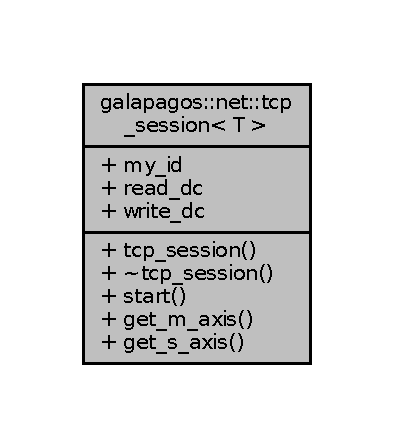
\includegraphics[width=189pt]{classgalapagos_1_1net_1_1tcp__session__coll__graph}
\end{center}
\end{figure}
\subsection*{Public Member Functions}
\begin{DoxyCompactItemize}
\item 
\hyperlink{classgalapagos_1_1net_1_1tcp__session_ab893344dbd9d66ca8d21f40a76ec3ce0}{tcp\+\_\+session} (boost\+::asio\+::ip\+::tcp\+::socket \+\_\+socket, boost\+::asio\+::io\+\_\+context $\ast$\+\_\+io\+\_\+context, std\+::mutex $\ast$\+\_\+mutex\+\_\+packets\+\_\+in\+\_\+flight, int $\ast$\+\_\+packets\+\_\+in\+\_\+flight, short \+\_\+id, \hyperlink{classgalapagos_1_1done__clean}{done\+\_\+clean} $\ast$\+\_\+dc)
\item 
\hyperlink{classgalapagos_1_1net_1_1tcp__session_aa78485373ac174037d97bcb07e89e7d1}{$\sim$tcp\+\_\+session} ()
\item 
void \hyperlink{classgalapagos_1_1net_1_1tcp__session_a05dba3e74c5eb60feae0d480ba680595}{start} ()
\item 
\hyperlink{classgalapagos_1_1interface}{interface}$<$ \hyperlink{test_8cpp_a0658ceffa730c765d449bb3d21871b5f}{T} $>$ $\ast$ \hyperlink{classgalapagos_1_1net_1_1tcp__session_ab92743d088c4d3da7da60ce9dd083d53}{get\+\_\+m\+\_\+axis} ()
\item 
\hyperlink{classgalapagos_1_1interface}{interface}$<$ \hyperlink{test_8cpp_a0658ceffa730c765d449bb3d21871b5f}{T} $>$ $\ast$ \hyperlink{classgalapagos_1_1net_1_1tcp__session_abd5d37151d61838bd1a869d65cb4f7f0}{get\+\_\+s\+\_\+axis} ()
\end{DoxyCompactItemize}
\subsection*{Public Attributes}
\begin{DoxyCompactItemize}
\item 
short \hyperlink{classgalapagos_1_1net_1_1tcp__session_aefce375d01a745fe43f8a95f9287e42c}{my\+\_\+id}
\item 
std\+::unique\+\_\+ptr$<$ \hyperlink{classgalapagos_1_1done__clean}{galapagos\+::done\+\_\+clean} $>$ \hyperlink{classgalapagos_1_1net_1_1tcp__session_a532c328580ac4fcd0fc6fd5eea889b9d}{read\+\_\+dc}
\item 
std\+::unique\+\_\+ptr$<$ \hyperlink{classgalapagos_1_1done__clean}{galapagos\+::done\+\_\+clean} $>$ \hyperlink{classgalapagos_1_1net_1_1tcp__session_ac368eff45244f67202dab352444f0369}{write\+\_\+dc}
\end{DoxyCompactItemize}


\subsection{Detailed Description}
\subsubsection*{template$<$class T$>$\\*
class galapagos\+::net\+::tcp\+\_\+session$<$ T $>$}

Class for the \hyperlink{classgalapagos_1_1net_1_1tcp__session}{tcp\+\_\+session}. 

T\+CP session, individual session per each kernel not within this node. Contains an interface in, and interface out \begin{DoxyAuthor}{Author}
Naif Tarafdar 
\end{DoxyAuthor}
\begin{DoxyDate}{Date}
April 20, 2019 
\end{DoxyDate}


\subsection{Constructor \& Destructor Documentation}
\index{galapagos\+::net\+::tcp\+\_\+session@{galapagos\+::net\+::tcp\+\_\+session}!tcp\+\_\+session@{tcp\+\_\+session}}
\index{tcp\+\_\+session@{tcp\+\_\+session}!galapagos\+::net\+::tcp\+\_\+session@{galapagos\+::net\+::tcp\+\_\+session}}
\subsubsection[{\texorpdfstring{tcp\+\_\+session(boost\+::asio\+::ip\+::tcp\+::socket \+\_\+socket, boost\+::asio\+::io\+\_\+context $\ast$\+\_\+io\+\_\+context, std\+::mutex $\ast$\+\_\+mutex\+\_\+packets\+\_\+in\+\_\+flight, int $\ast$\+\_\+packets\+\_\+in\+\_\+flight, short \+\_\+id, done\+\_\+clean $\ast$\+\_\+dc)}{tcp_session(boost::asio::ip::tcp::socket _socket, boost::asio::io_context *_io_context, std::mutex *_mutex_packets_in_flight, int *_packets_in_flight, short _id, done_clean *_dc)}}]{\setlength{\rightskip}{0pt plus 5cm}template$<$class T $>$ tcp\+\_\+session\+::tcp\+\_\+session (
\begin{DoxyParamCaption}
\item[{boost\+::asio\+::ip\+::tcp\+::socket}]{\+\_\+socket, }
\item[{boost\+::asio\+::io\+\_\+context $\ast$}]{\+\_\+io\+\_\+context, }
\item[{std\+::mutex $\ast$}]{\+\_\+mutex\+\_\+packets\+\_\+in\+\_\+flight, }
\item[{int $\ast$}]{\+\_\+packets\+\_\+in\+\_\+flight, }
\item[{short}]{\+\_\+id, }
\item[{{\bf galapagos\+::done\+\_\+clean} $\ast$}]{\+\_\+dc}
\end{DoxyParamCaption}
)}\hypertarget{classgalapagos_1_1net_1_1tcp__session_ab893344dbd9d66ca8d21f40a76ec3ce0}{}\label{classgalapagos_1_1net_1_1tcp__session_ab893344dbd9d66ca8d21f40a76ec3ce0}
\index{galapagos\+::net\+::tcp\+\_\+session@{galapagos\+::net\+::tcp\+\_\+session}!````~tcp\+\_\+session@{$\sim$tcp\+\_\+session}}
\index{````~tcp\+\_\+session@{$\sim$tcp\+\_\+session}!galapagos\+::net\+::tcp\+\_\+session@{galapagos\+::net\+::tcp\+\_\+session}}
\subsubsection[{\texorpdfstring{$\sim$tcp\+\_\+session()}{~tcp_session()}}]{\setlength{\rightskip}{0pt plus 5cm}template$<$class T $>$ {\bf galapagos\+::net\+::tcp\+\_\+session}$<$ {\bf T} $>$\+::$\sim${\bf tcp\+\_\+session} (
\begin{DoxyParamCaption}
{}
\end{DoxyParamCaption}
)\hspace{0.3cm}{\ttfamily [inline]}}\hypertarget{classgalapagos_1_1net_1_1tcp__session_aa78485373ac174037d97bcb07e89e7d1}{}\label{classgalapagos_1_1net_1_1tcp__session_aa78485373ac174037d97bcb07e89e7d1}


\subsection{Member Function Documentation}
\index{galapagos\+::net\+::tcp\+\_\+session@{galapagos\+::net\+::tcp\+\_\+session}!get\+\_\+m\+\_\+axis@{get\+\_\+m\+\_\+axis}}
\index{get\+\_\+m\+\_\+axis@{get\+\_\+m\+\_\+axis}!galapagos\+::net\+::tcp\+\_\+session@{galapagos\+::net\+::tcp\+\_\+session}}
\subsubsection[{\texorpdfstring{get\+\_\+m\+\_\+axis()}{get_m_axis()}}]{\setlength{\rightskip}{0pt plus 5cm}template$<$class T $>$ {\bf galapagos\+::interface}$<$ {\bf T} $>$ $\ast$ tcp\+\_\+session\+::get\+\_\+m\+\_\+axis (
\begin{DoxyParamCaption}
{}
\end{DoxyParamCaption}
)}\hypertarget{classgalapagos_1_1net_1_1tcp__session_ab92743d088c4d3da7da60ce9dd083d53}{}\label{classgalapagos_1_1net_1_1tcp__session_ab92743d088c4d3da7da60ce9dd083d53}
\index{galapagos\+::net\+::tcp\+\_\+session@{galapagos\+::net\+::tcp\+\_\+session}!get\+\_\+s\+\_\+axis@{get\+\_\+s\+\_\+axis}}
\index{get\+\_\+s\+\_\+axis@{get\+\_\+s\+\_\+axis}!galapagos\+::net\+::tcp\+\_\+session@{galapagos\+::net\+::tcp\+\_\+session}}
\subsubsection[{\texorpdfstring{get\+\_\+s\+\_\+axis()}{get_s_axis()}}]{\setlength{\rightskip}{0pt plus 5cm}template$<$class T $>$ {\bf galapagos\+::interface}$<$ {\bf T} $>$ $\ast$ tcp\+\_\+session\+::get\+\_\+s\+\_\+axis (
\begin{DoxyParamCaption}
{}
\end{DoxyParamCaption}
)}\hypertarget{classgalapagos_1_1net_1_1tcp__session_abd5d37151d61838bd1a869d65cb4f7f0}{}\label{classgalapagos_1_1net_1_1tcp__session_abd5d37151d61838bd1a869d65cb4f7f0}
\index{galapagos\+::net\+::tcp\+\_\+session@{galapagos\+::net\+::tcp\+\_\+session}!start@{start}}
\index{start@{start}!galapagos\+::net\+::tcp\+\_\+session@{galapagos\+::net\+::tcp\+\_\+session}}
\subsubsection[{\texorpdfstring{start()}{start()}}]{\setlength{\rightskip}{0pt plus 5cm}template$<$class T $>$ void tcp\+\_\+session\+::start (
\begin{DoxyParamCaption}
{}
\end{DoxyParamCaption}
)}\hypertarget{classgalapagos_1_1net_1_1tcp__session_a05dba3e74c5eb60feae0d480ba680595}{}\label{classgalapagos_1_1net_1_1tcp__session_a05dba3e74c5eb60feae0d480ba680595}
Starts the tcp session read and write functions 
\begin{DoxyTemplParams}{Template Parameters}
{\em T} & the type of data used within each galapagos packet (default ap\+\_\+uint$<$64$>$) \\
\hline
\end{DoxyTemplParams}


\subsection{Member Data Documentation}
\index{galapagos\+::net\+::tcp\+\_\+session@{galapagos\+::net\+::tcp\+\_\+session}!my\+\_\+id@{my\+\_\+id}}
\index{my\+\_\+id@{my\+\_\+id}!galapagos\+::net\+::tcp\+\_\+session@{galapagos\+::net\+::tcp\+\_\+session}}
\subsubsection[{\texorpdfstring{my\+\_\+id}{my_id}}]{\setlength{\rightskip}{0pt plus 5cm}template$<$class T $>$ short {\bf galapagos\+::net\+::tcp\+\_\+session}$<$ {\bf T} $>$\+::my\+\_\+id}\hypertarget{classgalapagos_1_1net_1_1tcp__session_aefce375d01a745fe43f8a95f9287e42c}{}\label{classgalapagos_1_1net_1_1tcp__session_aefce375d01a745fe43f8a95f9287e42c}
\index{galapagos\+::net\+::tcp\+\_\+session@{galapagos\+::net\+::tcp\+\_\+session}!read\+\_\+dc@{read\+\_\+dc}}
\index{read\+\_\+dc@{read\+\_\+dc}!galapagos\+::net\+::tcp\+\_\+session@{galapagos\+::net\+::tcp\+\_\+session}}
\subsubsection[{\texorpdfstring{read\+\_\+dc}{read_dc}}]{\setlength{\rightskip}{0pt plus 5cm}template$<$class T $>$ std\+::unique\+\_\+ptr$<${\bf galapagos\+::done\+\_\+clean}$>$ {\bf galapagos\+::net\+::tcp\+\_\+session}$<$ {\bf T} $>$\+::read\+\_\+dc}\hypertarget{classgalapagos_1_1net_1_1tcp__session_a532c328580ac4fcd0fc6fd5eea889b9d}{}\label{classgalapagos_1_1net_1_1tcp__session_a532c328580ac4fcd0fc6fd5eea889b9d}
\index{galapagos\+::net\+::tcp\+\_\+session@{galapagos\+::net\+::tcp\+\_\+session}!write\+\_\+dc@{write\+\_\+dc}}
\index{write\+\_\+dc@{write\+\_\+dc}!galapagos\+::net\+::tcp\+\_\+session@{galapagos\+::net\+::tcp\+\_\+session}}
\subsubsection[{\texorpdfstring{write\+\_\+dc}{write_dc}}]{\setlength{\rightskip}{0pt plus 5cm}template$<$class T $>$ std\+::unique\+\_\+ptr$<${\bf galapagos\+::done\+\_\+clean}$>$ {\bf galapagos\+::net\+::tcp\+\_\+session}$<$ {\bf T} $>$\+::write\+\_\+dc}\hypertarget{classgalapagos_1_1net_1_1tcp__session_ac368eff45244f67202dab352444f0369}{}\label{classgalapagos_1_1net_1_1tcp__session_ac368eff45244f67202dab352444f0369}


The documentation for this class was generated from the following file\+:\begin{DoxyCompactItemize}
\item 
\hyperlink{galapagos__net__tcp__session_8hpp}{galapagos\+\_\+net\+\_\+tcp\+\_\+session.\+hpp}\end{DoxyCompactItemize}

\hypertarget{classgalapagos_1_1net_1_1tcp__session__container}{}\section{galapagos\+:\+:net\+:\+:tcp\+\_\+session\+\_\+container$<$ T $>$ Class Template Reference}
\label{classgalapagos_1_1net_1_1tcp__session__container}\index{galapagos\+::net\+::tcp\+\_\+session\+\_\+container$<$ T $>$@{galapagos\+::net\+::tcp\+\_\+session\+\_\+container$<$ T $>$}}


Class for the session\+\_\+container. Addressable by dest.  




{\ttfamily \#include $<$galapagos\+\_\+net\+\_\+tcp\+\_\+session.\+hpp$>$}



Collaboration diagram for galapagos\+:\+:net\+:\+:tcp\+\_\+session\+\_\+container$<$ T $>$\+:
\nopagebreak
\begin{figure}[H]
\begin{center}
\leavevmode
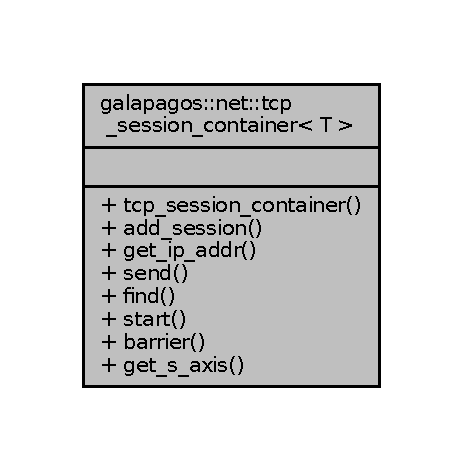
\includegraphics[width=222pt]{classgalapagos_1_1net_1_1tcp__session__container__coll__graph}
\end{center}
\end{figure}
\subsection*{Public Member Functions}
\begin{DoxyCompactItemize}
\item 
\hyperlink{classgalapagos_1_1net_1_1tcp__session__container_aff7a9dd66971b6812b9de462d588cc95}{tcp\+\_\+session\+\_\+container} (std\+::vector$<$ std\+::string $>$ \&\+\_\+kernel\+\_\+info\+\_\+table, std\+::string \&\hyperlink{test_8cpp_ad6c70ba8571527f1543822ce71b9a109}{my\+\_\+address}, \hyperlink{classgalapagos_1_1done__clean}{done\+\_\+clean} $\ast$\+\_\+dc, \hyperlink{classgalapagos_1_1n__to__one__router}{n\+\_\+to\+\_\+one\+\_\+router}$<$ \hyperlink{test_8cpp_a0658ceffa730c765d449bb3d21871b5f}{T} $>$ $\ast$\+\_\+router\+\_\+out, std\+::mutex $\ast$\+\_\+mutex\+\_\+packets\+\_\+in\+\_\+flight, int $\ast$\+\_\+packets\+\_\+in\+\_\+flight)
\item 
void \hyperlink{classgalapagos_1_1net_1_1tcp__session__container_ad1c38390da6df1bdd61d3c6801edd3c1}{add\+\_\+session} (boost\+::asio\+::ip\+::tcp\+::socket \+\_\+socket, boost\+::asio\+::io\+\_\+context $\ast$io\+\_\+context)
\item 
std\+::string \hyperlink{classgalapagos_1_1net_1_1tcp__session__container_a28211ba6529ca572b94169740416fb22}{get\+\_\+ip\+\_\+addr} (short dest)
\item 
bool \hyperlink{classgalapagos_1_1net_1_1tcp__session__container_a361a7a20068ba7341626863f05316602}{send} (std\+::string ip\+\_\+addr, char $\ast$data, int size, short dest, short src)
\item 
bool \hyperlink{classgalapagos_1_1net_1_1tcp__session__container_a176b5612e91affbb36ef59dcab13c011}{find} (std\+::string \+\_\+ip\+\_\+addr)
\item 
void \hyperlink{classgalapagos_1_1net_1_1tcp__session__container_aa180bb49b25f7987575dd00475ce00c5}{start} ()
\item 
bool \hyperlink{classgalapagos_1_1net_1_1tcp__session__container_a7c516c69d30b370dea139ede11d85187}{barrier} ()
\item 
\hyperlink{classgalapagos_1_1interface}{interface}$<$ \hyperlink{test_8cpp_a0658ceffa730c765d449bb3d21871b5f}{T} $>$ $\ast$ \hyperlink{classgalapagos_1_1net_1_1tcp__session__container_a6fb1b0b779f28ea29825eb6bd96fa66a}{get\+\_\+s\+\_\+axis} (std\+::string ip\+\_\+addr)
\end{DoxyCompactItemize}


\subsection{Detailed Description}
\subsubsection*{template$<$class T$>$\\*
class galapagos\+::net\+::tcp\+\_\+session\+\_\+container$<$ T $>$}

Class for the session\+\_\+container. Addressable by dest. 

Vector of sessions, addressable by dest. Contains helping functions that can help address sessions by ip\+\_\+addrs. Allows user to send data into session and has router to arbitrate from m\+\_\+axis of each session to the output. \begin{DoxyAuthor}{Author}
Naif Tarafdar 
\end{DoxyAuthor}
\begin{DoxyDate}{Date}
April 20, 2019 
\end{DoxyDate}


\subsection{Constructor \& Destructor Documentation}
\index{galapagos\+::net\+::tcp\+\_\+session\+\_\+container@{galapagos\+::net\+::tcp\+\_\+session\+\_\+container}!tcp\+\_\+session\+\_\+container@{tcp\+\_\+session\+\_\+container}}
\index{tcp\+\_\+session\+\_\+container@{tcp\+\_\+session\+\_\+container}!galapagos\+::net\+::tcp\+\_\+session\+\_\+container@{galapagos\+::net\+::tcp\+\_\+session\+\_\+container}}
\subsubsection[{\texorpdfstring{tcp\+\_\+session\+\_\+container(std\+::vector$<$ std\+::string $>$ \&\+\_\+kernel\+\_\+info\+\_\+table, std\+::string \&my\+\_\+address, done\+\_\+clean $\ast$\+\_\+dc, n\+\_\+to\+\_\+one\+\_\+router$<$ T $>$ $\ast$\+\_\+router\+\_\+out, std\+::mutex $\ast$\+\_\+mutex\+\_\+packets\+\_\+in\+\_\+flight, int $\ast$\+\_\+packets\+\_\+in\+\_\+flight)}{tcp_session_container(std::vector< std::string > &_kernel_info_table, std::string &my_address, done_clean *_dc, n_to_one_router< T > *_router_out, std::mutex *_mutex_packets_in_flight, int *_packets_in_flight)}}]{\setlength{\rightskip}{0pt plus 5cm}template$<$class T $>$ tcp\+\_\+session\+\_\+container\+::tcp\+\_\+session\+\_\+container (
\begin{DoxyParamCaption}
\item[{std\+::vector$<$ std\+::string $>$ \&}]{\+\_\+kernel\+\_\+info\+\_\+table, }
\item[{std\+::string \&}]{my\+\_\+address, }
\item[{{\bf galapagos\+::done\+\_\+clean} $\ast$}]{\+\_\+dc, }
\item[{{\bf galapagos\+::n\+\_\+to\+\_\+one\+\_\+router}$<$ {\bf T} $>$ $\ast$}]{\+\_\+router\+\_\+out, }
\item[{std\+::mutex $\ast$}]{\+\_\+mutex\+\_\+packets\+\_\+in\+\_\+flight, }
\item[{int $\ast$}]{\+\_\+packets\+\_\+in\+\_\+flight}
\end{DoxyParamCaption}
)}\hypertarget{classgalapagos_1_1net_1_1tcp__session__container_aff7a9dd66971b6812b9de462d588cc95}{}\label{classgalapagos_1_1net_1_1tcp__session__container_aff7a9dd66971b6812b9de462d588cc95}


\subsection{Member Function Documentation}
\index{galapagos\+::net\+::tcp\+\_\+session\+\_\+container@{galapagos\+::net\+::tcp\+\_\+session\+\_\+container}!add\+\_\+session@{add\+\_\+session}}
\index{add\+\_\+session@{add\+\_\+session}!galapagos\+::net\+::tcp\+\_\+session\+\_\+container@{galapagos\+::net\+::tcp\+\_\+session\+\_\+container}}
\subsubsection[{\texorpdfstring{add\+\_\+session(boost\+::asio\+::ip\+::tcp\+::socket \+\_\+socket, boost\+::asio\+::io\+\_\+context $\ast$io\+\_\+context)}{add_session(boost::asio::ip::tcp::socket _socket, boost::asio::io_context *io_context)}}]{\setlength{\rightskip}{0pt plus 5cm}template$<$class T $>$ void tcp\+\_\+session\+\_\+container\+::add\+\_\+session (
\begin{DoxyParamCaption}
\item[{boost\+::asio\+::ip\+::tcp\+::socket}]{\+\_\+socket, }
\item[{boost\+::asio\+::io\+\_\+context $\ast$}]{io\+\_\+context}
\end{DoxyParamCaption}
)}\hypertarget{classgalapagos_1_1net_1_1tcp__session__container_ad1c38390da6df1bdd61d3c6801edd3c1}{}\label{classgalapagos_1_1net_1_1tcp__session__container_ad1c38390da6df1bdd61d3c6801edd3c1}
Adds a new session of a particular socket 
\begin{DoxyTemplParams}{Template Parameters}
{\em T} & the type of data used within each galapagos packet (default ap\+\_\+uint$<$64$>$) \\
\hline
\end{DoxyTemplParams}

\begin{DoxyParams}[1]{Parameters}
\mbox{\tt in}  & {\em \+\_\+socket} & tcp socket that has been made and moved into session \\
\hline
\mbox{\tt in}  & {\em \+\_\+io\+\_\+context} & pointer to io\+\_\+context needed to communicate over socket \\
\hline
\end{DoxyParams}
\index{galapagos\+::net\+::tcp\+\_\+session\+\_\+container@{galapagos\+::net\+::tcp\+\_\+session\+\_\+container}!barrier@{barrier}}
\index{barrier@{barrier}!galapagos\+::net\+::tcp\+\_\+session\+\_\+container@{galapagos\+::net\+::tcp\+\_\+session\+\_\+container}}
\subsubsection[{\texorpdfstring{barrier()}{barrier()}}]{\setlength{\rightskip}{0pt plus 5cm}template$<$class T$>$ bool {\bf galapagos\+::net\+::tcp\+\_\+session\+\_\+container}$<$ {\bf T} $>$\+::barrier (
\begin{DoxyParamCaption}
{}
\end{DoxyParamCaption}
)}\hypertarget{classgalapagos_1_1net_1_1tcp__session__container_a7c516c69d30b370dea139ede11d85187}{}\label{classgalapagos_1_1net_1_1tcp__session__container_a7c516c69d30b370dea139ede11d85187}
\index{galapagos\+::net\+::tcp\+\_\+session\+\_\+container@{galapagos\+::net\+::tcp\+\_\+session\+\_\+container}!find@{find}}
\index{find@{find}!galapagos\+::net\+::tcp\+\_\+session\+\_\+container@{galapagos\+::net\+::tcp\+\_\+session\+\_\+container}}
\subsubsection[{\texorpdfstring{find(std\+::string \+\_\+ip\+\_\+addr)}{find(std::string _ip_addr)}}]{\setlength{\rightskip}{0pt plus 5cm}template$<$class T $>$ bool tcp\+\_\+session\+\_\+container\+::find (
\begin{DoxyParamCaption}
\item[{std\+::string}]{\+\_\+ip\+\_\+addr}
\end{DoxyParamCaption}
)}\hypertarget{classgalapagos_1_1net_1_1tcp__session__container_a176b5612e91affbb36ef59dcab13c011}{}\label{classgalapagos_1_1net_1_1tcp__session__container_a176b5612e91affbb36ef59dcab13c011}
Checks if a session exists with ip\+\_\+addr 
\begin{DoxyTemplParams}{Template Parameters}
{\em T} & the type of data used within each galapagos packet (default ap\+\_\+uint$<$64$>$) \\
\hline
\end{DoxyTemplParams}
\begin{DoxyReturn}{Returns}
if session with ip\+\_\+addr exists 
\end{DoxyReturn}
\index{galapagos\+::net\+::tcp\+\_\+session\+\_\+container@{galapagos\+::net\+::tcp\+\_\+session\+\_\+container}!get\+\_\+ip\+\_\+addr@{get\+\_\+ip\+\_\+addr}}
\index{get\+\_\+ip\+\_\+addr@{get\+\_\+ip\+\_\+addr}!galapagos\+::net\+::tcp\+\_\+session\+\_\+container@{galapagos\+::net\+::tcp\+\_\+session\+\_\+container}}
\subsubsection[{\texorpdfstring{get\+\_\+ip\+\_\+addr(short dest)}{get_ip_addr(short dest)}}]{\setlength{\rightskip}{0pt plus 5cm}template$<$class T $>$ std\+::string tcp\+\_\+session\+\_\+container\+::get\+\_\+ip\+\_\+addr (
\begin{DoxyParamCaption}
\item[{short}]{dest}
\end{DoxyParamCaption}
)}\hypertarget{classgalapagos_1_1net_1_1tcp__session__container_a28211ba6529ca572b94169740416fb22}{}\label{classgalapagos_1_1net_1_1tcp__session__container_a28211ba6529ca572b94169740416fb22}
Gets ip\+\_\+addr of kern dest 
\begin{DoxyTemplParams}{Template Parameters}
{\em T} & the type of data used within each galapagos packet (default ap\+\_\+uint$<$64$>$) \\
\hline
\end{DoxyTemplParams}
\begin{DoxyReturn}{Returns}
ip\+\_\+addr 
\end{DoxyReturn}
\index{galapagos\+::net\+::tcp\+\_\+session\+\_\+container@{galapagos\+::net\+::tcp\+\_\+session\+\_\+container}!get\+\_\+s\+\_\+axis@{get\+\_\+s\+\_\+axis}}
\index{get\+\_\+s\+\_\+axis@{get\+\_\+s\+\_\+axis}!galapagos\+::net\+::tcp\+\_\+session\+\_\+container@{galapagos\+::net\+::tcp\+\_\+session\+\_\+container}}
\subsubsection[{\texorpdfstring{get\+\_\+s\+\_\+axis(std\+::string ip\+\_\+addr)}{get_s_axis(std::string ip_addr)}}]{\setlength{\rightskip}{0pt plus 5cm}template$<$class T $>$ {\bf galapagos\+::interface}$<$ {\bf T} $>$ $\ast$ tcp\+\_\+session\+\_\+container\+::get\+\_\+s\+\_\+axis (
\begin{DoxyParamCaption}
\item[{std\+::string}]{ip\+\_\+addr}
\end{DoxyParamCaption}
)}\hypertarget{classgalapagos_1_1net_1_1tcp__session__container_a6fb1b0b779f28ea29825eb6bd96fa66a}{}\label{classgalapagos_1_1net_1_1tcp__session__container_a6fb1b0b779f28ea29825eb6bd96fa66a}
Gets input interface of a session 
\begin{DoxyTemplParams}{Template Parameters}
{\em T} & the type of data used within each galapagos packet (default ap\+\_\+uint$<$64$>$) \\
\hline
\end{DoxyTemplParams}

\begin{DoxyParams}[1]{Parameters}
\mbox{\tt in}  & {\em ip\+\_\+addr} & session indexed by ip\+\_\+addr \\
\hline
\end{DoxyParams}
\begin{DoxyReturn}{Returns}
pointer of input interface 
\end{DoxyReturn}
\index{galapagos\+::net\+::tcp\+\_\+session\+\_\+container@{galapagos\+::net\+::tcp\+\_\+session\+\_\+container}!send@{send}}
\index{send@{send}!galapagos\+::net\+::tcp\+\_\+session\+\_\+container@{galapagos\+::net\+::tcp\+\_\+session\+\_\+container}}
\subsubsection[{\texorpdfstring{send(std\+::string ip\+\_\+addr, char $\ast$data, int size, short dest, short src)}{send(std::string ip_addr, char *data, int size, short dest, short src)}}]{\setlength{\rightskip}{0pt plus 5cm}template$<$class T$>$ bool {\bf galapagos\+::net\+::tcp\+\_\+session\+\_\+container}$<$ {\bf T} $>$\+::send (
\begin{DoxyParamCaption}
\item[{std\+::string}]{ip\+\_\+addr, }
\item[{char $\ast$}]{data, }
\item[{int}]{size, }
\item[{short}]{dest, }
\item[{short}]{src}
\end{DoxyParamCaption}
)}\hypertarget{classgalapagos_1_1net_1_1tcp__session__container_a361a7a20068ba7341626863f05316602}{}\label{classgalapagos_1_1net_1_1tcp__session__container_a361a7a20068ba7341626863f05316602}
\index{galapagos\+::net\+::tcp\+\_\+session\+\_\+container@{galapagos\+::net\+::tcp\+\_\+session\+\_\+container}!start@{start}}
\index{start@{start}!galapagos\+::net\+::tcp\+\_\+session\+\_\+container@{galapagos\+::net\+::tcp\+\_\+session\+\_\+container}}
\subsubsection[{\texorpdfstring{start()}{start()}}]{\setlength{\rightskip}{0pt plus 5cm}template$<$class T$>$ void {\bf galapagos\+::net\+::tcp\+\_\+session\+\_\+container}$<$ {\bf T} $>$\+::start (
\begin{DoxyParamCaption}
{}
\end{DoxyParamCaption}
)}\hypertarget{classgalapagos_1_1net_1_1tcp__session__container_aa180bb49b25f7987575dd00475ce00c5}{}\label{classgalapagos_1_1net_1_1tcp__session__container_aa180bb49b25f7987575dd00475ce00c5}


The documentation for this class was generated from the following file\+:\begin{DoxyCompactItemize}
\item 
\hyperlink{galapagos__net__tcp__session_8hpp}{galapagos\+\_\+net\+\_\+tcp\+\_\+session.\+hpp}\end{DoxyCompactItemize}

\hypertarget{classgalapagos_1_1net_1_1udp}{}\section{galapagos\+:\+:net\+:\+:udp$<$ T $>$ Class Template Reference}
\label{classgalapagos_1_1net_1_1udp}\index{galapagos\+::net\+::udp$<$ T $>$@{galapagos\+::net\+::udp$<$ T $>$}}


Class udp driver.  




{\ttfamily \#include $<$galapagos\+\_\+net\+\_\+udp.\+hpp$>$}



Inheritance diagram for galapagos\+:\+:net\+:\+:udp$<$ T $>$\+:
\nopagebreak
\begin{figure}[H]
\begin{center}
\leavevmode
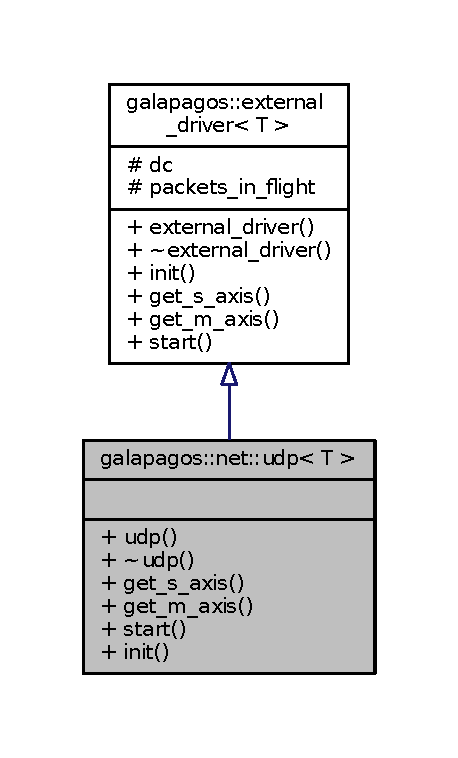
\includegraphics[width=220pt]{classgalapagos_1_1net_1_1udp__inherit__graph}
\end{center}
\end{figure}


Collaboration diagram for galapagos\+:\+:net\+:\+:udp$<$ T $>$\+:
\nopagebreak
\begin{figure}[H]
\begin{center}
\leavevmode
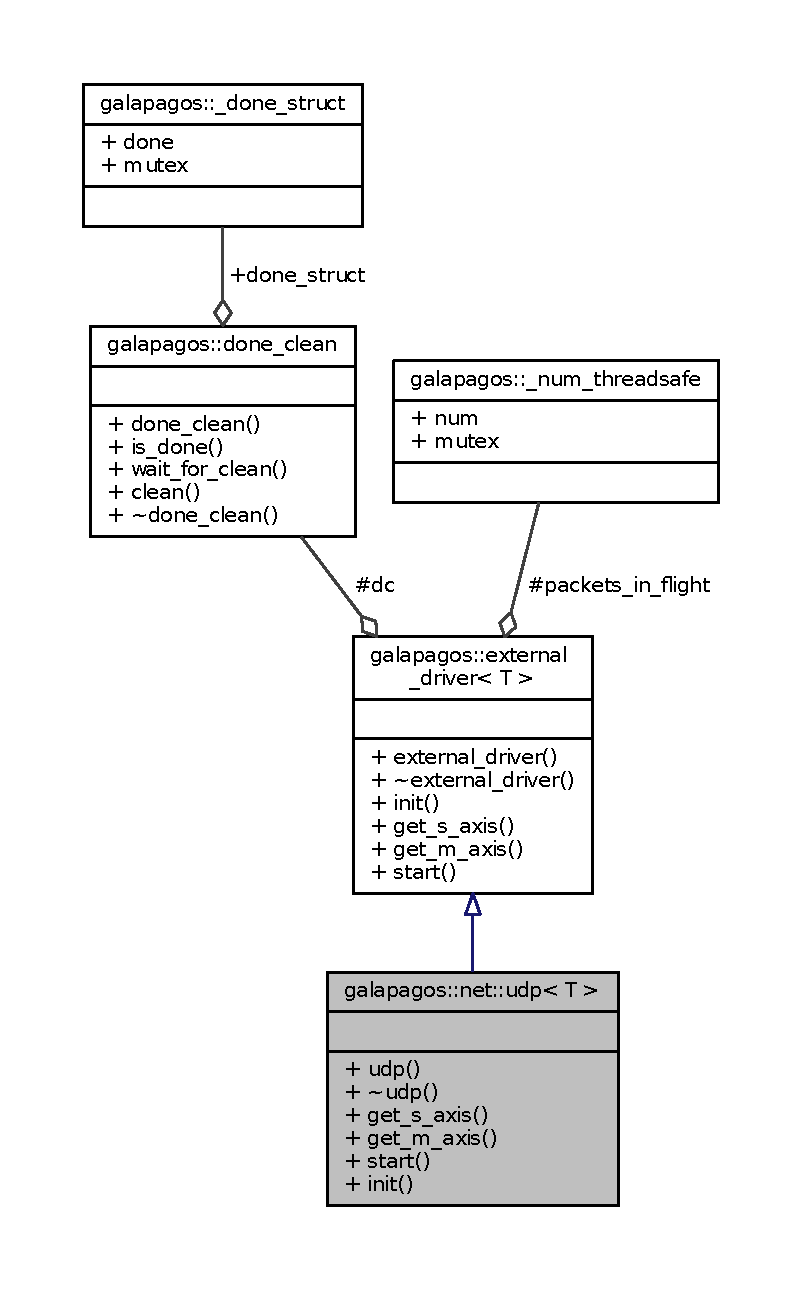
\includegraphics[height=550pt]{classgalapagos_1_1net_1_1udp__coll__graph}
\end{center}
\end{figure}
\subsection*{Public Member Functions}
\begin{DoxyCompactItemize}
\item 
\hyperlink{classgalapagos_1_1net_1_1udp_a86de3f3b1ca57dbb7914062f5424ab6d}{udp} (short port, std\+::vector$<$ std\+::string $>$ kern\+\_\+info\+\_\+table, std\+::string my\+\_\+address)
\item 
\hyperlink{classgalapagos_1_1net_1_1udp_a9f39e94af7950e82bd86a8ae08724132}{$\sim$udp} ()
\item 
\hyperlink{classgalapagos_1_1interface}{interface}$<$ \hyperlink{test_8cpp_a0658ceffa730c765d449bb3d21871b5f}{T} $>$ $\ast$ \hyperlink{classgalapagos_1_1net_1_1udp_aed1c1ca798141a5eb83382b384ede0c1}{get\+\_\+s\+\_\+axis} ()
\item 
\hyperlink{classgalapagos_1_1interface}{interface}$<$ \hyperlink{test_8cpp_a0658ceffa730c765d449bb3d21871b5f}{T} $>$ $\ast$ \hyperlink{classgalapagos_1_1net_1_1udp_a5ab392ec0015391f4428b34463d62d06}{get\+\_\+m\+\_\+axis} ()
\item 
void \hyperlink{classgalapagos_1_1net_1_1udp_acb79ddb76eeb80fbf775cba76f251ac8}{start} ()
\item 
void \hyperlink{classgalapagos_1_1net_1_1udp_a0a071fe7943e7ff4d59640dd39392b50}{init} (\hyperlink{classgalapagos_1_1done__clean}{galapagos\+::done\+\_\+clean} $\ast$, int $\ast$\+\_\+packets\+\_\+in\+\_\+flight, std\+::mutex $\ast$\+\_\+mutex\+\_\+packets\+\_\+in\+\_\+flight)
\end{DoxyCompactItemize}
\subsection*{Additional Inherited Members}


\subsection{Detailed Description}
\subsubsection*{template$<$class T$>$\\*
class galapagos\+::net\+::udp$<$ T $>$}

Class udp driver. 

A software implementation of an n to one router, used by network node to arbitrade output of sessions into the node. Routes between input interfaces(s\+\_\+axis) and an output interface(m\+\_\+axis). \begin{DoxyAuthor}{Author}
Naif Tarafdar 
\end{DoxyAuthor}
\begin{DoxyDate}{Date}
April 20, 2019 
\end{DoxyDate}


\subsection{Constructor \& Destructor Documentation}
\index{galapagos\+::net\+::udp@{galapagos\+::net\+::udp}!udp@{udp}}
\index{udp@{udp}!galapagos\+::net\+::udp@{galapagos\+::net\+::udp}}
\subsubsection[{\texorpdfstring{udp(short port, std\+::vector$<$ std\+::string $>$ kern\+\_\+info\+\_\+table, std\+::string my\+\_\+address)}{udp(short port, std::vector< std::string > kern_info_table, std::string my_address)}}]{\setlength{\rightskip}{0pt plus 5cm}template$<$class T $>$ {\bf galapagos\+::net\+::udp}$<$ {\bf T} $>$\+::{\bf udp} (
\begin{DoxyParamCaption}
\item[{short}]{port, }
\item[{std\+::vector$<$ std\+::string $>$}]{kern\+\_\+info\+\_\+table, }
\item[{std\+::string}]{my\+\_\+address}
\end{DoxyParamCaption}
)}\hypertarget{classgalapagos_1_1net_1_1udp_a86de3f3b1ca57dbb7914062f5424ab6d}{}\label{classgalapagos_1_1net_1_1udp_a86de3f3b1ca57dbb7914062f5424ab6d}
\index{galapagos\+::net\+::udp@{galapagos\+::net\+::udp}!````~udp@{$\sim$udp}}
\index{````~udp@{$\sim$udp}!galapagos\+::net\+::udp@{galapagos\+::net\+::udp}}
\subsubsection[{\texorpdfstring{$\sim$udp()}{~udp()}}]{\setlength{\rightskip}{0pt plus 5cm}template$<$class T $>$ {\bf galapagos\+::net\+::udp}$<$ {\bf T} $>$\+::$\sim${\bf udp} (
\begin{DoxyParamCaption}
{}
\end{DoxyParamCaption}
)\hspace{0.3cm}{\ttfamily [inline]}}\hypertarget{classgalapagos_1_1net_1_1udp_a9f39e94af7950e82bd86a8ae08724132}{}\label{classgalapagos_1_1net_1_1udp_a9f39e94af7950e82bd86a8ae08724132}


\subsection{Member Function Documentation}
\index{galapagos\+::net\+::udp@{galapagos\+::net\+::udp}!get\+\_\+m\+\_\+axis@{get\+\_\+m\+\_\+axis}}
\index{get\+\_\+m\+\_\+axis@{get\+\_\+m\+\_\+axis}!galapagos\+::net\+::udp@{galapagos\+::net\+::udp}}
\subsubsection[{\texorpdfstring{get\+\_\+m\+\_\+axis()}{get_m_axis()}}]{\setlength{\rightskip}{0pt plus 5cm}template$<$class T $>$ {\bf galapagos\+::interface}$<$ {\bf T} $>$ $\ast$ {\bf galapagos\+::net\+::udp}$<$ {\bf T} $>$\+::get\+\_\+m\+\_\+axis (
\begin{DoxyParamCaption}
{}
\end{DoxyParamCaption}
)\hspace{0.3cm}{\ttfamily [virtual]}}\hypertarget{classgalapagos_1_1net_1_1udp_a5ab392ec0015391f4428b34463d62d06}{}\label{classgalapagos_1_1net_1_1udp_a5ab392ec0015391f4428b34463d62d06}


Implements \hyperlink{classgalapagos_1_1external__driver_abc7938fd7247c7404441473da71a357e}{galapagos\+::external\+\_\+driver$<$ T $>$}.

\index{galapagos\+::net\+::udp@{galapagos\+::net\+::udp}!get\+\_\+s\+\_\+axis@{get\+\_\+s\+\_\+axis}}
\index{get\+\_\+s\+\_\+axis@{get\+\_\+s\+\_\+axis}!galapagos\+::net\+::udp@{galapagos\+::net\+::udp}}
\subsubsection[{\texorpdfstring{get\+\_\+s\+\_\+axis()}{get_s_axis()}}]{\setlength{\rightskip}{0pt plus 5cm}template$<$class T $>$ {\bf galapagos\+::interface}$<$ {\bf T} $>$ $\ast$ {\bf galapagos\+::net\+::udp}$<$ {\bf T} $>$\+::get\+\_\+s\+\_\+axis (
\begin{DoxyParamCaption}
{}
\end{DoxyParamCaption}
)\hspace{0.3cm}{\ttfamily [virtual]}}\hypertarget{classgalapagos_1_1net_1_1udp_aed1c1ca798141a5eb83382b384ede0c1}{}\label{classgalapagos_1_1net_1_1udp_aed1c1ca798141a5eb83382b384ede0c1}


Implements \hyperlink{classgalapagos_1_1external__driver_aded446e9ebbdd03b461f336045aa7cd2}{galapagos\+::external\+\_\+driver$<$ T $>$}.

\index{galapagos\+::net\+::udp@{galapagos\+::net\+::udp}!init@{init}}
\index{init@{init}!galapagos\+::net\+::udp@{galapagos\+::net\+::udp}}
\subsubsection[{\texorpdfstring{init(galapagos\+::done\+\_\+clean $\ast$, int $\ast$\+\_\+packets\+\_\+in\+\_\+flight, std\+::mutex $\ast$\+\_\+mutex\+\_\+packets\+\_\+in\+\_\+flight)}{init(galapagos::done_clean *, int *_packets_in_flight, std::mutex *_mutex_packets_in_flight)}}]{\setlength{\rightskip}{0pt plus 5cm}template$<$class T $>$ void {\bf galapagos\+::net\+::udp}$<$ {\bf T} $>$\+::init (
\begin{DoxyParamCaption}
\item[{{\bf galapagos\+::done\+\_\+clean} $\ast$}]{\+\_\+dc, }
\item[{int $\ast$}]{\+\_\+packets\+\_\+in\+\_\+flight, }
\item[{std\+::mutex $\ast$}]{\+\_\+mutex\+\_\+packets\+\_\+in\+\_\+flight}
\end{DoxyParamCaption}
)\hspace{0.3cm}{\ttfamily [virtual]}}\hypertarget{classgalapagos_1_1net_1_1udp_a0a071fe7943e7ff4d59640dd39392b50}{}\label{classgalapagos_1_1net_1_1udp_a0a071fe7943e7ff4d59640dd39392b50}


Implements \hyperlink{classgalapagos_1_1external__driver_ab8b753325b02ee15efe16158cd3fe119}{galapagos\+::external\+\_\+driver$<$ T $>$}.

\index{galapagos\+::net\+::udp@{galapagos\+::net\+::udp}!start@{start}}
\index{start@{start}!galapagos\+::net\+::udp@{galapagos\+::net\+::udp}}
\subsubsection[{\texorpdfstring{start()}{start()}}]{\setlength{\rightskip}{0pt plus 5cm}template$<$class T $>$ void {\bf galapagos\+::net\+::udp}$<$ {\bf T} $>$\+::start (
\begin{DoxyParamCaption}
{}
\end{DoxyParamCaption}
)\hspace{0.3cm}{\ttfamily [virtual]}}\hypertarget{classgalapagos_1_1net_1_1udp_acb79ddb76eeb80fbf775cba76f251ac8}{}\label{classgalapagos_1_1net_1_1udp_acb79ddb76eeb80fbf775cba76f251ac8}


Implements \hyperlink{classgalapagos_1_1external__driver_a7eacf72788a4ce6976499e36f1b7b3a6}{galapagos\+::external\+\_\+driver$<$ T $>$}.



The documentation for this class was generated from the following file\+:\begin{DoxyCompactItemize}
\item 
\hyperlink{galapagos__net__udp_8hpp}{galapagos\+\_\+net\+\_\+udp.\+hpp}\end{DoxyCompactItemize}

\chapter{File Documentation}
\hypertarget{benchmark__0_8cpp}{}\section{benchmark\+\_\+0.\+cpp File Reference}
\label{benchmark__0_8cpp}\index{benchmark\+\_\+0.\+cpp@{benchmark\+\_\+0.\+cpp}}
{\ttfamily \#include $<$string$>$}\\*
{\ttfamily \#include $<$vector$>$}\\*
{\ttfamily \#include \char`\"{}galapagos\+\_\+interface.\+hpp\char`\"{}}\\*
{\ttfamily \#include \char`\"{}galapagos\+\_\+node.\+hpp\char`\"{}}\\*
{\ttfamily \#include \char`\"{}galapagos\+\_\+net\+\_\+tcp.\+hpp\char`\"{}}\\*
Include dependency graph for benchmark\+\_\+0.\+cpp\+:
\nopagebreak
\begin{figure}[H]
\begin{center}
\leavevmode
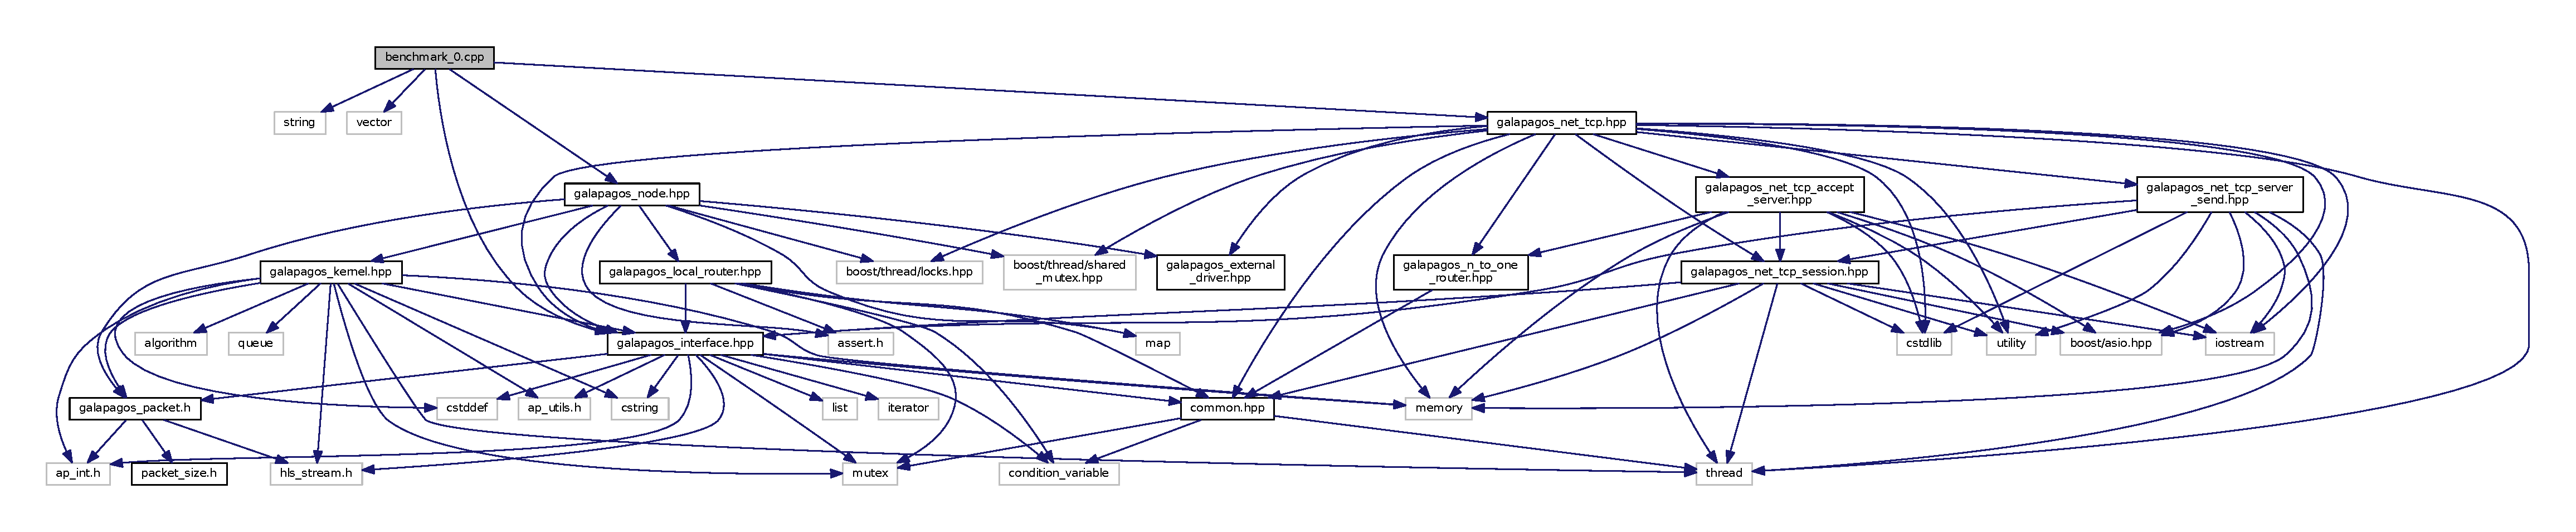
\includegraphics[width=350pt]{benchmark__0_8cpp__incl}
\end{center}
\end{figure}
\subsection*{Classes}
\begin{DoxyCompactItemize}
\item 
class \hyperlink{classmy__barrier}{my\+\_\+barrier}
\end{DoxyCompactItemize}
\subsection*{Macros}
\begin{DoxyCompactItemize}
\item 
\#define \hyperlink{benchmark__0_8cpp_ab3be0641eb76161a48ed528e6eea2ac3}{N\+U\+M\+\_\+\+I\+T\+E\+R\+A\+T\+I\+O\+NS}~100000
\end{DoxyCompactItemize}
\subsection*{Functions}
\begin{DoxyCompactItemize}
\item 
void \hyperlink{benchmark__0_8cpp_a952c103146dc9b79782931ba3fa131f1}{generate\+\_\+flit} (int iterations, int size, int id, int dest, \hyperlink{galapagos__interface_8hpp_af5070d0f7a016a7cd5677cdf2e30ac63}{galapagos\+\_\+interface} $\ast$out)
\item 
auto \hyperlink{benchmark__0_8cpp_afc8eb6b6cadc5c14cdf86a742ee312a9}{start\+\_\+timer} ()
\item 
void \hyperlink{benchmark__0_8cpp_adb55cd51f1bde00069b064101c60d86f}{print\+\_\+time} (std\+::chrono\+::high\+\_\+resolution\+\_\+clock\+::time\+\_\+point timer, std\+::string label)
\item 
void \hyperlink{benchmark__0_8cpp_a54f037e7a8d79a8557a33713c97c3ed8}{generate\+\_\+packet} (int iterations, int size, int id, int dest, \hyperlink{galapagos__interface_8hpp_af5070d0f7a016a7cd5677cdf2e30ac63}{galapagos\+\_\+interface} $\ast$out)
\item 
void \hyperlink{benchmark__0_8cpp_a79daffd29405a76f0c0676b577e2843d}{generate\+\_\+packet} (char $\ast$mem, int iterations, int size, int id, int dest, \hyperlink{galapagos__interface_8hpp_af5070d0f7a016a7cd5677cdf2e30ac63}{galapagos\+\_\+interface} $\ast$out)
\item 
void \hyperlink{benchmark__0_8cpp_a83fe9f71488e293cfe12208b9a4b082a}{generate\+\_\+packet} (std\+::vector$<$ ap\+\_\+uint$<$ 64 $>$ $>$ $\ast$vec, int iterations, int size, int id, int dest, \hyperlink{galapagos__interface_8hpp_af5070d0f7a016a7cd5677cdf2e30ac63}{galapagos\+\_\+interface} $\ast$out)
\item 
void \hyperlink{benchmark__0_8cpp_ab58f1ce436d790a26a5c52969cb832aa}{receive\+\_\+flit\+\_\+perf} (int iterations, int size, \hyperlink{galapagos__interface_8hpp_af5070d0f7a016a7cd5677cdf2e30ac63}{galapagos\+\_\+interface} $\ast$in)
\item 
void \hyperlink{benchmark__0_8cpp_affc065c5706e3d2766ff79d86064eba6}{receive\+\_\+packet\+\_\+perf} (int iterations, int size, \hyperlink{galapagos__interface_8hpp_af5070d0f7a016a7cd5677cdf2e30ac63}{galapagos\+\_\+interface} $\ast$in)
\item 
void \hyperlink{benchmark__0_8cpp_a5d0cd200435e0f644ecd4f7b8acf04fb}{receive\+\_\+packet\+\_\+mem\+\_\+perf} (char $\ast$mem, int iterations, int size, \hyperlink{galapagos__interface_8hpp_af5070d0f7a016a7cd5677cdf2e30ac63}{galapagos\+\_\+interface} $\ast$in)
\item 
void \hyperlink{benchmark__0_8cpp_abe8edb4407293362836700570a97a10b}{print\+\_\+throughput} (std\+::string test\+\_\+name, std\+::string test\+\_\+type, int size)
\item 
void \hyperlink{benchmark__0_8cpp_aec791ee0f05029c542c54c2b12fd4e2e}{print\+\_\+latency} (std\+::string test\+\_\+name, std\+::string test\+\_\+type, int size, std\+::chrono\+::duration$<$ double $>$ diff)
\item 
void \hyperlink{benchmark__0_8cpp_a06e3b5fe38c1f4cb5972629ceef904ae}{kern\+\_\+benchmark\+\_\+0} (short id, \hyperlink{galapagos__interface_8hpp_af5070d0f7a016a7cd5677cdf2e30ac63}{galapagos\+\_\+interface} $\ast$in, \hyperlink{galapagos__interface_8hpp_af5070d0f7a016a7cd5677cdf2e30ac63}{galapagos\+\_\+interface} $\ast$out)
\item 
void \hyperlink{benchmark__0_8cpp_ac38d2162e8da4504b111ec67227640dc}{kern\+\_\+benchmark\+\_\+1} (short id, \hyperlink{galapagos__interface_8hpp_af5070d0f7a016a7cd5677cdf2e30ac63}{galapagos\+\_\+interface} $\ast$in, \hyperlink{galapagos__interface_8hpp_af5070d0f7a016a7cd5677cdf2e30ac63}{galapagos\+\_\+interface} $\ast$out)
\item 
void \hyperlink{benchmark__0_8cpp_a76beaf69aae21f9337aeebc261611e58}{kern\+\_\+benchmark\+\_\+reply\+\_\+0} (short id, \hyperlink{galapagos__interface_8hpp_af5070d0f7a016a7cd5677cdf2e30ac63}{galapagos\+\_\+interface} $\ast$in, \hyperlink{galapagos__interface_8hpp_af5070d0f7a016a7cd5677cdf2e30ac63}{galapagos\+\_\+interface} $\ast$out)
\item 
int \hyperlink{benchmark__0_8cpp_ae66f6b31b5ad750f1fe042a706a4e3d4}{main} ()
\end{DoxyCompactItemize}
\subsection*{Variables}
\begin{DoxyCompactItemize}
\item 
std\+::chrono\+::time\+\_\+point$<$ std\+::chrono\+::high\+\_\+resolution\+\_\+clock $>$ \hyperlink{benchmark__0_8cpp_a46dea58f2d527f376090214bd5c3233d}{start}
\item 
std\+::chrono\+::time\+\_\+point$<$ std\+::chrono\+::high\+\_\+resolution\+\_\+clock $>$ \hyperlink{benchmark__0_8cpp_ace54cb99b52f35f3a98f99e2a75dd5ad}{end}
\item 
\hyperlink{classmy__barrier}{my\+\_\+barrier} \hyperlink{benchmark__0_8cpp_aff51f609cca9859fa4931f4e40a3f9c1}{barrier} (2)
\item 
int \hyperlink{benchmark__0_8cpp_a242878592db6f7a2c418597075681ef7}{msg\+\_\+num} = 11
\item 
int \hyperlink{benchmark__0_8cpp_aba50ac03860735a8b607b2fcbf57dc60}{msg\+\_\+size} \mbox{[}$\,$\mbox{]} = \{1, 2, 4, 8, 16, 32, 64, 128, 256, 512, \hyperlink{galapagos__interface_8hpp_a1d5dab30b404fab91608086105afc78c}{M\+A\+X\+\_\+\+B\+U\+F\+F\+ER}\}
\item 
int \hyperlink{benchmark__0_8cpp_a9d85b8fff6f70aa502b3c74d38c02ded}{msg\+\_\+reply} = 2
\end{DoxyCompactItemize}


\subsection{Macro Definition Documentation}
\index{benchmark\+\_\+0.\+cpp@{benchmark\+\_\+0.\+cpp}!N\+U\+M\+\_\+\+I\+T\+E\+R\+A\+T\+I\+O\+NS@{N\+U\+M\+\_\+\+I\+T\+E\+R\+A\+T\+I\+O\+NS}}
\index{N\+U\+M\+\_\+\+I\+T\+E\+R\+A\+T\+I\+O\+NS@{N\+U\+M\+\_\+\+I\+T\+E\+R\+A\+T\+I\+O\+NS}!benchmark\+\_\+0.\+cpp@{benchmark\+\_\+0.\+cpp}}
\subsubsection[{\texorpdfstring{N\+U\+M\+\_\+\+I\+T\+E\+R\+A\+T\+I\+O\+NS}{NUM_ITERATIONS}}]{\setlength{\rightskip}{0pt plus 5cm}\#define N\+U\+M\+\_\+\+I\+T\+E\+R\+A\+T\+I\+O\+NS~100000}\hypertarget{benchmark__0_8cpp_ab3be0641eb76161a48ed528e6eea2ac3}{}\label{benchmark__0_8cpp_ab3be0641eb76161a48ed528e6eea2ac3}


\subsection{Function Documentation}
\index{benchmark\+\_\+0.\+cpp@{benchmark\+\_\+0.\+cpp}!generate\+\_\+flit@{generate\+\_\+flit}}
\index{generate\+\_\+flit@{generate\+\_\+flit}!benchmark\+\_\+0.\+cpp@{benchmark\+\_\+0.\+cpp}}
\subsubsection[{\texorpdfstring{generate\+\_\+flit(int iterations, int size, int id, int dest, galapagos\+\_\+interface $\ast$out)}{generate_flit(int iterations, int size, int id, int dest, galapagos_interface *out)}}]{\setlength{\rightskip}{0pt plus 5cm}void generate\+\_\+flit (
\begin{DoxyParamCaption}
\item[{int}]{iterations, }
\item[{int}]{size, }
\item[{int}]{id, }
\item[{int}]{dest, }
\item[{{\bf galapagos\+\_\+interface} $\ast$}]{out}
\end{DoxyParamCaption}
)}\hypertarget{benchmark__0_8cpp_a952c103146dc9b79782931ba3fa131f1}{}\label{benchmark__0_8cpp_a952c103146dc9b79782931ba3fa131f1}
\index{benchmark\+\_\+0.\+cpp@{benchmark\+\_\+0.\+cpp}!generate\+\_\+packet@{generate\+\_\+packet}}
\index{generate\+\_\+packet@{generate\+\_\+packet}!benchmark\+\_\+0.\+cpp@{benchmark\+\_\+0.\+cpp}}
\subsubsection[{\texorpdfstring{generate\+\_\+packet(int iterations, int size, int id, int dest, galapagos\+\_\+interface $\ast$out)}{generate_packet(int iterations, int size, int id, int dest, galapagos_interface *out)}}]{\setlength{\rightskip}{0pt plus 5cm}void generate\+\_\+packet (
\begin{DoxyParamCaption}
\item[{int}]{iterations, }
\item[{int}]{size, }
\item[{int}]{id, }
\item[{int}]{dest, }
\item[{{\bf galapagos\+\_\+interface} $\ast$}]{out}
\end{DoxyParamCaption}
)}\hypertarget{benchmark__0_8cpp_a54f037e7a8d79a8557a33713c97c3ed8}{}\label{benchmark__0_8cpp_a54f037e7a8d79a8557a33713c97c3ed8}
\index{benchmark\+\_\+0.\+cpp@{benchmark\+\_\+0.\+cpp}!generate\+\_\+packet@{generate\+\_\+packet}}
\index{generate\+\_\+packet@{generate\+\_\+packet}!benchmark\+\_\+0.\+cpp@{benchmark\+\_\+0.\+cpp}}
\subsubsection[{\texorpdfstring{generate\+\_\+packet(char $\ast$mem, int iterations, int size, int id, int dest, galapagos\+\_\+interface $\ast$out)}{generate_packet(char *mem, int iterations, int size, int id, int dest, galapagos_interface *out)}}]{\setlength{\rightskip}{0pt plus 5cm}void generate\+\_\+packet (
\begin{DoxyParamCaption}
\item[{char $\ast$}]{mem, }
\item[{int}]{iterations, }
\item[{int}]{size, }
\item[{int}]{id, }
\item[{int}]{dest, }
\item[{{\bf galapagos\+\_\+interface} $\ast$}]{out}
\end{DoxyParamCaption}
)}\hypertarget{benchmark__0_8cpp_a79daffd29405a76f0c0676b577e2843d}{}\label{benchmark__0_8cpp_a79daffd29405a76f0c0676b577e2843d}
\index{benchmark\+\_\+0.\+cpp@{benchmark\+\_\+0.\+cpp}!generate\+\_\+packet@{generate\+\_\+packet}}
\index{generate\+\_\+packet@{generate\+\_\+packet}!benchmark\+\_\+0.\+cpp@{benchmark\+\_\+0.\+cpp}}
\subsubsection[{\texorpdfstring{generate\+\_\+packet(std\+::vector$<$ ap\+\_\+uint$<$ 64 $>$ $>$ $\ast$vec, int iterations, int size, int id, int dest, galapagos\+\_\+interface $\ast$out)}{generate_packet(std::vector< ap_uint< 64 > > *vec, int iterations, int size, int id, int dest, galapagos_interface *out)}}]{\setlength{\rightskip}{0pt plus 5cm}void generate\+\_\+packet (
\begin{DoxyParamCaption}
\item[{std\+::vector$<$ ap\+\_\+uint$<$ 64 $>$ $>$ $\ast$}]{vec, }
\item[{int}]{iterations, }
\item[{int}]{size, }
\item[{int}]{id, }
\item[{int}]{dest, }
\item[{{\bf galapagos\+\_\+interface} $\ast$}]{out}
\end{DoxyParamCaption}
)}\hypertarget{benchmark__0_8cpp_a83fe9f71488e293cfe12208b9a4b082a}{}\label{benchmark__0_8cpp_a83fe9f71488e293cfe12208b9a4b082a}
\index{benchmark\+\_\+0.\+cpp@{benchmark\+\_\+0.\+cpp}!kern\+\_\+benchmark\+\_\+0@{kern\+\_\+benchmark\+\_\+0}}
\index{kern\+\_\+benchmark\+\_\+0@{kern\+\_\+benchmark\+\_\+0}!benchmark\+\_\+0.\+cpp@{benchmark\+\_\+0.\+cpp}}
\subsubsection[{\texorpdfstring{kern\+\_\+benchmark\+\_\+0(short id, galapagos\+\_\+interface $\ast$in, galapagos\+\_\+interface $\ast$out)}{kern_benchmark_0(short id, galapagos_interface *in, galapagos_interface *out)}}]{\setlength{\rightskip}{0pt plus 5cm}void kern\+\_\+benchmark\+\_\+0 (
\begin{DoxyParamCaption}
\item[{short}]{id, }
\item[{{\bf galapagos\+\_\+interface} $\ast$}]{in, }
\item[{{\bf galapagos\+\_\+interface} $\ast$}]{out}
\end{DoxyParamCaption}
)}\hypertarget{benchmark__0_8cpp_a06e3b5fe38c1f4cb5972629ceef904ae}{}\label{benchmark__0_8cpp_a06e3b5fe38c1f4cb5972629ceef904ae}
\index{benchmark\+\_\+0.\+cpp@{benchmark\+\_\+0.\+cpp}!kern\+\_\+benchmark\+\_\+1@{kern\+\_\+benchmark\+\_\+1}}
\index{kern\+\_\+benchmark\+\_\+1@{kern\+\_\+benchmark\+\_\+1}!benchmark\+\_\+0.\+cpp@{benchmark\+\_\+0.\+cpp}}
\subsubsection[{\texorpdfstring{kern\+\_\+benchmark\+\_\+1(short id, galapagos\+\_\+interface $\ast$in, galapagos\+\_\+interface $\ast$out)}{kern_benchmark_1(short id, galapagos_interface *in, galapagos_interface *out)}}]{\setlength{\rightskip}{0pt plus 5cm}void kern\+\_\+benchmark\+\_\+1 (
\begin{DoxyParamCaption}
\item[{short}]{id, }
\item[{{\bf galapagos\+\_\+interface} $\ast$}]{in, }
\item[{{\bf galapagos\+\_\+interface} $\ast$}]{out}
\end{DoxyParamCaption}
)}\hypertarget{benchmark__0_8cpp_ac38d2162e8da4504b111ec67227640dc}{}\label{benchmark__0_8cpp_ac38d2162e8da4504b111ec67227640dc}
\index{benchmark\+\_\+0.\+cpp@{benchmark\+\_\+0.\+cpp}!kern\+\_\+benchmark\+\_\+reply\+\_\+0@{kern\+\_\+benchmark\+\_\+reply\+\_\+0}}
\index{kern\+\_\+benchmark\+\_\+reply\+\_\+0@{kern\+\_\+benchmark\+\_\+reply\+\_\+0}!benchmark\+\_\+0.\+cpp@{benchmark\+\_\+0.\+cpp}}
\subsubsection[{\texorpdfstring{kern\+\_\+benchmark\+\_\+reply\+\_\+0(short id, galapagos\+\_\+interface $\ast$in, galapagos\+\_\+interface $\ast$out)}{kern_benchmark_reply_0(short id, galapagos_interface *in, galapagos_interface *out)}}]{\setlength{\rightskip}{0pt plus 5cm}void kern\+\_\+benchmark\+\_\+reply\+\_\+0 (
\begin{DoxyParamCaption}
\item[{short}]{id, }
\item[{{\bf galapagos\+\_\+interface} $\ast$}]{in, }
\item[{{\bf galapagos\+\_\+interface} $\ast$}]{out}
\end{DoxyParamCaption}
)}\hypertarget{benchmark__0_8cpp_a76beaf69aae21f9337aeebc261611e58}{}\label{benchmark__0_8cpp_a76beaf69aae21f9337aeebc261611e58}
\index{benchmark\+\_\+0.\+cpp@{benchmark\+\_\+0.\+cpp}!main@{main}}
\index{main@{main}!benchmark\+\_\+0.\+cpp@{benchmark\+\_\+0.\+cpp}}
\subsubsection[{\texorpdfstring{main()}{main()}}]{\setlength{\rightskip}{0pt plus 5cm}int main (
\begin{DoxyParamCaption}
{}
\end{DoxyParamCaption}
)}\hypertarget{benchmark__0_8cpp_ae66f6b31b5ad750f1fe042a706a4e3d4}{}\label{benchmark__0_8cpp_ae66f6b31b5ad750f1fe042a706a4e3d4}
\index{benchmark\+\_\+0.\+cpp@{benchmark\+\_\+0.\+cpp}!print\+\_\+latency@{print\+\_\+latency}}
\index{print\+\_\+latency@{print\+\_\+latency}!benchmark\+\_\+0.\+cpp@{benchmark\+\_\+0.\+cpp}}
\subsubsection[{\texorpdfstring{print\+\_\+latency(std\+::string test\+\_\+name, std\+::string test\+\_\+type, int size, std\+::chrono\+::duration$<$ double $>$ diff)}{print_latency(std::string test_name, std::string test_type, int size, std::chrono::duration< double > diff)}}]{\setlength{\rightskip}{0pt plus 5cm}void print\+\_\+latency (
\begin{DoxyParamCaption}
\item[{std\+::string}]{test\+\_\+name, }
\item[{std\+::string}]{test\+\_\+type, }
\item[{int}]{size, }
\item[{std\+::chrono\+::duration$<$ double $>$}]{diff}
\end{DoxyParamCaption}
)}\hypertarget{benchmark__0_8cpp_aec791ee0f05029c542c54c2b12fd4e2e}{}\label{benchmark__0_8cpp_aec791ee0f05029c542c54c2b12fd4e2e}
\index{benchmark\+\_\+0.\+cpp@{benchmark\+\_\+0.\+cpp}!print\+\_\+throughput@{print\+\_\+throughput}}
\index{print\+\_\+throughput@{print\+\_\+throughput}!benchmark\+\_\+0.\+cpp@{benchmark\+\_\+0.\+cpp}}
\subsubsection[{\texorpdfstring{print\+\_\+throughput(std\+::string test\+\_\+name, std\+::string test\+\_\+type, int size)}{print_throughput(std::string test_name, std::string test_type, int size)}}]{\setlength{\rightskip}{0pt plus 5cm}void print\+\_\+throughput (
\begin{DoxyParamCaption}
\item[{std\+::string}]{test\+\_\+name, }
\item[{std\+::string}]{test\+\_\+type, }
\item[{int}]{size}
\end{DoxyParamCaption}
)}\hypertarget{benchmark__0_8cpp_abe8edb4407293362836700570a97a10b}{}\label{benchmark__0_8cpp_abe8edb4407293362836700570a97a10b}
\index{benchmark\+\_\+0.\+cpp@{benchmark\+\_\+0.\+cpp}!print\+\_\+time@{print\+\_\+time}}
\index{print\+\_\+time@{print\+\_\+time}!benchmark\+\_\+0.\+cpp@{benchmark\+\_\+0.\+cpp}}
\subsubsection[{\texorpdfstring{print\+\_\+time(std\+::chrono\+::high\+\_\+resolution\+\_\+clock\+::time\+\_\+point timer, std\+::string label)}{print_time(std::chrono::high_resolution_clock::time_point timer, std::string label)}}]{\setlength{\rightskip}{0pt plus 5cm}void print\+\_\+time (
\begin{DoxyParamCaption}
\item[{std\+::chrono\+::high\+\_\+resolution\+\_\+clock\+::time\+\_\+point}]{timer, }
\item[{std\+::string}]{label}
\end{DoxyParamCaption}
)}\hypertarget{benchmark__0_8cpp_adb55cd51f1bde00069b064101c60d86f}{}\label{benchmark__0_8cpp_adb55cd51f1bde00069b064101c60d86f}
\index{benchmark\+\_\+0.\+cpp@{benchmark\+\_\+0.\+cpp}!receive\+\_\+flit\+\_\+perf@{receive\+\_\+flit\+\_\+perf}}
\index{receive\+\_\+flit\+\_\+perf@{receive\+\_\+flit\+\_\+perf}!benchmark\+\_\+0.\+cpp@{benchmark\+\_\+0.\+cpp}}
\subsubsection[{\texorpdfstring{receive\+\_\+flit\+\_\+perf(int iterations, int size, galapagos\+\_\+interface $\ast$in)}{receive_flit_perf(int iterations, int size, galapagos_interface *in)}}]{\setlength{\rightskip}{0pt plus 5cm}void receive\+\_\+flit\+\_\+perf (
\begin{DoxyParamCaption}
\item[{int}]{iterations, }
\item[{int}]{size, }
\item[{{\bf galapagos\+\_\+interface} $\ast$}]{in}
\end{DoxyParamCaption}
)}\hypertarget{benchmark__0_8cpp_ab58f1ce436d790a26a5c52969cb832aa}{}\label{benchmark__0_8cpp_ab58f1ce436d790a26a5c52969cb832aa}
\index{benchmark\+\_\+0.\+cpp@{benchmark\+\_\+0.\+cpp}!receive\+\_\+packet\+\_\+mem\+\_\+perf@{receive\+\_\+packet\+\_\+mem\+\_\+perf}}
\index{receive\+\_\+packet\+\_\+mem\+\_\+perf@{receive\+\_\+packet\+\_\+mem\+\_\+perf}!benchmark\+\_\+0.\+cpp@{benchmark\+\_\+0.\+cpp}}
\subsubsection[{\texorpdfstring{receive\+\_\+packet\+\_\+mem\+\_\+perf(char $\ast$mem, int iterations, int size, galapagos\+\_\+interface $\ast$in)}{receive_packet_mem_perf(char *mem, int iterations, int size, galapagos_interface *in)}}]{\setlength{\rightskip}{0pt plus 5cm}void receive\+\_\+packet\+\_\+mem\+\_\+perf (
\begin{DoxyParamCaption}
\item[{char $\ast$}]{mem, }
\item[{int}]{iterations, }
\item[{int}]{size, }
\item[{{\bf galapagos\+\_\+interface} $\ast$}]{in}
\end{DoxyParamCaption}
)}\hypertarget{benchmark__0_8cpp_a5d0cd200435e0f644ecd4f7b8acf04fb}{}\label{benchmark__0_8cpp_a5d0cd200435e0f644ecd4f7b8acf04fb}
\index{benchmark\+\_\+0.\+cpp@{benchmark\+\_\+0.\+cpp}!receive\+\_\+packet\+\_\+perf@{receive\+\_\+packet\+\_\+perf}}
\index{receive\+\_\+packet\+\_\+perf@{receive\+\_\+packet\+\_\+perf}!benchmark\+\_\+0.\+cpp@{benchmark\+\_\+0.\+cpp}}
\subsubsection[{\texorpdfstring{receive\+\_\+packet\+\_\+perf(int iterations, int size, galapagos\+\_\+interface $\ast$in)}{receive_packet_perf(int iterations, int size, galapagos_interface *in)}}]{\setlength{\rightskip}{0pt plus 5cm}void receive\+\_\+packet\+\_\+perf (
\begin{DoxyParamCaption}
\item[{int}]{iterations, }
\item[{int}]{size, }
\item[{{\bf galapagos\+\_\+interface} $\ast$}]{in}
\end{DoxyParamCaption}
)}\hypertarget{benchmark__0_8cpp_affc065c5706e3d2766ff79d86064eba6}{}\label{benchmark__0_8cpp_affc065c5706e3d2766ff79d86064eba6}
\index{benchmark\+\_\+0.\+cpp@{benchmark\+\_\+0.\+cpp}!start\+\_\+timer@{start\+\_\+timer}}
\index{start\+\_\+timer@{start\+\_\+timer}!benchmark\+\_\+0.\+cpp@{benchmark\+\_\+0.\+cpp}}
\subsubsection[{\texorpdfstring{start\+\_\+timer()}{start_timer()}}]{\setlength{\rightskip}{0pt plus 5cm}auto start\+\_\+timer (
\begin{DoxyParamCaption}
{}
\end{DoxyParamCaption}
)}\hypertarget{benchmark__0_8cpp_afc8eb6b6cadc5c14cdf86a742ee312a9}{}\label{benchmark__0_8cpp_afc8eb6b6cadc5c14cdf86a742ee312a9}


\subsection{Variable Documentation}
\index{benchmark\+\_\+0.\+cpp@{benchmark\+\_\+0.\+cpp}!barrier@{barrier}}
\index{barrier@{barrier}!benchmark\+\_\+0.\+cpp@{benchmark\+\_\+0.\+cpp}}
\subsubsection[{\texorpdfstring{barrier}{barrier}}]{\setlength{\rightskip}{0pt plus 5cm}{\bf my\+\_\+barrier} barrier(2)}\hypertarget{benchmark__0_8cpp_aff51f609cca9859fa4931f4e40a3f9c1}{}\label{benchmark__0_8cpp_aff51f609cca9859fa4931f4e40a3f9c1}
\index{benchmark\+\_\+0.\+cpp@{benchmark\+\_\+0.\+cpp}!end@{end}}
\index{end@{end}!benchmark\+\_\+0.\+cpp@{benchmark\+\_\+0.\+cpp}}
\subsubsection[{\texorpdfstring{end}{end}}]{\setlength{\rightskip}{0pt plus 5cm}std\+::chrono\+::time\+\_\+point$<$std\+::chrono\+::high\+\_\+resolution\+\_\+clock$>$ end}\hypertarget{benchmark__0_8cpp_ace54cb99b52f35f3a98f99e2a75dd5ad}{}\label{benchmark__0_8cpp_ace54cb99b52f35f3a98f99e2a75dd5ad}
\index{benchmark\+\_\+0.\+cpp@{benchmark\+\_\+0.\+cpp}!msg\+\_\+num@{msg\+\_\+num}}
\index{msg\+\_\+num@{msg\+\_\+num}!benchmark\+\_\+0.\+cpp@{benchmark\+\_\+0.\+cpp}}
\subsubsection[{\texorpdfstring{msg\+\_\+num}{msg_num}}]{\setlength{\rightskip}{0pt plus 5cm}int msg\+\_\+num = 11}\hypertarget{benchmark__0_8cpp_a242878592db6f7a2c418597075681ef7}{}\label{benchmark__0_8cpp_a242878592db6f7a2c418597075681ef7}
\index{benchmark\+\_\+0.\+cpp@{benchmark\+\_\+0.\+cpp}!msg\+\_\+reply@{msg\+\_\+reply}}
\index{msg\+\_\+reply@{msg\+\_\+reply}!benchmark\+\_\+0.\+cpp@{benchmark\+\_\+0.\+cpp}}
\subsubsection[{\texorpdfstring{msg\+\_\+reply}{msg_reply}}]{\setlength{\rightskip}{0pt plus 5cm}int msg\+\_\+reply = 2}\hypertarget{benchmark__0_8cpp_a9d85b8fff6f70aa502b3c74d38c02ded}{}\label{benchmark__0_8cpp_a9d85b8fff6f70aa502b3c74d38c02ded}
\index{benchmark\+\_\+0.\+cpp@{benchmark\+\_\+0.\+cpp}!msg\+\_\+size@{msg\+\_\+size}}
\index{msg\+\_\+size@{msg\+\_\+size}!benchmark\+\_\+0.\+cpp@{benchmark\+\_\+0.\+cpp}}
\subsubsection[{\texorpdfstring{msg\+\_\+size}{msg_size}}]{\setlength{\rightskip}{0pt plus 5cm}int msg\+\_\+size\mbox{[}$\,$\mbox{]} = \{1, 2, 4, 8, 16, 32, 64, 128, 256, 512, {\bf M\+A\+X\+\_\+\+B\+U\+F\+F\+ER}\}}\hypertarget{benchmark__0_8cpp_aba50ac03860735a8b607b2fcbf57dc60}{}\label{benchmark__0_8cpp_aba50ac03860735a8b607b2fcbf57dc60}
\index{benchmark\+\_\+0.\+cpp@{benchmark\+\_\+0.\+cpp}!start@{start}}
\index{start@{start}!benchmark\+\_\+0.\+cpp@{benchmark\+\_\+0.\+cpp}}
\subsubsection[{\texorpdfstring{start}{start}}]{\setlength{\rightskip}{0pt plus 5cm}std\+::chrono\+::time\+\_\+point$<$std\+::chrono\+::high\+\_\+resolution\+\_\+clock$>$ start}\hypertarget{benchmark__0_8cpp_a46dea58f2d527f376090214bd5c3233d}{}\label{benchmark__0_8cpp_a46dea58f2d527f376090214bd5c3233d}

\hypertarget{benchmark__1_8cpp}{}\section{benchmark\+\_\+1.\+cpp File Reference}
\label{benchmark__1_8cpp}\index{benchmark\+\_\+1.\+cpp@{benchmark\+\_\+1.\+cpp}}
{\ttfamily \#include $<$string$>$}\\*
{\ttfamily \#include $<$vector$>$}\\*
{\ttfamily \#include \char`\"{}galapagos\+\_\+interface.\+hpp\char`\"{}}\\*
{\ttfamily \#include \char`\"{}galapagos\+\_\+node.\+hpp\char`\"{}}\\*
{\ttfamily \#include \char`\"{}galapagos\+\_\+net\+\_\+tcp.\+hpp\char`\"{}}\\*
Include dependency graph for benchmark\+\_\+1.\+cpp\+:
\nopagebreak
\begin{figure}[H]
\begin{center}
\leavevmode
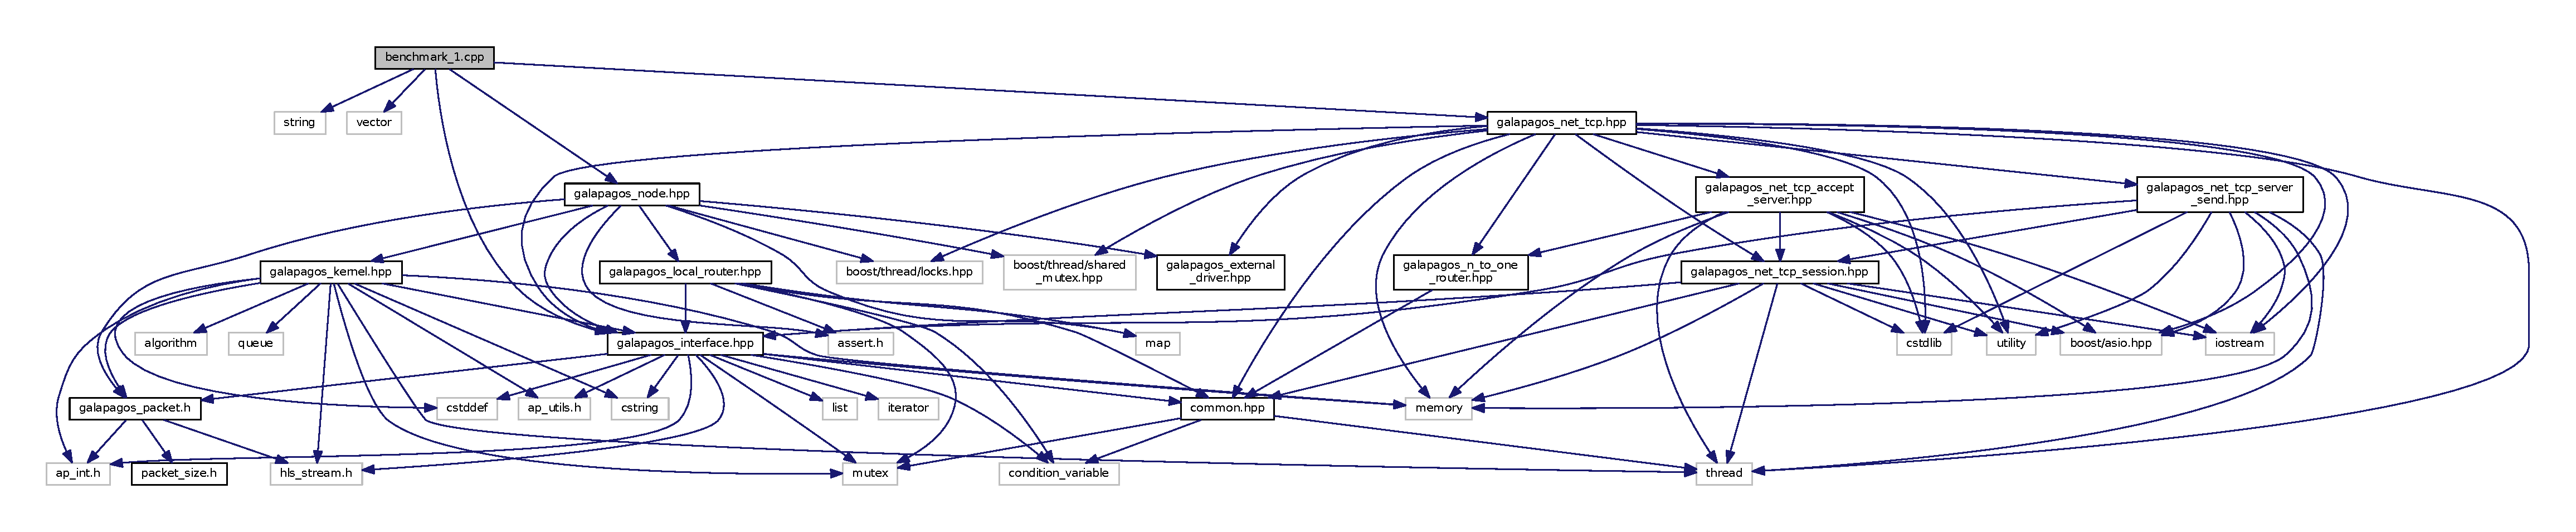
\includegraphics[width=350pt]{benchmark__1_8cpp__incl}
\end{center}
\end{figure}
\subsection*{Macros}
\begin{DoxyCompactItemize}
\item 
\#define \hyperlink{benchmark__1_8cpp_ab3be0641eb76161a48ed528e6eea2ac3}{N\+U\+M\+\_\+\+I\+T\+E\+R\+A\+T\+I\+O\+NS}~100000
\end{DoxyCompactItemize}
\subsection*{Functions}
\begin{DoxyCompactItemize}
\item 
void \hyperlink{benchmark__1_8cpp_a952c103146dc9b79782931ba3fa131f1}{generate\+\_\+flit} (int iterations, int size, int id, int dest, \hyperlink{galapagos__interface_8hpp_af5070d0f7a016a7cd5677cdf2e30ac63}{galapagos\+\_\+interface} $\ast$out)
\item 
auto \hyperlink{benchmark__1_8cpp_afc8eb6b6cadc5c14cdf86a742ee312a9}{start\+\_\+timer} ()
\item 
void \hyperlink{benchmark__1_8cpp_adb55cd51f1bde00069b064101c60d86f}{print\+\_\+time} (std\+::chrono\+::high\+\_\+resolution\+\_\+clock\+::time\+\_\+point timer, std\+::string label)
\item 
void \hyperlink{benchmark__1_8cpp_a54f037e7a8d79a8557a33713c97c3ed8}{generate\+\_\+packet} (int iterations, int size, int id, int dest, \hyperlink{galapagos__interface_8hpp_af5070d0f7a016a7cd5677cdf2e30ac63}{galapagos\+\_\+interface} $\ast$out)
\item 
void \hyperlink{benchmark__1_8cpp_a79daffd29405a76f0c0676b577e2843d}{generate\+\_\+packet} (char $\ast$mem, int iterations, int size, int id, int dest, \hyperlink{galapagos__interface_8hpp_af5070d0f7a016a7cd5677cdf2e30ac63}{galapagos\+\_\+interface} $\ast$out)
\item 
void \hyperlink{benchmark__1_8cpp_a83fe9f71488e293cfe12208b9a4b082a}{generate\+\_\+packet} (std\+::vector$<$ ap\+\_\+uint$<$ 64 $>$ $>$ $\ast$vec, int iterations, int size, int id, int dest, \hyperlink{galapagos__interface_8hpp_af5070d0f7a016a7cd5677cdf2e30ac63}{galapagos\+\_\+interface} $\ast$out)
\item 
void \hyperlink{benchmark__1_8cpp_ab58f1ce436d790a26a5c52969cb832aa}{receive\+\_\+flit\+\_\+perf} (int iterations, int size, \hyperlink{galapagos__interface_8hpp_af5070d0f7a016a7cd5677cdf2e30ac63}{galapagos\+\_\+interface} $\ast$in)
\item 
void \hyperlink{benchmark__1_8cpp_affc065c5706e3d2766ff79d86064eba6}{receive\+\_\+packet\+\_\+perf} (int iterations, int size, \hyperlink{galapagos__interface_8hpp_af5070d0f7a016a7cd5677cdf2e30ac63}{galapagos\+\_\+interface} $\ast$in)
\item 
void \hyperlink{benchmark__1_8cpp_a5d0cd200435e0f644ecd4f7b8acf04fb}{receive\+\_\+packet\+\_\+mem\+\_\+perf} (char $\ast$mem, int iterations, int size, \hyperlink{galapagos__interface_8hpp_af5070d0f7a016a7cd5677cdf2e30ac63}{galapagos\+\_\+interface} $\ast$in)
\item 
void \hyperlink{benchmark__1_8cpp_abe8edb4407293362836700570a97a10b}{print\+\_\+throughput} (std\+::string test\+\_\+name, std\+::string test\+\_\+type, int size)
\item 
void \hyperlink{benchmark__1_8cpp_aec791ee0f05029c542c54c2b12fd4e2e}{print\+\_\+latency} (std\+::string test\+\_\+name, std\+::string test\+\_\+type, int size, std\+::chrono\+::duration$<$ double $>$ diff)
\item 
void \hyperlink{benchmark__1_8cpp_ac975e1131da0fa2a45ac276f0cd0dcb0}{kern\+\_\+benchmark\+\_\+reply\+\_\+1} (short id, \hyperlink{galapagos__interface_8hpp_af5070d0f7a016a7cd5677cdf2e30ac63}{galapagos\+\_\+interface} $\ast$in, \hyperlink{galapagos__interface_8hpp_af5070d0f7a016a7cd5677cdf2e30ac63}{galapagos\+\_\+interface} $\ast$out)
\item 
int \hyperlink{benchmark__1_8cpp_ae66f6b31b5ad750f1fe042a706a4e3d4}{main} ()
\end{DoxyCompactItemize}
\subsection*{Variables}
\begin{DoxyCompactItemize}
\item 
std\+::chrono\+::time\+\_\+point$<$ std\+::chrono\+::high\+\_\+resolution\+\_\+clock $>$ \hyperlink{benchmark__1_8cpp_a46dea58f2d527f376090214bd5c3233d}{start}
\item 
std\+::chrono\+::time\+\_\+point$<$ std\+::chrono\+::high\+\_\+resolution\+\_\+clock $>$ \hyperlink{benchmark__1_8cpp_ace54cb99b52f35f3a98f99e2a75dd5ad}{end}
\item 
int \hyperlink{benchmark__1_8cpp_a242878592db6f7a2c418597075681ef7}{msg\+\_\+num} = 11
\item 
int \hyperlink{benchmark__1_8cpp_aba50ac03860735a8b607b2fcbf57dc60}{msg\+\_\+size} \mbox{[}$\,$\mbox{]} = \{1, 2, 4, 8, 16, 32, 64, 128, 256, 512, \hyperlink{galapagos__interface_8hpp_a1d5dab30b404fab91608086105afc78c}{M\+A\+X\+\_\+\+B\+U\+F\+F\+ER}\}
\item 
int \hyperlink{benchmark__1_8cpp_a9d85b8fff6f70aa502b3c74d38c02ded}{msg\+\_\+reply} = 2
\end{DoxyCompactItemize}


\subsection{Macro Definition Documentation}
\index{benchmark\+\_\+1.\+cpp@{benchmark\+\_\+1.\+cpp}!N\+U\+M\+\_\+\+I\+T\+E\+R\+A\+T\+I\+O\+NS@{N\+U\+M\+\_\+\+I\+T\+E\+R\+A\+T\+I\+O\+NS}}
\index{N\+U\+M\+\_\+\+I\+T\+E\+R\+A\+T\+I\+O\+NS@{N\+U\+M\+\_\+\+I\+T\+E\+R\+A\+T\+I\+O\+NS}!benchmark\+\_\+1.\+cpp@{benchmark\+\_\+1.\+cpp}}
\subsubsection[{\texorpdfstring{N\+U\+M\+\_\+\+I\+T\+E\+R\+A\+T\+I\+O\+NS}{NUM_ITERATIONS}}]{\setlength{\rightskip}{0pt plus 5cm}\#define N\+U\+M\+\_\+\+I\+T\+E\+R\+A\+T\+I\+O\+NS~100000}\hypertarget{benchmark__1_8cpp_ab3be0641eb76161a48ed528e6eea2ac3}{}\label{benchmark__1_8cpp_ab3be0641eb76161a48ed528e6eea2ac3}


\subsection{Function Documentation}
\index{benchmark\+\_\+1.\+cpp@{benchmark\+\_\+1.\+cpp}!generate\+\_\+flit@{generate\+\_\+flit}}
\index{generate\+\_\+flit@{generate\+\_\+flit}!benchmark\+\_\+1.\+cpp@{benchmark\+\_\+1.\+cpp}}
\subsubsection[{\texorpdfstring{generate\+\_\+flit(int iterations, int size, int id, int dest, galapagos\+\_\+interface $\ast$out)}{generate_flit(int iterations, int size, int id, int dest, galapagos_interface *out)}}]{\setlength{\rightskip}{0pt plus 5cm}void generate\+\_\+flit (
\begin{DoxyParamCaption}
\item[{int}]{iterations, }
\item[{int}]{size, }
\item[{int}]{id, }
\item[{int}]{dest, }
\item[{{\bf galapagos\+\_\+interface} $\ast$}]{out}
\end{DoxyParamCaption}
)}\hypertarget{benchmark__1_8cpp_a952c103146dc9b79782931ba3fa131f1}{}\label{benchmark__1_8cpp_a952c103146dc9b79782931ba3fa131f1}
\index{benchmark\+\_\+1.\+cpp@{benchmark\+\_\+1.\+cpp}!generate\+\_\+packet@{generate\+\_\+packet}}
\index{generate\+\_\+packet@{generate\+\_\+packet}!benchmark\+\_\+1.\+cpp@{benchmark\+\_\+1.\+cpp}}
\subsubsection[{\texorpdfstring{generate\+\_\+packet(int iterations, int size, int id, int dest, galapagos\+\_\+interface $\ast$out)}{generate_packet(int iterations, int size, int id, int dest, galapagos_interface *out)}}]{\setlength{\rightskip}{0pt plus 5cm}void generate\+\_\+packet (
\begin{DoxyParamCaption}
\item[{int}]{iterations, }
\item[{int}]{size, }
\item[{int}]{id, }
\item[{int}]{dest, }
\item[{{\bf galapagos\+\_\+interface} $\ast$}]{out}
\end{DoxyParamCaption}
)}\hypertarget{benchmark__1_8cpp_a54f037e7a8d79a8557a33713c97c3ed8}{}\label{benchmark__1_8cpp_a54f037e7a8d79a8557a33713c97c3ed8}
\index{benchmark\+\_\+1.\+cpp@{benchmark\+\_\+1.\+cpp}!generate\+\_\+packet@{generate\+\_\+packet}}
\index{generate\+\_\+packet@{generate\+\_\+packet}!benchmark\+\_\+1.\+cpp@{benchmark\+\_\+1.\+cpp}}
\subsubsection[{\texorpdfstring{generate\+\_\+packet(char $\ast$mem, int iterations, int size, int id, int dest, galapagos\+\_\+interface $\ast$out)}{generate_packet(char *mem, int iterations, int size, int id, int dest, galapagos_interface *out)}}]{\setlength{\rightskip}{0pt plus 5cm}void generate\+\_\+packet (
\begin{DoxyParamCaption}
\item[{char $\ast$}]{mem, }
\item[{int}]{iterations, }
\item[{int}]{size, }
\item[{int}]{id, }
\item[{int}]{dest, }
\item[{{\bf galapagos\+\_\+interface} $\ast$}]{out}
\end{DoxyParamCaption}
)}\hypertarget{benchmark__1_8cpp_a79daffd29405a76f0c0676b577e2843d}{}\label{benchmark__1_8cpp_a79daffd29405a76f0c0676b577e2843d}
\index{benchmark\+\_\+1.\+cpp@{benchmark\+\_\+1.\+cpp}!generate\+\_\+packet@{generate\+\_\+packet}}
\index{generate\+\_\+packet@{generate\+\_\+packet}!benchmark\+\_\+1.\+cpp@{benchmark\+\_\+1.\+cpp}}
\subsubsection[{\texorpdfstring{generate\+\_\+packet(std\+::vector$<$ ap\+\_\+uint$<$ 64 $>$ $>$ $\ast$vec, int iterations, int size, int id, int dest, galapagos\+\_\+interface $\ast$out)}{generate_packet(std::vector< ap_uint< 64 > > *vec, int iterations, int size, int id, int dest, galapagos_interface *out)}}]{\setlength{\rightskip}{0pt plus 5cm}void generate\+\_\+packet (
\begin{DoxyParamCaption}
\item[{std\+::vector$<$ ap\+\_\+uint$<$ 64 $>$ $>$ $\ast$}]{vec, }
\item[{int}]{iterations, }
\item[{int}]{size, }
\item[{int}]{id, }
\item[{int}]{dest, }
\item[{{\bf galapagos\+\_\+interface} $\ast$}]{out}
\end{DoxyParamCaption}
)}\hypertarget{benchmark__1_8cpp_a83fe9f71488e293cfe12208b9a4b082a}{}\label{benchmark__1_8cpp_a83fe9f71488e293cfe12208b9a4b082a}
\index{benchmark\+\_\+1.\+cpp@{benchmark\+\_\+1.\+cpp}!kern\+\_\+benchmark\+\_\+reply\+\_\+1@{kern\+\_\+benchmark\+\_\+reply\+\_\+1}}
\index{kern\+\_\+benchmark\+\_\+reply\+\_\+1@{kern\+\_\+benchmark\+\_\+reply\+\_\+1}!benchmark\+\_\+1.\+cpp@{benchmark\+\_\+1.\+cpp}}
\subsubsection[{\texorpdfstring{kern\+\_\+benchmark\+\_\+reply\+\_\+1(short id, galapagos\+\_\+interface $\ast$in, galapagos\+\_\+interface $\ast$out)}{kern_benchmark_reply_1(short id, galapagos_interface *in, galapagos_interface *out)}}]{\setlength{\rightskip}{0pt plus 5cm}void kern\+\_\+benchmark\+\_\+reply\+\_\+1 (
\begin{DoxyParamCaption}
\item[{short}]{id, }
\item[{{\bf galapagos\+\_\+interface} $\ast$}]{in, }
\item[{{\bf galapagos\+\_\+interface} $\ast$}]{out}
\end{DoxyParamCaption}
)}\hypertarget{benchmark__1_8cpp_ac975e1131da0fa2a45ac276f0cd0dcb0}{}\label{benchmark__1_8cpp_ac975e1131da0fa2a45ac276f0cd0dcb0}
\index{benchmark\+\_\+1.\+cpp@{benchmark\+\_\+1.\+cpp}!main@{main}}
\index{main@{main}!benchmark\+\_\+1.\+cpp@{benchmark\+\_\+1.\+cpp}}
\subsubsection[{\texorpdfstring{main()}{main()}}]{\setlength{\rightskip}{0pt plus 5cm}int main (
\begin{DoxyParamCaption}
{}
\end{DoxyParamCaption}
)}\hypertarget{benchmark__1_8cpp_ae66f6b31b5ad750f1fe042a706a4e3d4}{}\label{benchmark__1_8cpp_ae66f6b31b5ad750f1fe042a706a4e3d4}
\index{benchmark\+\_\+1.\+cpp@{benchmark\+\_\+1.\+cpp}!print\+\_\+latency@{print\+\_\+latency}}
\index{print\+\_\+latency@{print\+\_\+latency}!benchmark\+\_\+1.\+cpp@{benchmark\+\_\+1.\+cpp}}
\subsubsection[{\texorpdfstring{print\+\_\+latency(std\+::string test\+\_\+name, std\+::string test\+\_\+type, int size, std\+::chrono\+::duration$<$ double $>$ diff)}{print_latency(std::string test_name, std::string test_type, int size, std::chrono::duration< double > diff)}}]{\setlength{\rightskip}{0pt plus 5cm}void print\+\_\+latency (
\begin{DoxyParamCaption}
\item[{std\+::string}]{test\+\_\+name, }
\item[{std\+::string}]{test\+\_\+type, }
\item[{int}]{size, }
\item[{std\+::chrono\+::duration$<$ double $>$}]{diff}
\end{DoxyParamCaption}
)}\hypertarget{benchmark__1_8cpp_aec791ee0f05029c542c54c2b12fd4e2e}{}\label{benchmark__1_8cpp_aec791ee0f05029c542c54c2b12fd4e2e}
\index{benchmark\+\_\+1.\+cpp@{benchmark\+\_\+1.\+cpp}!print\+\_\+throughput@{print\+\_\+throughput}}
\index{print\+\_\+throughput@{print\+\_\+throughput}!benchmark\+\_\+1.\+cpp@{benchmark\+\_\+1.\+cpp}}
\subsubsection[{\texorpdfstring{print\+\_\+throughput(std\+::string test\+\_\+name, std\+::string test\+\_\+type, int size)}{print_throughput(std::string test_name, std::string test_type, int size)}}]{\setlength{\rightskip}{0pt plus 5cm}void print\+\_\+throughput (
\begin{DoxyParamCaption}
\item[{std\+::string}]{test\+\_\+name, }
\item[{std\+::string}]{test\+\_\+type, }
\item[{int}]{size}
\end{DoxyParamCaption}
)}\hypertarget{benchmark__1_8cpp_abe8edb4407293362836700570a97a10b}{}\label{benchmark__1_8cpp_abe8edb4407293362836700570a97a10b}
\index{benchmark\+\_\+1.\+cpp@{benchmark\+\_\+1.\+cpp}!print\+\_\+time@{print\+\_\+time}}
\index{print\+\_\+time@{print\+\_\+time}!benchmark\+\_\+1.\+cpp@{benchmark\+\_\+1.\+cpp}}
\subsubsection[{\texorpdfstring{print\+\_\+time(std\+::chrono\+::high\+\_\+resolution\+\_\+clock\+::time\+\_\+point timer, std\+::string label)}{print_time(std::chrono::high_resolution_clock::time_point timer, std::string label)}}]{\setlength{\rightskip}{0pt plus 5cm}void print\+\_\+time (
\begin{DoxyParamCaption}
\item[{std\+::chrono\+::high\+\_\+resolution\+\_\+clock\+::time\+\_\+point}]{timer, }
\item[{std\+::string}]{label}
\end{DoxyParamCaption}
)}\hypertarget{benchmark__1_8cpp_adb55cd51f1bde00069b064101c60d86f}{}\label{benchmark__1_8cpp_adb55cd51f1bde00069b064101c60d86f}
\index{benchmark\+\_\+1.\+cpp@{benchmark\+\_\+1.\+cpp}!receive\+\_\+flit\+\_\+perf@{receive\+\_\+flit\+\_\+perf}}
\index{receive\+\_\+flit\+\_\+perf@{receive\+\_\+flit\+\_\+perf}!benchmark\+\_\+1.\+cpp@{benchmark\+\_\+1.\+cpp}}
\subsubsection[{\texorpdfstring{receive\+\_\+flit\+\_\+perf(int iterations, int size, galapagos\+\_\+interface $\ast$in)}{receive_flit_perf(int iterations, int size, galapagos_interface *in)}}]{\setlength{\rightskip}{0pt plus 5cm}void receive\+\_\+flit\+\_\+perf (
\begin{DoxyParamCaption}
\item[{int}]{iterations, }
\item[{int}]{size, }
\item[{{\bf galapagos\+\_\+interface} $\ast$}]{in}
\end{DoxyParamCaption}
)}\hypertarget{benchmark__1_8cpp_ab58f1ce436d790a26a5c52969cb832aa}{}\label{benchmark__1_8cpp_ab58f1ce436d790a26a5c52969cb832aa}
\index{benchmark\+\_\+1.\+cpp@{benchmark\+\_\+1.\+cpp}!receive\+\_\+packet\+\_\+mem\+\_\+perf@{receive\+\_\+packet\+\_\+mem\+\_\+perf}}
\index{receive\+\_\+packet\+\_\+mem\+\_\+perf@{receive\+\_\+packet\+\_\+mem\+\_\+perf}!benchmark\+\_\+1.\+cpp@{benchmark\+\_\+1.\+cpp}}
\subsubsection[{\texorpdfstring{receive\+\_\+packet\+\_\+mem\+\_\+perf(char $\ast$mem, int iterations, int size, galapagos\+\_\+interface $\ast$in)}{receive_packet_mem_perf(char *mem, int iterations, int size, galapagos_interface *in)}}]{\setlength{\rightskip}{0pt plus 5cm}void receive\+\_\+packet\+\_\+mem\+\_\+perf (
\begin{DoxyParamCaption}
\item[{char $\ast$}]{mem, }
\item[{int}]{iterations, }
\item[{int}]{size, }
\item[{{\bf galapagos\+\_\+interface} $\ast$}]{in}
\end{DoxyParamCaption}
)}\hypertarget{benchmark__1_8cpp_a5d0cd200435e0f644ecd4f7b8acf04fb}{}\label{benchmark__1_8cpp_a5d0cd200435e0f644ecd4f7b8acf04fb}
\index{benchmark\+\_\+1.\+cpp@{benchmark\+\_\+1.\+cpp}!receive\+\_\+packet\+\_\+perf@{receive\+\_\+packet\+\_\+perf}}
\index{receive\+\_\+packet\+\_\+perf@{receive\+\_\+packet\+\_\+perf}!benchmark\+\_\+1.\+cpp@{benchmark\+\_\+1.\+cpp}}
\subsubsection[{\texorpdfstring{receive\+\_\+packet\+\_\+perf(int iterations, int size, galapagos\+\_\+interface $\ast$in)}{receive_packet_perf(int iterations, int size, galapagos_interface *in)}}]{\setlength{\rightskip}{0pt plus 5cm}void receive\+\_\+packet\+\_\+perf (
\begin{DoxyParamCaption}
\item[{int}]{iterations, }
\item[{int}]{size, }
\item[{{\bf galapagos\+\_\+interface} $\ast$}]{in}
\end{DoxyParamCaption}
)}\hypertarget{benchmark__1_8cpp_affc065c5706e3d2766ff79d86064eba6}{}\label{benchmark__1_8cpp_affc065c5706e3d2766ff79d86064eba6}
\index{benchmark\+\_\+1.\+cpp@{benchmark\+\_\+1.\+cpp}!start\+\_\+timer@{start\+\_\+timer}}
\index{start\+\_\+timer@{start\+\_\+timer}!benchmark\+\_\+1.\+cpp@{benchmark\+\_\+1.\+cpp}}
\subsubsection[{\texorpdfstring{start\+\_\+timer()}{start_timer()}}]{\setlength{\rightskip}{0pt plus 5cm}auto start\+\_\+timer (
\begin{DoxyParamCaption}
{}
\end{DoxyParamCaption}
)}\hypertarget{benchmark__1_8cpp_afc8eb6b6cadc5c14cdf86a742ee312a9}{}\label{benchmark__1_8cpp_afc8eb6b6cadc5c14cdf86a742ee312a9}


\subsection{Variable Documentation}
\index{benchmark\+\_\+1.\+cpp@{benchmark\+\_\+1.\+cpp}!end@{end}}
\index{end@{end}!benchmark\+\_\+1.\+cpp@{benchmark\+\_\+1.\+cpp}}
\subsubsection[{\texorpdfstring{end}{end}}]{\setlength{\rightskip}{0pt plus 5cm}std\+::chrono\+::time\+\_\+point$<$std\+::chrono\+::high\+\_\+resolution\+\_\+clock$>$ end}\hypertarget{benchmark__1_8cpp_ace54cb99b52f35f3a98f99e2a75dd5ad}{}\label{benchmark__1_8cpp_ace54cb99b52f35f3a98f99e2a75dd5ad}
\index{benchmark\+\_\+1.\+cpp@{benchmark\+\_\+1.\+cpp}!msg\+\_\+num@{msg\+\_\+num}}
\index{msg\+\_\+num@{msg\+\_\+num}!benchmark\+\_\+1.\+cpp@{benchmark\+\_\+1.\+cpp}}
\subsubsection[{\texorpdfstring{msg\+\_\+num}{msg_num}}]{\setlength{\rightskip}{0pt plus 5cm}int msg\+\_\+num = 11}\hypertarget{benchmark__1_8cpp_a242878592db6f7a2c418597075681ef7}{}\label{benchmark__1_8cpp_a242878592db6f7a2c418597075681ef7}
\index{benchmark\+\_\+1.\+cpp@{benchmark\+\_\+1.\+cpp}!msg\+\_\+reply@{msg\+\_\+reply}}
\index{msg\+\_\+reply@{msg\+\_\+reply}!benchmark\+\_\+1.\+cpp@{benchmark\+\_\+1.\+cpp}}
\subsubsection[{\texorpdfstring{msg\+\_\+reply}{msg_reply}}]{\setlength{\rightskip}{0pt plus 5cm}int msg\+\_\+reply = 2}\hypertarget{benchmark__1_8cpp_a9d85b8fff6f70aa502b3c74d38c02ded}{}\label{benchmark__1_8cpp_a9d85b8fff6f70aa502b3c74d38c02ded}
\index{benchmark\+\_\+1.\+cpp@{benchmark\+\_\+1.\+cpp}!msg\+\_\+size@{msg\+\_\+size}}
\index{msg\+\_\+size@{msg\+\_\+size}!benchmark\+\_\+1.\+cpp@{benchmark\+\_\+1.\+cpp}}
\subsubsection[{\texorpdfstring{msg\+\_\+size}{msg_size}}]{\setlength{\rightskip}{0pt plus 5cm}int msg\+\_\+size\mbox{[}$\,$\mbox{]} = \{1, 2, 4, 8, 16, 32, 64, 128, 256, 512, {\bf M\+A\+X\+\_\+\+B\+U\+F\+F\+ER}\}}\hypertarget{benchmark__1_8cpp_aba50ac03860735a8b607b2fcbf57dc60}{}\label{benchmark__1_8cpp_aba50ac03860735a8b607b2fcbf57dc60}
\index{benchmark\+\_\+1.\+cpp@{benchmark\+\_\+1.\+cpp}!start@{start}}
\index{start@{start}!benchmark\+\_\+1.\+cpp@{benchmark\+\_\+1.\+cpp}}
\subsubsection[{\texorpdfstring{start}{start}}]{\setlength{\rightskip}{0pt plus 5cm}std\+::chrono\+::time\+\_\+point$<$std\+::chrono\+::high\+\_\+resolution\+\_\+clock$>$ start}\hypertarget{benchmark__1_8cpp_a46dea58f2d527f376090214bd5c3233d}{}\label{benchmark__1_8cpp_a46dea58f2d527f376090214bd5c3233d}

\hypertarget{common_8cpp}{}\section{common.\+cpp File Reference}
\label{common_8cpp}\index{common.\+cpp@{common.\+cpp}}
{\ttfamily \#include \char`\"{}common.\+hpp\char`\"{}}\\*
{\ttfamily \#include \char`\"{}math.\+h\char`\"{}}\\*
Include dependency graph for common.\+cpp\+:
\nopagebreak
\begin{figure}[H]
\begin{center}
\leavevmode
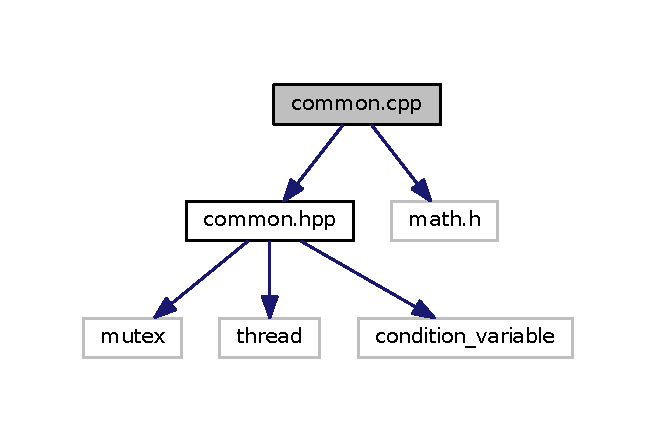
\includegraphics[width=315pt]{common_8cpp__incl}
\end{center}
\end{figure}

\hypertarget{common_8hpp}{}\section{common.\+hpp File Reference}
\label{common_8hpp}\index{common.\+hpp@{common.\+hpp}}
{\ttfamily \#include $<$mutex$>$}\\*
{\ttfamily \#include $<$thread$>$}\\*
{\ttfamily \#include $<$condition\+\_\+variable$>$}\\*
Include dependency graph for common.\+hpp\+:
\nopagebreak
\begin{figure}[H]
\begin{center}
\leavevmode
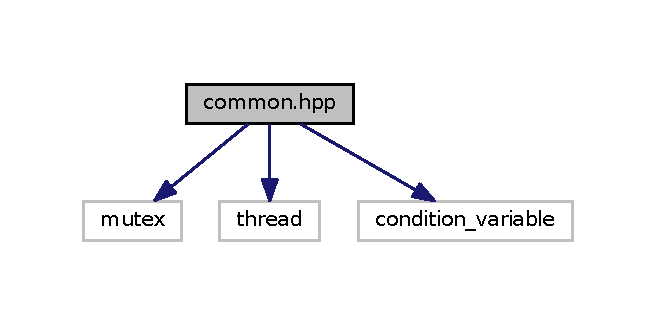
\includegraphics[width=315pt]{common_8hpp__incl}
\end{center}
\end{figure}
This graph shows which files directly or indirectly include this file\+:
\nopagebreak
\begin{figure}[H]
\begin{center}
\leavevmode
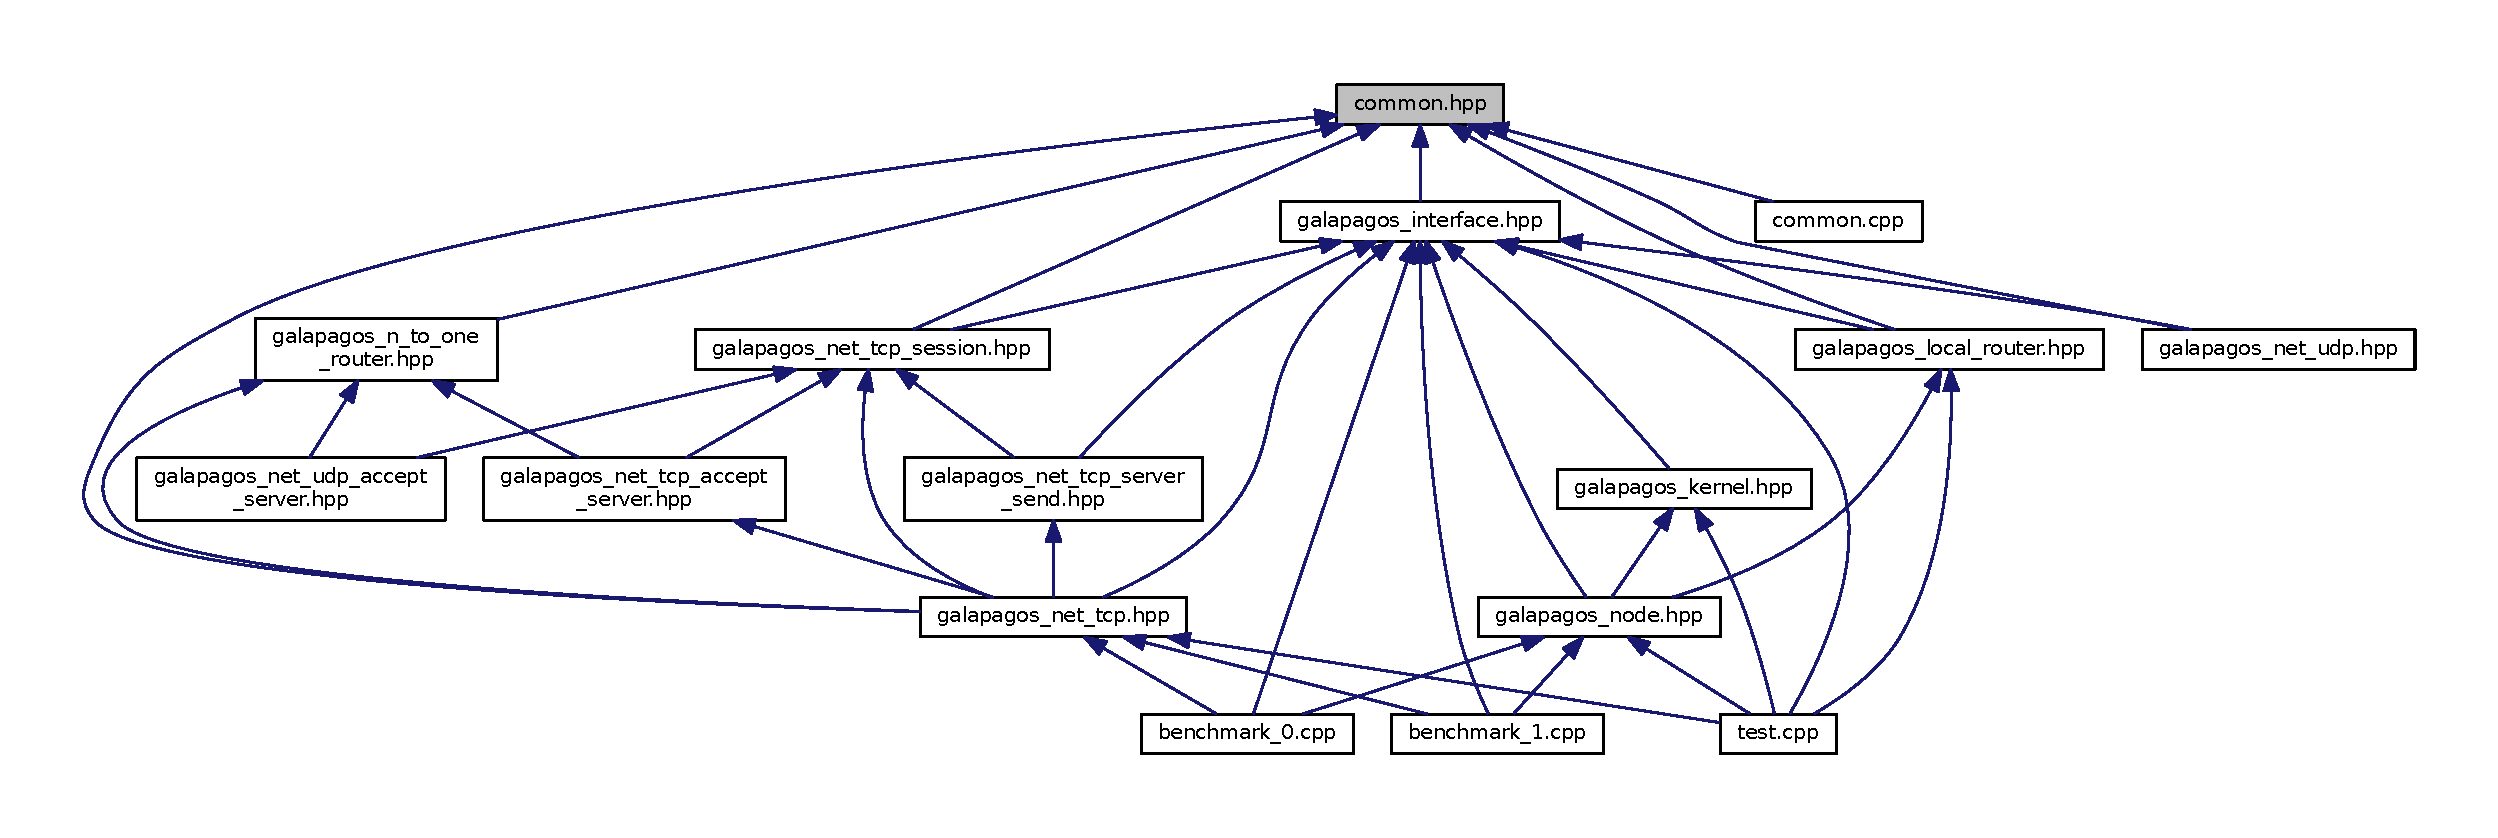
\includegraphics[width=350pt]{common_8hpp__dep__incl}
\end{center}
\end{figure}
\subsection*{Classes}
\begin{DoxyCompactItemize}
\item 
struct \hyperlink{structgalapagos_1_1__done__struct}{galapagos\+::\+\_\+done\+\_\+struct}
\item 
struct \hyperlink{structgalapagos_1_1__num__threadsafe}{galapagos\+::\+\_\+num\+\_\+threadsafe}
\item 
class \hyperlink{classgalapagos_1_1done__clean}{galapagos\+::done\+\_\+clean}
\end{DoxyCompactItemize}
\subsection*{Namespaces}
\begin{DoxyCompactItemize}
\item 
 \hyperlink{namespacegalapagos}{galapagos}
\end{DoxyCompactItemize}
\subsection*{Macros}
\begin{DoxyCompactItemize}
\item 
\#define \hyperlink{common_8hpp_a5f857c49d70f30382a1ce70dbf5ebccc}{P\+O\+W\+E\+R\+\_\+2}(x)~(1\+U\+L\+L $<$$<$ (x))
\end{DoxyCompactItemize}
\subsection*{Functions}
\begin{DoxyCompactItemize}
\item 
{\footnotesize template$<$class T $>$ }\\\hyperlink{test_8cpp_a0658ceffa730c765d449bb3d21871b5f}{T} \hyperlink{namespacegalapagos_a7b825b7d39b5187a8f617fbdd414c747}{galapagos\+::range} (short msb, short lsb, \hyperlink{test_8cpp_a0658ceffa730c765d449bb3d21871b5f}{T} source, size\+\_\+t value)
\item 
{\footnotesize template$<$class T $>$ }\\\hyperlink{test_8cpp_a0658ceffa730c765d449bb3d21871b5f}{T} \hyperlink{namespacegalapagos_adf747977be6d582c3a8b1c38b531c06d}{galapagos\+::range} (short msb, short lsb, \hyperlink{test_8cpp_a0658ceffa730c765d449bb3d21871b5f}{T} source)
\end{DoxyCompactItemize}


\subsection{Macro Definition Documentation}
\index{common.\+hpp@{common.\+hpp}!P\+O\+W\+E\+R\+\_\+2@{P\+O\+W\+E\+R\+\_\+2}}
\index{P\+O\+W\+E\+R\+\_\+2@{P\+O\+W\+E\+R\+\_\+2}!common.\+hpp@{common.\+hpp}}
\subsubsection[{\texorpdfstring{P\+O\+W\+E\+R\+\_\+2}{POWER_2}}]{\setlength{\rightskip}{0pt plus 5cm}\#define P\+O\+W\+E\+R\+\_\+2(
\begin{DoxyParamCaption}
\item[{}]{x}
\end{DoxyParamCaption}
)~(1\+U\+L\+L $<$$<$ (x))}\hypertarget{common_8hpp_a5f857c49d70f30382a1ce70dbf5ebccc}{}\label{common_8hpp_a5f857c49d70f30382a1ce70dbf5ebccc}

\hypertarget{galapagos__external__driver_8hpp}{}\section{galapagos\+\_\+external\+\_\+driver.\+hpp File Reference}
\label{galapagos__external__driver_8hpp}\index{galapagos\+\_\+external\+\_\+driver.\+hpp@{galapagos\+\_\+external\+\_\+driver.\+hpp}}
This graph shows which files directly or indirectly include this file\+:
\nopagebreak
\begin{figure}[H]
\begin{center}
\leavevmode
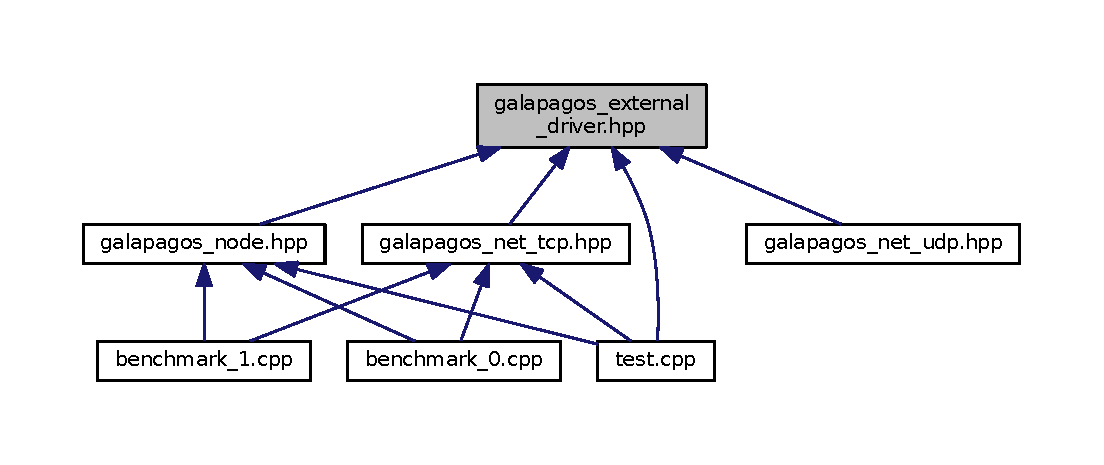
\includegraphics[width=350pt]{galapagos__external__driver_8hpp__dep__incl}
\end{center}
\end{figure}
\subsection*{Classes}
\begin{DoxyCompactItemize}
\item 
class \hyperlink{classgalapagos_1_1external__driver}{galapagos\+::external\+\_\+driver$<$ T $>$}
\end{DoxyCompactItemize}
\subsection*{Namespaces}
\begin{DoxyCompactItemize}
\item 
 \hyperlink{namespacegalapagos}{galapagos}
\end{DoxyCompactItemize}

\hypertarget{galapagos__interface_8hpp}{}\section{galapagos\+\_\+interface.\+hpp File Reference}
\label{galapagos__interface_8hpp}\index{galapagos\+\_\+interface.\+hpp@{galapagos\+\_\+interface.\+hpp}}
{\ttfamily \#include $<$cstddef$>$}\\*
{\ttfamily \#include $<$cstring$>$}\\*
{\ttfamily \#include \char`\"{}ap\+\_\+int.\+h\char`\"{}}\\*
{\ttfamily \#include \char`\"{}hls\+\_\+stream.\+h\char`\"{}}\\*
{\ttfamily \#include \char`\"{}ap\+\_\+utils.\+h\char`\"{}}\\*
{\ttfamily \#include $<$memory$>$}\\*
{\ttfamily \#include $<$mutex$>$}\\*
{\ttfamily \#include $<$condition\+\_\+variable$>$}\\*
{\ttfamily \#include $<$list$>$}\\*
{\ttfamily \#include $<$iterator$>$}\\*
{\ttfamily \#include \char`\"{}common.\+hpp\char`\"{}}\\*
{\ttfamily \#include \char`\"{}galapagos\+\_\+packet.\+h\char`\"{}}\\*
Include dependency graph for galapagos\+\_\+interface.\+hpp\+:
\nopagebreak
\begin{figure}[H]
\begin{center}
\leavevmode
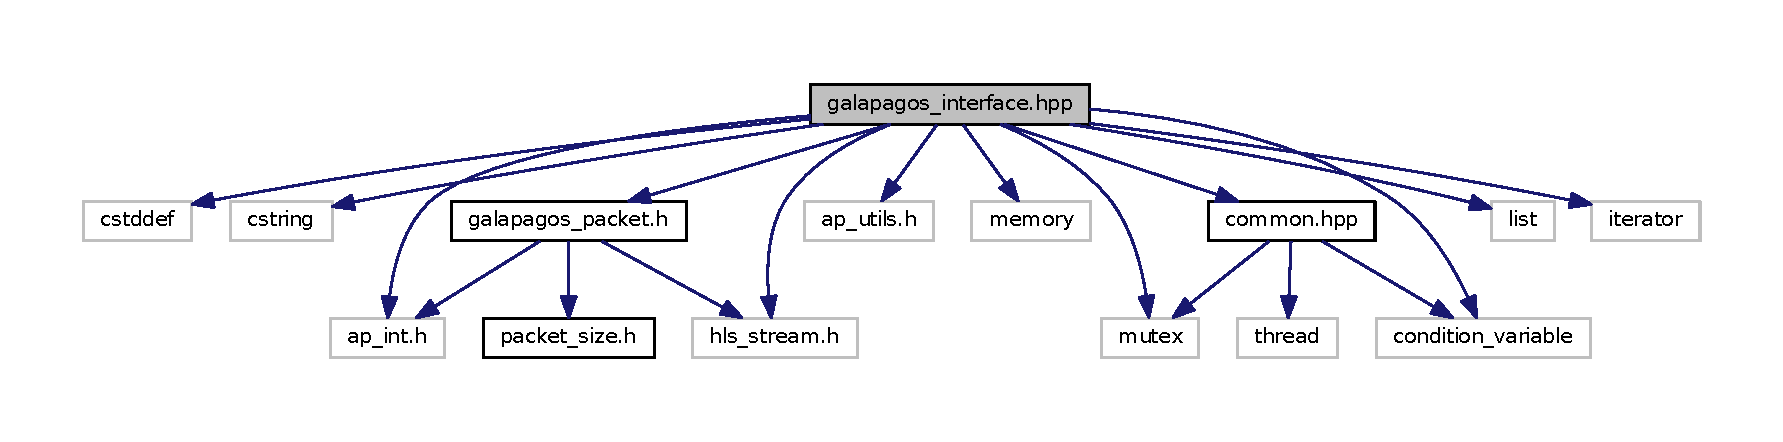
\includegraphics[width=350pt]{galapagos__interface_8hpp__incl}
\end{center}
\end{figure}
This graph shows which files directly or indirectly include this file\+:
\nopagebreak
\begin{figure}[H]
\begin{center}
\leavevmode
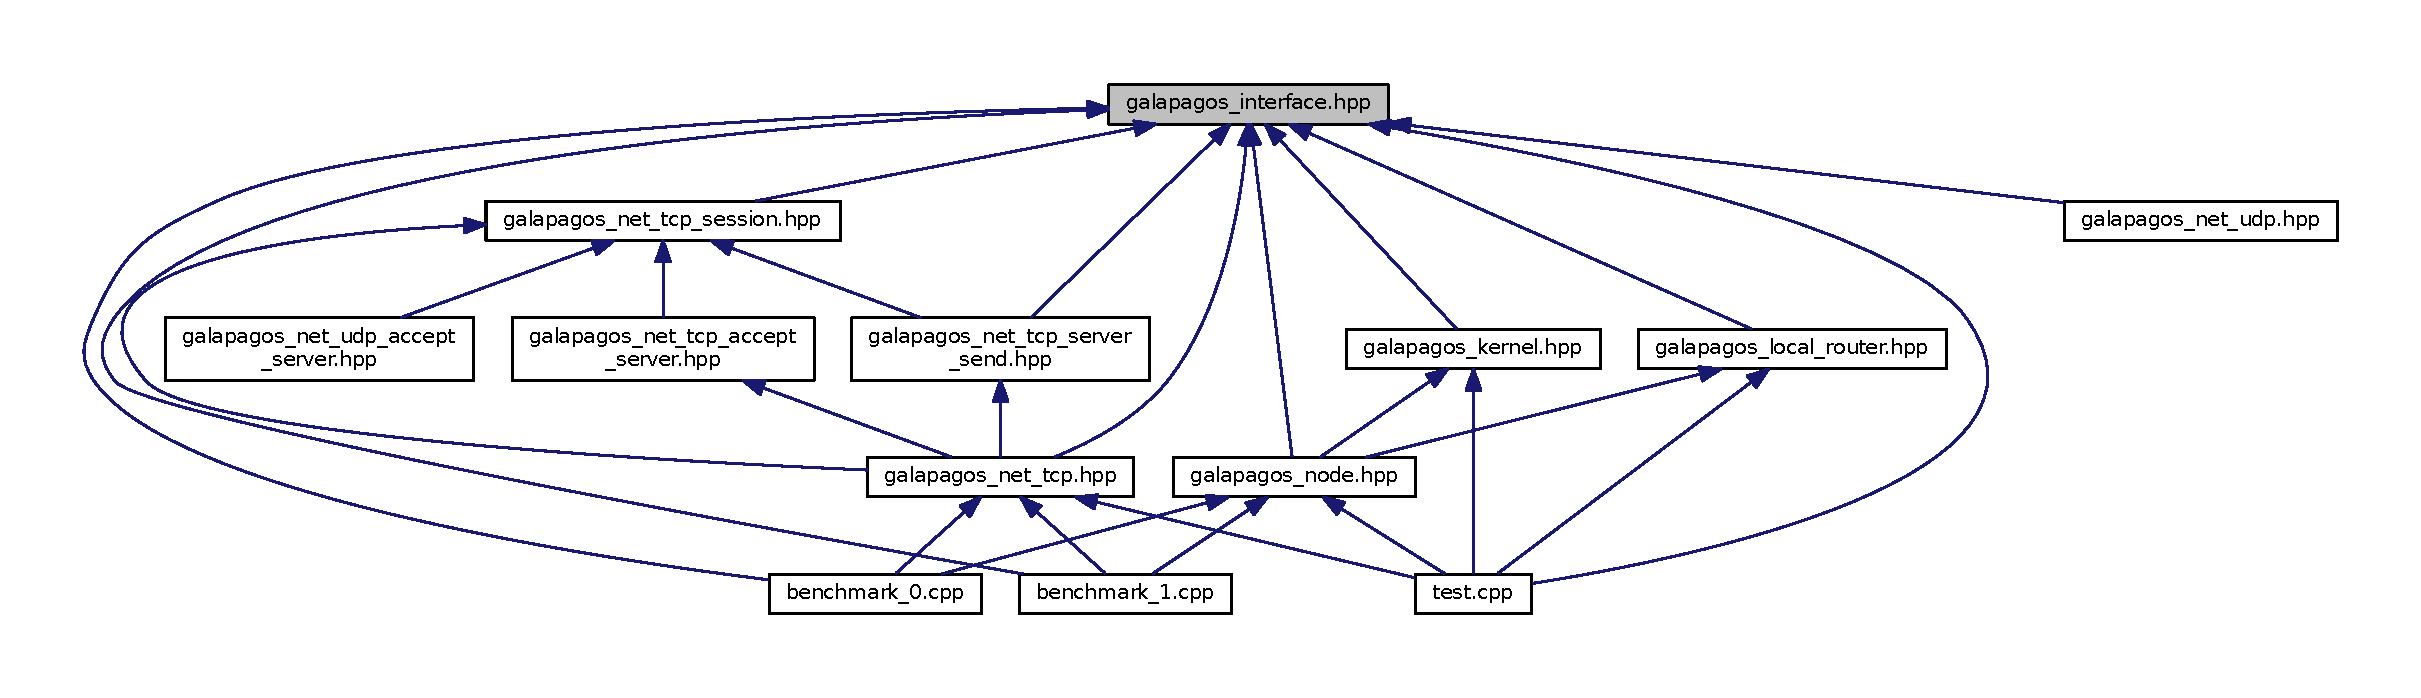
\includegraphics[width=350pt]{galapagos__interface_8hpp__dep__incl}
\end{center}
\end{figure}
\subsection*{Classes}
\begin{DoxyCompactItemize}
\item 
struct \hyperlink{structgalapagos_1_1buffer}{galapagos\+::buffer}
\item 
class \hyperlink{classgalapagos_1_1interface}{galapagos\+::interface$<$ T $>$}
\begin{DoxyCompactList}\small\item\em Class for the Galapagos Interface. \end{DoxyCompactList}\end{DoxyCompactItemize}
\subsection*{Namespaces}
\begin{DoxyCompactItemize}
\item 
 \hyperlink{namespacegalapagos}{galapagos}
\end{DoxyCompactItemize}
\subsection*{Macros}
\begin{DoxyCompactItemize}
\item 
\#define \hyperlink{galapagos__interface_8hpp_a61d2efd85d3ecd2ff366551d189d8677}{J\+U\+M\+B\+O\+\_\+\+F\+R\+A\+ME}
\item 
\#define \hyperlink{galapagos__interface_8hpp_a1d5dab30b404fab91608086105afc78c}{M\+A\+X\+\_\+\+B\+U\+F\+F\+ER}~1124
\end{DoxyCompactItemize}
\subsection*{Typedefs}
\begin{DoxyCompactItemize}
\item 
typedef \hyperlink{classgalapagos_1_1interface}{galapagos\+::interface}$<$ ap\+\_\+uint$<$ \hyperlink{packet__size_8h_aaf115bf32d6740657027593bc293743c}{P\+A\+C\+K\+E\+T\+\_\+\+D\+A\+T\+A\+\_\+\+L\+E\+N\+G\+TH} $>$ $>$ \hyperlink{galapagos__interface_8hpp_af5070d0f7a016a7cd5677cdf2e30ac63}{galapagos\+\_\+interface}
\end{DoxyCompactItemize}


\subsection{Macro Definition Documentation}
\index{galapagos\+\_\+interface.\+hpp@{galapagos\+\_\+interface.\+hpp}!J\+U\+M\+B\+O\+\_\+\+F\+R\+A\+ME@{J\+U\+M\+B\+O\+\_\+\+F\+R\+A\+ME}}
\index{J\+U\+M\+B\+O\+\_\+\+F\+R\+A\+ME@{J\+U\+M\+B\+O\+\_\+\+F\+R\+A\+ME}!galapagos\+\_\+interface.\+hpp@{galapagos\+\_\+interface.\+hpp}}
\subsubsection[{\texorpdfstring{J\+U\+M\+B\+O\+\_\+\+F\+R\+A\+ME}{JUMBO_FRAME}}]{\setlength{\rightskip}{0pt plus 5cm}\#define J\+U\+M\+B\+O\+\_\+\+F\+R\+A\+ME}\hypertarget{galapagos__interface_8hpp_a61d2efd85d3ecd2ff366551d189d8677}{}\label{galapagos__interface_8hpp_a61d2efd85d3ecd2ff366551d189d8677}
\index{galapagos\+\_\+interface.\+hpp@{galapagos\+\_\+interface.\+hpp}!M\+A\+X\+\_\+\+B\+U\+F\+F\+ER@{M\+A\+X\+\_\+\+B\+U\+F\+F\+ER}}
\index{M\+A\+X\+\_\+\+B\+U\+F\+F\+ER@{M\+A\+X\+\_\+\+B\+U\+F\+F\+ER}!galapagos\+\_\+interface.\+hpp@{galapagos\+\_\+interface.\+hpp}}
\subsubsection[{\texorpdfstring{M\+A\+X\+\_\+\+B\+U\+F\+F\+ER}{MAX_BUFFER}}]{\setlength{\rightskip}{0pt plus 5cm}\#define M\+A\+X\+\_\+\+B\+U\+F\+F\+ER~1124}\hypertarget{galapagos__interface_8hpp_a1d5dab30b404fab91608086105afc78c}{}\label{galapagos__interface_8hpp_a1d5dab30b404fab91608086105afc78c}


\subsection{Typedef Documentation}
\index{galapagos\+\_\+interface.\+hpp@{galapagos\+\_\+interface.\+hpp}!galapagos\+\_\+interface@{galapagos\+\_\+interface}}
\index{galapagos\+\_\+interface@{galapagos\+\_\+interface}!galapagos\+\_\+interface.\+hpp@{galapagos\+\_\+interface.\+hpp}}
\subsubsection[{\texorpdfstring{galapagos\+\_\+interface}{galapagos_interface}}]{\setlength{\rightskip}{0pt plus 5cm}typedef {\bf galapagos\+::interface}$<$ap\+\_\+uint$<${\bf P\+A\+C\+K\+E\+T\+\_\+\+D\+A\+T\+A\+\_\+\+L\+E\+N\+G\+TH}$>$ $>$ {\bf galapagos\+\_\+interface}}\hypertarget{galapagos__interface_8hpp_af5070d0f7a016a7cd5677cdf2e30ac63}{}\label{galapagos__interface_8hpp_af5070d0f7a016a7cd5677cdf2e30ac63}

\hypertarget{galapagos__kernel_8hpp}{}\section{galapagos\+\_\+kernel.\+hpp File Reference}
\label{galapagos__kernel_8hpp}\index{galapagos\+\_\+kernel.\+hpp@{galapagos\+\_\+kernel.\+hpp}}
{\ttfamily \#include $<$cstddef$>$}\\*
{\ttfamily \#include $<$cstring$>$}\\*
{\ttfamily \#include \char`\"{}ap\+\_\+int.\+h\char`\"{}}\\*
{\ttfamily \#include \char`\"{}hls\+\_\+stream.\+h\char`\"{}}\\*
{\ttfamily \#include \char`\"{}ap\+\_\+utils.\+h\char`\"{}}\\*
{\ttfamily \#include $<$algorithm$>$}\\*
{\ttfamily \#include $<$memory$>$}\\*
{\ttfamily \#include $<$thread$>$}\\*
{\ttfamily \#include $<$queue$>$}\\*
{\ttfamily \#include $<$mutex$>$}\\*
{\ttfamily \#include \char`\"{}galapagos\+\_\+interface.\+hpp\char`\"{}}\\*
{\ttfamily \#include \char`\"{}galapagos\+\_\+packet.\+h\char`\"{}}\\*
Include dependency graph for galapagos\+\_\+kernel.\+hpp\+:
\nopagebreak
\begin{figure}[H]
\begin{center}
\leavevmode
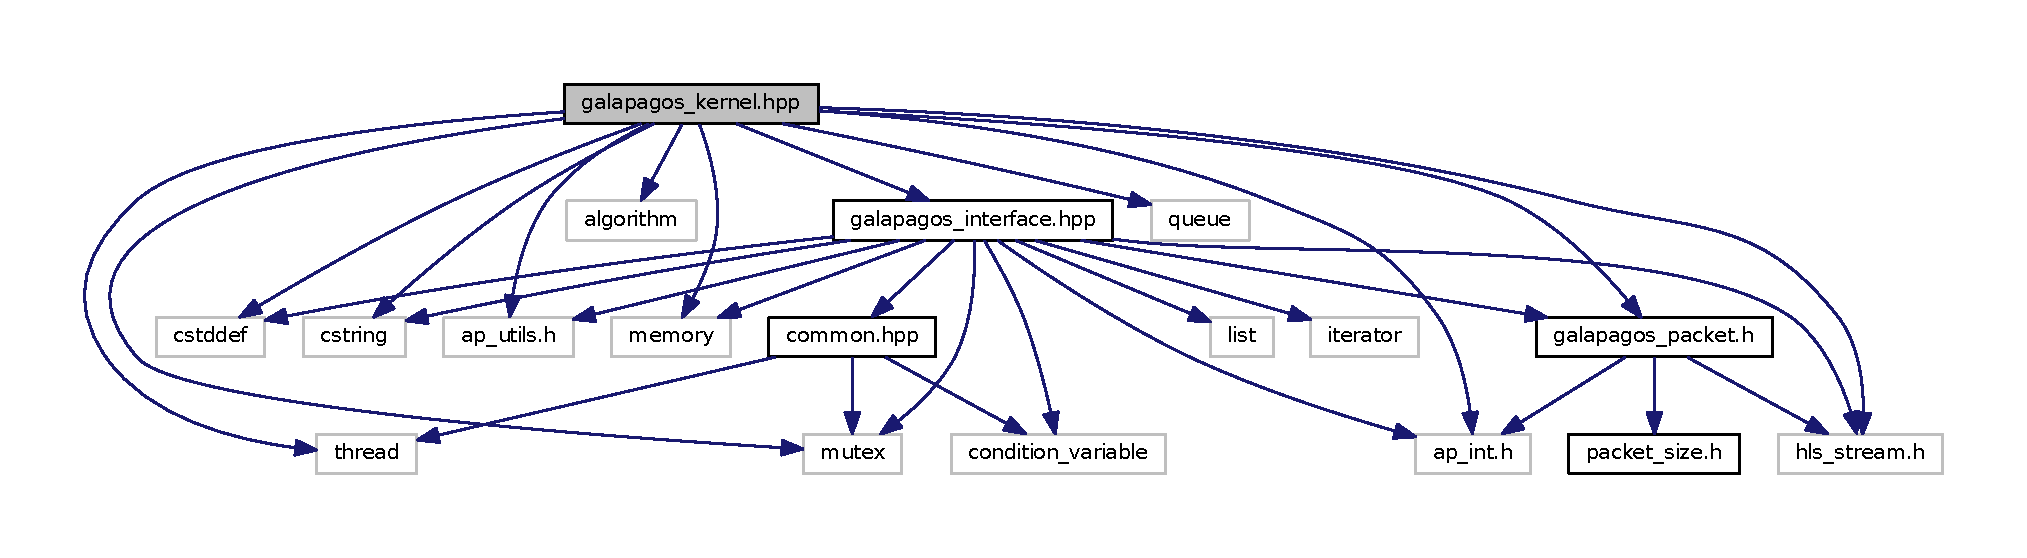
\includegraphics[width=350pt]{galapagos__kernel_8hpp__incl}
\end{center}
\end{figure}
This graph shows which files directly or indirectly include this file\+:
\nopagebreak
\begin{figure}[H]
\begin{center}
\leavevmode
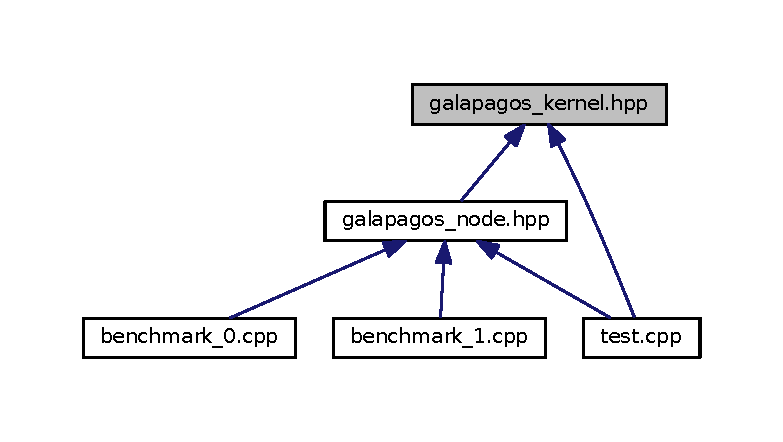
\includegraphics[width=350pt]{galapagos__kernel_8hpp__dep__incl}
\end{center}
\end{figure}
\subsection*{Classes}
\begin{DoxyCompactItemize}
\item 
class \hyperlink{classgalapagos_1_1kernel}{galapagos\+::kernel$<$ T $>$}
\begin{DoxyCompactList}\small\item\em Class for the Kernel wrapper. \end{DoxyCompactList}\end{DoxyCompactItemize}
\subsection*{Namespaces}
\begin{DoxyCompactItemize}
\item 
 \hyperlink{namespacegalapagos}{galapagos}
\end{DoxyCompactItemize}

\hypertarget{galapagos__local__router_8hpp}{}\section{galapagos\+\_\+local\+\_\+router.\+hpp File Reference}
\label{galapagos__local__router_8hpp}\index{galapagos\+\_\+local\+\_\+router.\+hpp@{galapagos\+\_\+local\+\_\+router.\+hpp}}
{\ttfamily \#include $<$map$>$}\\*
{\ttfamily \#include $<$assert.\+h$>$}\\*
{\ttfamily \#include \char`\"{}common.\+hpp\char`\"{}}\\*
{\ttfamily \#include $<$mutex$>$}\\*
{\ttfamily \#include $<$condition\+\_\+variable$>$}\\*
{\ttfamily \#include \char`\"{}galapagos\+\_\+interface.\+hpp\char`\"{}}\\*
Include dependency graph for galapagos\+\_\+local\+\_\+router.\+hpp\+:
\nopagebreak
\begin{figure}[H]
\begin{center}
\leavevmode
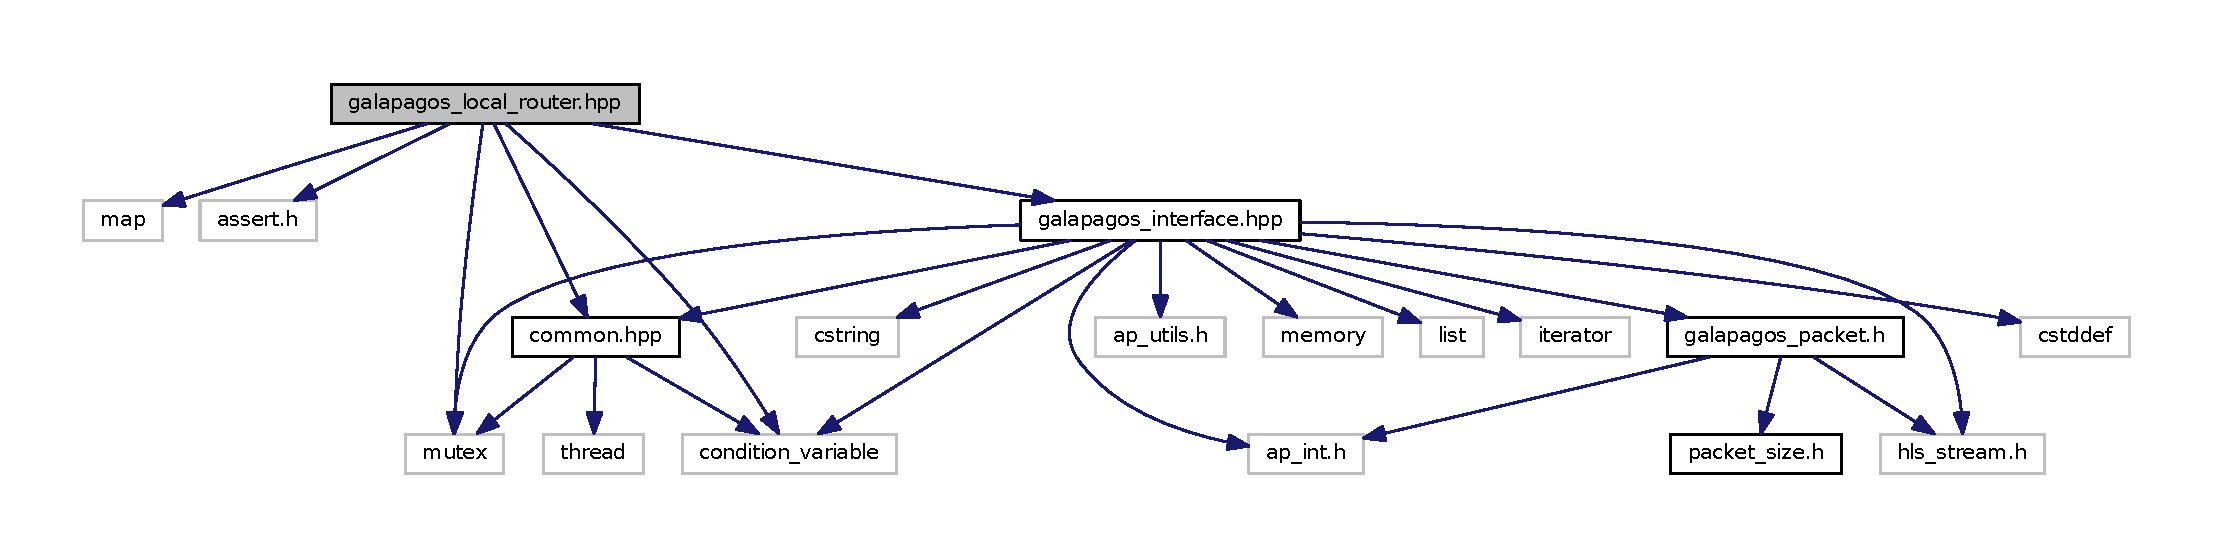
\includegraphics[width=350pt]{galapagos__local__router_8hpp__incl}
\end{center}
\end{figure}
This graph shows which files directly or indirectly include this file\+:
\nopagebreak
\begin{figure}[H]
\begin{center}
\leavevmode
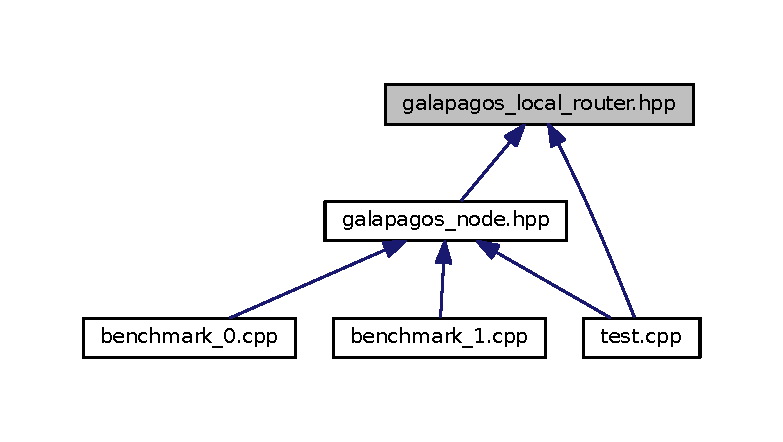
\includegraphics[width=350pt]{galapagos__local__router_8hpp__dep__incl}
\end{center}
\end{figure}
\subsection*{Classes}
\begin{DoxyCompactItemize}
\item 
class \hyperlink{classgalapagos_1_1local__router}{galapagos\+::local\+\_\+router$<$ T $>$}
\begin{DoxyCompactList}\small\item\em Class for the \hyperlink{classgalapagos_1_1local__router}{local\+\_\+router}. \end{DoxyCompactList}\end{DoxyCompactItemize}
\subsection*{Namespaces}
\begin{DoxyCompactItemize}
\item 
 \hyperlink{namespacegalapagos}{galapagos}
\end{DoxyCompactItemize}
\subsection*{Enumerations}
\begin{DoxyCompactItemize}
\item 
enum \hyperlink{galapagos__local__router_8hpp_af92acc2b81d20bf106a155c40d77aaee}{ext\+\_\+port} \{ \hyperlink{galapagos__local__router_8hpp_af92acc2b81d20bf106a155c40d77aaeeab6f81eb2559699fde2e883dec9bab5e7}{N\+E\+T\+W\+O\+R\+K\+\_\+\+E\+X\+T\+\_\+\+I\+N\+D\+EX}
 \}
\end{DoxyCompactItemize}


\subsection{Enumeration Type Documentation}
\index{galapagos\+\_\+local\+\_\+router.\+hpp@{galapagos\+\_\+local\+\_\+router.\+hpp}!ext\+\_\+port@{ext\+\_\+port}}
\index{ext\+\_\+port@{ext\+\_\+port}!galapagos\+\_\+local\+\_\+router.\+hpp@{galapagos\+\_\+local\+\_\+router.\+hpp}}
\subsubsection[{\texorpdfstring{ext\+\_\+port}{ext_port}}]{\setlength{\rightskip}{0pt plus 5cm}enum {\bf ext\+\_\+port}}\hypertarget{galapagos__local__router_8hpp_af92acc2b81d20bf106a155c40d77aaee}{}\label{galapagos__local__router_8hpp_af92acc2b81d20bf106a155c40d77aaee}
external port indices all external ports, , currently just have network but can be more (e.\+g P\+C\+Ie) \begin{Desc}
\item[Enumerator]\par
\begin{description}
\index{N\+E\+T\+W\+O\+R\+K\+\_\+\+E\+X\+T\+\_\+\+I\+N\+D\+EX@{N\+E\+T\+W\+O\+R\+K\+\_\+\+E\+X\+T\+\_\+\+I\+N\+D\+EX}!galapagos\+\_\+local\+\_\+router.\+hpp@{galapagos\+\_\+local\+\_\+router.\+hpp}}\index{galapagos\+\_\+local\+\_\+router.\+hpp@{galapagos\+\_\+local\+\_\+router.\+hpp}!N\+E\+T\+W\+O\+R\+K\+\_\+\+E\+X\+T\+\_\+\+I\+N\+D\+EX@{N\+E\+T\+W\+O\+R\+K\+\_\+\+E\+X\+T\+\_\+\+I\+N\+D\+EX}}\item[{\em 
N\+E\+T\+W\+O\+R\+K\+\_\+\+E\+X\+T\+\_\+\+I\+N\+D\+EX\hypertarget{galapagos__local__router_8hpp_af92acc2b81d20bf106a155c40d77aaeeab6f81eb2559699fde2e883dec9bab5e7}{}\label{galapagos__local__router_8hpp_af92acc2b81d20bf106a155c40d77aaeeab6f81eb2559699fde2e883dec9bab5e7}
}]\end{description}
\end{Desc}

\hypertarget{galapagos__n__to__one__router_8hpp}{}\section{galapagos\+\_\+n\+\_\+to\+\_\+one\+\_\+router.\+hpp File Reference}
\label{galapagos__n__to__one__router_8hpp}\index{galapagos\+\_\+n\+\_\+to\+\_\+one\+\_\+router.\+hpp@{galapagos\+\_\+n\+\_\+to\+\_\+one\+\_\+router.\+hpp}}
{\ttfamily \#include \char`\"{}common.\+hpp\char`\"{}}\\*
Include dependency graph for galapagos\+\_\+n\+\_\+to\+\_\+one\+\_\+router.\+hpp\+:
\nopagebreak
\begin{figure}[H]
\begin{center}
\leavevmode
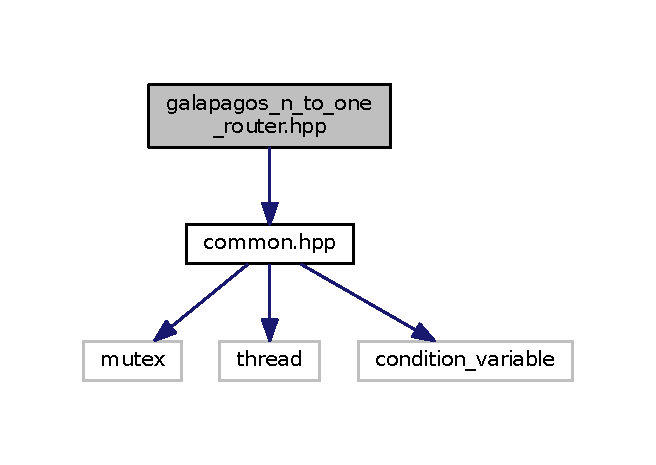
\includegraphics[width=315pt]{galapagos__n__to__one__router_8hpp__incl}
\end{center}
\end{figure}
This graph shows which files directly or indirectly include this file\+:
\nopagebreak
\begin{figure}[H]
\begin{center}
\leavevmode
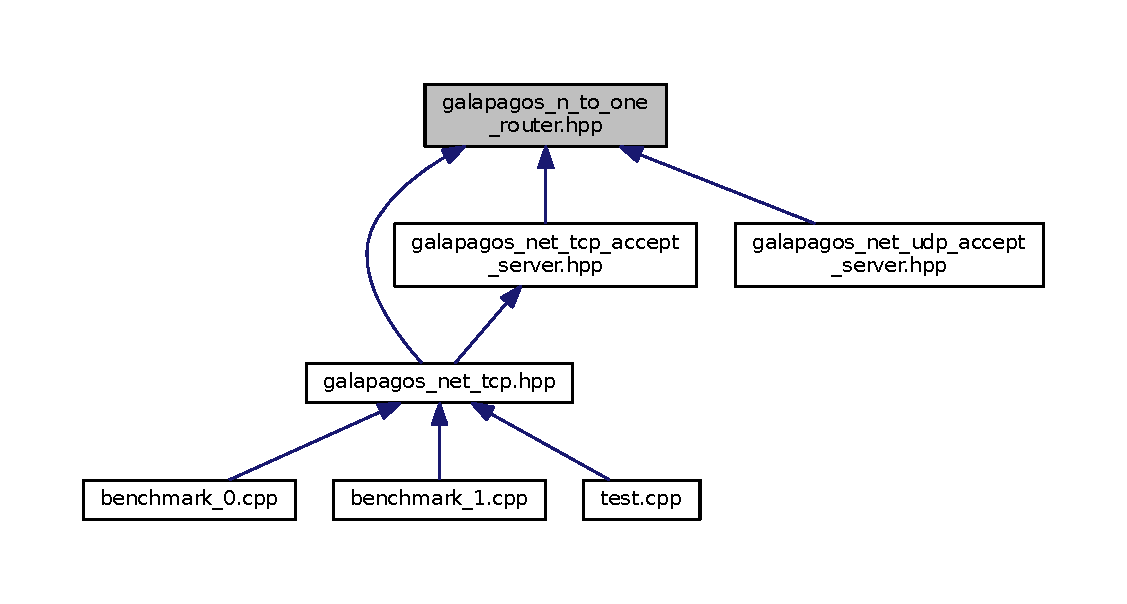
\includegraphics[width=350pt]{galapagos__n__to__one__router_8hpp__dep__incl}
\end{center}
\end{figure}
\subsection*{Classes}
\begin{DoxyCompactItemize}
\item 
class \hyperlink{classgalapagos_1_1n__to__one__router}{galapagos\+::n\+\_\+to\+\_\+one\+\_\+router$<$ T $>$}
\begin{DoxyCompactList}\small\item\em Class for the \hyperlink{classgalapagos_1_1n__to__one__router}{n\+\_\+to\+\_\+one\+\_\+router}. \end{DoxyCompactList}\end{DoxyCompactItemize}
\subsection*{Namespaces}
\begin{DoxyCompactItemize}
\item 
 \hyperlink{namespacegalapagos}{galapagos}
\end{DoxyCompactItemize}

\hypertarget{galapagos__net__tcp_8hpp}{}\section{galapagos\+\_\+net\+\_\+tcp.\+hpp File Reference}
\label{galapagos__net__tcp_8hpp}\index{galapagos\+\_\+net\+\_\+tcp.\+hpp@{galapagos\+\_\+net\+\_\+tcp.\+hpp}}
{\ttfamily \#include $<$boost/thread/locks.\+hpp$>$}\\*
{\ttfamily \#include $<$boost/thread/shared\+\_\+mutex.\+hpp$>$}\\*
{\ttfamily \#include $<$cstdlib$>$}\\*
{\ttfamily \#include $<$iostream$>$}\\*
{\ttfamily \#include $<$thread$>$}\\*
{\ttfamily \#include $<$memory$>$}\\*
{\ttfamily \#include $<$utility$>$}\\*
{\ttfamily \#include $<$boost/asio.\+hpp$>$}\\*
{\ttfamily \#include \char`\"{}common.\+hpp\char`\"{}}\\*
{\ttfamily \#include \char`\"{}galapagos\+\_\+interface.\+hpp\char`\"{}}\\*
{\ttfamily \#include \char`\"{}galapagos\+\_\+n\+\_\+to\+\_\+one\+\_\+router.\+hpp\char`\"{}}\\*
{\ttfamily \#include \char`\"{}galapagos\+\_\+net\+\_\+tcp\+\_\+session.\+hpp\char`\"{}}\\*
{\ttfamily \#include \char`\"{}galapagos\+\_\+net\+\_\+tcp\+\_\+accept\+\_\+server.\+hpp\char`\"{}}\\*
{\ttfamily \#include \char`\"{}galapagos\+\_\+net\+\_\+tcp\+\_\+server\+\_\+send.\+hpp\char`\"{}}\\*
{\ttfamily \#include \char`\"{}galapagos\+\_\+external\+\_\+driver.\+hpp\char`\"{}}\\*
Include dependency graph for galapagos\+\_\+net\+\_\+tcp.\+hpp\+:
\nopagebreak
\begin{figure}[H]
\begin{center}
\leavevmode
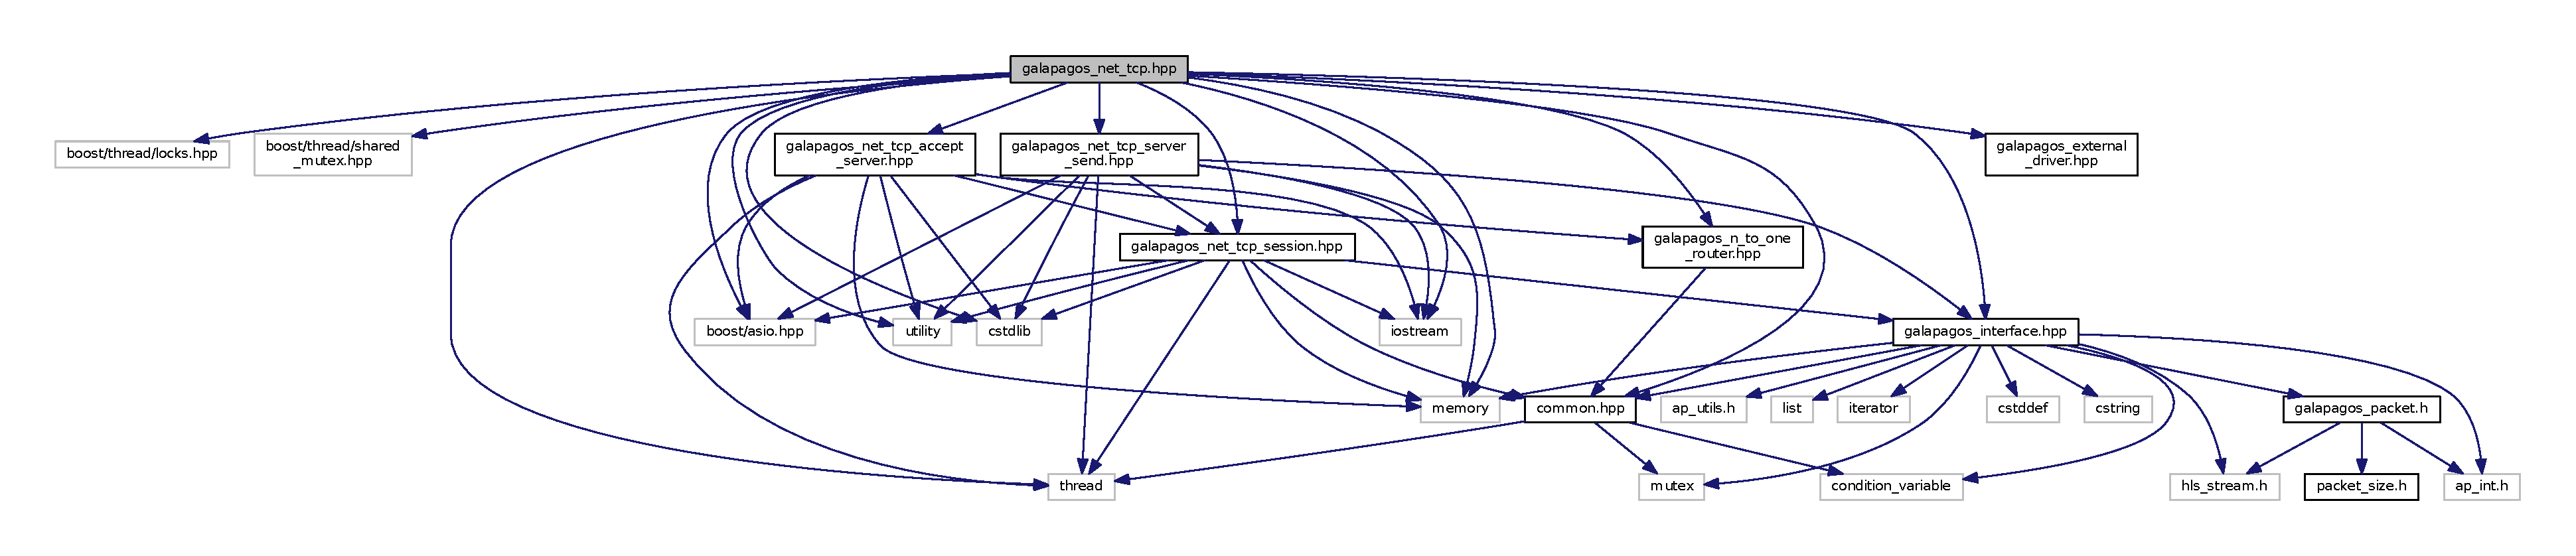
\includegraphics[width=350pt]{galapagos__net__tcp_8hpp__incl}
\end{center}
\end{figure}
This graph shows which files directly or indirectly include this file\+:
\nopagebreak
\begin{figure}[H]
\begin{center}
\leavevmode
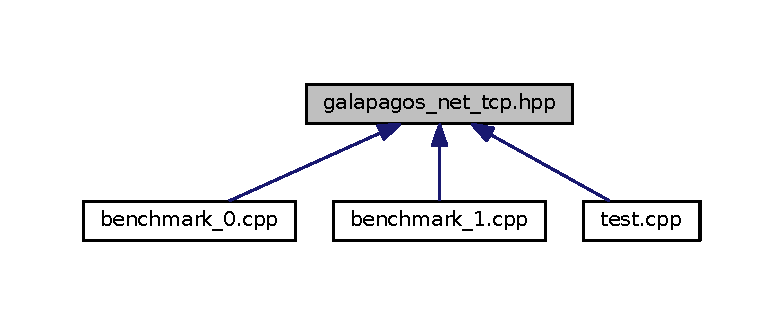
\includegraphics[width=350pt]{galapagos__net__tcp_8hpp__dep__incl}
\end{center}
\end{figure}
\subsection*{Classes}
\begin{DoxyCompactItemize}
\item 
class \hyperlink{classgalapagos_1_1net_1_1tcp}{galapagos\+::net\+::tcp$<$ T $>$}
\begin{DoxyCompactList}\small\item\em Class tcp driver. \end{DoxyCompactList}\end{DoxyCompactItemize}
\subsection*{Namespaces}
\begin{DoxyCompactItemize}
\item 
 \hyperlink{namespacegalapagos}{galapagos}
\item 
 \hyperlink{namespacegalapagos_1_1net}{galapagos\+::net}
\end{DoxyCompactItemize}

\hypertarget{galapagos__net__tcp__accept__server_8hpp}{}\section{galapagos\+\_\+net\+\_\+tcp\+\_\+accept\+\_\+server.\+hpp File Reference}
\label{galapagos__net__tcp__accept__server_8hpp}\index{galapagos\+\_\+net\+\_\+tcp\+\_\+accept\+\_\+server.\+hpp@{galapagos\+\_\+net\+\_\+tcp\+\_\+accept\+\_\+server.\+hpp}}
{\ttfamily \#include $<$cstdlib$>$}\\*
{\ttfamily \#include $<$iostream$>$}\\*
{\ttfamily \#include $<$thread$>$}\\*
{\ttfamily \#include $<$memory$>$}\\*
{\ttfamily \#include $<$utility$>$}\\*
{\ttfamily \#include $<$boost/asio.\+hpp$>$}\\*
{\ttfamily \#include \char`\"{}galapagos\+\_\+n\+\_\+to\+\_\+one\+\_\+router.\+hpp\char`\"{}}\\*
{\ttfamily \#include \char`\"{}galapagos\+\_\+net\+\_\+tcp\+\_\+session.\+hpp\char`\"{}}\\*
Include dependency graph for galapagos\+\_\+net\+\_\+tcp\+\_\+accept\+\_\+server.\+hpp\+:
\nopagebreak
\begin{figure}[H]
\begin{center}
\leavevmode
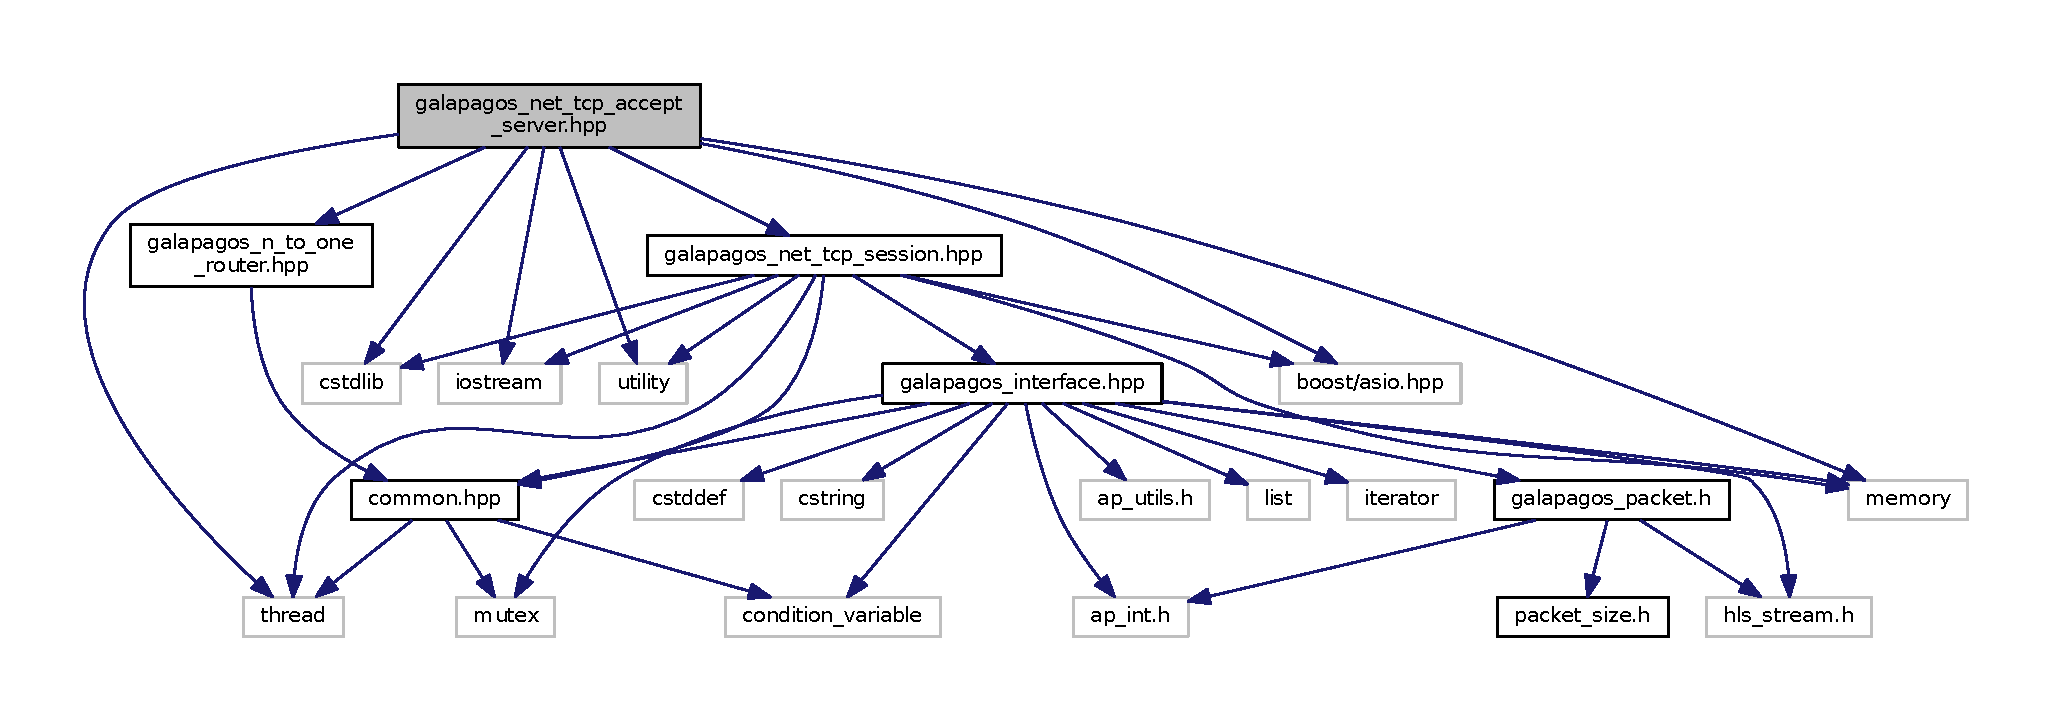
\includegraphics[width=350pt]{galapagos__net__tcp__accept__server_8hpp__incl}
\end{center}
\end{figure}
This graph shows which files directly or indirectly include this file\+:
\nopagebreak
\begin{figure}[H]
\begin{center}
\leavevmode
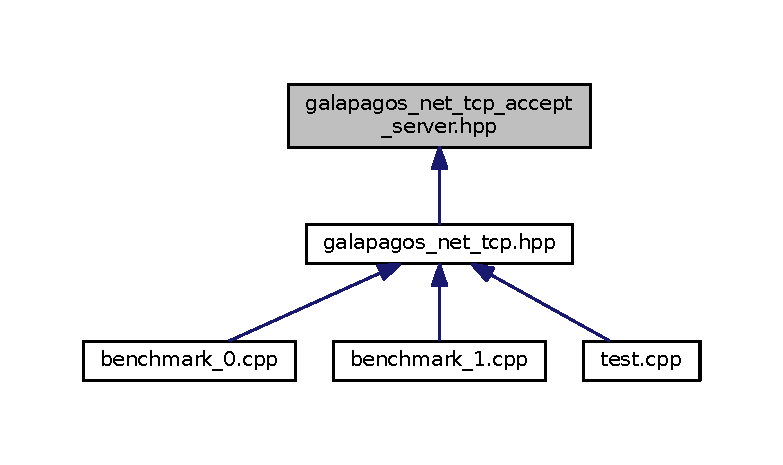
\includegraphics[width=350pt]{galapagos__net__tcp__accept__server_8hpp__dep__incl}
\end{center}
\end{figure}
\subsection*{Classes}
\begin{DoxyCompactItemize}
\item 
class \hyperlink{classgalapagos_1_1net_1_1tcp__accept__server}{galapagos\+::net\+::tcp\+\_\+accept\+\_\+server$<$ T $>$}
\end{DoxyCompactItemize}
\subsection*{Namespaces}
\begin{DoxyCompactItemize}
\item 
 \hyperlink{namespacegalapagos}{galapagos}
\item 
 \hyperlink{namespacegalapagos_1_1net}{galapagos\+::net}
\end{DoxyCompactItemize}
\subsection*{Macros}
\begin{DoxyCompactItemize}
\item 
\#define \hyperlink{galapagos__net__tcp__accept__server_8hpp_ac57497120dfa52f05f0e966cef63327a}{\+\_\+\+\_\+\+G\+A\+L\+A\+P\+A\+G\+O\+S\+\_\+\+N\+E\+T\+\_\+\+T\+C\+P\+\_\+\+A\+C\+C\+E\+P\+T\+\_\+\+S\+E\+R\+V\+E\+R\+\_\+\+H\+PP}
\end{DoxyCompactItemize}


\subsection{Macro Definition Documentation}
\index{galapagos\+\_\+net\+\_\+tcp\+\_\+accept\+\_\+server.\+hpp@{galapagos\+\_\+net\+\_\+tcp\+\_\+accept\+\_\+server.\+hpp}!\+\_\+\+\_\+\+G\+A\+L\+A\+P\+A\+G\+O\+S\+\_\+\+N\+E\+T\+\_\+\+T\+C\+P\+\_\+\+A\+C\+C\+E\+P\+T\+\_\+\+S\+E\+R\+V\+E\+R\+\_\+\+H\+PP@{\+\_\+\+\_\+\+G\+A\+L\+A\+P\+A\+G\+O\+S\+\_\+\+N\+E\+T\+\_\+\+T\+C\+P\+\_\+\+A\+C\+C\+E\+P\+T\+\_\+\+S\+E\+R\+V\+E\+R\+\_\+\+H\+PP}}
\index{\+\_\+\+\_\+\+G\+A\+L\+A\+P\+A\+G\+O\+S\+\_\+\+N\+E\+T\+\_\+\+T\+C\+P\+\_\+\+A\+C\+C\+E\+P\+T\+\_\+\+S\+E\+R\+V\+E\+R\+\_\+\+H\+PP@{\+\_\+\+\_\+\+G\+A\+L\+A\+P\+A\+G\+O\+S\+\_\+\+N\+E\+T\+\_\+\+T\+C\+P\+\_\+\+A\+C\+C\+E\+P\+T\+\_\+\+S\+E\+R\+V\+E\+R\+\_\+\+H\+PP}!galapagos\+\_\+net\+\_\+tcp\+\_\+accept\+\_\+server.\+hpp@{galapagos\+\_\+net\+\_\+tcp\+\_\+accept\+\_\+server.\+hpp}}
\subsubsection[{\texorpdfstring{\+\_\+\+\_\+\+G\+A\+L\+A\+P\+A\+G\+O\+S\+\_\+\+N\+E\+T\+\_\+\+T\+C\+P\+\_\+\+A\+C\+C\+E\+P\+T\+\_\+\+S\+E\+R\+V\+E\+R\+\_\+\+H\+PP}{__GALAPAGOS_NET_TCP_ACCEPT_SERVER_HPP}}]{\setlength{\rightskip}{0pt plus 5cm}\#define \+\_\+\+\_\+\+G\+A\+L\+A\+P\+A\+G\+O\+S\+\_\+\+N\+E\+T\+\_\+\+T\+C\+P\+\_\+\+A\+C\+C\+E\+P\+T\+\_\+\+S\+E\+R\+V\+E\+R\+\_\+\+H\+PP}\hypertarget{galapagos__net__tcp__accept__server_8hpp_ac57497120dfa52f05f0e966cef63327a}{}\label{galapagos__net__tcp__accept__server_8hpp_ac57497120dfa52f05f0e966cef63327a}

\hypertarget{galapagos__net__tcp__server__send_8hpp}{}\section{galapagos\+\_\+net\+\_\+tcp\+\_\+server\+\_\+send.\+hpp File Reference}
\label{galapagos__net__tcp__server__send_8hpp}\index{galapagos\+\_\+net\+\_\+tcp\+\_\+server\+\_\+send.\+hpp@{galapagos\+\_\+net\+\_\+tcp\+\_\+server\+\_\+send.\+hpp}}
{\ttfamily \#include $<$cstdlib$>$}\\*
{\ttfamily \#include $<$iostream$>$}\\*
{\ttfamily \#include $<$thread$>$}\\*
{\ttfamily \#include $<$memory$>$}\\*
{\ttfamily \#include $<$utility$>$}\\*
{\ttfamily \#include $<$boost/asio.\+hpp$>$}\\*
{\ttfamily \#include \char`\"{}galapagos\+\_\+interface.\+hpp\char`\"{}}\\*
{\ttfamily \#include \char`\"{}galapagos\+\_\+net\+\_\+tcp\+\_\+session.\+hpp\char`\"{}}\\*
Include dependency graph for galapagos\+\_\+net\+\_\+tcp\+\_\+server\+\_\+send.\+hpp\+:
\nopagebreak
\begin{figure}[H]
\begin{center}
\leavevmode
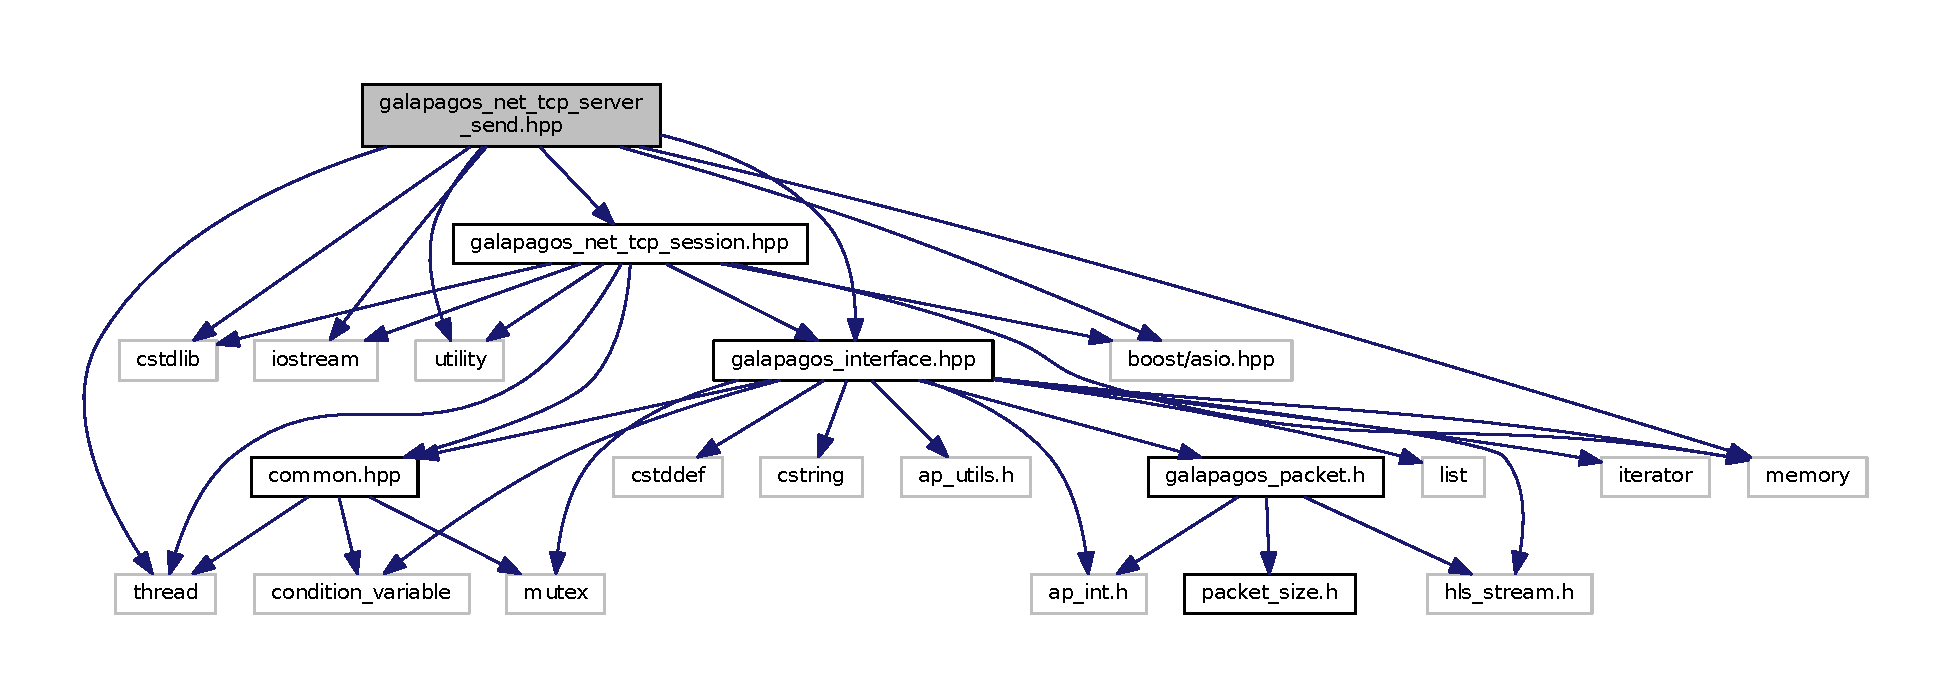
\includegraphics[width=350pt]{galapagos__net__tcp__server__send_8hpp__incl}
\end{center}
\end{figure}
This graph shows which files directly or indirectly include this file\+:
\nopagebreak
\begin{figure}[H]
\begin{center}
\leavevmode
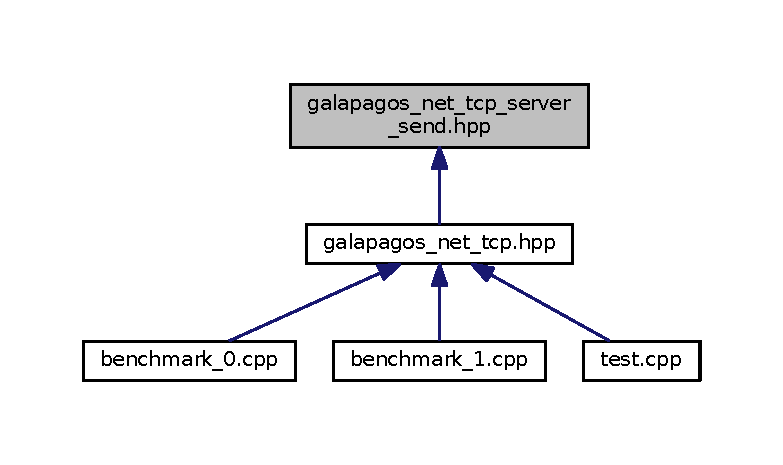
\includegraphics[width=350pt]{galapagos__net__tcp__server__send_8hpp__dep__incl}
\end{center}
\end{figure}
\subsection*{Classes}
\begin{DoxyCompactItemize}
\item 
class \hyperlink{classgalapagos_1_1net_1_1tcp__server__send}{galapagos\+::net\+::tcp\+\_\+server\+\_\+send$<$ T $>$}
\begin{DoxyCompactList}\small\item\em Class for the \hyperlink{classgalapagos_1_1net_1_1tcp__server__send}{tcp\+\_\+server\+\_\+send}, responsible for sending packets to sessions. \end{DoxyCompactList}\end{DoxyCompactItemize}
\subsection*{Namespaces}
\begin{DoxyCompactItemize}
\item 
 \hyperlink{namespacegalapagos}{galapagos}
\item 
 \hyperlink{namespacegalapagos_1_1net}{galapagos\+::net}
\end{DoxyCompactItemize}

\hypertarget{galapagos__net__tcp__session_8hpp}{}\section{galapagos\+\_\+net\+\_\+tcp\+\_\+session.\+hpp File Reference}
\label{galapagos__net__tcp__session_8hpp}\index{galapagos\+\_\+net\+\_\+tcp\+\_\+session.\+hpp@{galapagos\+\_\+net\+\_\+tcp\+\_\+session.\+hpp}}
{\ttfamily \#include $<$cstdlib$>$}\\*
{\ttfamily \#include $<$iostream$>$}\\*
{\ttfamily \#include $<$thread$>$}\\*
{\ttfamily \#include $<$memory$>$}\\*
{\ttfamily \#include $<$utility$>$}\\*
{\ttfamily \#include $<$boost/asio.\+hpp$>$}\\*
{\ttfamily \#include \char`\"{}galapagos\+\_\+interface.\+hpp\char`\"{}}\\*
{\ttfamily \#include \char`\"{}common.\+hpp\char`\"{}}\\*
Include dependency graph for galapagos\+\_\+net\+\_\+tcp\+\_\+session.\+hpp\+:
\nopagebreak
\begin{figure}[H]
\begin{center}
\leavevmode
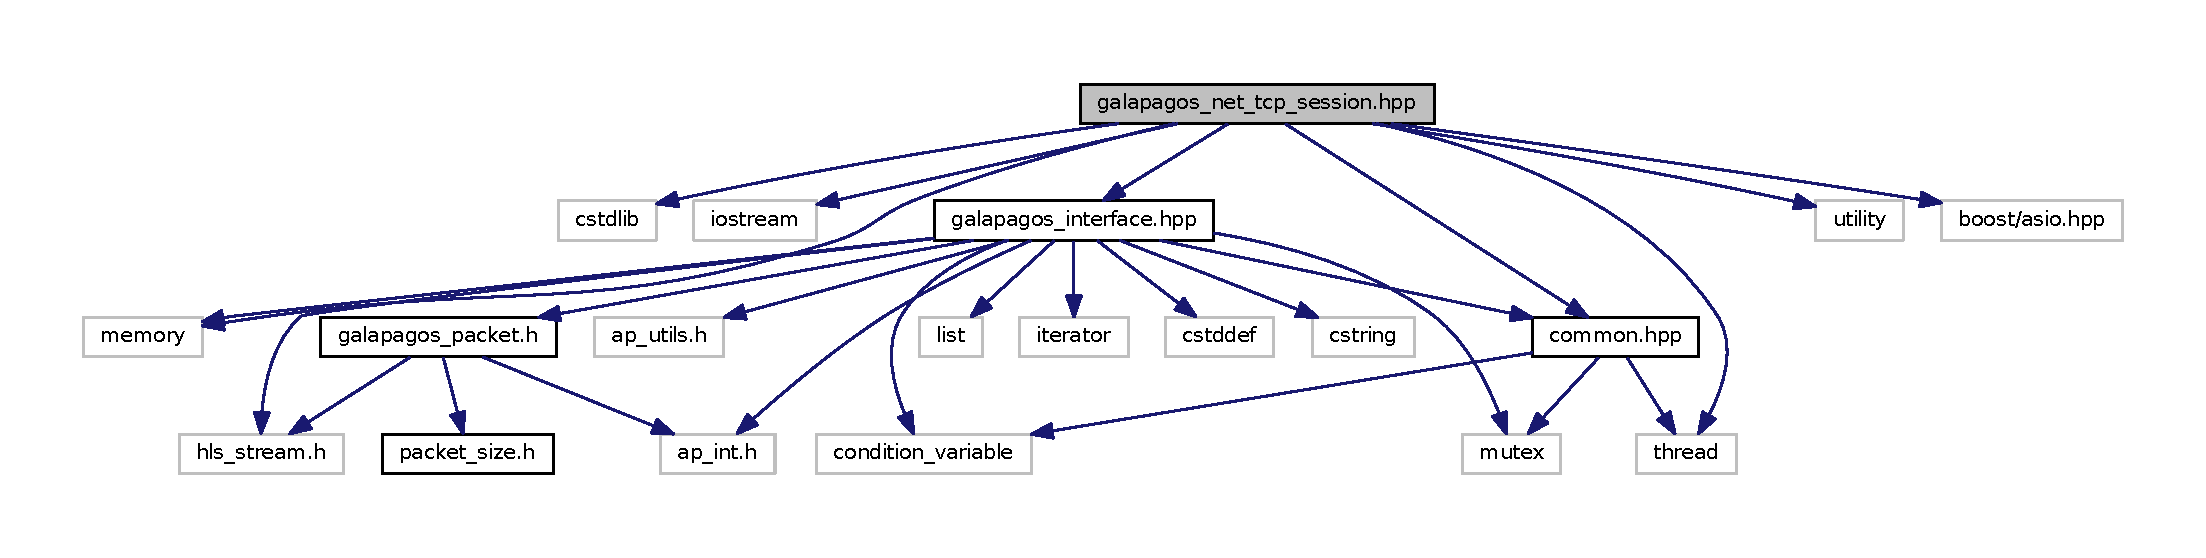
\includegraphics[width=350pt]{galapagos__net__tcp__session_8hpp__incl}
\end{center}
\end{figure}
This graph shows which files directly or indirectly include this file\+:
\nopagebreak
\begin{figure}[H]
\begin{center}
\leavevmode
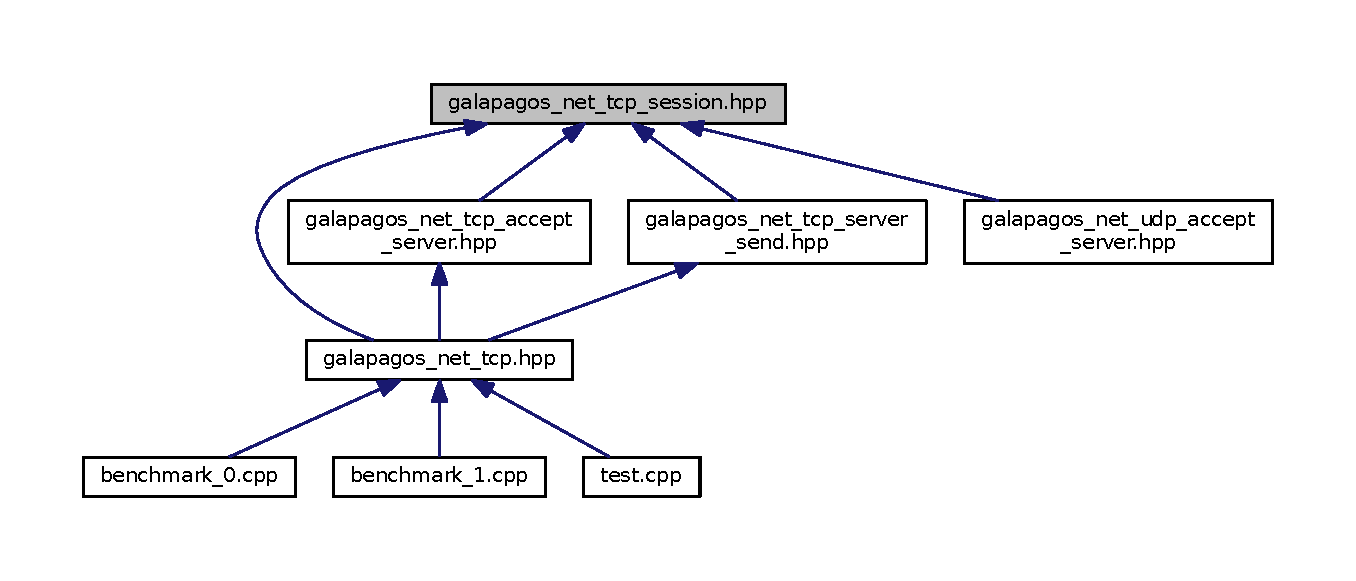
\includegraphics[width=350pt]{galapagos__net__tcp__session_8hpp__dep__incl}
\end{center}
\end{figure}
\subsection*{Classes}
\begin{DoxyCompactItemize}
\item 
class \hyperlink{classgalapagos_1_1net_1_1tcp__session}{galapagos\+::net\+::tcp\+\_\+session$<$ T $>$}
\begin{DoxyCompactList}\small\item\em Class for the \hyperlink{classgalapagos_1_1net_1_1tcp__session}{tcp\+\_\+session}. \end{DoxyCompactList}\item 
class \hyperlink{classgalapagos_1_1net_1_1tcp__session__container}{galapagos\+::net\+::tcp\+\_\+session\+\_\+container$<$ T $>$}
\begin{DoxyCompactList}\small\item\em Class for the session\+\_\+container. Addressable by dest. \end{DoxyCompactList}\end{DoxyCompactItemize}
\subsection*{Namespaces}
\begin{DoxyCompactItemize}
\item 
 \hyperlink{namespacegalapagos}{galapagos}
\item 
 \hyperlink{namespacegalapagos_1_1net}{galapagos\+::net}
\end{DoxyCompactItemize}

\hypertarget{galapagos__net__udp_8hpp}{}\section{galapagos\+\_\+net\+\_\+udp.\+hpp File Reference}
\label{galapagos__net__udp_8hpp}\index{galapagos\+\_\+net\+\_\+udp.\+hpp@{galapagos\+\_\+net\+\_\+udp.\+hpp}}
{\ttfamily \#include $<$boost/thread/locks.\+hpp$>$}\\*
{\ttfamily \#include $<$boost/thread/shared\+\_\+mutex.\+hpp$>$}\\*
{\ttfamily \#include $<$cstdlib$>$}\\*
{\ttfamily \#include $<$iostream$>$}\\*
{\ttfamily \#include $<$thread$>$}\\*
{\ttfamily \#include $<$memory$>$}\\*
{\ttfamily \#include $<$utility$>$}\\*
{\ttfamily \#include $<$boost/asio.\+hpp$>$}\\*
{\ttfamily \#include \char`\"{}common.\+hpp\char`\"{}}\\*
{\ttfamily \#include \char`\"{}galapagos\+\_\+interface.\+hpp\char`\"{}}\\*
{\ttfamily \#include \char`\"{}galapagos\+\_\+external\+\_\+driver.\+hpp\char`\"{}}\\*
Include dependency graph for galapagos\+\_\+net\+\_\+udp.\+hpp\+:
\nopagebreak
\begin{figure}[H]
\begin{center}
\leavevmode
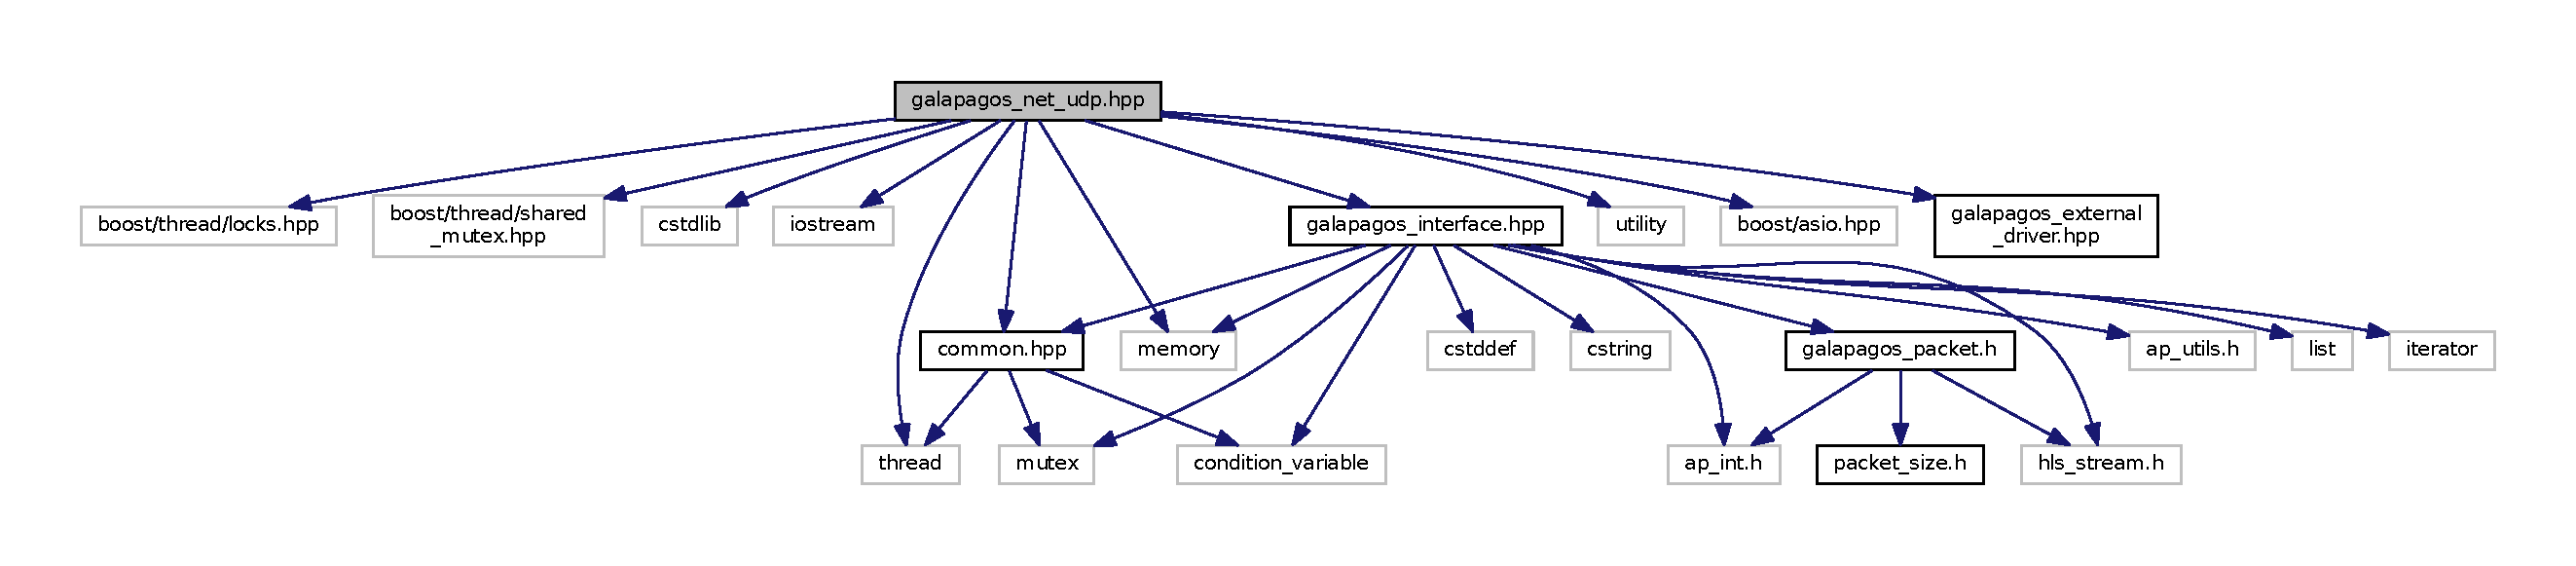
\includegraphics[width=350pt]{galapagos__net__udp_8hpp__incl}
\end{center}
\end{figure}
\subsection*{Classes}
\begin{DoxyCompactItemize}
\item 
class \hyperlink{classgalapagos_1_1net_1_1udp}{galapagos\+::net\+::udp$<$ T $>$}
\begin{DoxyCompactList}\small\item\em Class udp driver. \end{DoxyCompactList}\end{DoxyCompactItemize}
\subsection*{Namespaces}
\begin{DoxyCompactItemize}
\item 
 \hyperlink{namespacegalapagos}{galapagos}
\item 
 \hyperlink{namespacegalapagos_1_1net}{galapagos\+::net}
\end{DoxyCompactItemize}

\hypertarget{galapagos__net__udp__accept__server_8hpp}{}\section{galapagos\+\_\+net\+\_\+udp\+\_\+accept\+\_\+server.\+hpp File Reference}
\label{galapagos__net__udp__accept__server_8hpp}\index{galapagos\+\_\+net\+\_\+udp\+\_\+accept\+\_\+server.\+hpp@{galapagos\+\_\+net\+\_\+udp\+\_\+accept\+\_\+server.\+hpp}}
{\ttfamily \#include $<$cstdlib$>$}\\*
{\ttfamily \#include $<$iostream$>$}\\*
{\ttfamily \#include $<$thread$>$}\\*
{\ttfamily \#include $<$memory$>$}\\*
{\ttfamily \#include $<$utility$>$}\\*
{\ttfamily \#include $<$boost/asio.\+hpp$>$}\\*
{\ttfamily \#include \char`\"{}galapagos\+\_\+n\+\_\+to\+\_\+one\+\_\+router.\+hpp\char`\"{}}\\*
{\ttfamily \#include \char`\"{}galapagos\+\_\+net\+\_\+tcp\+\_\+session.\+hpp\char`\"{}}\\*
Include dependency graph for galapagos\+\_\+net\+\_\+udp\+\_\+accept\+\_\+server.\+hpp\+:
\nopagebreak
\begin{figure}[H]
\begin{center}
\leavevmode
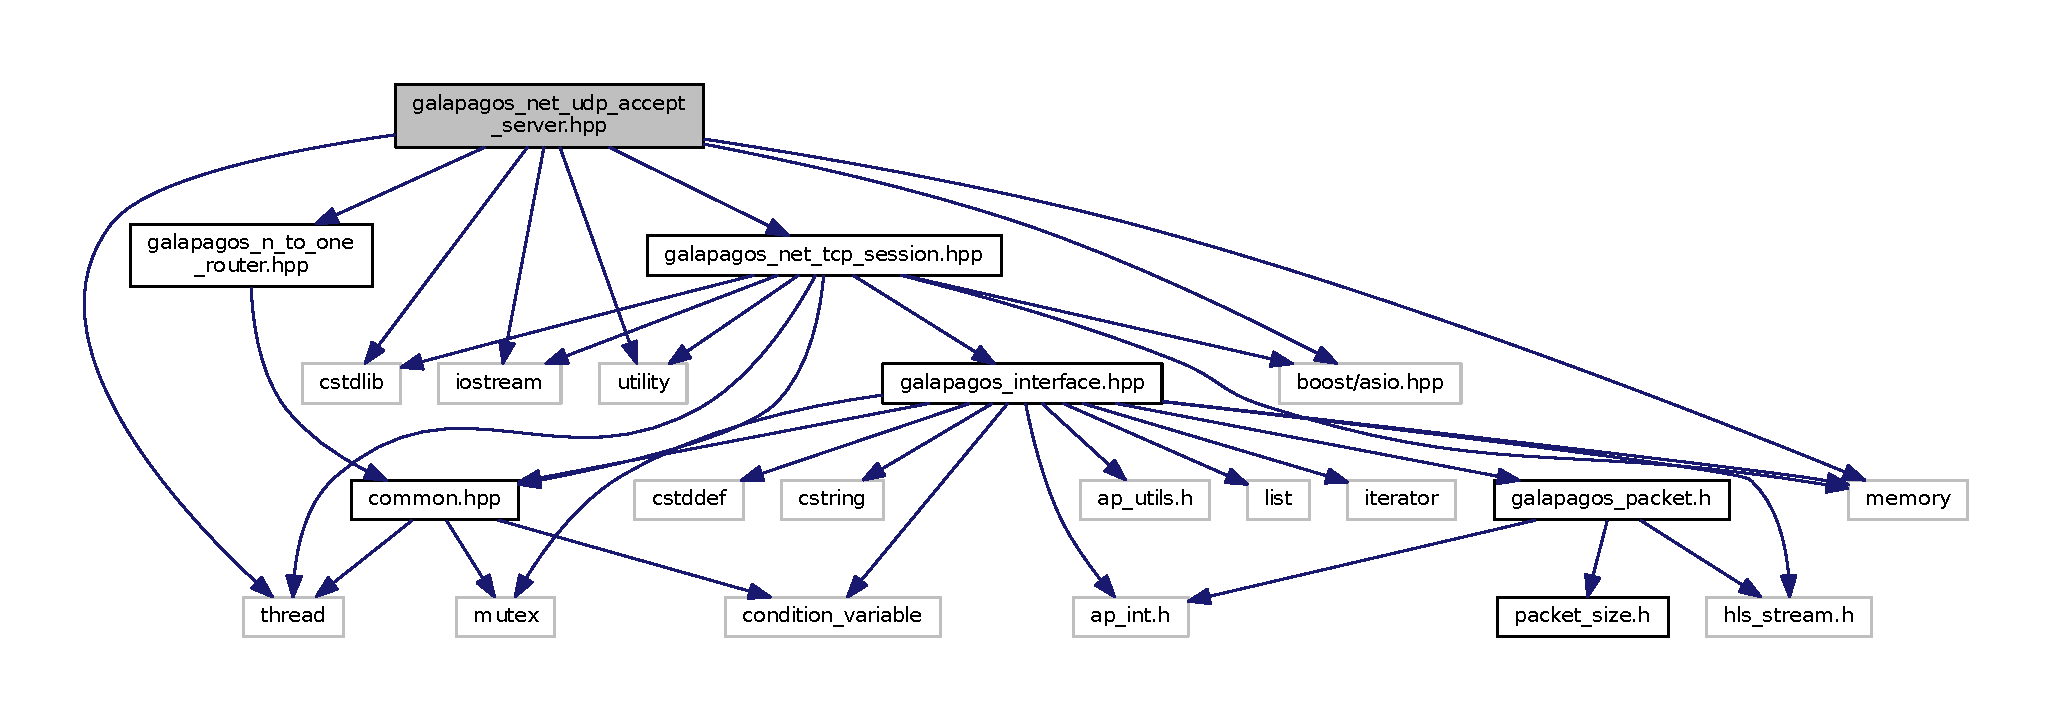
\includegraphics[width=350pt]{galapagos__net__udp__accept__server_8hpp__incl}
\end{center}
\end{figure}
\subsection*{Classes}
\begin{DoxyCompactItemize}
\item 
class \hyperlink{classgalapagos_1_1net_1_1tcp__accept__server}{galapagos\+::net\+::tcp\+\_\+accept\+\_\+server$<$ T $>$}
\end{DoxyCompactItemize}
\subsection*{Namespaces}
\begin{DoxyCompactItemize}
\item 
 \hyperlink{namespacegalapagos}{galapagos}
\item 
 \hyperlink{namespacegalapagos_1_1net}{galapagos\+::net}
\end{DoxyCompactItemize}
\subsection*{Macros}
\begin{DoxyCompactItemize}
\item 
\#define \hyperlink{galapagos__net__udp__accept__server_8hpp_ac57497120dfa52f05f0e966cef63327a}{\+\_\+\+\_\+\+G\+A\+L\+A\+P\+A\+G\+O\+S\+\_\+\+N\+E\+T\+\_\+\+T\+C\+P\+\_\+\+A\+C\+C\+E\+P\+T\+\_\+\+S\+E\+R\+V\+E\+R\+\_\+\+H\+PP}
\end{DoxyCompactItemize}


\subsection{Macro Definition Documentation}
\index{galapagos\+\_\+net\+\_\+udp\+\_\+accept\+\_\+server.\+hpp@{galapagos\+\_\+net\+\_\+udp\+\_\+accept\+\_\+server.\+hpp}!\+\_\+\+\_\+\+G\+A\+L\+A\+P\+A\+G\+O\+S\+\_\+\+N\+E\+T\+\_\+\+T\+C\+P\+\_\+\+A\+C\+C\+E\+P\+T\+\_\+\+S\+E\+R\+V\+E\+R\+\_\+\+H\+PP@{\+\_\+\+\_\+\+G\+A\+L\+A\+P\+A\+G\+O\+S\+\_\+\+N\+E\+T\+\_\+\+T\+C\+P\+\_\+\+A\+C\+C\+E\+P\+T\+\_\+\+S\+E\+R\+V\+E\+R\+\_\+\+H\+PP}}
\index{\+\_\+\+\_\+\+G\+A\+L\+A\+P\+A\+G\+O\+S\+\_\+\+N\+E\+T\+\_\+\+T\+C\+P\+\_\+\+A\+C\+C\+E\+P\+T\+\_\+\+S\+E\+R\+V\+E\+R\+\_\+\+H\+PP@{\+\_\+\+\_\+\+G\+A\+L\+A\+P\+A\+G\+O\+S\+\_\+\+N\+E\+T\+\_\+\+T\+C\+P\+\_\+\+A\+C\+C\+E\+P\+T\+\_\+\+S\+E\+R\+V\+E\+R\+\_\+\+H\+PP}!galapagos\+\_\+net\+\_\+udp\+\_\+accept\+\_\+server.\+hpp@{galapagos\+\_\+net\+\_\+udp\+\_\+accept\+\_\+server.\+hpp}}
\subsubsection[{\texorpdfstring{\+\_\+\+\_\+\+G\+A\+L\+A\+P\+A\+G\+O\+S\+\_\+\+N\+E\+T\+\_\+\+T\+C\+P\+\_\+\+A\+C\+C\+E\+P\+T\+\_\+\+S\+E\+R\+V\+E\+R\+\_\+\+H\+PP}{__GALAPAGOS_NET_TCP_ACCEPT_SERVER_HPP}}]{\setlength{\rightskip}{0pt plus 5cm}\#define \+\_\+\+\_\+\+G\+A\+L\+A\+P\+A\+G\+O\+S\+\_\+\+N\+E\+T\+\_\+\+T\+C\+P\+\_\+\+A\+C\+C\+E\+P\+T\+\_\+\+S\+E\+R\+V\+E\+R\+\_\+\+H\+PP}\hypertarget{galapagos__net__udp__accept__server_8hpp_ac57497120dfa52f05f0e966cef63327a}{}\label{galapagos__net__udp__accept__server_8hpp_ac57497120dfa52f05f0e966cef63327a}

\hypertarget{galapagos__node_8hpp}{}\section{galapagos\+\_\+node.\+hpp File Reference}
\label{galapagos__node_8hpp}\index{galapagos\+\_\+node.\+hpp@{galapagos\+\_\+node.\+hpp}}
{\ttfamily \#include $<$map$>$}\\*
{\ttfamily \#include $<$assert.\+h$>$}\\*
{\ttfamily \#include $<$boost/thread/locks.\+hpp$>$}\\*
{\ttfamily \#include $<$boost/thread/shared\+\_\+mutex.\+hpp$>$}\\*
{\ttfamily \#include \char`\"{}galapagos\+\_\+packet.\+h\char`\"{}}\\*
{\ttfamily \#include \char`\"{}galapagos\+\_\+interface.\+hpp\char`\"{}}\\*
{\ttfamily \#include \char`\"{}galapagos\+\_\+kernel.\+hpp\char`\"{}}\\*
{\ttfamily \#include \char`\"{}galapagos\+\_\+local\+\_\+router.\+hpp\char`\"{}}\\*
{\ttfamily \#include \char`\"{}galapagos\+\_\+external\+\_\+driver.\+hpp\char`\"{}}\\*
Include dependency graph for galapagos\+\_\+node.\+hpp\+:
\nopagebreak
\begin{figure}[H]
\begin{center}
\leavevmode
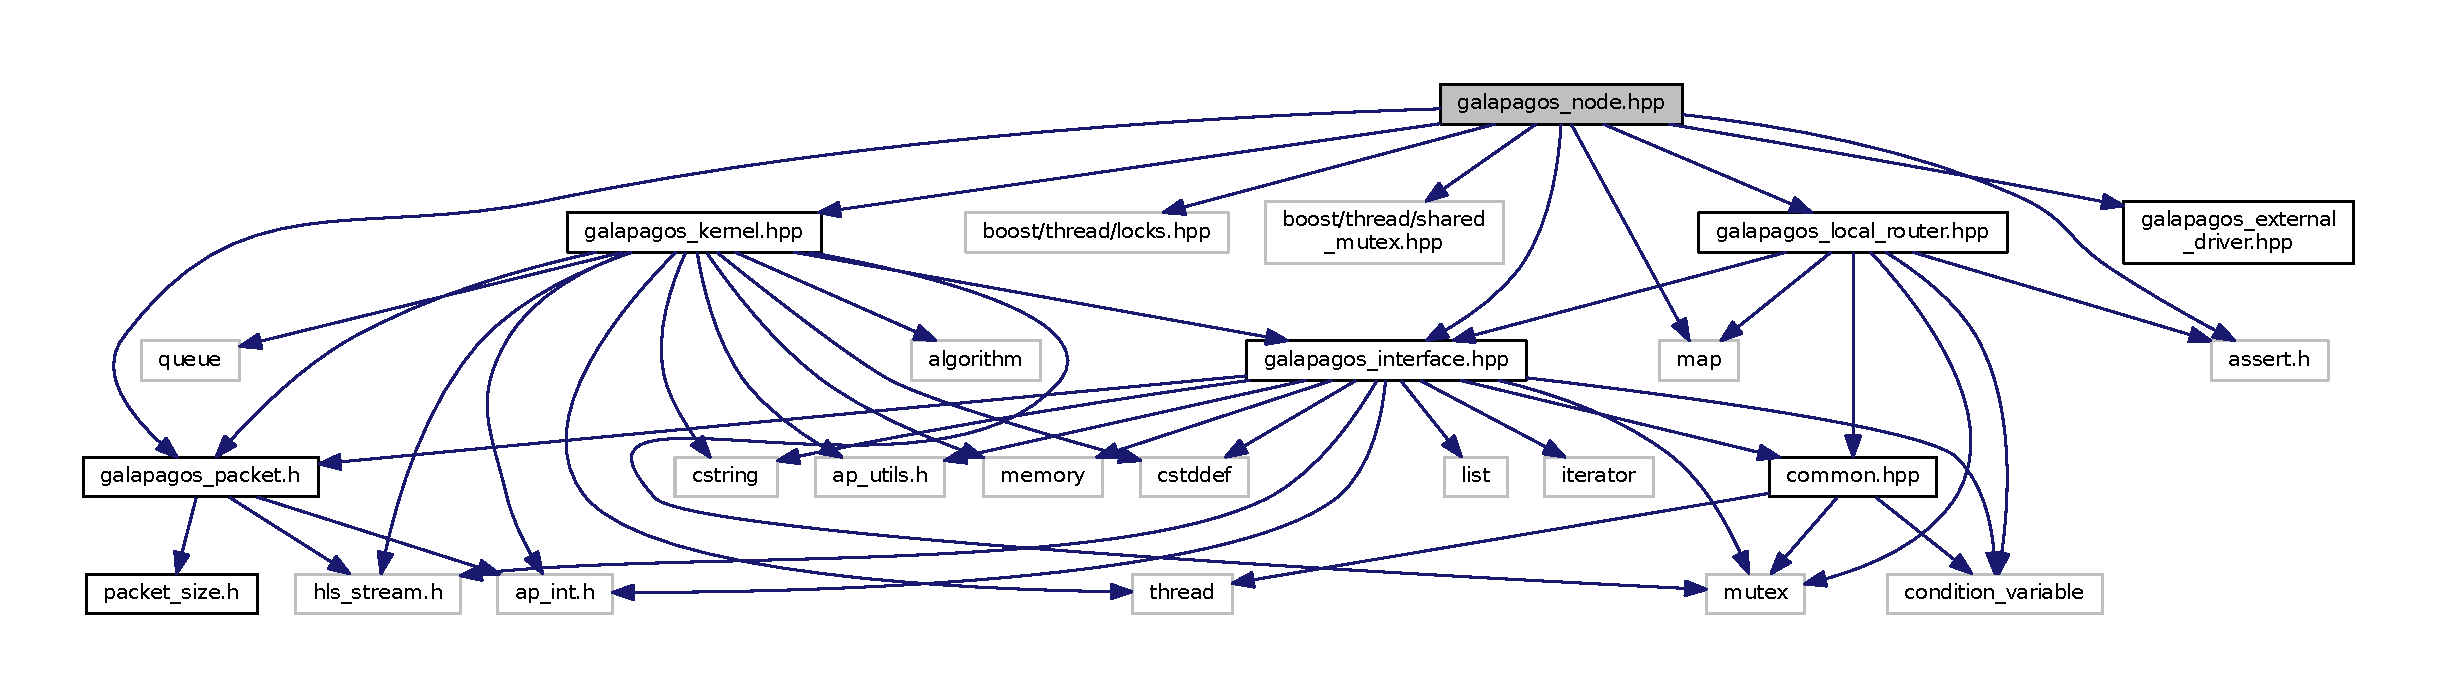
\includegraphics[width=350pt]{galapagos__node_8hpp__incl}
\end{center}
\end{figure}
This graph shows which files directly or indirectly include this file\+:
\nopagebreak
\begin{figure}[H]
\begin{center}
\leavevmode
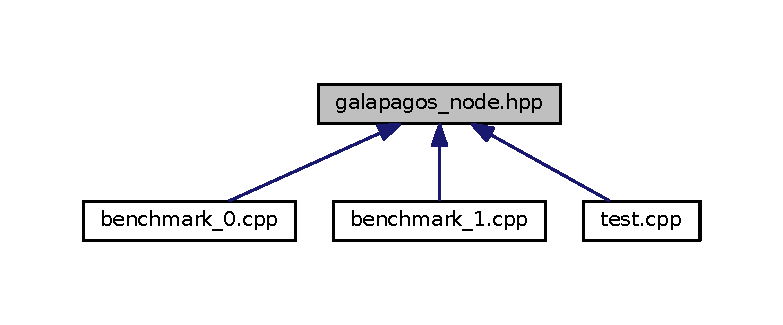
\includegraphics[width=350pt]{galapagos__node_8hpp__dep__incl}
\end{center}
\end{figure}
\subsection*{Classes}
\begin{DoxyCompactItemize}
\item 
class \hyperlink{classgalapagos_1_1node}{galapagos\+::node$<$ T $>$}
\end{DoxyCompactItemize}
\subsection*{Namespaces}
\begin{DoxyCompactItemize}
\item 
 \hyperlink{namespacegalapagos}{galapagos}
\end{DoxyCompactItemize}

\hypertarget{galapagos__packet_8h}{}\section{galapagos\+\_\+packet.\+h File Reference}
\label{galapagos__packet_8h}\index{galapagos\+\_\+packet.\+h@{galapagos\+\_\+packet.\+h}}
{\ttfamily \#include \char`\"{}hls\+\_\+stream.\+h\char`\"{}}\\*
{\ttfamily \#include \char`\"{}ap\+\_\+int.\+h\char`\"{}}\\*
{\ttfamily \#include \char`\"{}packet\+\_\+size.\+h\char`\"{}}\\*
Include dependency graph for galapagos\+\_\+packet.\+h\+:
\nopagebreak
\begin{figure}[H]
\begin{center}
\leavevmode
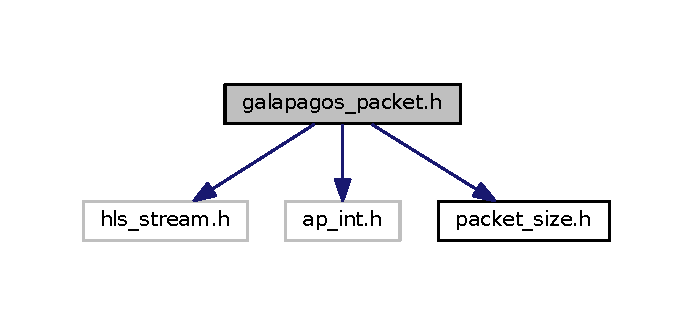
\includegraphics[width=333pt]{galapagos__packet_8h__incl}
\end{center}
\end{figure}
This graph shows which files directly or indirectly include this file\+:
\nopagebreak
\begin{figure}[H]
\begin{center}
\leavevmode
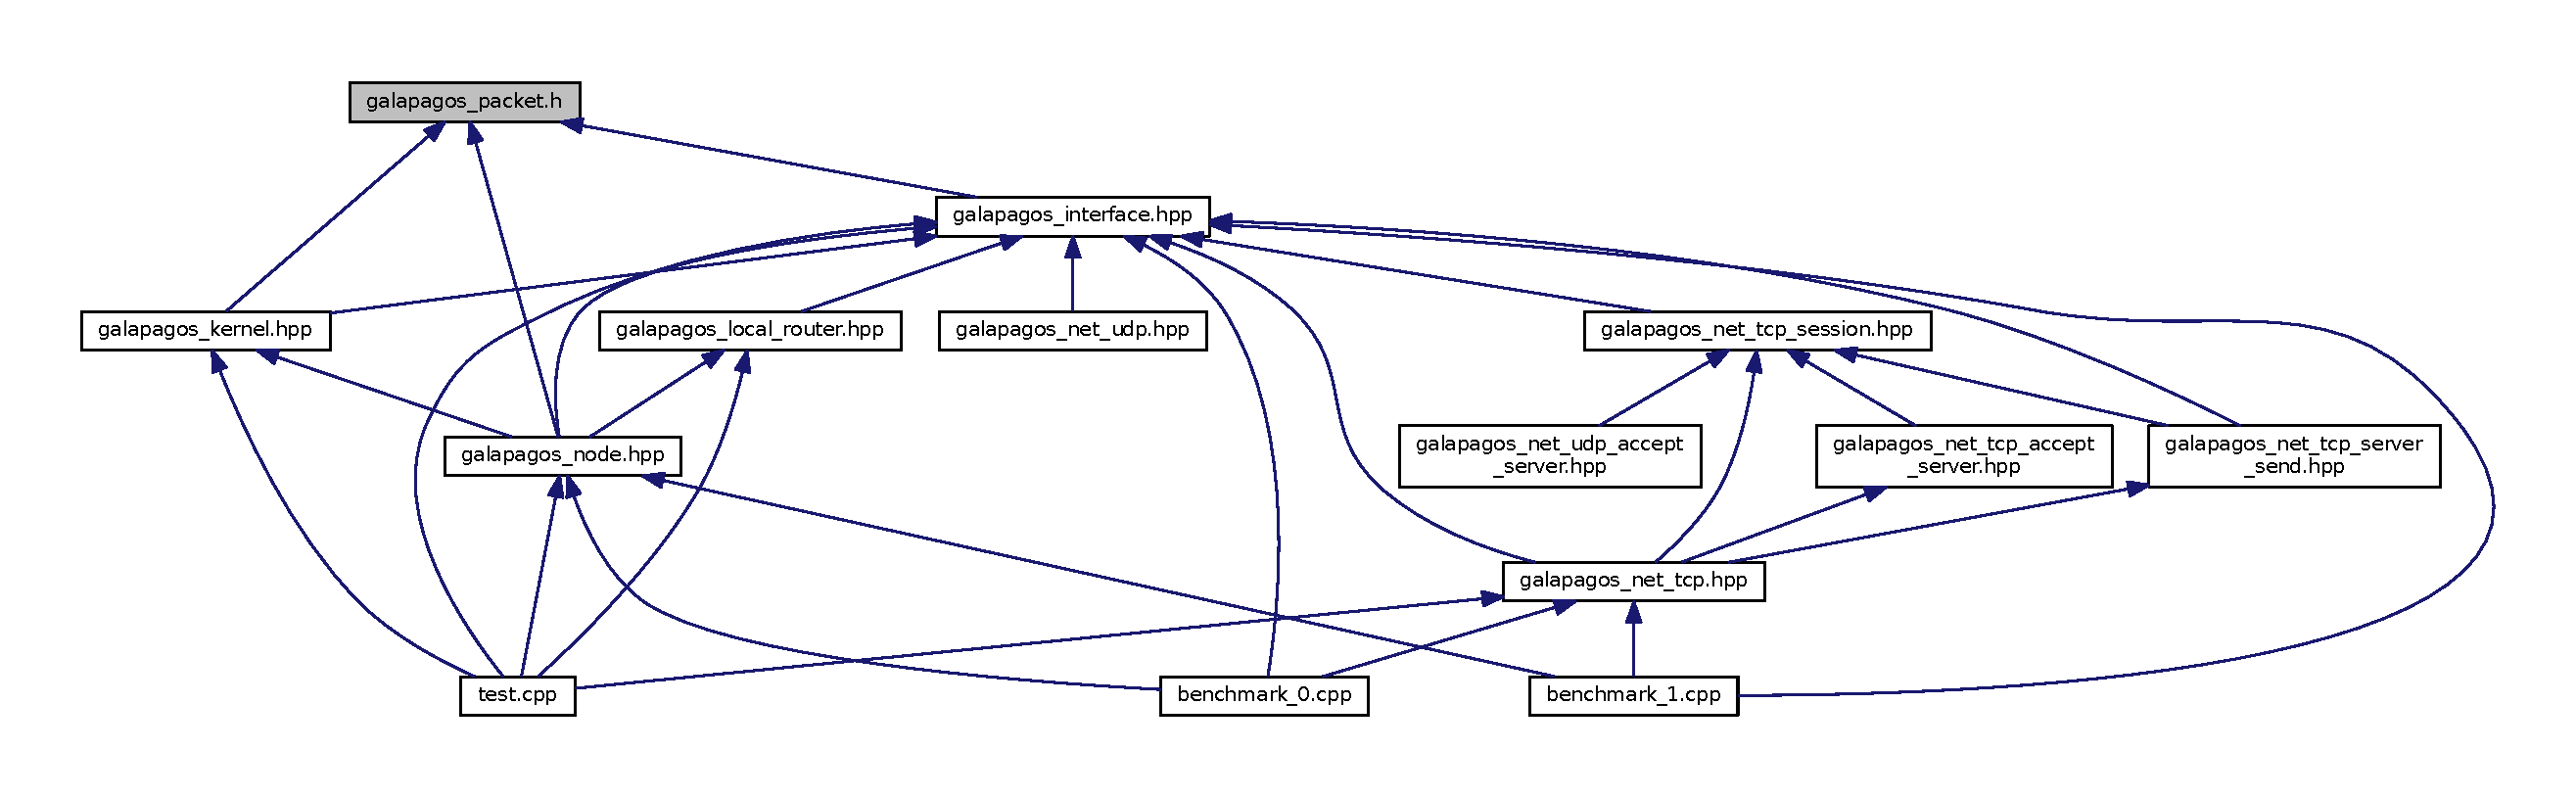
\includegraphics[width=350pt]{galapagos__packet_8h__dep__incl}
\end{center}
\end{figure}
\subsection*{Classes}
\begin{DoxyCompactItemize}
\item 
struct \hyperlink{structgalapagos_1_1stream__packet}{galapagos\+::stream\+\_\+packet$<$ T $>$}
\end{DoxyCompactItemize}
\subsection*{Namespaces}
\begin{DoxyCompactItemize}
\item 
 \hyperlink{namespacegalapagos}{galapagos}
\end{DoxyCompactItemize}
\subsection*{Macros}
\begin{DoxyCompactItemize}
\item 
\#define \hyperlink{galapagos__packet_8h_a225a4d42aa14ee4af829148d6fecee85}{K\+E\+E\+P\+\_\+\+A\+LL}~0xff
\end{DoxyCompactItemize}
\subsection*{Typedefs}
\begin{DoxyCompactItemize}
\item 
{\footnotesize template$<$typename T $>$ }\\using \hyperlink{namespacegalapagos_a151d65e2506da0745201fb1dae77b740}{galapagos\+::interface} = hls\+::stream$<$ \hyperlink{structgalapagos_1_1stream__packet}{galapagos\+::stream\+\_\+packet}$<$ \hyperlink{test_8cpp_a0658ceffa730c765d449bb3d21871b5f}{T} $>$ $>$
\item 
typedef \hyperlink{structgalapagos_1_1stream__packet}{galapagos\+::stream\+\_\+packet}$<$ ap\+\_\+uint$<$ \hyperlink{packet__size_8h_aaf115bf32d6740657027593bc293743c}{P\+A\+C\+K\+E\+T\+\_\+\+D\+A\+T\+A\+\_\+\+L\+E\+N\+G\+TH} $>$ $>$ \hyperlink{galapagos__packet_8h_a820cd44cf3f689bbf53bd38dfb5c91ca}{galapagos\+\_\+packet}
\item 
typedef hls\+::stream$<$ \hyperlink{galapagos__packet_8h_a820cd44cf3f689bbf53bd38dfb5c91ca}{galapagos\+\_\+packet} $>$ \hyperlink{galapagos__packet_8h_aeee9262148d04aca4deb758e2f40e51d}{galapagos\+\_\+interface}
\end{DoxyCompactItemize}
\subsection*{Functions}
\begin{DoxyCompactItemize}
\item 
ap\+\_\+uint$<$ \hyperlink{packet__size_8h_aaf115bf32d6740657027593bc293743c}{P\+A\+C\+K\+E\+T\+\_\+\+D\+A\+T\+A\+\_\+\+L\+E\+N\+G\+TH} $>$ \hyperlink{galapagos__packet_8h_abd8908a42ff059eaefe83cff21f932c4}{get\+\_\+header} (ap\+\_\+uint$<$ \hyperlink{packet__size_8h_a5e007ff81bb2779243ac4d9984a00dff}{P\+A\+C\+K\+E\+T\+\_\+\+D\+E\+S\+T\+\_\+\+L\+E\+N\+G\+TH} $>$ \+\_\+id, ap\+\_\+uint$<$ \hyperlink{packet__size_8h_a5e007ff81bb2779243ac4d9984a00dff}{P\+A\+C\+K\+E\+T\+\_\+\+D\+E\+S\+T\+\_\+\+L\+E\+N\+G\+TH} $>$ \+\_\+dest, ap\+\_\+uint$<$ \hyperlink{packet__size_8h_af5db3d603be0d574545c417ad0e0520d}{P\+A\+C\+K\+E\+T\+\_\+\+U\+S\+E\+R\+\_\+\+L\+E\+N\+G\+TH} $>$ \+\_\+size)
\end{DoxyCompactItemize}


\subsection{Macro Definition Documentation}
\index{galapagos\+\_\+packet.\+h@{galapagos\+\_\+packet.\+h}!K\+E\+E\+P\+\_\+\+A\+LL@{K\+E\+E\+P\+\_\+\+A\+LL}}
\index{K\+E\+E\+P\+\_\+\+A\+LL@{K\+E\+E\+P\+\_\+\+A\+LL}!galapagos\+\_\+packet.\+h@{galapagos\+\_\+packet.\+h}}
\subsubsection[{\texorpdfstring{K\+E\+E\+P\+\_\+\+A\+LL}{KEEP_ALL}}]{\setlength{\rightskip}{0pt plus 5cm}\#define K\+E\+E\+P\+\_\+\+A\+LL~0xff}\hypertarget{galapagos__packet_8h_a225a4d42aa14ee4af829148d6fecee85}{}\label{galapagos__packet_8h_a225a4d42aa14ee4af829148d6fecee85}


\subsection{Typedef Documentation}
\index{galapagos\+\_\+packet.\+h@{galapagos\+\_\+packet.\+h}!galapagos\+\_\+interface@{galapagos\+\_\+interface}}
\index{galapagos\+\_\+interface@{galapagos\+\_\+interface}!galapagos\+\_\+packet.\+h@{galapagos\+\_\+packet.\+h}}
\subsubsection[{\texorpdfstring{galapagos\+\_\+interface}{galapagos_interface}}]{\setlength{\rightskip}{0pt plus 5cm}typedef hls\+::stream$<${\bf galapagos\+\_\+packet}$>$ {\bf galapagos\+\_\+interface}}\hypertarget{galapagos__packet_8h_aeee9262148d04aca4deb758e2f40e51d}{}\label{galapagos__packet_8h_aeee9262148d04aca4deb758e2f40e51d}
\index{galapagos\+\_\+packet.\+h@{galapagos\+\_\+packet.\+h}!galapagos\+\_\+packet@{galapagos\+\_\+packet}}
\index{galapagos\+\_\+packet@{galapagos\+\_\+packet}!galapagos\+\_\+packet.\+h@{galapagos\+\_\+packet.\+h}}
\subsubsection[{\texorpdfstring{galapagos\+\_\+packet}{galapagos_packet}}]{\setlength{\rightskip}{0pt plus 5cm}typedef {\bf galapagos\+::stream\+\_\+packet}$<$ap\+\_\+uint$<${\bf P\+A\+C\+K\+E\+T\+\_\+\+D\+A\+T\+A\+\_\+\+L\+E\+N\+G\+TH}$>$ $>$ {\bf galapagos\+\_\+packet}}\hypertarget{galapagos__packet_8h_a820cd44cf3f689bbf53bd38dfb5c91ca}{}\label{galapagos__packet_8h_a820cd44cf3f689bbf53bd38dfb5c91ca}


\subsection{Function Documentation}
\index{galapagos\+\_\+packet.\+h@{galapagos\+\_\+packet.\+h}!get\+\_\+header@{get\+\_\+header}}
\index{get\+\_\+header@{get\+\_\+header}!galapagos\+\_\+packet.\+h@{galapagos\+\_\+packet.\+h}}
\subsubsection[{\texorpdfstring{get\+\_\+header(ap\+\_\+uint$<$ P\+A\+C\+K\+E\+T\+\_\+\+D\+E\+S\+T\+\_\+\+L\+E\+N\+G\+T\+H $>$ \+\_\+id, ap\+\_\+uint$<$ P\+A\+C\+K\+E\+T\+\_\+\+D\+E\+S\+T\+\_\+\+L\+E\+N\+G\+T\+H $>$ \+\_\+dest, ap\+\_\+uint$<$ P\+A\+C\+K\+E\+T\+\_\+\+U\+S\+E\+R\+\_\+\+L\+E\+N\+G\+T\+H $>$ \+\_\+size)}{get_header(ap_uint< PACKET_DEST_LENGTH > _id, ap_uint< PACKET_DEST_LENGTH > _dest, ap_uint< PACKET_USER_LENGTH > _size)}}]{\setlength{\rightskip}{0pt plus 5cm}ap\+\_\+uint$<${\bf P\+A\+C\+K\+E\+T\+\_\+\+D\+A\+T\+A\+\_\+\+L\+E\+N\+G\+TH}$>$ get\+\_\+header (
\begin{DoxyParamCaption}
\item[{ap\+\_\+uint$<$ {\bf P\+A\+C\+K\+E\+T\+\_\+\+D\+E\+S\+T\+\_\+\+L\+E\+N\+G\+TH} $>$}]{\+\_\+id, }
\item[{ap\+\_\+uint$<$ {\bf P\+A\+C\+K\+E\+T\+\_\+\+D\+E\+S\+T\+\_\+\+L\+E\+N\+G\+TH} $>$}]{\+\_\+dest, }
\item[{ap\+\_\+uint$<$ {\bf P\+A\+C\+K\+E\+T\+\_\+\+U\+S\+E\+R\+\_\+\+L\+E\+N\+G\+TH} $>$}]{\+\_\+size}
\end{DoxyParamCaption}
)\hspace{0.3cm}{\ttfamily [inline]}}\hypertarget{galapagos__packet_8h_abd8908a42ff059eaefe83cff21f932c4}{}\label{galapagos__packet_8h_abd8908a42ff059eaefe83cff21f932c4}

\hypertarget{packet__size_8h}{}\section{packet\+\_\+size.\+h File Reference}
\label{packet__size_8h}\index{packet\+\_\+size.\+h@{packet\+\_\+size.\+h}}
This graph shows which files directly or indirectly include this file\+:
\nopagebreak
\begin{figure}[H]
\begin{center}
\leavevmode
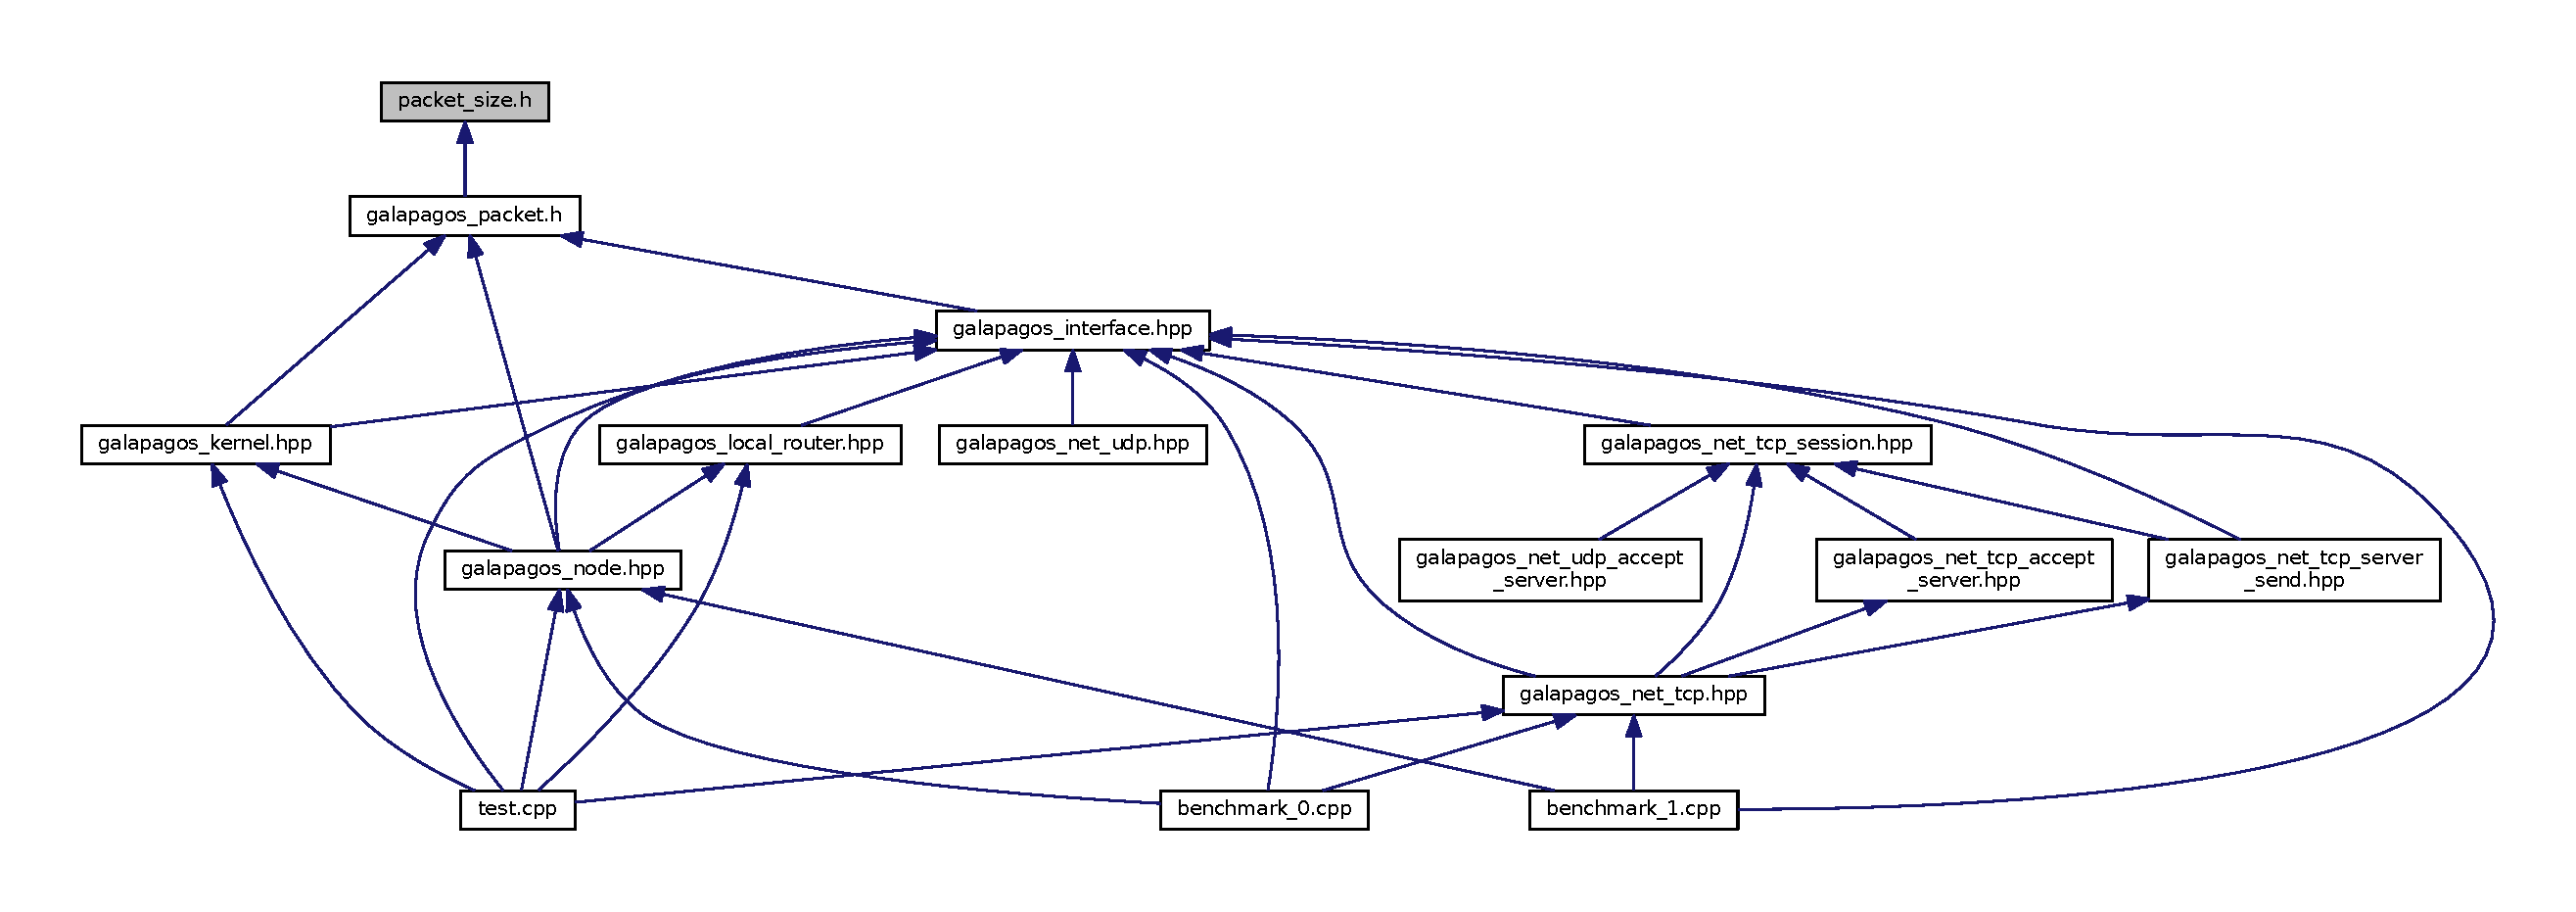
\includegraphics[width=350pt]{packet__size_8h__dep__incl}
\end{center}
\end{figure}
\subsection*{Macros}
\begin{DoxyCompactItemize}
\item 
\#define \hyperlink{packet__size_8h_aaf115bf32d6740657027593bc293743c}{P\+A\+C\+K\+E\+T\+\_\+\+D\+A\+T\+A\+\_\+\+L\+E\+N\+G\+TH}~64
\item 
\#define \hyperlink{packet__size_8h_aee5508cfda1787ded27d89e65f433082}{P\+A\+C\+K\+E\+T\+\_\+\+K\+E\+E\+P\+\_\+\+L\+E\+N\+G\+TH}~8
\item 
\#define \hyperlink{packet__size_8h_aeb4c398a7368938ae6ef9ca06a62a476}{P\+A\+C\+K\+E\+T\+\_\+\+L\+A\+ST}
\item 
\#define \hyperlink{packet__size_8h_af5db3d603be0d574545c417ad0e0520d}{P\+A\+C\+K\+E\+T\+\_\+\+U\+S\+E\+R\+\_\+\+L\+E\+N\+G\+TH}~16
\item 
\#define \hyperlink{packet__size_8h_a5e007ff81bb2779243ac4d9984a00dff}{P\+A\+C\+K\+E\+T\+\_\+\+D\+E\+S\+T\+\_\+\+L\+E\+N\+G\+TH}~8
\end{DoxyCompactItemize}


\subsection{Macro Definition Documentation}
\index{packet\+\_\+size.\+h@{packet\+\_\+size.\+h}!P\+A\+C\+K\+E\+T\+\_\+\+D\+A\+T\+A\+\_\+\+L\+E\+N\+G\+TH@{P\+A\+C\+K\+E\+T\+\_\+\+D\+A\+T\+A\+\_\+\+L\+E\+N\+G\+TH}}
\index{P\+A\+C\+K\+E\+T\+\_\+\+D\+A\+T\+A\+\_\+\+L\+E\+N\+G\+TH@{P\+A\+C\+K\+E\+T\+\_\+\+D\+A\+T\+A\+\_\+\+L\+E\+N\+G\+TH}!packet\+\_\+size.\+h@{packet\+\_\+size.\+h}}
\subsubsection[{\texorpdfstring{P\+A\+C\+K\+E\+T\+\_\+\+D\+A\+T\+A\+\_\+\+L\+E\+N\+G\+TH}{PACKET_DATA_LENGTH}}]{\setlength{\rightskip}{0pt plus 5cm}\#define P\+A\+C\+K\+E\+T\+\_\+\+D\+A\+T\+A\+\_\+\+L\+E\+N\+G\+TH~64}\hypertarget{packet__size_8h_aaf115bf32d6740657027593bc293743c}{}\label{packet__size_8h_aaf115bf32d6740657027593bc293743c}
\index{packet\+\_\+size.\+h@{packet\+\_\+size.\+h}!P\+A\+C\+K\+E\+T\+\_\+\+D\+E\+S\+T\+\_\+\+L\+E\+N\+G\+TH@{P\+A\+C\+K\+E\+T\+\_\+\+D\+E\+S\+T\+\_\+\+L\+E\+N\+G\+TH}}
\index{P\+A\+C\+K\+E\+T\+\_\+\+D\+E\+S\+T\+\_\+\+L\+E\+N\+G\+TH@{P\+A\+C\+K\+E\+T\+\_\+\+D\+E\+S\+T\+\_\+\+L\+E\+N\+G\+TH}!packet\+\_\+size.\+h@{packet\+\_\+size.\+h}}
\subsubsection[{\texorpdfstring{P\+A\+C\+K\+E\+T\+\_\+\+D\+E\+S\+T\+\_\+\+L\+E\+N\+G\+TH}{PACKET_DEST_LENGTH}}]{\setlength{\rightskip}{0pt plus 5cm}\#define P\+A\+C\+K\+E\+T\+\_\+\+D\+E\+S\+T\+\_\+\+L\+E\+N\+G\+TH~8}\hypertarget{packet__size_8h_a5e007ff81bb2779243ac4d9984a00dff}{}\label{packet__size_8h_a5e007ff81bb2779243ac4d9984a00dff}
\index{packet\+\_\+size.\+h@{packet\+\_\+size.\+h}!P\+A\+C\+K\+E\+T\+\_\+\+K\+E\+E\+P\+\_\+\+L\+E\+N\+G\+TH@{P\+A\+C\+K\+E\+T\+\_\+\+K\+E\+E\+P\+\_\+\+L\+E\+N\+G\+TH}}
\index{P\+A\+C\+K\+E\+T\+\_\+\+K\+E\+E\+P\+\_\+\+L\+E\+N\+G\+TH@{P\+A\+C\+K\+E\+T\+\_\+\+K\+E\+E\+P\+\_\+\+L\+E\+N\+G\+TH}!packet\+\_\+size.\+h@{packet\+\_\+size.\+h}}
\subsubsection[{\texorpdfstring{P\+A\+C\+K\+E\+T\+\_\+\+K\+E\+E\+P\+\_\+\+L\+E\+N\+G\+TH}{PACKET_KEEP_LENGTH}}]{\setlength{\rightskip}{0pt plus 5cm}\#define P\+A\+C\+K\+E\+T\+\_\+\+K\+E\+E\+P\+\_\+\+L\+E\+N\+G\+TH~8}\hypertarget{packet__size_8h_aee5508cfda1787ded27d89e65f433082}{}\label{packet__size_8h_aee5508cfda1787ded27d89e65f433082}
\index{packet\+\_\+size.\+h@{packet\+\_\+size.\+h}!P\+A\+C\+K\+E\+T\+\_\+\+L\+A\+ST@{P\+A\+C\+K\+E\+T\+\_\+\+L\+A\+ST}}
\index{P\+A\+C\+K\+E\+T\+\_\+\+L\+A\+ST@{P\+A\+C\+K\+E\+T\+\_\+\+L\+A\+ST}!packet\+\_\+size.\+h@{packet\+\_\+size.\+h}}
\subsubsection[{\texorpdfstring{P\+A\+C\+K\+E\+T\+\_\+\+L\+A\+ST}{PACKET_LAST}}]{\setlength{\rightskip}{0pt plus 5cm}\#define P\+A\+C\+K\+E\+T\+\_\+\+L\+A\+ST}\hypertarget{packet__size_8h_aeb4c398a7368938ae6ef9ca06a62a476}{}\label{packet__size_8h_aeb4c398a7368938ae6ef9ca06a62a476}
\index{packet\+\_\+size.\+h@{packet\+\_\+size.\+h}!P\+A\+C\+K\+E\+T\+\_\+\+U\+S\+E\+R\+\_\+\+L\+E\+N\+G\+TH@{P\+A\+C\+K\+E\+T\+\_\+\+U\+S\+E\+R\+\_\+\+L\+E\+N\+G\+TH}}
\index{P\+A\+C\+K\+E\+T\+\_\+\+U\+S\+E\+R\+\_\+\+L\+E\+N\+G\+TH@{P\+A\+C\+K\+E\+T\+\_\+\+U\+S\+E\+R\+\_\+\+L\+E\+N\+G\+TH}!packet\+\_\+size.\+h@{packet\+\_\+size.\+h}}
\subsubsection[{\texorpdfstring{P\+A\+C\+K\+E\+T\+\_\+\+U\+S\+E\+R\+\_\+\+L\+E\+N\+G\+TH}{PACKET_USER_LENGTH}}]{\setlength{\rightskip}{0pt plus 5cm}\#define P\+A\+C\+K\+E\+T\+\_\+\+U\+S\+E\+R\+\_\+\+L\+E\+N\+G\+TH~16}\hypertarget{packet__size_8h_af5db3d603be0d574545c417ad0e0520d}{}\label{packet__size_8h_af5db3d603be0d574545c417ad0e0520d}

\hypertarget{README_8md}{}\section{R\+E\+A\+D\+M\+E.\+md File Reference}
\label{README_8md}\index{R\+E\+A\+D\+M\+E.\+md@{R\+E\+A\+D\+M\+E.\+md}}

\hypertarget{test_8cpp}{}\section{test.\+cpp File Reference}
\label{test_8cpp}\index{test.\+cpp@{test.\+cpp}}
{\ttfamily \#include \char`\"{}catch.\+hpp\char`\"{}}\\*
{\ttfamily \#include $<$string$>$}\\*
{\ttfamily \#include $<$math.\+h$>$}\\*
{\ttfamily \#include $<$thread$>$}\\*
{\ttfamily \#include $<$chrono$>$}\\*
{\ttfamily \#include \char`\"{}galapagos\+\_\+interface.\+hpp\char`\"{}}\\*
{\ttfamily \#include \char`\"{}galapagos\+\_\+kernel.\+hpp\char`\"{}}\\*
{\ttfamily \#include \char`\"{}galapagos\+\_\+local\+\_\+router.\+hpp\char`\"{}}\\*
{\ttfamily \#include \char`\"{}galapagos\+\_\+external\+\_\+driver.\+hpp\char`\"{}}\\*
{\ttfamily \#include \char`\"{}galapagos\+\_\+net\+\_\+tcp.\+hpp\char`\"{}}\\*
{\ttfamily \#include \char`\"{}galapagos\+\_\+node.\+hpp\char`\"{}}\\*
{\ttfamily \#include \char`\"{}unit\+\_\+tests/kernel.\+h\char`\"{}}\\*
{\ttfamily \#include \char`\"{}unit\+\_\+tests/interface\+\_\+func.\+h\char`\"{}}\\*
{\ttfamily \#include \char`\"{}unit\+\_\+tests/interface\+\_\+perf.\+h\char`\"{}}\\*
{\ttfamily \#include \char`\"{}unit\+\_\+tests/interface\+\_\+splice\+\_\+func.\+h\char`\"{}}\\*
{\ttfamily \#include \char`\"{}unit\+\_\+tests/interface\+\_\+splice\+\_\+perf.\+h\char`\"{}}\\*
{\ttfamily \#include \char`\"{}unit\+\_\+tests/interface\+\_\+trace.\+h\char`\"{}}\\*
{\ttfamily \#include \char`\"{}unit\+\_\+tests/kernel\+\_\+func.\+h\char`\"{}}\\*
{\ttfamily \#include \char`\"{}unit\+\_\+tests/kernel\+\_\+perf.\+h\char`\"{}}\\*
{\ttfamily \#include \char`\"{}unit\+\_\+tests/router\+\_\+kernel\+\_\+func.\+h\char`\"{}}\\*
{\ttfamily \#include \char`\"{}unit\+\_\+tests/router\+\_\+kernel\+\_\+perf.\+h\char`\"{}}\\*
{\ttfamily \#include \char`\"{}unit\+\_\+tests/node\+\_\+func.\+h\char`\"{}}\\*
{\ttfamily \#include \char`\"{}unit\+\_\+tests/node\+\_\+perf.\+h\char`\"{}}\\*
Include dependency graph for test.\+cpp\+:
\nopagebreak
\begin{figure}[H]
\begin{center}
\leavevmode
\includegraphics[width=350pt]{test_8cpp__incl}
\end{center}
\end{figure}
\subsection*{Macros}
\begin{DoxyCompactItemize}
\item 
\#define \hyperlink{test_8cpp_a34b4c3eca7342fbc4cba090d02139902}{C\+A\+T\+C\+H\+\_\+\+C\+O\+N\+F\+I\+G\+\_\+\+R\+U\+N\+N\+ER}
\item 
\#define \hyperlink{test_8cpp_ab3be0641eb76161a48ed528e6eea2ac3}{N\+U\+M\+\_\+\+I\+T\+E\+R\+A\+T\+I\+O\+NS}~100000
\end{DoxyCompactItemize}
\subsection*{Typedefs}
\begin{DoxyCompactItemize}
\item 
typedef ap\+\_\+uint$<$ 64 $>$ \hyperlink{test_8cpp_a0658ceffa730c765d449bb3d21871b5f}{T}
\end{DoxyCompactItemize}
\subsection*{Functions}
\begin{DoxyCompactItemize}
\item 
std\+::string \hyperlink{test_8cpp_ad6c70ba8571527f1543822ce71b9a109}{my\+\_\+address} (\char`\"{}10.\+0.\+0.\+1\char`\"{})
\item 
std\+::string \hyperlink{test_8cpp_a26080a439da4e3dd098bb6146f946bce}{remote\+\_\+address} (\char`\"{}10.\+0.\+0.\+2\char`\"{})
\item 
void \hyperlink{test_8cpp_a952c103146dc9b79782931ba3fa131f1}{generate\+\_\+flit} (int iterations, int size, int id, int dest, \hyperlink{galapagos__interface_8hpp_af5070d0f7a016a7cd5677cdf2e30ac63}{galapagos\+\_\+interface} $\ast$out)
\item 
void \hyperlink{test_8cpp_a54f037e7a8d79a8557a33713c97c3ed8}{generate\+\_\+packet} (int iterations, int size, int id, int dest, \hyperlink{galapagos__interface_8hpp_af5070d0f7a016a7cd5677cdf2e30ac63}{galapagos\+\_\+interface} $\ast$out)
\item 
void \hyperlink{test_8cpp_a79daffd29405a76f0c0676b577e2843d}{generate\+\_\+packet} (char $\ast$mem, int iterations, int size, int id, int dest, \hyperlink{galapagos__interface_8hpp_af5070d0f7a016a7cd5677cdf2e30ac63}{galapagos\+\_\+interface} $\ast$out)
\item 
void \hyperlink{test_8cpp_a83fe9f71488e293cfe12208b9a4b082a}{generate\+\_\+packet} (std\+::vector$<$ ap\+\_\+uint$<$ 64 $>$ $>$ $\ast$vec, int iterations, int size, int id, int dest, \hyperlink{galapagos__interface_8hpp_af5070d0f7a016a7cd5677cdf2e30ac63}{galapagos\+\_\+interface} $\ast$out)
\item 
void \hyperlink{test_8cpp_ab58f1ce436d790a26a5c52969cb832aa}{receive\+\_\+flit\+\_\+perf} (int iterations, int size, \hyperlink{galapagos__interface_8hpp_af5070d0f7a016a7cd5677cdf2e30ac63}{galapagos\+\_\+interface} $\ast$in)
\item 
void \hyperlink{test_8cpp_affc065c5706e3d2766ff79d86064eba6}{receive\+\_\+packet\+\_\+perf} (int iterations, int size, \hyperlink{galapagos__interface_8hpp_af5070d0f7a016a7cd5677cdf2e30ac63}{galapagos\+\_\+interface} $\ast$in)
\item 
void \hyperlink{test_8cpp_a9333d960ef4e8263bada8171199335c9}{kern\+\_\+generate\+\_\+flit} (short id, \hyperlink{galapagos__interface_8hpp_af5070d0f7a016a7cd5677cdf2e30ac63}{galapagos\+\_\+interface} $\ast$in, \hyperlink{galapagos__interface_8hpp_af5070d0f7a016a7cd5677cdf2e30ac63}{galapagos\+\_\+interface} $\ast$out)
\item 
void \hyperlink{test_8cpp_a91143d0f19f313fe8660e05907e37536}{kern\+\_\+generate\+\_\+packet} (short id, \hyperlink{galapagos__interface_8hpp_af5070d0f7a016a7cd5677cdf2e30ac63}{galapagos\+\_\+interface} $\ast$in, \hyperlink{galapagos__interface_8hpp_af5070d0f7a016a7cd5677cdf2e30ac63}{galapagos\+\_\+interface} $\ast$out)
\item 
void \hyperlink{test_8cpp_a80c90cf9b607ea4fc6e2512983b491ea}{kern\+\_\+output\+\_\+flit\+\_\+verify} (short id, \hyperlink{galapagos__interface_8hpp_af5070d0f7a016a7cd5677cdf2e30ac63}{galapagos\+\_\+interface} $\ast$in, \hyperlink{galapagos__interface_8hpp_af5070d0f7a016a7cd5677cdf2e30ac63}{galapagos\+\_\+interface} $\ast$out)
\item 
void \hyperlink{test_8cpp_a1a08eeff3ffa31aa5194be1e6a89c0ab}{kern\+\_\+output\+\_\+packet\+\_\+verify} (short id, \hyperlink{galapagos__interface_8hpp_af5070d0f7a016a7cd5677cdf2e30ac63}{galapagos\+\_\+interface} $\ast$in, \hyperlink{galapagos__interface_8hpp_af5070d0f7a016a7cd5677cdf2e30ac63}{galapagos\+\_\+interface} $\ast$out)
\item 
void \hyperlink{test_8cpp_a4aba7a81f4edf73f72b47c1764d2366d}{kern\+\_\+output\+\_\+flit\+\_\+perf} (short id, \hyperlink{galapagos__interface_8hpp_af5070d0f7a016a7cd5677cdf2e30ac63}{galapagos\+\_\+interface} $\ast$in, \hyperlink{galapagos__interface_8hpp_af5070d0f7a016a7cd5677cdf2e30ac63}{galapagos\+\_\+interface} $\ast$out)
\item 
void \hyperlink{test_8cpp_aadf5d569e1e0feb11bb6b6b4d04336c0}{kern\+\_\+output\+\_\+packet\+\_\+perf} (short id, \hyperlink{galapagos__interface_8hpp_af5070d0f7a016a7cd5677cdf2e30ac63}{galapagos\+\_\+interface} $\ast$in, \hyperlink{galapagos__interface_8hpp_af5070d0f7a016a7cd5677cdf2e30ac63}{galapagos\+\_\+interface} $\ast$out)
\item 
void \hyperlink{test_8cpp_a11e7c13bf1c721efd6473e2d16b0b264}{axis\+\_\+fifo} (\hyperlink{galapagos__interface_8hpp_af5070d0f7a016a7cd5677cdf2e30ac63}{galapagos\+\_\+interface} $\ast$s\+\_\+axis, \hyperlink{galapagos__interface_8hpp_af5070d0f7a016a7cd5677cdf2e30ac63}{galapagos\+\_\+interface} $\ast$m\+\_\+axis, int count)
\item 
void \hyperlink{test_8cpp_a3a6c4d524ee19ccec113ae38b192d84d}{send\+\_\+single\+\_\+flit} (short id, \hyperlink{galapagos__interface_8hpp_af5070d0f7a016a7cd5677cdf2e30ac63}{galapagos\+\_\+interface} $\ast$in, \hyperlink{galapagos__interface_8hpp_af5070d0f7a016a7cd5677cdf2e30ac63}{galapagos\+\_\+interface} $\ast$out)
\item 
void \hyperlink{test_8cpp_ac861395ca6cdcc55f4d3958f4747a5e6}{send\+\_\+single\+\_\+packet} (short id, \hyperlink{galapagos__interface_8hpp_af5070d0f7a016a7cd5677cdf2e30ac63}{galapagos\+\_\+interface} $\ast$in, \hyperlink{galapagos__interface_8hpp_af5070d0f7a016a7cd5677cdf2e30ac63}{galapagos\+\_\+interface} $\ast$out)
\item 
void \hyperlink{test_8cpp_a6104170a04da9a4d3a02507f626a87db}{recv\+\_\+single\+\_\+flit} (short id, \hyperlink{galapagos__interface_8hpp_af5070d0f7a016a7cd5677cdf2e30ac63}{galapagos\+\_\+interface} $\ast$in, \hyperlink{galapagos__interface_8hpp_af5070d0f7a016a7cd5677cdf2e30ac63}{galapagos\+\_\+interface} $\ast$out)
\item 
void \hyperlink{test_8cpp_a881e8d624ad60d92bd851d0edd13115c}{recv\+\_\+single\+\_\+packet} (short id, \hyperlink{galapagos__interface_8hpp_af5070d0f7a016a7cd5677cdf2e30ac63}{galapagos\+\_\+interface} $\ast$in, \hyperlink{galapagos__interface_8hpp_af5070d0f7a016a7cd5677cdf2e30ac63}{galapagos\+\_\+interface} $\ast$out)
\item 
void \hyperlink{test_8cpp_a8ca88d3e17110eb3b7d601ccd1ad1b83}{kern\+\_\+flit\+\_\+loopback\+\_\+perf} (short id, \hyperlink{galapagos__interface_8hpp_af5070d0f7a016a7cd5677cdf2e30ac63}{galapagos\+\_\+interface} $\ast$in, \hyperlink{galapagos__interface_8hpp_af5070d0f7a016a7cd5677cdf2e30ac63}{galapagos\+\_\+interface} $\ast$out)
\item 
void \hyperlink{test_8cpp_a19d34c353699396428b4f5b55e39d803}{kern\+\_\+flit\+\_\+loopback\+\_\+verify} (short id, \hyperlink{galapagos__interface_8hpp_af5070d0f7a016a7cd5677cdf2e30ac63}{galapagos\+\_\+interface} $\ast$in, \hyperlink{galapagos__interface_8hpp_af5070d0f7a016a7cd5677cdf2e30ac63}{galapagos\+\_\+interface} $\ast$out)
\item 
void \hyperlink{test_8cpp_a7eac1551dbf19f63635523f230364dd2}{kern\+\_\+packet\+\_\+loopback\+\_\+perf} (short id, \hyperlink{galapagos__interface_8hpp_af5070d0f7a016a7cd5677cdf2e30ac63}{galapagos\+\_\+interface} $\ast$in, \hyperlink{galapagos__interface_8hpp_af5070d0f7a016a7cd5677cdf2e30ac63}{galapagos\+\_\+interface} $\ast$out)
\item 
void \hyperlink{test_8cpp_a06f045135a0ee0b574120cab307693c8}{kern\+\_\+packet\+\_\+loopback\+\_\+verify} (short id, \hyperlink{galapagos__interface_8hpp_af5070d0f7a016a7cd5677cdf2e30ac63}{galapagos\+\_\+interface} $\ast$in, \hyperlink{galapagos__interface_8hpp_af5070d0f7a016a7cd5677cdf2e30ac63}{galapagos\+\_\+interface} $\ast$out)
\item 
void \hyperlink{test_8cpp_af5cc631d8fae454651ecb0c5fbf23047}{kern\+\_\+generate\+\_\+output\+\_\+flit\+\_\+verify} (short id, \hyperlink{galapagos__interface_8hpp_af5070d0f7a016a7cd5677cdf2e30ac63}{galapagos\+\_\+interface} $\ast$in, \hyperlink{galapagos__interface_8hpp_af5070d0f7a016a7cd5677cdf2e30ac63}{galapagos\+\_\+interface} $\ast$out)
\item 
void \hyperlink{test_8cpp_a2199bc9b3b277f26da99d4c55124be01}{kern\+\_\+generate\+\_\+output\+\_\+packet\+\_\+verify} (short id, \hyperlink{galapagos__interface_8hpp_af5070d0f7a016a7cd5677cdf2e30ac63}{galapagos\+\_\+interface} $\ast$in, \hyperlink{galapagos__interface_8hpp_af5070d0f7a016a7cd5677cdf2e30ac63}{galapagos\+\_\+interface} $\ast$out)
\item 
void \hyperlink{test_8cpp_a2218d858bef70dd73ec06bd5e6963406}{kern\+\_\+generate\+\_\+output\+\_\+flit\+\_\+perf} (short id, \hyperlink{galapagos__interface_8hpp_af5070d0f7a016a7cd5677cdf2e30ac63}{galapagos\+\_\+interface} $\ast$in, \hyperlink{galapagos__interface_8hpp_af5070d0f7a016a7cd5677cdf2e30ac63}{galapagos\+\_\+interface} $\ast$out)
\item 
void \hyperlink{test_8cpp_addbaf4f92b1d1dd46e7df9875ac997d2}{kern\+\_\+generate\+\_\+output\+\_\+packet\+\_\+perf} (short id, \hyperlink{galapagos__interface_8hpp_af5070d0f7a016a7cd5677cdf2e30ac63}{galapagos\+\_\+interface} $\ast$in, \hyperlink{galapagos__interface_8hpp_af5070d0f7a016a7cd5677cdf2e30ac63}{galapagos\+\_\+interface} $\ast$out)
\item 
int \hyperlink{test_8cpp_a0ddf1224851353fc92bfbff6f499fa97}{main} (int argc, char $\ast$argv\mbox{[}$\,$\mbox{]})
\end{DoxyCompactItemize}
\subsection*{Variables}
\begin{DoxyCompactItemize}
\item 
std\+::chrono\+::time\+\_\+point$<$ std\+::chrono\+::high\+\_\+resolution\+\_\+clock $>$ \hyperlink{test_8cpp_a46dea58f2d527f376090214bd5c3233d}{start}
\item 
std\+::chrono\+::time\+\_\+point$<$ std\+::chrono\+::high\+\_\+resolution\+\_\+clock $>$ \hyperlink{test_8cpp_ace54cb99b52f35f3a98f99e2a75dd5ad}{end}
\end{DoxyCompactItemize}


\subsection{Macro Definition Documentation}
\index{test.\+cpp@{test.\+cpp}!C\+A\+T\+C\+H\+\_\+\+C\+O\+N\+F\+I\+G\+\_\+\+R\+U\+N\+N\+ER@{C\+A\+T\+C\+H\+\_\+\+C\+O\+N\+F\+I\+G\+\_\+\+R\+U\+N\+N\+ER}}
\index{C\+A\+T\+C\+H\+\_\+\+C\+O\+N\+F\+I\+G\+\_\+\+R\+U\+N\+N\+ER@{C\+A\+T\+C\+H\+\_\+\+C\+O\+N\+F\+I\+G\+\_\+\+R\+U\+N\+N\+ER}!test.\+cpp@{test.\+cpp}}
\subsubsection[{\texorpdfstring{C\+A\+T\+C\+H\+\_\+\+C\+O\+N\+F\+I\+G\+\_\+\+R\+U\+N\+N\+ER}{CATCH_CONFIG_RUNNER}}]{\setlength{\rightskip}{0pt plus 5cm}\#define C\+A\+T\+C\+H\+\_\+\+C\+O\+N\+F\+I\+G\+\_\+\+R\+U\+N\+N\+ER}\hypertarget{test_8cpp_a34b4c3eca7342fbc4cba090d02139902}{}\label{test_8cpp_a34b4c3eca7342fbc4cba090d02139902}
\index{test.\+cpp@{test.\+cpp}!N\+U\+M\+\_\+\+I\+T\+E\+R\+A\+T\+I\+O\+NS@{N\+U\+M\+\_\+\+I\+T\+E\+R\+A\+T\+I\+O\+NS}}
\index{N\+U\+M\+\_\+\+I\+T\+E\+R\+A\+T\+I\+O\+NS@{N\+U\+M\+\_\+\+I\+T\+E\+R\+A\+T\+I\+O\+NS}!test.\+cpp@{test.\+cpp}}
\subsubsection[{\texorpdfstring{N\+U\+M\+\_\+\+I\+T\+E\+R\+A\+T\+I\+O\+NS}{NUM_ITERATIONS}}]{\setlength{\rightskip}{0pt plus 5cm}\#define N\+U\+M\+\_\+\+I\+T\+E\+R\+A\+T\+I\+O\+NS~100000}\hypertarget{test_8cpp_ab3be0641eb76161a48ed528e6eea2ac3}{}\label{test_8cpp_ab3be0641eb76161a48ed528e6eea2ac3}


\subsection{Typedef Documentation}
\index{test.\+cpp@{test.\+cpp}!T@{T}}
\index{T@{T}!test.\+cpp@{test.\+cpp}}
\subsubsection[{\texorpdfstring{T}{T}}]{\setlength{\rightskip}{0pt plus 5cm}typedef ap\+\_\+uint$<$64$>$ {\bf T}}\hypertarget{test_8cpp_a0658ceffa730c765d449bb3d21871b5f}{}\label{test_8cpp_a0658ceffa730c765d449bb3d21871b5f}


\subsection{Function Documentation}
\index{test.\+cpp@{test.\+cpp}!axis\+\_\+fifo@{axis\+\_\+fifo}}
\index{axis\+\_\+fifo@{axis\+\_\+fifo}!test.\+cpp@{test.\+cpp}}
\subsubsection[{\texorpdfstring{axis\+\_\+fifo(galapagos\+\_\+interface $\ast$s\+\_\+axis, galapagos\+\_\+interface $\ast$m\+\_\+axis, int count)}{axis_fifo(galapagos_interface *s_axis, galapagos_interface *m_axis, int count)}}]{\setlength{\rightskip}{0pt plus 5cm}void axis\+\_\+fifo (
\begin{DoxyParamCaption}
\item[{{\bf galapagos\+\_\+interface} $\ast$}]{s\+\_\+axis, }
\item[{{\bf galapagos\+\_\+interface} $\ast$}]{m\+\_\+axis, }
\item[{int}]{count}
\end{DoxyParamCaption}
)}\hypertarget{test_8cpp_a11e7c13bf1c721efd6473e2d16b0b264}{}\label{test_8cpp_a11e7c13bf1c721efd6473e2d16b0b264}
\index{test.\+cpp@{test.\+cpp}!generate\+\_\+flit@{generate\+\_\+flit}}
\index{generate\+\_\+flit@{generate\+\_\+flit}!test.\+cpp@{test.\+cpp}}
\subsubsection[{\texorpdfstring{generate\+\_\+flit(int iterations, int size, int id, int dest, galapagos\+\_\+interface $\ast$out)}{generate_flit(int iterations, int size, int id, int dest, galapagos_interface *out)}}]{\setlength{\rightskip}{0pt plus 5cm}void generate\+\_\+flit (
\begin{DoxyParamCaption}
\item[{int}]{iterations, }
\item[{int}]{size, }
\item[{int}]{id, }
\item[{int}]{dest, }
\item[{{\bf galapagos\+\_\+interface} $\ast$}]{out}
\end{DoxyParamCaption}
)}\hypertarget{test_8cpp_a952c103146dc9b79782931ba3fa131f1}{}\label{test_8cpp_a952c103146dc9b79782931ba3fa131f1}
\index{test.\+cpp@{test.\+cpp}!generate\+\_\+packet@{generate\+\_\+packet}}
\index{generate\+\_\+packet@{generate\+\_\+packet}!test.\+cpp@{test.\+cpp}}
\subsubsection[{\texorpdfstring{generate\+\_\+packet(int iterations, int size, int id, int dest, galapagos\+\_\+interface $\ast$out)}{generate_packet(int iterations, int size, int id, int dest, galapagos_interface *out)}}]{\setlength{\rightskip}{0pt plus 5cm}void generate\+\_\+packet (
\begin{DoxyParamCaption}
\item[{int}]{iterations, }
\item[{int}]{size, }
\item[{int}]{id, }
\item[{int}]{dest, }
\item[{{\bf galapagos\+\_\+interface} $\ast$}]{out}
\end{DoxyParamCaption}
)}\hypertarget{test_8cpp_a54f037e7a8d79a8557a33713c97c3ed8}{}\label{test_8cpp_a54f037e7a8d79a8557a33713c97c3ed8}
\index{test.\+cpp@{test.\+cpp}!generate\+\_\+packet@{generate\+\_\+packet}}
\index{generate\+\_\+packet@{generate\+\_\+packet}!test.\+cpp@{test.\+cpp}}
\subsubsection[{\texorpdfstring{generate\+\_\+packet(char $\ast$mem, int iterations, int size, int id, int dest, galapagos\+\_\+interface $\ast$out)}{generate_packet(char *mem, int iterations, int size, int id, int dest, galapagos_interface *out)}}]{\setlength{\rightskip}{0pt plus 5cm}void generate\+\_\+packet (
\begin{DoxyParamCaption}
\item[{char $\ast$}]{mem, }
\item[{int}]{iterations, }
\item[{int}]{size, }
\item[{int}]{id, }
\item[{int}]{dest, }
\item[{{\bf galapagos\+\_\+interface} $\ast$}]{out}
\end{DoxyParamCaption}
)}\hypertarget{test_8cpp_a79daffd29405a76f0c0676b577e2843d}{}\label{test_8cpp_a79daffd29405a76f0c0676b577e2843d}
\index{test.\+cpp@{test.\+cpp}!generate\+\_\+packet@{generate\+\_\+packet}}
\index{generate\+\_\+packet@{generate\+\_\+packet}!test.\+cpp@{test.\+cpp}}
\subsubsection[{\texorpdfstring{generate\+\_\+packet(std\+::vector$<$ ap\+\_\+uint$<$ 64 $>$ $>$ $\ast$vec, int iterations, int size, int id, int dest, galapagos\+\_\+interface $\ast$out)}{generate_packet(std::vector< ap_uint< 64 > > *vec, int iterations, int size, int id, int dest, galapagos_interface *out)}}]{\setlength{\rightskip}{0pt plus 5cm}void generate\+\_\+packet (
\begin{DoxyParamCaption}
\item[{std\+::vector$<$ ap\+\_\+uint$<$ 64 $>$ $>$ $\ast$}]{vec, }
\item[{int}]{iterations, }
\item[{int}]{size, }
\item[{int}]{id, }
\item[{int}]{dest, }
\item[{{\bf galapagos\+\_\+interface} $\ast$}]{out}
\end{DoxyParamCaption}
)}\hypertarget{test_8cpp_a83fe9f71488e293cfe12208b9a4b082a}{}\label{test_8cpp_a83fe9f71488e293cfe12208b9a4b082a}
\index{test.\+cpp@{test.\+cpp}!kern\+\_\+flit\+\_\+loopback\+\_\+perf@{kern\+\_\+flit\+\_\+loopback\+\_\+perf}}
\index{kern\+\_\+flit\+\_\+loopback\+\_\+perf@{kern\+\_\+flit\+\_\+loopback\+\_\+perf}!test.\+cpp@{test.\+cpp}}
\subsubsection[{\texorpdfstring{kern\+\_\+flit\+\_\+loopback\+\_\+perf(short id, galapagos\+\_\+interface $\ast$in, galapagos\+\_\+interface $\ast$out)}{kern_flit_loopback_perf(short id, galapagos_interface *in, galapagos_interface *out)}}]{\setlength{\rightskip}{0pt plus 5cm}void kern\+\_\+flit\+\_\+loopback\+\_\+perf (
\begin{DoxyParamCaption}
\item[{short}]{id, }
\item[{{\bf galapagos\+\_\+interface} $\ast$}]{in, }
\item[{{\bf galapagos\+\_\+interface} $\ast$}]{out}
\end{DoxyParamCaption}
)}\hypertarget{test_8cpp_a8ca88d3e17110eb3b7d601ccd1ad1b83}{}\label{test_8cpp_a8ca88d3e17110eb3b7d601ccd1ad1b83}
\index{test.\+cpp@{test.\+cpp}!kern\+\_\+flit\+\_\+loopback\+\_\+verify@{kern\+\_\+flit\+\_\+loopback\+\_\+verify}}
\index{kern\+\_\+flit\+\_\+loopback\+\_\+verify@{kern\+\_\+flit\+\_\+loopback\+\_\+verify}!test.\+cpp@{test.\+cpp}}
\subsubsection[{\texorpdfstring{kern\+\_\+flit\+\_\+loopback\+\_\+verify(short id, galapagos\+\_\+interface $\ast$in, galapagos\+\_\+interface $\ast$out)}{kern_flit_loopback_verify(short id, galapagos_interface *in, galapagos_interface *out)}}]{\setlength{\rightskip}{0pt plus 5cm}void kern\+\_\+flit\+\_\+loopback\+\_\+verify (
\begin{DoxyParamCaption}
\item[{short}]{id, }
\item[{{\bf galapagos\+\_\+interface} $\ast$}]{in, }
\item[{{\bf galapagos\+\_\+interface} $\ast$}]{out}
\end{DoxyParamCaption}
)}\hypertarget{test_8cpp_a19d34c353699396428b4f5b55e39d803}{}\label{test_8cpp_a19d34c353699396428b4f5b55e39d803}
\index{test.\+cpp@{test.\+cpp}!kern\+\_\+generate\+\_\+flit@{kern\+\_\+generate\+\_\+flit}}
\index{kern\+\_\+generate\+\_\+flit@{kern\+\_\+generate\+\_\+flit}!test.\+cpp@{test.\+cpp}}
\subsubsection[{\texorpdfstring{kern\+\_\+generate\+\_\+flit(short id, galapagos\+\_\+interface $\ast$in, galapagos\+\_\+interface $\ast$out)}{kern_generate_flit(short id, galapagos_interface *in, galapagos_interface *out)}}]{\setlength{\rightskip}{0pt plus 5cm}void kern\+\_\+generate\+\_\+flit (
\begin{DoxyParamCaption}
\item[{short}]{id, }
\item[{{\bf galapagos\+\_\+interface} $\ast$}]{in, }
\item[{{\bf galapagos\+\_\+interface} $\ast$}]{out}
\end{DoxyParamCaption}
)}\hypertarget{test_8cpp_a9333d960ef4e8263bada8171199335c9}{}\label{test_8cpp_a9333d960ef4e8263bada8171199335c9}
\index{test.\+cpp@{test.\+cpp}!kern\+\_\+generate\+\_\+output\+\_\+flit\+\_\+perf@{kern\+\_\+generate\+\_\+output\+\_\+flit\+\_\+perf}}
\index{kern\+\_\+generate\+\_\+output\+\_\+flit\+\_\+perf@{kern\+\_\+generate\+\_\+output\+\_\+flit\+\_\+perf}!test.\+cpp@{test.\+cpp}}
\subsubsection[{\texorpdfstring{kern\+\_\+generate\+\_\+output\+\_\+flit\+\_\+perf(short id, galapagos\+\_\+interface $\ast$in, galapagos\+\_\+interface $\ast$out)}{kern_generate_output_flit_perf(short id, galapagos_interface *in, galapagos_interface *out)}}]{\setlength{\rightskip}{0pt plus 5cm}void kern\+\_\+generate\+\_\+output\+\_\+flit\+\_\+perf (
\begin{DoxyParamCaption}
\item[{short}]{id, }
\item[{{\bf galapagos\+\_\+interface} $\ast$}]{in, }
\item[{{\bf galapagos\+\_\+interface} $\ast$}]{out}
\end{DoxyParamCaption}
)}\hypertarget{test_8cpp_a2218d858bef70dd73ec06bd5e6963406}{}\label{test_8cpp_a2218d858bef70dd73ec06bd5e6963406}
\index{test.\+cpp@{test.\+cpp}!kern\+\_\+generate\+\_\+output\+\_\+flit\+\_\+verify@{kern\+\_\+generate\+\_\+output\+\_\+flit\+\_\+verify}}
\index{kern\+\_\+generate\+\_\+output\+\_\+flit\+\_\+verify@{kern\+\_\+generate\+\_\+output\+\_\+flit\+\_\+verify}!test.\+cpp@{test.\+cpp}}
\subsubsection[{\texorpdfstring{kern\+\_\+generate\+\_\+output\+\_\+flit\+\_\+verify(short id, galapagos\+\_\+interface $\ast$in, galapagos\+\_\+interface $\ast$out)}{kern_generate_output_flit_verify(short id, galapagos_interface *in, galapagos_interface *out)}}]{\setlength{\rightskip}{0pt plus 5cm}void kern\+\_\+generate\+\_\+output\+\_\+flit\+\_\+verify (
\begin{DoxyParamCaption}
\item[{short}]{id, }
\item[{{\bf galapagos\+\_\+interface} $\ast$}]{in, }
\item[{{\bf galapagos\+\_\+interface} $\ast$}]{out}
\end{DoxyParamCaption}
)}\hypertarget{test_8cpp_af5cc631d8fae454651ecb0c5fbf23047}{}\label{test_8cpp_af5cc631d8fae454651ecb0c5fbf23047}
\index{test.\+cpp@{test.\+cpp}!kern\+\_\+generate\+\_\+output\+\_\+packet\+\_\+perf@{kern\+\_\+generate\+\_\+output\+\_\+packet\+\_\+perf}}
\index{kern\+\_\+generate\+\_\+output\+\_\+packet\+\_\+perf@{kern\+\_\+generate\+\_\+output\+\_\+packet\+\_\+perf}!test.\+cpp@{test.\+cpp}}
\subsubsection[{\texorpdfstring{kern\+\_\+generate\+\_\+output\+\_\+packet\+\_\+perf(short id, galapagos\+\_\+interface $\ast$in, galapagos\+\_\+interface $\ast$out)}{kern_generate_output_packet_perf(short id, galapagos_interface *in, galapagos_interface *out)}}]{\setlength{\rightskip}{0pt plus 5cm}void kern\+\_\+generate\+\_\+output\+\_\+packet\+\_\+perf (
\begin{DoxyParamCaption}
\item[{short}]{id, }
\item[{{\bf galapagos\+\_\+interface} $\ast$}]{in, }
\item[{{\bf galapagos\+\_\+interface} $\ast$}]{out}
\end{DoxyParamCaption}
)}\hypertarget{test_8cpp_addbaf4f92b1d1dd46e7df9875ac997d2}{}\label{test_8cpp_addbaf4f92b1d1dd46e7df9875ac997d2}
\index{test.\+cpp@{test.\+cpp}!kern\+\_\+generate\+\_\+output\+\_\+packet\+\_\+verify@{kern\+\_\+generate\+\_\+output\+\_\+packet\+\_\+verify}}
\index{kern\+\_\+generate\+\_\+output\+\_\+packet\+\_\+verify@{kern\+\_\+generate\+\_\+output\+\_\+packet\+\_\+verify}!test.\+cpp@{test.\+cpp}}
\subsubsection[{\texorpdfstring{kern\+\_\+generate\+\_\+output\+\_\+packet\+\_\+verify(short id, galapagos\+\_\+interface $\ast$in, galapagos\+\_\+interface $\ast$out)}{kern_generate_output_packet_verify(short id, galapagos_interface *in, galapagos_interface *out)}}]{\setlength{\rightskip}{0pt plus 5cm}void kern\+\_\+generate\+\_\+output\+\_\+packet\+\_\+verify (
\begin{DoxyParamCaption}
\item[{short}]{id, }
\item[{{\bf galapagos\+\_\+interface} $\ast$}]{in, }
\item[{{\bf galapagos\+\_\+interface} $\ast$}]{out}
\end{DoxyParamCaption}
)}\hypertarget{test_8cpp_a2199bc9b3b277f26da99d4c55124be01}{}\label{test_8cpp_a2199bc9b3b277f26da99d4c55124be01}
\index{test.\+cpp@{test.\+cpp}!kern\+\_\+generate\+\_\+packet@{kern\+\_\+generate\+\_\+packet}}
\index{kern\+\_\+generate\+\_\+packet@{kern\+\_\+generate\+\_\+packet}!test.\+cpp@{test.\+cpp}}
\subsubsection[{\texorpdfstring{kern\+\_\+generate\+\_\+packet(short id, galapagos\+\_\+interface $\ast$in, galapagos\+\_\+interface $\ast$out)}{kern_generate_packet(short id, galapagos_interface *in, galapagos_interface *out)}}]{\setlength{\rightskip}{0pt plus 5cm}void kern\+\_\+generate\+\_\+packet (
\begin{DoxyParamCaption}
\item[{short}]{id, }
\item[{{\bf galapagos\+\_\+interface} $\ast$}]{in, }
\item[{{\bf galapagos\+\_\+interface} $\ast$}]{out}
\end{DoxyParamCaption}
)}\hypertarget{test_8cpp_a91143d0f19f313fe8660e05907e37536}{}\label{test_8cpp_a91143d0f19f313fe8660e05907e37536}
\index{test.\+cpp@{test.\+cpp}!kern\+\_\+output\+\_\+flit\+\_\+perf@{kern\+\_\+output\+\_\+flit\+\_\+perf}}
\index{kern\+\_\+output\+\_\+flit\+\_\+perf@{kern\+\_\+output\+\_\+flit\+\_\+perf}!test.\+cpp@{test.\+cpp}}
\subsubsection[{\texorpdfstring{kern\+\_\+output\+\_\+flit\+\_\+perf(short id, galapagos\+\_\+interface $\ast$in, galapagos\+\_\+interface $\ast$out)}{kern_output_flit_perf(short id, galapagos_interface *in, galapagos_interface *out)}}]{\setlength{\rightskip}{0pt plus 5cm}void kern\+\_\+output\+\_\+flit\+\_\+perf (
\begin{DoxyParamCaption}
\item[{short}]{id, }
\item[{{\bf galapagos\+\_\+interface} $\ast$}]{in, }
\item[{{\bf galapagos\+\_\+interface} $\ast$}]{out}
\end{DoxyParamCaption}
)}\hypertarget{test_8cpp_a4aba7a81f4edf73f72b47c1764d2366d}{}\label{test_8cpp_a4aba7a81f4edf73f72b47c1764d2366d}
\index{test.\+cpp@{test.\+cpp}!kern\+\_\+output\+\_\+flit\+\_\+verify@{kern\+\_\+output\+\_\+flit\+\_\+verify}}
\index{kern\+\_\+output\+\_\+flit\+\_\+verify@{kern\+\_\+output\+\_\+flit\+\_\+verify}!test.\+cpp@{test.\+cpp}}
\subsubsection[{\texorpdfstring{kern\+\_\+output\+\_\+flit\+\_\+verify(short id, galapagos\+\_\+interface $\ast$in, galapagos\+\_\+interface $\ast$out)}{kern_output_flit_verify(short id, galapagos_interface *in, galapagos_interface *out)}}]{\setlength{\rightskip}{0pt plus 5cm}void kern\+\_\+output\+\_\+flit\+\_\+verify (
\begin{DoxyParamCaption}
\item[{short}]{id, }
\item[{{\bf galapagos\+\_\+interface} $\ast$}]{in, }
\item[{{\bf galapagos\+\_\+interface} $\ast$}]{out}
\end{DoxyParamCaption}
)}\hypertarget{test_8cpp_a80c90cf9b607ea4fc6e2512983b491ea}{}\label{test_8cpp_a80c90cf9b607ea4fc6e2512983b491ea}
\index{test.\+cpp@{test.\+cpp}!kern\+\_\+output\+\_\+packet\+\_\+perf@{kern\+\_\+output\+\_\+packet\+\_\+perf}}
\index{kern\+\_\+output\+\_\+packet\+\_\+perf@{kern\+\_\+output\+\_\+packet\+\_\+perf}!test.\+cpp@{test.\+cpp}}
\subsubsection[{\texorpdfstring{kern\+\_\+output\+\_\+packet\+\_\+perf(short id, galapagos\+\_\+interface $\ast$in, galapagos\+\_\+interface $\ast$out)}{kern_output_packet_perf(short id, galapagos_interface *in, galapagos_interface *out)}}]{\setlength{\rightskip}{0pt plus 5cm}void kern\+\_\+output\+\_\+packet\+\_\+perf (
\begin{DoxyParamCaption}
\item[{short}]{id, }
\item[{{\bf galapagos\+\_\+interface} $\ast$}]{in, }
\item[{{\bf galapagos\+\_\+interface} $\ast$}]{out}
\end{DoxyParamCaption}
)}\hypertarget{test_8cpp_aadf5d569e1e0feb11bb6b6b4d04336c0}{}\label{test_8cpp_aadf5d569e1e0feb11bb6b6b4d04336c0}
\index{test.\+cpp@{test.\+cpp}!kern\+\_\+output\+\_\+packet\+\_\+verify@{kern\+\_\+output\+\_\+packet\+\_\+verify}}
\index{kern\+\_\+output\+\_\+packet\+\_\+verify@{kern\+\_\+output\+\_\+packet\+\_\+verify}!test.\+cpp@{test.\+cpp}}
\subsubsection[{\texorpdfstring{kern\+\_\+output\+\_\+packet\+\_\+verify(short id, galapagos\+\_\+interface $\ast$in, galapagos\+\_\+interface $\ast$out)}{kern_output_packet_verify(short id, galapagos_interface *in, galapagos_interface *out)}}]{\setlength{\rightskip}{0pt plus 5cm}void kern\+\_\+output\+\_\+packet\+\_\+verify (
\begin{DoxyParamCaption}
\item[{short}]{id, }
\item[{{\bf galapagos\+\_\+interface} $\ast$}]{in, }
\item[{{\bf galapagos\+\_\+interface} $\ast$}]{out}
\end{DoxyParamCaption}
)}\hypertarget{test_8cpp_a1a08eeff3ffa31aa5194be1e6a89c0ab}{}\label{test_8cpp_a1a08eeff3ffa31aa5194be1e6a89c0ab}
\index{test.\+cpp@{test.\+cpp}!kern\+\_\+packet\+\_\+loopback\+\_\+perf@{kern\+\_\+packet\+\_\+loopback\+\_\+perf}}
\index{kern\+\_\+packet\+\_\+loopback\+\_\+perf@{kern\+\_\+packet\+\_\+loopback\+\_\+perf}!test.\+cpp@{test.\+cpp}}
\subsubsection[{\texorpdfstring{kern\+\_\+packet\+\_\+loopback\+\_\+perf(short id, galapagos\+\_\+interface $\ast$in, galapagos\+\_\+interface $\ast$out)}{kern_packet_loopback_perf(short id, galapagos_interface *in, galapagos_interface *out)}}]{\setlength{\rightskip}{0pt plus 5cm}void kern\+\_\+packet\+\_\+loopback\+\_\+perf (
\begin{DoxyParamCaption}
\item[{short}]{id, }
\item[{{\bf galapagos\+\_\+interface} $\ast$}]{in, }
\item[{{\bf galapagos\+\_\+interface} $\ast$}]{out}
\end{DoxyParamCaption}
)}\hypertarget{test_8cpp_a7eac1551dbf19f63635523f230364dd2}{}\label{test_8cpp_a7eac1551dbf19f63635523f230364dd2}
\index{test.\+cpp@{test.\+cpp}!kern\+\_\+packet\+\_\+loopback\+\_\+verify@{kern\+\_\+packet\+\_\+loopback\+\_\+verify}}
\index{kern\+\_\+packet\+\_\+loopback\+\_\+verify@{kern\+\_\+packet\+\_\+loopback\+\_\+verify}!test.\+cpp@{test.\+cpp}}
\subsubsection[{\texorpdfstring{kern\+\_\+packet\+\_\+loopback\+\_\+verify(short id, galapagos\+\_\+interface $\ast$in, galapagos\+\_\+interface $\ast$out)}{kern_packet_loopback_verify(short id, galapagos_interface *in, galapagos_interface *out)}}]{\setlength{\rightskip}{0pt plus 5cm}void kern\+\_\+packet\+\_\+loopback\+\_\+verify (
\begin{DoxyParamCaption}
\item[{short}]{id, }
\item[{{\bf galapagos\+\_\+interface} $\ast$}]{in, }
\item[{{\bf galapagos\+\_\+interface} $\ast$}]{out}
\end{DoxyParamCaption}
)}\hypertarget{test_8cpp_a06f045135a0ee0b574120cab307693c8}{}\label{test_8cpp_a06f045135a0ee0b574120cab307693c8}
\index{test.\+cpp@{test.\+cpp}!main@{main}}
\index{main@{main}!test.\+cpp@{test.\+cpp}}
\subsubsection[{\texorpdfstring{main(int argc, char $\ast$argv[])}{main(int argc, char *argv[])}}]{\setlength{\rightskip}{0pt plus 5cm}int main (
\begin{DoxyParamCaption}
\item[{int}]{argc, }
\item[{char $\ast$}]{argv\mbox{[}$\,$\mbox{]}}
\end{DoxyParamCaption}
)}\hypertarget{test_8cpp_a0ddf1224851353fc92bfbff6f499fa97}{}\label{test_8cpp_a0ddf1224851353fc92bfbff6f499fa97}
\index{test.\+cpp@{test.\+cpp}!my\+\_\+address@{my\+\_\+address}}
\index{my\+\_\+address@{my\+\_\+address}!test.\+cpp@{test.\+cpp}}
\subsubsection[{\texorpdfstring{my\+\_\+address(""10.\+0.\+0.\+1"")}{my_address("10.0.0.1")}}]{\setlength{\rightskip}{0pt plus 5cm}std\+::string my\+\_\+address (
\begin{DoxyParamCaption}
\item[{\char`\"{}10.\+0.\+0.\+1\char`\"{}}]{}
\end{DoxyParamCaption}
)}\hypertarget{test_8cpp_ad6c70ba8571527f1543822ce71b9a109}{}\label{test_8cpp_ad6c70ba8571527f1543822ce71b9a109}
\index{test.\+cpp@{test.\+cpp}!receive\+\_\+flit\+\_\+perf@{receive\+\_\+flit\+\_\+perf}}
\index{receive\+\_\+flit\+\_\+perf@{receive\+\_\+flit\+\_\+perf}!test.\+cpp@{test.\+cpp}}
\subsubsection[{\texorpdfstring{receive\+\_\+flit\+\_\+perf(int iterations, int size, galapagos\+\_\+interface $\ast$in)}{receive_flit_perf(int iterations, int size, galapagos_interface *in)}}]{\setlength{\rightskip}{0pt plus 5cm}void receive\+\_\+flit\+\_\+perf (
\begin{DoxyParamCaption}
\item[{int}]{iterations, }
\item[{int}]{size, }
\item[{{\bf galapagos\+\_\+interface} $\ast$}]{in}
\end{DoxyParamCaption}
)}\hypertarget{test_8cpp_ab58f1ce436d790a26a5c52969cb832aa}{}\label{test_8cpp_ab58f1ce436d790a26a5c52969cb832aa}
\index{test.\+cpp@{test.\+cpp}!receive\+\_\+packet\+\_\+perf@{receive\+\_\+packet\+\_\+perf}}
\index{receive\+\_\+packet\+\_\+perf@{receive\+\_\+packet\+\_\+perf}!test.\+cpp@{test.\+cpp}}
\subsubsection[{\texorpdfstring{receive\+\_\+packet\+\_\+perf(int iterations, int size, galapagos\+\_\+interface $\ast$in)}{receive_packet_perf(int iterations, int size, galapagos_interface *in)}}]{\setlength{\rightskip}{0pt plus 5cm}void receive\+\_\+packet\+\_\+perf (
\begin{DoxyParamCaption}
\item[{int}]{iterations, }
\item[{int}]{size, }
\item[{{\bf galapagos\+\_\+interface} $\ast$}]{in}
\end{DoxyParamCaption}
)}\hypertarget{test_8cpp_affc065c5706e3d2766ff79d86064eba6}{}\label{test_8cpp_affc065c5706e3d2766ff79d86064eba6}
\index{test.\+cpp@{test.\+cpp}!recv\+\_\+single\+\_\+flit@{recv\+\_\+single\+\_\+flit}}
\index{recv\+\_\+single\+\_\+flit@{recv\+\_\+single\+\_\+flit}!test.\+cpp@{test.\+cpp}}
\subsubsection[{\texorpdfstring{recv\+\_\+single\+\_\+flit(short id, galapagos\+\_\+interface $\ast$in, galapagos\+\_\+interface $\ast$out)}{recv_single_flit(short id, galapagos_interface *in, galapagos_interface *out)}}]{\setlength{\rightskip}{0pt plus 5cm}void recv\+\_\+single\+\_\+flit (
\begin{DoxyParamCaption}
\item[{short}]{id, }
\item[{{\bf galapagos\+\_\+interface} $\ast$}]{in, }
\item[{{\bf galapagos\+\_\+interface} $\ast$}]{out}
\end{DoxyParamCaption}
)}\hypertarget{test_8cpp_a6104170a04da9a4d3a02507f626a87db}{}\label{test_8cpp_a6104170a04da9a4d3a02507f626a87db}
\index{test.\+cpp@{test.\+cpp}!recv\+\_\+single\+\_\+packet@{recv\+\_\+single\+\_\+packet}}
\index{recv\+\_\+single\+\_\+packet@{recv\+\_\+single\+\_\+packet}!test.\+cpp@{test.\+cpp}}
\subsubsection[{\texorpdfstring{recv\+\_\+single\+\_\+packet(short id, galapagos\+\_\+interface $\ast$in, galapagos\+\_\+interface $\ast$out)}{recv_single_packet(short id, galapagos_interface *in, galapagos_interface *out)}}]{\setlength{\rightskip}{0pt plus 5cm}void recv\+\_\+single\+\_\+packet (
\begin{DoxyParamCaption}
\item[{short}]{id, }
\item[{{\bf galapagos\+\_\+interface} $\ast$}]{in, }
\item[{{\bf galapagos\+\_\+interface} $\ast$}]{out}
\end{DoxyParamCaption}
)}\hypertarget{test_8cpp_a881e8d624ad60d92bd851d0edd13115c}{}\label{test_8cpp_a881e8d624ad60d92bd851d0edd13115c}
\index{test.\+cpp@{test.\+cpp}!remote\+\_\+address@{remote\+\_\+address}}
\index{remote\+\_\+address@{remote\+\_\+address}!test.\+cpp@{test.\+cpp}}
\subsubsection[{\texorpdfstring{remote\+\_\+address(""10.\+0.\+0.\+2"")}{remote_address("10.0.0.2")}}]{\setlength{\rightskip}{0pt plus 5cm}std\+::string remote\+\_\+address (
\begin{DoxyParamCaption}
\item[{\char`\"{}10.\+0.\+0.\+2\char`\"{}}]{}
\end{DoxyParamCaption}
)}\hypertarget{test_8cpp_a26080a439da4e3dd098bb6146f946bce}{}\label{test_8cpp_a26080a439da4e3dd098bb6146f946bce}
\index{test.\+cpp@{test.\+cpp}!send\+\_\+single\+\_\+flit@{send\+\_\+single\+\_\+flit}}
\index{send\+\_\+single\+\_\+flit@{send\+\_\+single\+\_\+flit}!test.\+cpp@{test.\+cpp}}
\subsubsection[{\texorpdfstring{send\+\_\+single\+\_\+flit(short id, galapagos\+\_\+interface $\ast$in, galapagos\+\_\+interface $\ast$out)}{send_single_flit(short id, galapagos_interface *in, galapagos_interface *out)}}]{\setlength{\rightskip}{0pt plus 5cm}void send\+\_\+single\+\_\+flit (
\begin{DoxyParamCaption}
\item[{short}]{id, }
\item[{{\bf galapagos\+\_\+interface} $\ast$}]{in, }
\item[{{\bf galapagos\+\_\+interface} $\ast$}]{out}
\end{DoxyParamCaption}
)}\hypertarget{test_8cpp_a3a6c4d524ee19ccec113ae38b192d84d}{}\label{test_8cpp_a3a6c4d524ee19ccec113ae38b192d84d}
\index{test.\+cpp@{test.\+cpp}!send\+\_\+single\+\_\+packet@{send\+\_\+single\+\_\+packet}}
\index{send\+\_\+single\+\_\+packet@{send\+\_\+single\+\_\+packet}!test.\+cpp@{test.\+cpp}}
\subsubsection[{\texorpdfstring{send\+\_\+single\+\_\+packet(short id, galapagos\+\_\+interface $\ast$in, galapagos\+\_\+interface $\ast$out)}{send_single_packet(short id, galapagos_interface *in, galapagos_interface *out)}}]{\setlength{\rightskip}{0pt plus 5cm}void send\+\_\+single\+\_\+packet (
\begin{DoxyParamCaption}
\item[{short}]{id, }
\item[{{\bf galapagos\+\_\+interface} $\ast$}]{in, }
\item[{{\bf galapagos\+\_\+interface} $\ast$}]{out}
\end{DoxyParamCaption}
)}\hypertarget{test_8cpp_ac861395ca6cdcc55f4d3958f4747a5e6}{}\label{test_8cpp_ac861395ca6cdcc55f4d3958f4747a5e6}


\subsection{Variable Documentation}
\index{test.\+cpp@{test.\+cpp}!end@{end}}
\index{end@{end}!test.\+cpp@{test.\+cpp}}
\subsubsection[{\texorpdfstring{end}{end}}]{\setlength{\rightskip}{0pt plus 5cm}std\+::chrono\+::time\+\_\+point$<$std\+::chrono\+::high\+\_\+resolution\+\_\+clock$>$ end}\hypertarget{test_8cpp_ace54cb99b52f35f3a98f99e2a75dd5ad}{}\label{test_8cpp_ace54cb99b52f35f3a98f99e2a75dd5ad}
\index{test.\+cpp@{test.\+cpp}!start@{start}}
\index{start@{start}!test.\+cpp@{test.\+cpp}}
\subsubsection[{\texorpdfstring{start}{start}}]{\setlength{\rightskip}{0pt plus 5cm}std\+::chrono\+::time\+\_\+point$<$std\+::chrono\+::high\+\_\+resolution\+\_\+clock$>$ start}\hypertarget{test_8cpp_a46dea58f2d527f376090214bd5c3233d}{}\label{test_8cpp_a46dea58f2d527f376090214bd5c3233d}

%--- End generated contents ---

% Index
\backmatter
\newpage
\phantomsection
\clearemptydoublepage
\addcontentsline{toc}{chapter}{Index}
\printindex

\end{document}
